% !TeX root = BSP_MA_Listings_BibLaTeX.tex
%
% FH Technikum Vienna
% !TEX encoding = UTF-8 Unicode
%
% Creation of Master and Bachelor theses at the FH Technikum Wien using LaTeX and the TWBOOK class
%
% To create your own document you have to add the following:
% 1) Set[...] with \documentclass: Master's or Bachelor's thesis, course of study and language.
% 2) With \newcommand{\FHTWCitationType}. Set citation standard (is usually given by the study program - please ask)
% 3) fill in cover sheet, abstract, etc.
% 4) and write the paper (enter the used literature sources in Literatur.bib)
%
% Tested with TeXstudio with character encoding ISO-8859-1 (=ansinew/latin1) and MikTex under Windows
% Note that the encoding of the file matches the encoding of the package inputenc!
% The encoding of the file twbook.cls MUST be ANSI!
% When using UTF8 not only the encoding of the document must be set to UTF8, but also the encoding of the BibTex file!
%
% Please send bugreports and feedback via email to latex@technikum-wien.at
%
% Versions
% *) V0.7: 9.1.2015, RO: modeline adjusted and moved
% *) V0.6: 10.10.2014, RO: Further adaptation to UK
% *) V0.5: 8.8.2014, WK: Literature sources revised and adapted
% *) V0.4: 4.8.2014, WK: Inital version imported into SVN
%
\documentclass[MSE,Master,english]{twbook}%\documentclass[Bachelor,BMR,ngerman]{twbook}
\usepackage[utf8]{inputenc}
\usepackage[T1]{fontenc}
\usepackage{float}
\usepackage{csquotes}
\usepackage{multicol}
\usepackage{graphicx}
\graphicspath{ {./PICs/} }

\tolerance=1
\emergencystretch=\maxdimen
\hyphenpenalty=10000
\hbadness=10000
 
%
% Hier biblatex & Biber konfigurieren; Vergessen Sie nicht, dass Sie biber verwenden müssen um eine Bibliothek zu erzeugen
%
\usepackage[backend=biber, style=numeric]{biblatex}
\addbibresource{Literatur.bib}

%
% Bei Bedarf bitte hier die Syntax-Highlightings anpassen
%
\usepackage[final]{listings}
\lstset{captionpos=b, numberbychapter=false,caption=\lstname,frame=single, numbers=left, stepnumber=1, numbersep=2pt, xleftmargin=15pt, framexleftmargin=15pt, numberstyle=\tiny, tabsize=3, columns=fixed, basicstyle={\fontfamily{pcr}\selectfont\footnotesize}, keywordstyle=\bfseries, commentstyle={\color[gray]{0.33}\itshape}, stringstyle=\color[gray]{0.25}, breaklines, breakatwhitespace, breakautoindent}
\lstloadlanguages{[ANSI]C, C++, [gnu]make, gnuplot, Matlab}

\usepackage[xindy]{glossaries}
\makenoidxglossaries
\renewcommand{\glossarysection}[2][]{}
%Formatieren des Quellcodeverzeichnisses
\makeatletter
% Setzen der Bezeichnungen für das Quellcodeverzeichnis/Abkürzungsverzeichnis in Abhängigkeit von der eingestellten Sprache
\providecommand\listacroname{}
\@ifclasswith{twbook}{english}
{%
    \renewcommand\lstlistingname{Code}
    \renewcommand\lstlistlistingname{List of Code}
    \renewcommand\listacroname{List of Abbreviations}
}{%
    \renewcommand\lstlistingname{Quellcode}
    \renewcommand\lstlistlistingname{Quellcodeverzeichnis}
    \renewcommand\listacroname{Abkürzungsverzeichnis}
}
% Wenn die Option listof=entryprefix gewählt wurde, Definition des Entyprefixes für das Quellcodeverzeichnis. Definition des Macros listoflolentryname analog zu listoflofentryname und listoflotentryname der KOMA-Klasse
\@ifclasswith{scrbook}{listof=entryprefix}
{%
    \newcommand\listoflolentryname\lstlistingname
}{%
}
\makeatother
\newcommand{\listofcode}{\phantomsection\lstlistoflistings}

% Die nachfolgenden Pakete stellen sonst nicht benötigte Features zur Verfügung
\usepackage{blindtext}
%
% Einträge für Deckblatt, Kurzfassung, etc.
%
\title{Transparency in\\Decentraland DAO}
\author{Nicol{\'a}s Comerci Wolcanyik}
\studentnumber{2120299002}
%\author{Titel Vorname Name, Titel\and{}Titel Vorname Name, Titel}
%\studentnumber{XXXXXXXXXXXXXXX\and{}XXXXXXXXXXXXXXX}
\supervisor{Ing. Gerhard Dinhof}
\secondsupervisor{Ing. Yemel Jardi}
%\supervisor[Begutachter]{Titel Vorname Name, Titel}
%\supervisor[Begutachterin]{Titel Vorname Name, Titel}
%\secondsupervisor[Begutachter]{Titel Vorname Name, Titel}
%\secondsupervisor[Begutachterinnen]{Titel Vorname Name, Titel}
\place{Vienna}
\outline{Testing}
\keywords{aa, bb, cc, dd}
\outlineEng{The Internet is going through a transition stage with the rise of distributed ledger technology (DLT), commonly referred to as blockchain technology, where users will no longer be mere consumers and creators of content but will become owners of their data. This is due to multiple incidents in recent times, when consumer trust has been abused by centralized organizations. One case that triggered the "Great Recession" in 2008 was the collapse of the US housing market. In the same year, the concept of blockchain was introduced, with Bitcoin as the first use case.

Following this crisis of confidence and the opportunities provided by the emerging technology of blockchain, innovative ideas have surfaced: one of many being "decentralized governance". Its current infant state implies a lot of challenges, many of which have not been solved at all yet, or perhaps not in the most optimal way possible. One of them is access to data in a distributed ecosystem: In an organization where decisions are no longer made by a centralized decision makers, but by the community, open access to relevant data, to base joint decisions on, is of vital importance.

This thesis provides an approach to solving the problem of open access to information for the participants of a Decentralized Autonomous Organization (DAO). By definition, data kept in a blockchain system is public and available to anyone. Additionally, sources from which the information was extracted must be identifiable. A series of scripts were developed to process and transform given blockchain data automatically and making it available in machine-readable formats, such as JSON and CSV. Finally, a user-friendly dashboard was created to visualize the transformed data, allowing humans to draw conclusions on the status of the DAO.

As per the ethos of blockchain, the extracted data and visualizations are published as "Open Data" and are available for third-party applications to consume and build on top of.}
\keywordsEng{Blockchain, Decentralized Autonomous Organization, Data Analytics, Web 3.0}


\acknowledgements{

First of all to my parents who have always supported me and did everything in their power to provide me with the best education possible. \\

Secondly to my team at Decentraland's DAO for trusting me, giving me the possibility to grow professionally and allowing me to demonstrate my ability to face the different challenges that arise on a daily basis. \\

Finally I would also like to thank to my tutor Gerhard for guiding and mentoring me in the last stage of my degree, I could not have asked for a more suitable person.
}

% Glossary entries
\newglossaryentry{MANA}
{
  name=MANA,
  description={Is Decentraland's fungible, ERC20 cryptocurrency token limited to a total original supply of 2,805,886,393},
}
\newglossaryentry{LAND}
{
  name=LAND,
  description={Is a scarce, non-fungible digital asset maintained in an Ethereum smart contract that represents the parcels of virtual land within Decentraland},
  plural=LANDs
}
\newglossaryentry{ESTATE}
{
  name=ESTATE,
  description={A cluster of adjacent LANDs},
  plural=ESTATEs
}
\newglossaryentry{NFT}
{
  name=NFT,
  description={non-fungible tokens are unique, distinguishable digital assets. The information contained within a non-fungible token is unique to that token},
  plural=NFTs
}

\begin{document}
\maketitle

%
% .. und hier beginnt die eigentliche Arbeit. Viel Erfolg beim Verfassen!
%
\chapter{Introduction\label{intro}}
Since the launch of Bitcoin on January 3, 2009 people's interest in blockchain technology has been growing progressively and increased exponentially from 2020 onwards. 

There are a large number of projects that rely on this technology to date; one of them is Decentraland, a 3D digital world that will be discussed in the next section and that uses Ethereum to execute its transactions. \\

One of the great advantages of blockchain is transparency: anyone can verify all transactions, from the first to the last. But how easy is it for an average user to access this information? What kind of analysis and conclusions can be drawn once they are obtained? This paper will seek to answer these questions, specifically using Decentraland's DAO as the object of study. \\

To begin with, the chapter \ref{basics} Basics introduces all the concepts necessary to have a solid foundation and a better understanding of the problem addressed by this work. The topics covered are: blockchain, digital assets, smart contracts, Ethereum, layer 2 solutions, decentralized autonomous organizations and metaverse.

Continuing with chapter \ref{method}, entitled Methodology, firstly explains the problem to be solved, the scope of the solution and how it was designed, its requirements and, second, the sources from which the data are collected and analyzed.

Chapter \ref{solution} (Solution) provides a technical explanation of the solution development step-by-step from start to finish, including a data flow diagram. Also, each developed script that collects specific data is individually explained in detail, with an emphasis on the transactions script, which was the most labor-intensive.

Chapter \ref{discussion} presents all the metrics that could be extracted from the collected data in graphical form. The categories addressed are: proposals, voting power, grants, DAO balances, wearable curations and DAO members.

Finally, in chapter \ref{conclussion}, the conclusions are drawn based on the charts shown in the previous section, and in chapter \ref{summary} a chapter-by-chapter summary is presented. \\

At the end of the document can be found the glossary, bibliography, list of figures, list of tables, list of codes, and list of abbreviations.
\clearpage

\chapter{Fundaments\label{basics}}
\section{Blockchain}
Today there are different types of blockchain, but based on the original concept and taking as a reference the article \emph{"La blockchain: fundamentos, aplicaciones y relaci{\'o}n con otras tecnolog{\'\i}as disruptivas"}\cite{blockchain}, it was created to store the transaction history of Bitcoin, but with the course of time it has seen great potential to be applied in other areas due to the properties it offers. The blockchain provides an immutable distributed database based on a growing sequence of blocks. These blocks, being public, form an open system that enhances trust based on the transparency and robustness of the blockchain construction technique. The system, although open, is also semi-anonymous: users identify themselves with public keys (pseudonyms), not with their real identities.

This database can be shared by a large number of users on a \emph{peer-to-peer} basis and allows information to be stored in an immutable and orderly manner. The information added to the blockchain is public, can be accessed at any time by any user of the network and can only be added to the blockchain if there is an agreement between the majority of the parties. After a certain period of time, it can be assumed that the information added to a block can no longer be modified (immutability).

By design, this system intrinsically provides tolerance to node failures, robustness against manipulation, and transparency since it is public. \\

Some examples of blockchains are \cite{blockchainDummies}:

\begin{itemize}
  \item \textbf{Public blockchains}: Public blockchains, such as Bitcoin, are large distributed networks that are run through a native token. They're open for anyone to participate at any level and have open-source code that their community maintains.
  \item \textbf{Permissioned blockchains}: Permissioned blockchains, such as Ripple, control the roles that individuals can play within the network. They're still large and distributed systems that use a native token. Their core code may or may not be open source.
  \item \textbf{Private blockchains}: Private blockchains tend to be smaller and do not utilize a token. Their membership is closely controlled. These types of blockchains are favored by consortiums that have trusted members and trade confidential information.
\end{itemize}

All three types of blockchains use cryptography to allow each participant on any given network to manage the ledger in a secure way without the need for a central authority to enforce the rules. The removal of central authority from database structure is one of the most important and powerful aspects of blockchains.

Blockchains create permanent records and histories of transactions, but nothing is really permanent. The permanence of the record is based on the permanence of the network. In the context of blockchains, this means that a large portion of a blockchain community would all have to agree to change the information and are incentivized not to change the data. 

When data is recorded in a blockchain, it's extremely difficult to change or remove it. When someone wants to add a record to a blockchain, also called a transaction or an entry, users in the network who have validation control verify the proposed transaction. This is where things get tricky because every blockchain has a slightly different spin on how this should work and who can validate a transaction.

\subsection{Why blockchains matter}

Blockchains are now recognized as the "fifth evolution"\cite{blockchainDummies} of computing, the missing trust layer for the Internet. This is one of the reasons that so many people have become excited about this topic. 

Blockchains can create trust in digital data. When information has been written into a blockchain database, it's nearly impossible to remove or change it. This capability has never existed before. 

When data is permanent and reliable in a digital format, you can transact business online in ways that, in the past, were only possible offline. Everything that has stayed analog, including property rights and identity, can now be created and maintained online. Slow business and banking processes, such as money wires and fund settlements, can now be done nearly instantaneously. The implications for secure digital records are enormous for the global economy. 

The first applications created were designed to piggyback on the secure digital value transfer that blockchains enable through the trading of their native tokens. These included things like the movement of money and assets. But the possibilities of blockchain networks go far beyond the movement of value.

\subsection{Current blockchain uses}

Most up-and-running blockchain applications revolve around moving money or other forms of value quickly and cheaply. This includes trading public company stock, paying employees in other countries, and exchanging one currency for another. 

Blockchains are also now being used as part of a software security stack. The U.S. Department of Homeland Security has been investigating blockchain software that secures Internet of Things (IoT) devices. The IoT world has some of the most to gain from this innovation, because it's especially vulnerable to spoofing and other forms of hacking. IoT devices have also become more pervasive, and security has become more reliant on them. Hospital systems, self-driving cars, and safety systems are prime examples. 

\ac{DAO} is another interesting blockchain innovation. This type of blockchain application represents a new way to organize and incorporate companies online. DAOs have been used to organize and invest funds via the Ethereum network.

\section{Digital Assets}
A "digital asset"\cite{digAssets} is generally anything that is created and stored digitally, is identifiable and discoverable, and has or provides value. Digital assets have become more popular and valuable as technological advances become integrated into our personal and professional lives. Data, images, video, written content, and more have long been considered digital assets with ownership rights.

Most digital items, like a company's brand, can be assigned a value, whether monetary or intangible. Some digital items might only be valuable to the creator or one person, such as a family picture on your phone taken at a gathering. Others could be valuable to a much wider audience.

In the past, digital assets such as data or scanned documents were owned and used by organizations to realize value. However, when blockchain and cryptocurrency were introduced in 2009, digital assets were again redefined. Anything in digital form became something that could be used to create value via tokenization on a blockchain. \\

Based on blockchain technology, \textbf{\ac{Crypto}} is a decentralized medium of exchange or store of value designed to enable online transactions without the need for a trusted third-party intermediary. Instead, it uses cryptography to secure and verify transactions, as well as to control the creation of new units of a particular digital currency.\cite{crypto}

\begin{figure}[H]
  \centering
  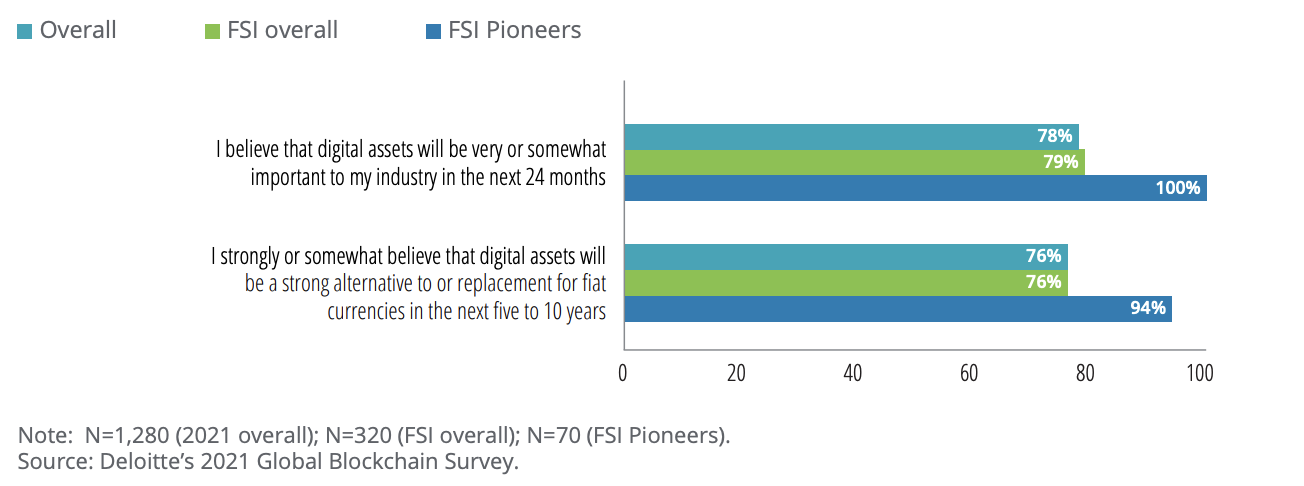
\includegraphics[width=\textwidth]{digital_assets_future.png}
  \caption{The future of digital assets (*) \cite{blockchainSurvey}}
  \label{fig:digital_assets_future}
\end{figure}

(*) FSI = Financial Services Industry. FSI Pioneers are respondents whose organizations have already deployed blockchain solutions into production and/or integrated digital assets into their core business activities. \\

\begin{figure}[H]
  \centering
  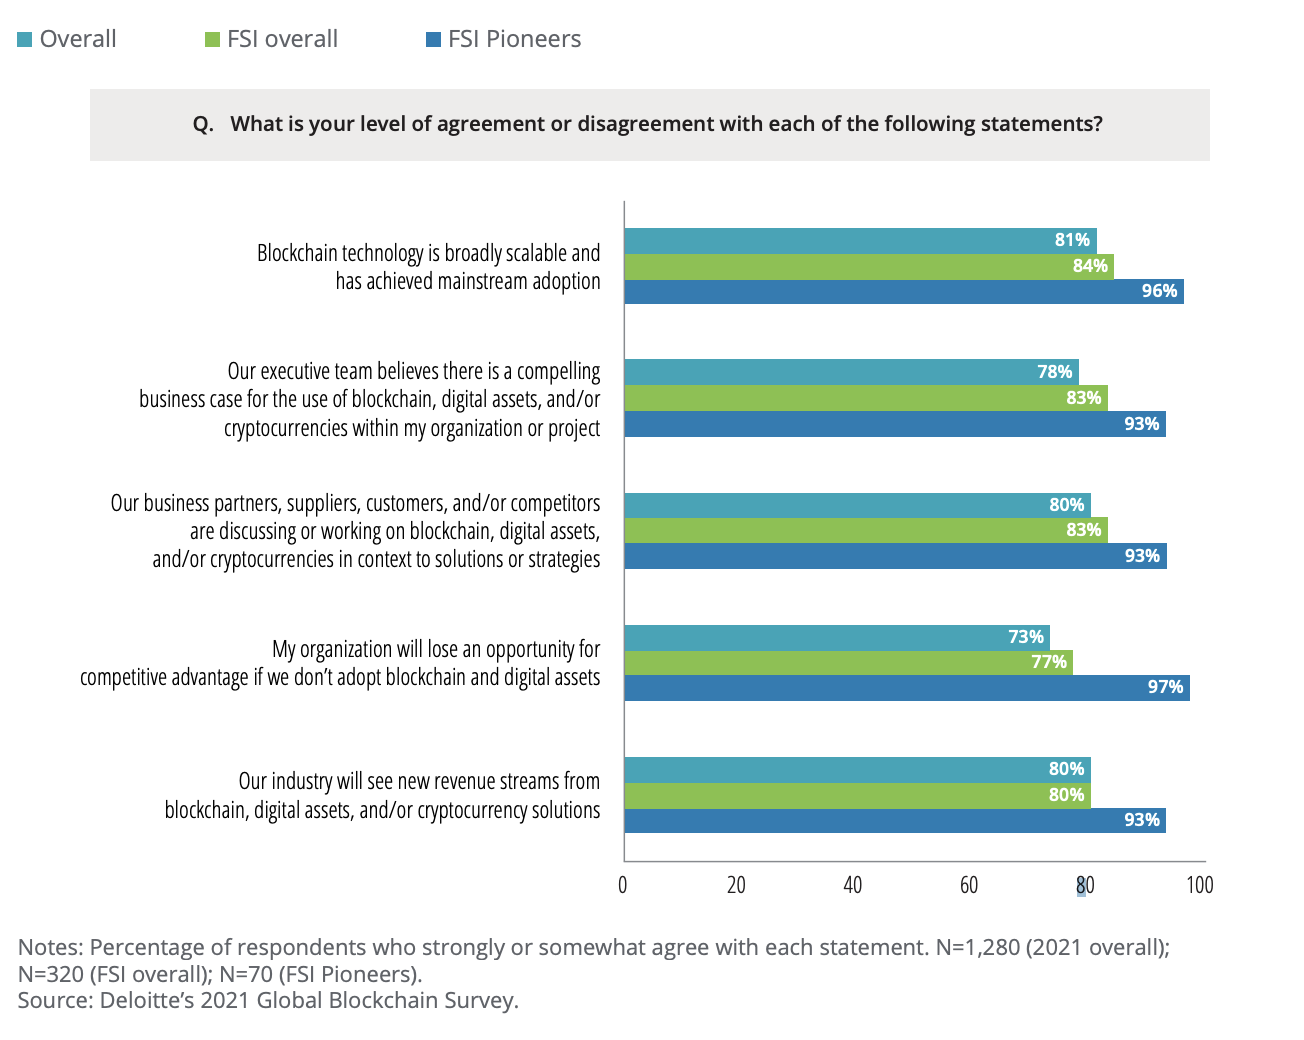
\includegraphics[width=\textwidth]{fsi_digital_assets.png}
  \caption{How do financial executives view blockchain and digital assets? \cite{blockchainSurvey}}
  \label{fig:fsi_digital_assets}
\end{figure}

\begin{figure}[H]
  \centering
  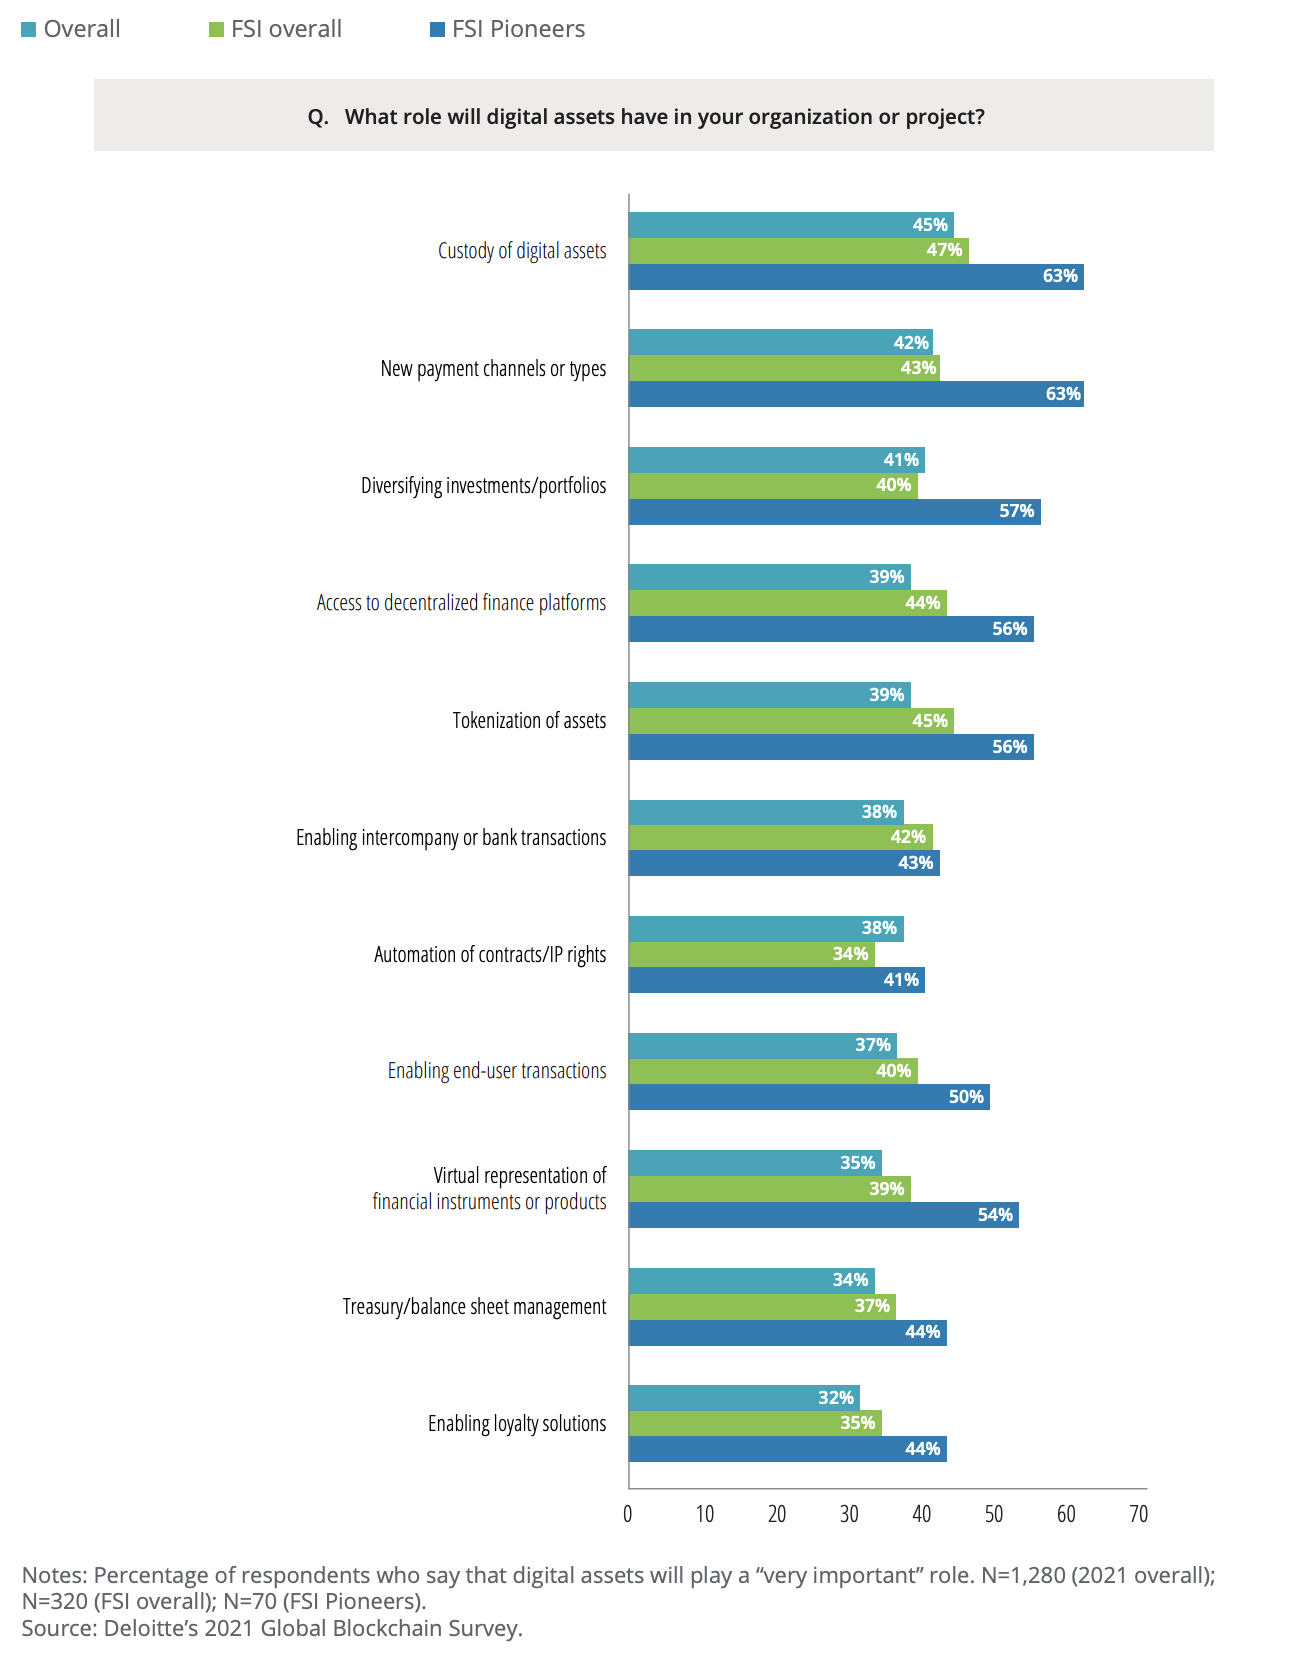
\includegraphics[width=\textwidth]{digital_assets_role.png}
  \caption{The role of digital assets in future \cite{blockchainSurvey}}
  \label{fig:digital_assets_role}
\end{figure}

What made it different from normal bank transfers or other financial services like Paypal is that there was no middle man for the first time. A middleman is a central authority like a bank or government that intervenes in a transaction between the sender and recipient. They have the power to surveil, censor, or revert transactions and they can share the sensitive data they collect with third parties. They also often dictate which financial services people have access to.\cite{ethereum} \\

There are many different types of digital assets.\cite{digAssets} Here is a list of many of the familiar ones:
\begin{multicols}{2}
  \begin{itemize}
    \item Photos
    \item Documents
    \item Videos
    \item Books
    \item Audio/Music
    \item Animations
    \item Illustrations
    \item Manuscripts
    \item Emails and email accounts
    \item Logos
    \item Metadata
    \item Content
    \item Social media accounts
    \item Gaming accounts
  \end{itemize}
\end{multicols}

Newer digital assets are based on blockchain or similar technologies:
\begin{multicols}{2}
  \begin{itemize}
    \item Non-Fungible Tokens
    \item Cryptocurrency
    \item Tokens
    \item Crypto Assets
    \item Tokenized Assets
    \item Security Tokens
    \item Central Bank Digital Currencies
  \end{itemize}
\end{multicols}

It is worth devoting a few paragraphs to the Non-Fungible Tokens (\glspl{NFT}): for the purposes of definition, a non-fungible token\cite{nft} can be seen as a unit of digital information (token) that is stored on a blockchain and is not inherently interchangeable with other digital assets (non-fungible). The term "fungible" derives from the economic and accounting literatures, and is defined as anything that is interchangeable with an identical or similar object. Traditional form of currency, whether equivalent sums of paper money or identical unit of precious metals, are fungible objects, and this is what helps them to serve as mediums of exchange, because they are understood to be of equal value. One can substitute a five-dollar bill with five one-dollar bills because both are fungible.

Assets that are commonly considered fungible are regulated commodities, common shares (stocks), financial options, and bills of money. By contrast, a non-fungible asset may be a person's car, for example, since someone borrowing a friend's car would not repay their debt to their friend by giving them another person's car. Collectible items such as baseball cards represent a traditional example of non-fungible assets, since each card would have unique attributes which enhance or diminish their value compared to other baseball cards. In the virtual realm, objects were originally thought to be difficult in terms of proving their uniqueness and distinguishability so that they could be considered "non-fungible".

\section{Smart contracts\label{sm}}
\emph{"A smart contract is a computerized transaction protocol that executes the terms of a contract. The general objectives of smart contract design are to satisfy common contractual conditions (such as payment terms, liens, confidentiality, and even enforcement), minimize exceptions both malicious and accidental, and minimize the need for trusted intermediaries. Related economic goals include lowering fraud loss, arbitration and enforcement costs, and other transaction costs."} Nick Szabo, 1994.\cite{smartContracts} \\

Smart contracts live on the Ethereum blockchain  (see \ref{eth}). They only execute when triggered by a transaction from a user (or another contract). These programs are called \ac{Dapp}.

Once a smart contract is published to Ethereum, it will be online and operational for as long as Ethereum exists. Not even the author can take it down. Since smart contracts are automated, they do not discriminate against any user and are always ready to use.\cite{ethereum}

\section{Ethereum\label{eth}}
Ethereum is a technology for building apps and organizations, holding assets, transacting and communicating without being controlled by a central authority. There is no need to hand over personal details to use it - the user remains in control of their own data and what is being shared. Ethereum has its own cryptocurrency, Ether, which is used to pay for certain activities on the Ethereum network.

Also it is \textbf{programmable} using \textbf{smart contracts}, so that means that people can build apps that use the blockchain to store data or control what apps can do. This results in a general purpose blockchain that can be programmed to do anything.\cite{ethereum}

\subsection{How did it begin?}
Although the Ethereum blockchain has a number of founders, Vitalik Buterin\cite{ethHistory} was the one who initially published a white paper explaining the concept of Ethereum in November 2013. Following Buterin's initial work, other brains jumped on board in various capacities to help bring the project to fruition.

It gained awareness in early 2014 when Buterin brought the concept of the blockchain project into the public eye at a Bitcoin conference in Miami Florida. The project raised capital via an initial coin offering (ICO) later the same year, selling millions of dollars worth of ETH coins in exchange for funds to use for the development of the project. Between July 22 and Sept. 2, 2014, the asset sale sold over \$18 million worth of ETH, paid for in Bitcoin.

Although ETH coins were purchasable in 2014, the Ethereum blockchain did not actually go live until July 30, 2015, meaning ETH buyers had to wait for the blockchain to launch before they could move or use their ETH. 

Called Frontier, the first iteration of the Ethereum blockchain simply got the chain off the ground and running, hosting smart contracts and proof-of-work mining. The initial launch gave folks the opportunity to set up their mining apparatuses and start building on the network.

\subsection{Proof-of-Work (PoW) vs. Proof-of-Stake (PoS)}
The Ethereum network began by using a consensus mechanism that involved \ac{PoW}\cite{PoW}. This allowed the nodes of the Ethereum network to agree on the state of all information recorded on the Ethereum blockchain and prevented certain kinds of economic attacks. However, Ethereum switched off proof-of-work in 2022 and started using proof-of-stake instead.

Proof-of-work is the underlying algorithm that sets the difficulty and rules for the work miners do on proof-of-work blockchains. Mining is the "work" itself. It's the act of adding valid blocks to the chain. This is important because the chain's length helps the network follow the correct fork of the blockchain. The more "work" done, the longer the chain, and the higher the block number, the more certain the network can be of the current state of things. \\

On Sept. 15, 2022 Ethereum switched to \ac{PoS}\cite{PoS}. In proof-of-work, miners prove they have capital at risk by expending energy. Ethereum uses proof-of-stake, where validators explicitly stake capital in the form of ETH into a smart contract on Ethereum. This staked ETH then acts as collateral that can be destroyed if the validator behaves dishonestly or lazily. The validator is then responsible for checking that new blocks propagated over the network are valid and occasionally creating and propagating new blocks themselves. \\

Proof-of-stake comes with a number of improvements to the now-deprecated proof-of-work system:

\begin{itemize}
  \item Better energy efficiency - there is no need to use lots of energy on proof-of-work computations
  \item Lower barriers to entry, reduced hardware requirements - there is no need for elite hardware to stand a chance of creating new blocks
  \item Reduced centralization risk - proof-of-stake should lead to more nodes securing the network
  \item Because of the low energy requirement less ETH issuance is required to incentivize participation
  \item Economic penalties for misbehaviour make 51\% style attacks exponentially more costly for an attacker compared to proof-of-work
  \item The community can resort to social recovery of an honest chain if a 51\% attack were to overcome the crypto-economic defenses.
\end{itemize}

\subsection{Statistics}

In the figure \ref{fig:dailyTxs} can be observed that the daily amount of transactions ranges between 1M and 1.25M since late 2020, with a peak of 1.7M daily transactions in May 2021.
\begin{figure}[H]
  \centering
  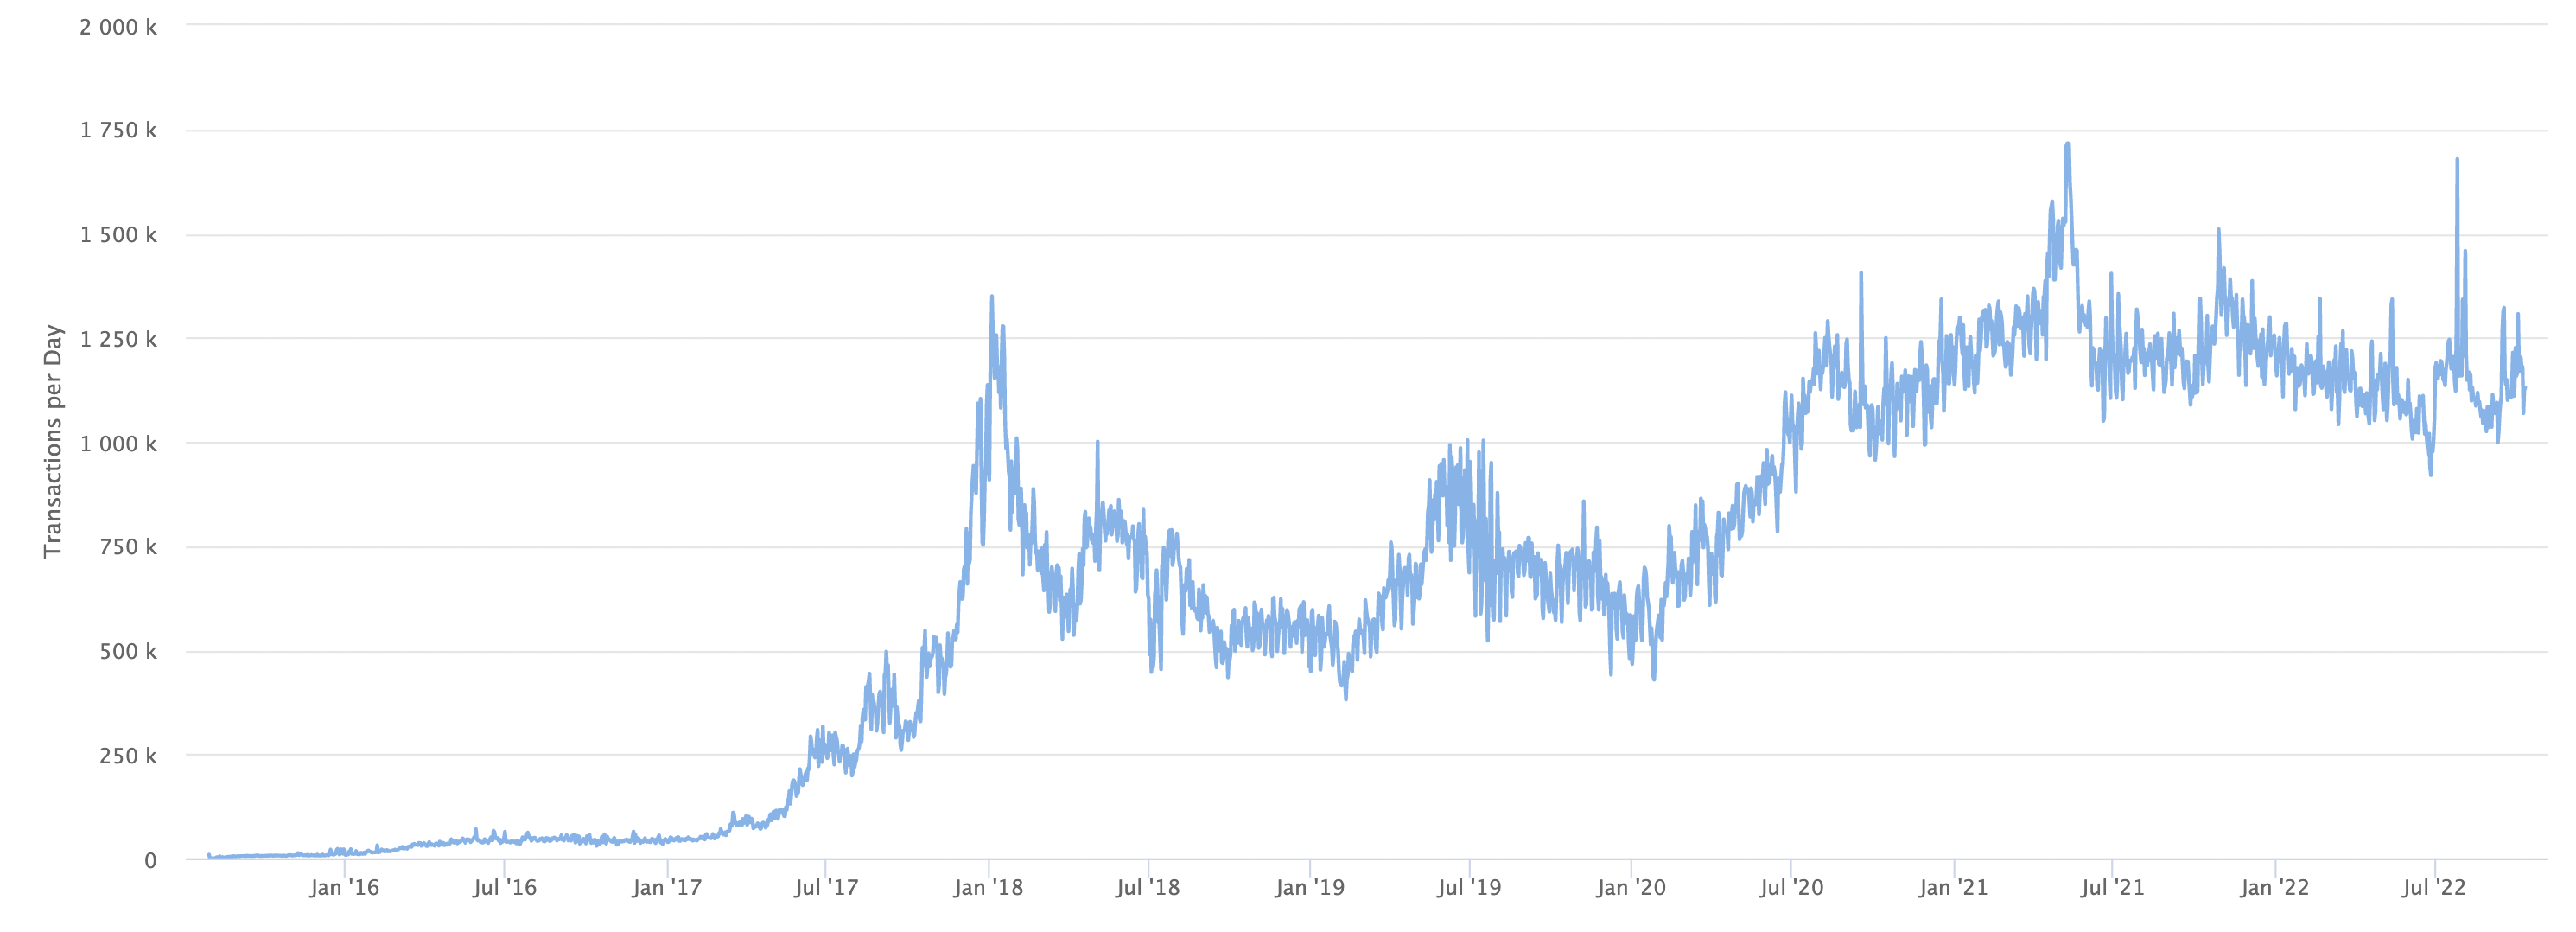
\includegraphics[width=\textwidth]{daily_txs.png}
  \caption{Daily Ethereum transactions \cite{etherscan}}
  \label{fig:dailyTxs}
\end{figure}

There are more than 200 million unique addresses in Ethereum as shown in the figure \ref{fig:uniqueAddr}.
\begin{figure}[H]
  \centering
  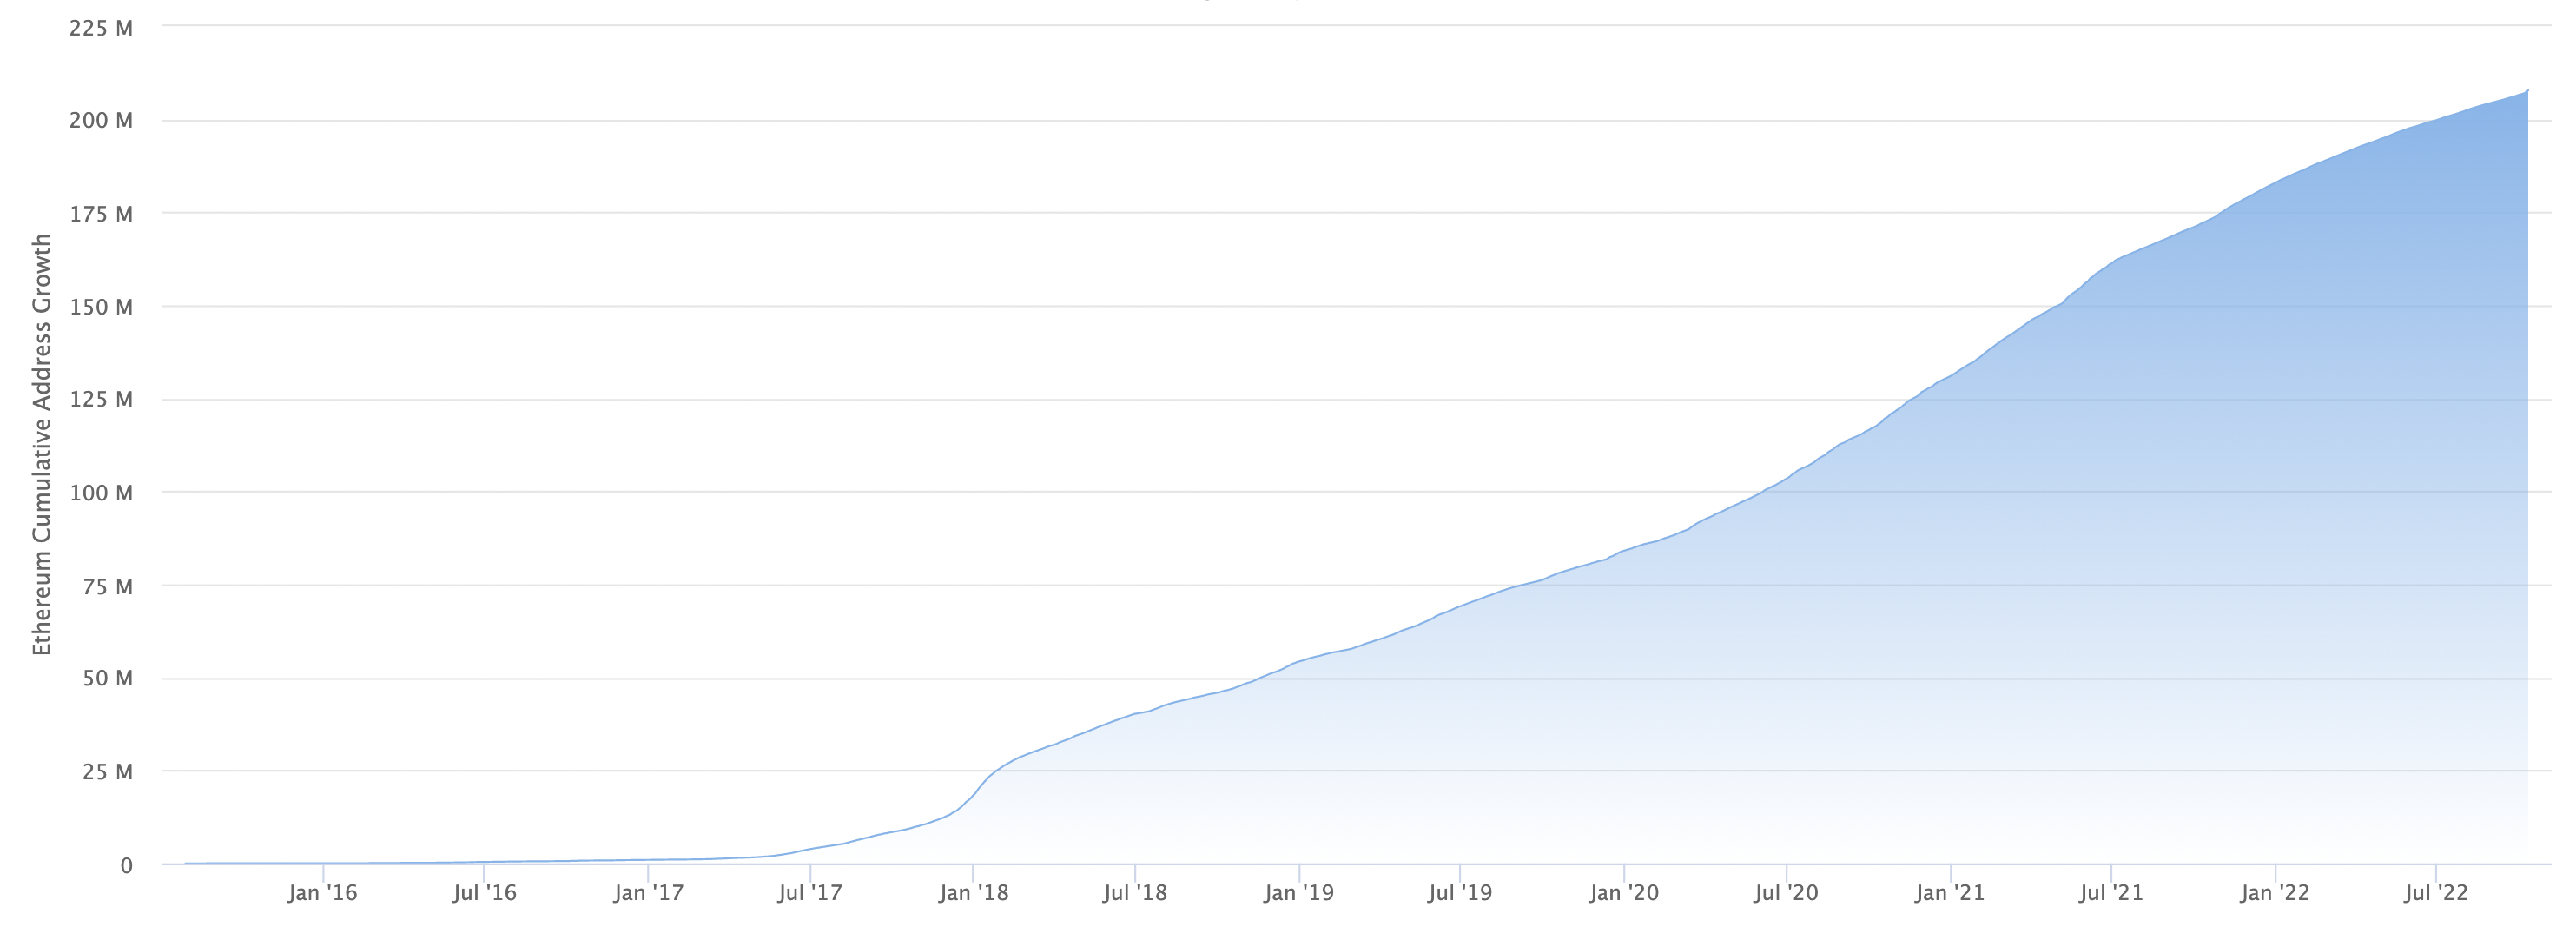
\includegraphics[width=\textwidth]{unique_addresses.png}
  \caption{Unique Ethereum addresses \cite{etherscan}}
  \label{fig:uniqueAddr}
\end{figure}

But only between 400,000 and 600,000 addresses are currently active, meaning between 0.2\% and 0.3\% of the unique addresses (see figure \ref{fig:activeAddr}).
\begin{figure}[H]
  \centering
  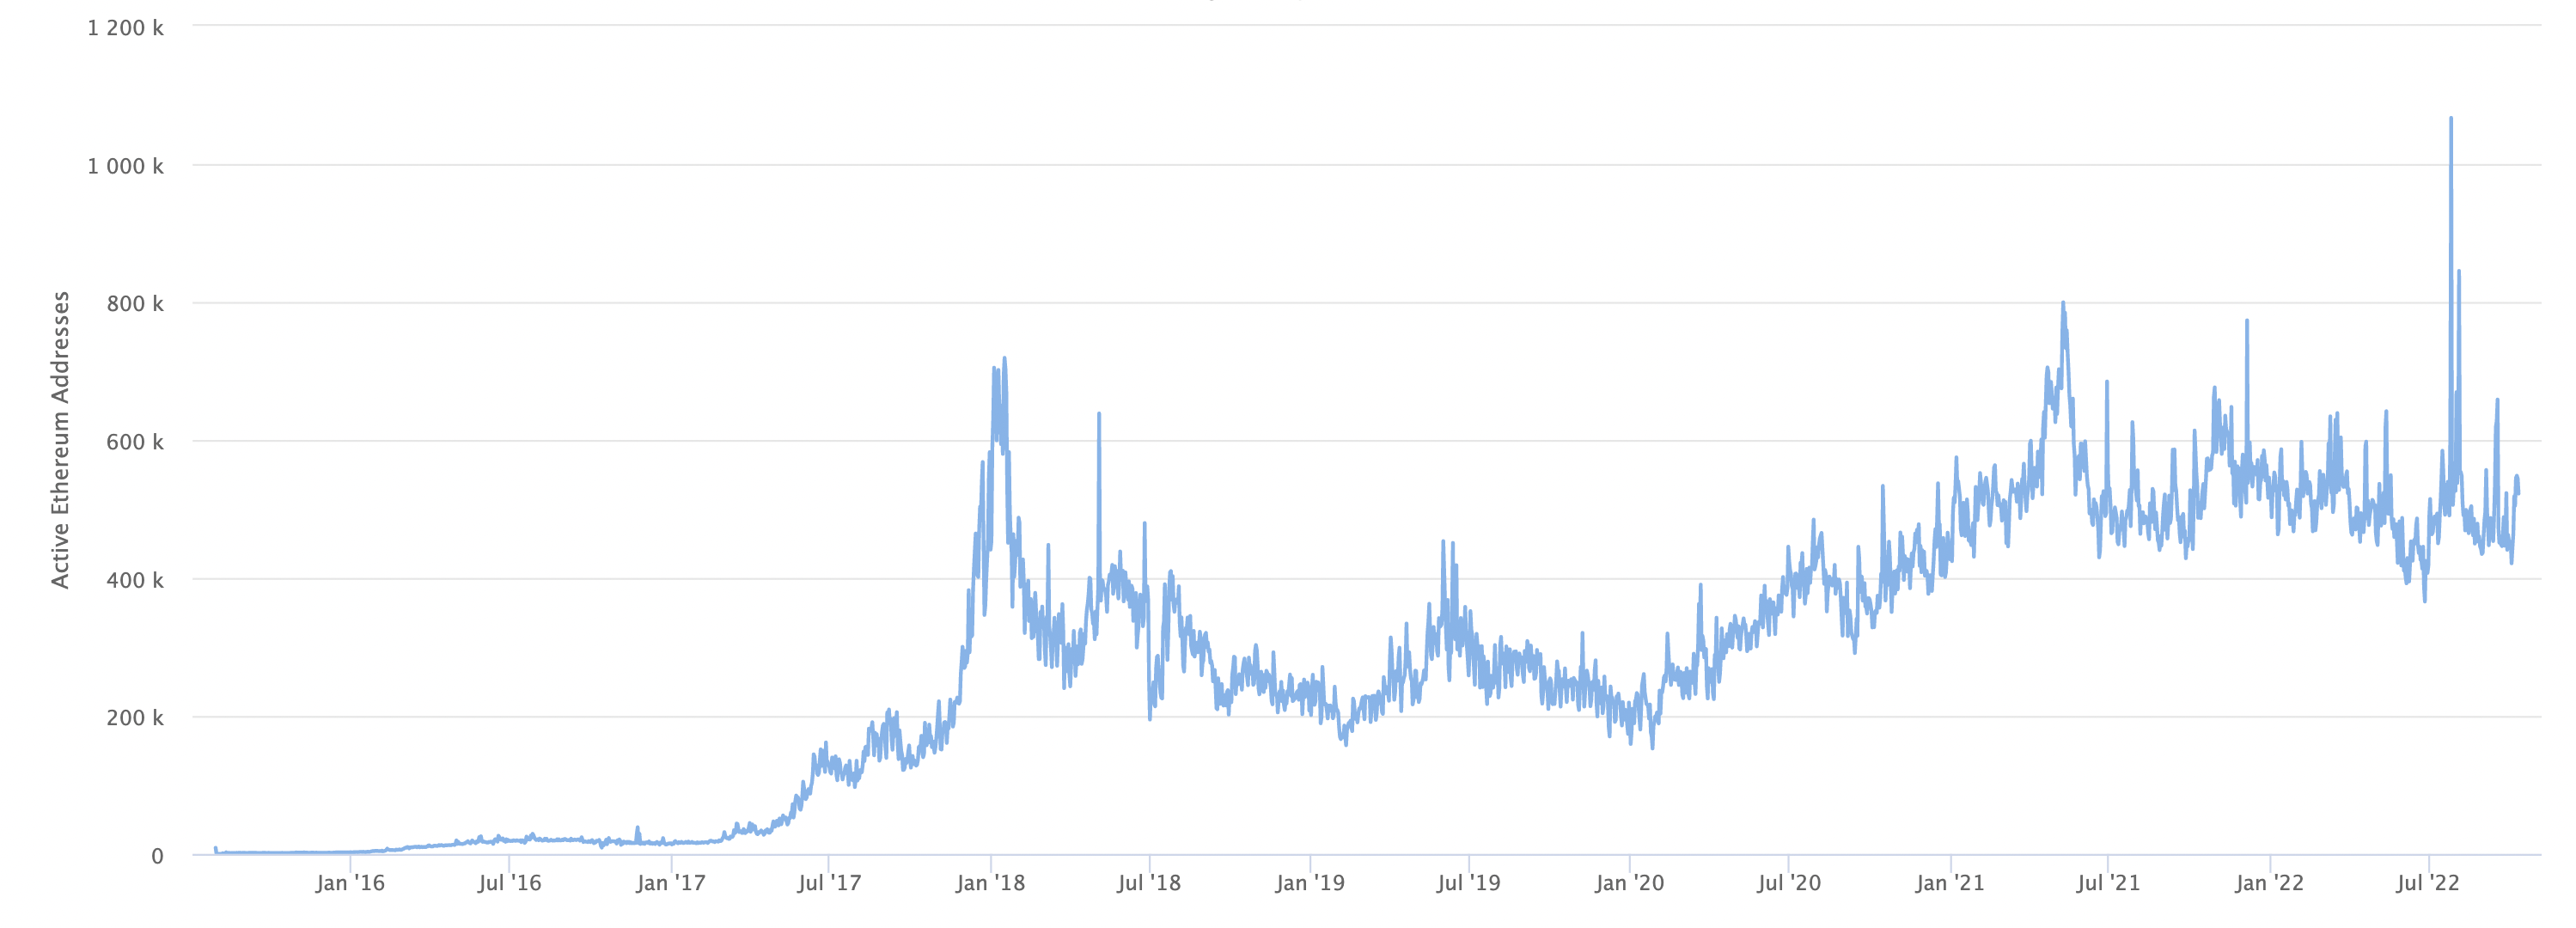
\includegraphics[width=\textwidth]{active_addresses.png}
  \caption{Active Ethereum addresses \cite{etherscan}}
  \label{fig:activeAddr}
\end{figure}

\section{Layer 2 solutions\label{layer2}}
\ac{L2}\cite{l2} is a collective term to describe a specific set of Ethereum scaling solutions. \textbf{A layer 2 is a separate blockchain that extends Ethereum and inherits the security guarantees of Ethereum.}

\subsection{What is a layer 1?}
Layer 1 is the base blockchain. Ethereum and Bitcoin are both layer 1 blockchains because they are the \textbf{underlying foundation that various layer 2 networks build on top of.} Examples of layer 2 projects include "rollups" on Ethereum and the Lightning Network on top of Bitcoin. All user transaction activity on these \ac{L2} projects can ultimately settle back to the layer 1 blockchain.

Ethereum also functions as a data availability layer for layer 2s. \ac{L2} projects will post their transaction data onto Ethereum, relying on it for data availability. This data can be used to get the state of the layer 2, or to dispute transactions on them. \\

Ethereum as the layer 1 includes:

\begin{itemize}
  \item A network of node operators to secure and validate the network
  \item A network of block producers
  \item The blockchain itself and the history of transaction data
  \item The consensus mechanism for the network
\end{itemize}

\subsection{Why is a layer 2 needed?}
Three desirable properties of a blockchain are that it is \textbf{decentralized, secure, and scalable}. The blockchain trilemma states that a simple blockchain architecture can only achieve two out of three. Want a secure and decentralized blockchain? scalability needs to be sacrificed.

Ethereum has reached the network's current capacity with 1+ million transactions per day and high demand for each of these transactions. The success of Ethereum and the demand to use it has caused gas prices to rise substantially. Therefore the need for scaling solutions has increased in demand as well. This is where layer 2 networks come in. \\

The benefits of layer 2s are:
\begin{itemize}
  \item \textbf{Lower fees:} By combining multiple off-chain transactions into a single layer 1 transaction, transaction fees are massively reduced, making Ethereum more accessible for all
  \item \textbf{Maintain security:} Layer 2 blockchains settle their transactions on Ethereum Mainnet, allowing users to benefit from the security of the Ethereum network
  \item \textbf{Expand use cases:} With higher transactions per second, lower fees, and new technology, projects will expand into new applications with improved user experience
\end{itemize}

As for the drawbacks of layer 2 solutions, it can be said that: \\

To begin with, L2 can degrade the underlying chain's liquidity.\cite{l2Drawbacks} Ethereum, for example, requires a liquid market to provide adequate support for all of its goods and tokens. However, once an additional layer is added, the blockchain's liquidity is likely to suffer.

Aside from that, users may encounter unnecessary onboarding issues. Once an extra layer is added, the L1 chain and its dApps will need to create new accounts. As a result, if funds are sent to multiple L2 protocols, the user may struggle to keep track of them all.

Finally, in certain cases, there may be security and privacy vulnerabilities.

\section{\NoCaseChange{\acl{DAO}} (DAO)}
A DAO is a collectively-owned, blockchain-governed organization working towards a shared mission.

DAOs allow people to work with like-minded individuals around the globe without trusting a benevolent leader to manage the funds or operations. There is no CEO who can spend funds on a whim or CFO who can manipulate the books. Instead, blockchain-based rules baked into the code define how the organization works and how funds are spent.

They have built-in treasuries that no one has the authority to access without the approval of the group. Decisions are governed by proposals and voting to ensure everyone in the organization has a voice, and everything happens transparently on-chain.\cite{DAO} \\

Table \ref{table:DAOComparison} compares a DAO with a traditional organization:
\begin{center}
  \begin{table}[H]
    \begin{tabular}{ | m{20em} | m{20em} | }
      \hline
      \textbf{DAO} & \textbf{Traditional organization} \\ 
      \hline
      Usually flat, and fully democratized. & Usually hierarchical. \\
      \hline  
      Voting required by members for any changes to be implemented. & Depending on structure, changes can be demanded from a sole party, or voting may be offered. \\
      \hline
      Votes tallied, and outcome implemented automatically without trusted intermediary. & If voting allowed, votes are tallied internally, and outcome of voting must be handled manually. \\
      \hline
      Services offered are handled automatically in a decentralized manner (for example distribution of philanthropic funds). & Requires human handling, or centrally controlled automation, prone to manipulation. \\
      \hline
      All activity is transparent and fully public. & Activity is typically private, and limited to the public. \\
      \hline
    \end{tabular}
    \caption{Comparison between a DAO and a traditional organization \cite{DAO}}
    \label{table:DAOComparison}
  \end{table}
\end{center}

\section{Metaverse\label{dcl}}
\emph{"The Metaverse is the post-reality universe, a perpetual and persistent multiuser environment merging physical reality with digital virtuality. It is based on the convergence of technologies that enable multisensory interactions with virtual environments, digital objects and people such as \ac{VR} and \ac{AR}. Hence, the Metaverse is an interconnected web of social, networked immersive environments in persistent multiuser platforms. It enables seamless embodied user communication in real-time and dynamic interactions with digital artifacts. Its first iteration was a web of virtual worlds where avatars were able to teleport among them. The contemporary iteration of the Metaverse features social, immersive VR platforms compatible with massive multiplayer online video games, open game worlds and AR collaborative spaces."} Stylianos Mystakidis, 2022. \cite{metaverse} \\

\begin{figure}[H]
  \centering
  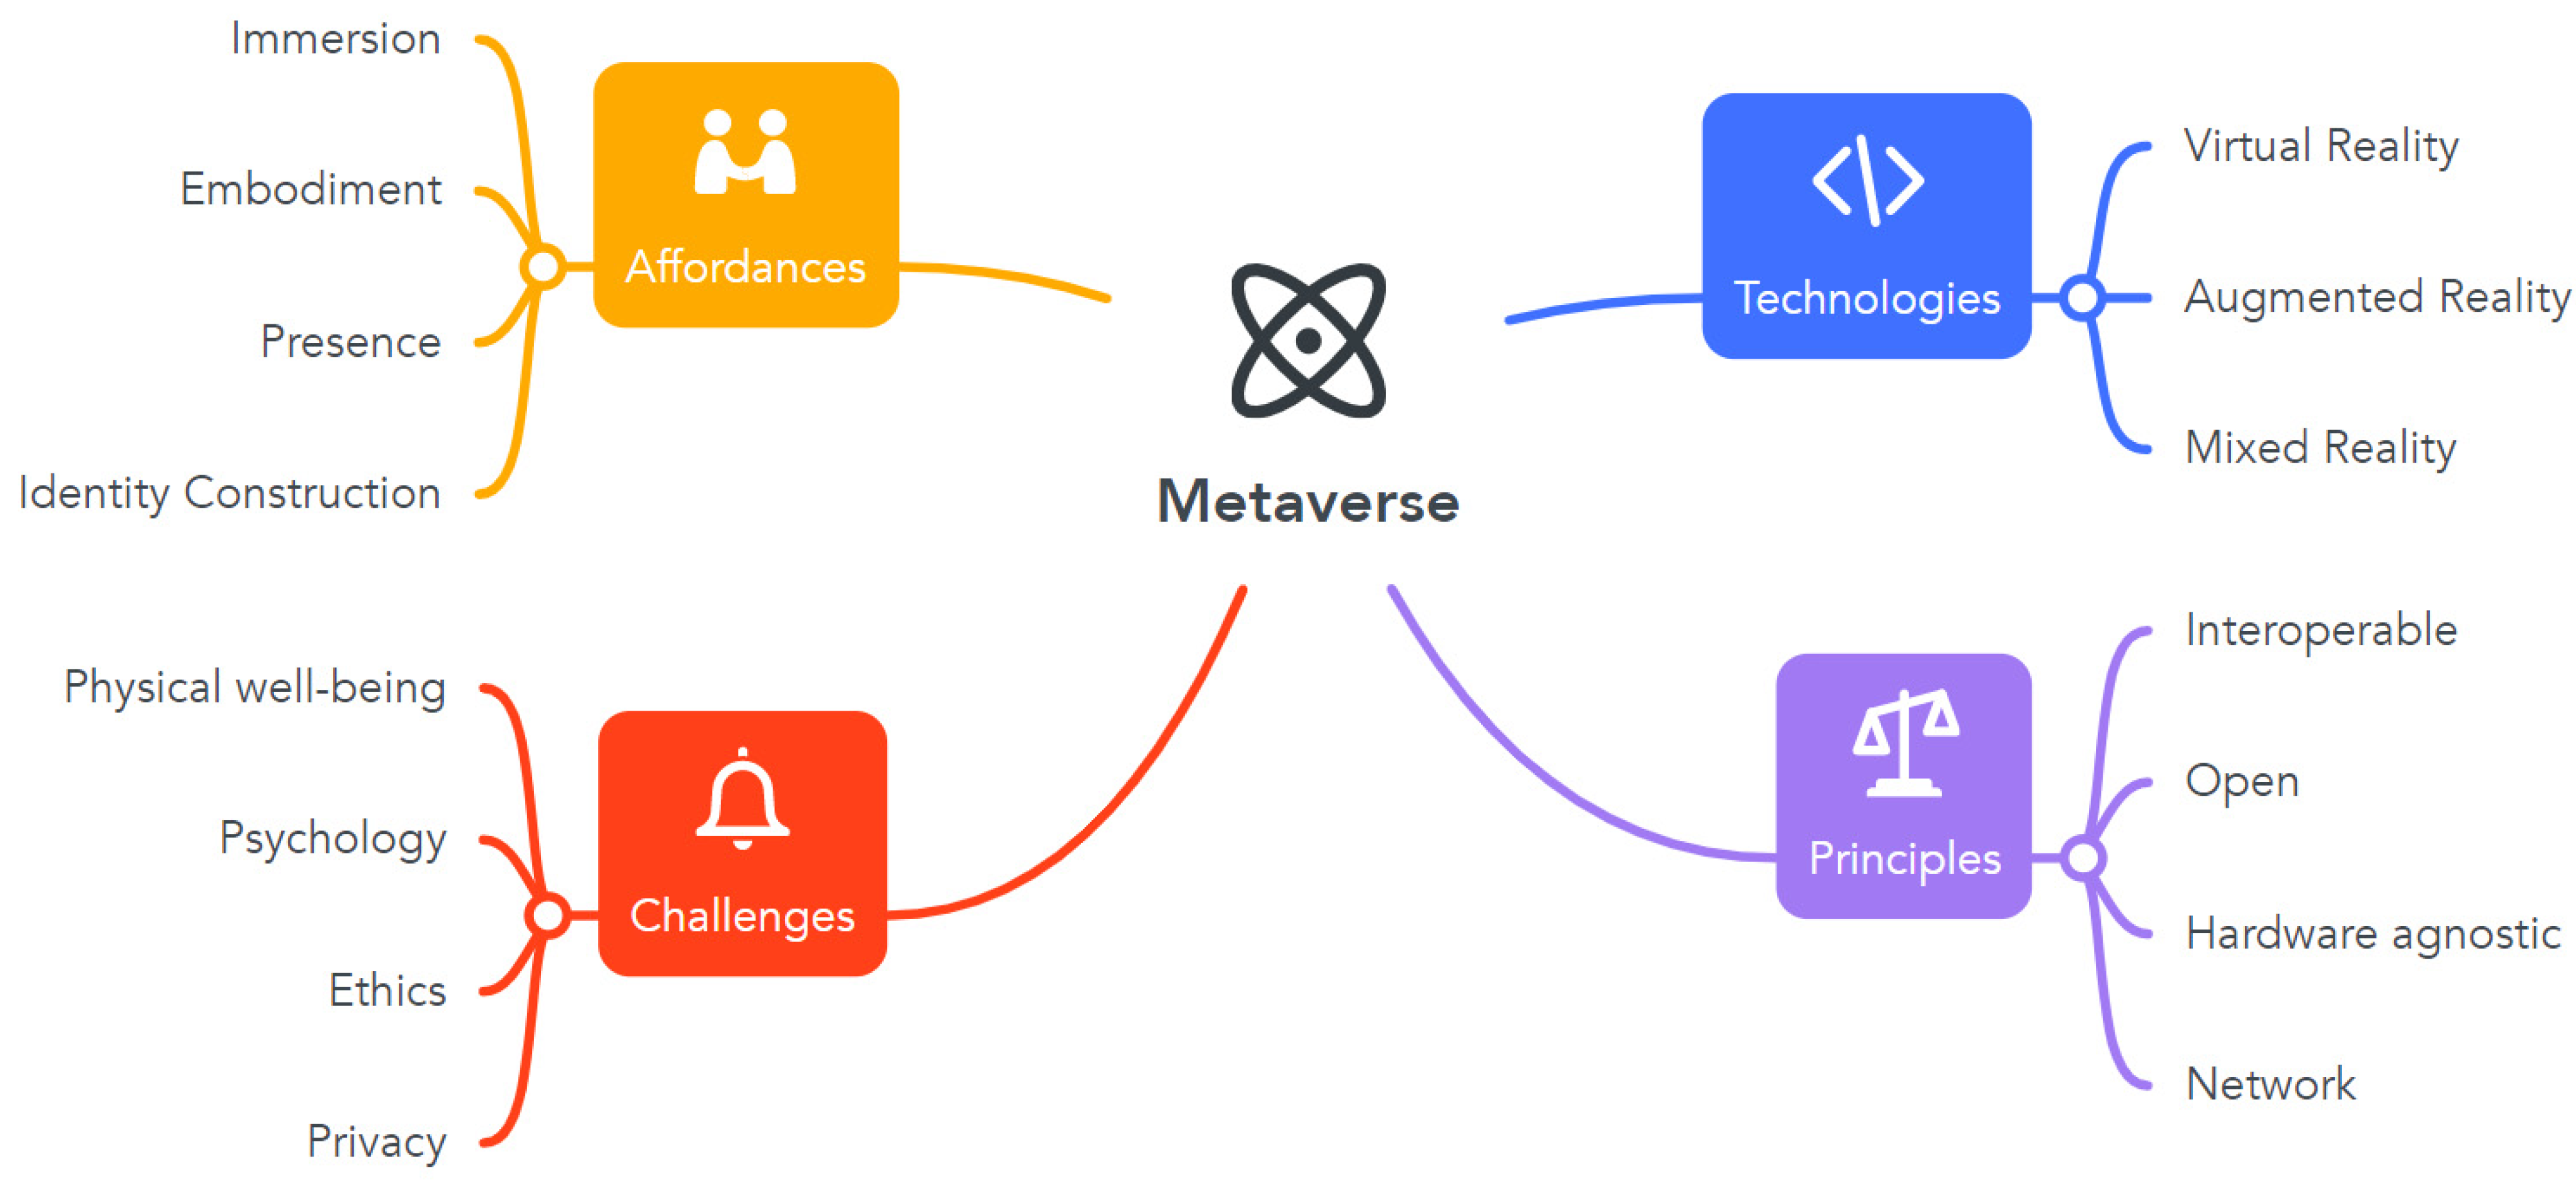
\includegraphics[width=\textwidth]{metaverse.png}
  \caption{Description of the metaverse \cite{metaverse}}
  \label{fig:metaverse}
\end{figure}

Decentraland\cite{DCL} is a decentralized virtual reality platform, better known as a metaverse, powered by the Ethereum blockchain. It is an open source project, maintained by the Decentraland Foundation and driven by its community. 

Within the Decentraland platform, users can create, experience, and monetize their content and applications. The finite, traversable, 3D virtual space within Decentraland is called \textbf{\gls{LAND}}, a non-fungible digital asset or more commonly known as a \ac{NFT}, maintained in an Ethereum smart contract. Land is divided into parcels that are identified by cartesian coordinates (x,y). These parcels are permanently owned by members of the community and are purchased using \textbf{\gls{MANA}}, Decentraland's cryptocurrency token. This gives users full control over the environments and applications that they create, which can range from anything like static 3D scenes to more interactive applications or games.

\begin{figure}[H]
  \centering
  
\includegraphics[width=\textwidth]{dcl.png}
  \caption{Screenshot of Decentraland}
  \label{fig:dcl}
\end{figure}

\begin{figure}[H]
  \centering
  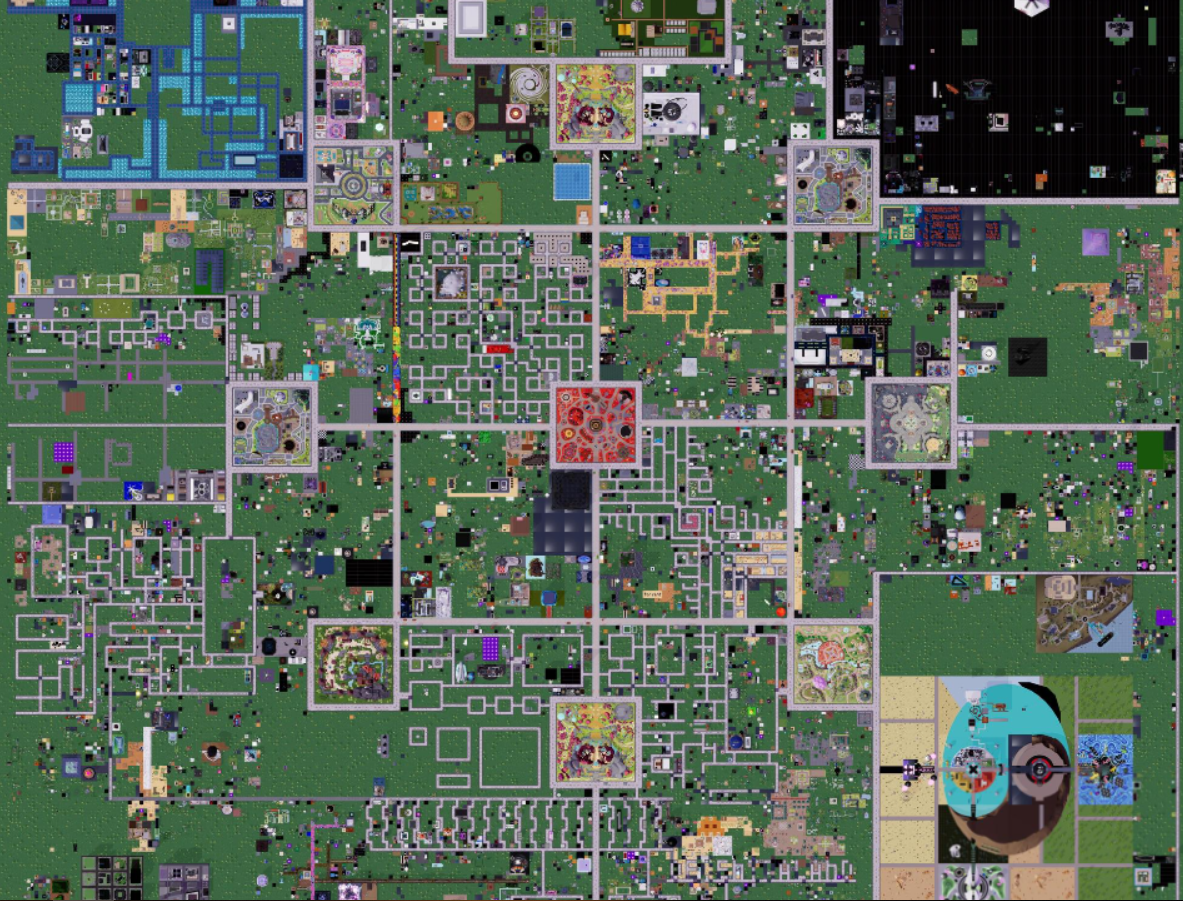
\includegraphics[width=.8\textwidth]{dcl_map.png}
  \caption{Top view of Decentraland's map \cite{genesisCity}}
  \label{fig:dcl_map}
\end{figure}

The Decentraland DAO\cite{DCLDAO} is the decision-making tool for digital assets holders in Decentraland's virtual world. Through votes in the DAO, the community can issue grants and make changes to the lists of banned names, POIs, and catalyst nodes. The DAO also controls the \gls{LAND} and \gls{ESTATE} smart contracts.

These proposals, the votes submitted, and final results are all stored in IPFS via Snapshot, a gas-less voting client. Approved proposals with binding actions are enacted on the Ethereum blockchain by a committee by means of a multi-sig wallet. This committee is overseen by the Security Advisory Board (SAB), another multisig with trusted key holders. This Committee was voted into place by the community in the previous release of the DAO.

\chapter{Methodology\label{method}}
\section{Problem}
Decentraland is open source and community driven. As a consequence, many stakeholders are involved in decision-making. It is essential to have as much information as possible about the status of the project available, in order to make informed decisions.

So far, there was no tool or solution that could publicly provide information to everyone about the state of the DAO treasury and the different assets of the community. Of course, the information was and still is available since the blockchain is public, but not everyone has the time or knowledge to collect and analyze such data.

Therefore, in summary, there was a need to develop a tool that would provide information publicly on the state of the DAO's treasury and the different assets of the community to enable informed decision making. \\

To begin designing the solution, three main sources were considered: \\

1. First, the Decentraland community. It is necessary to understand the current needs to be able to propose a solution to the problem, that is why it was taken as main input the requests of the users through conversations and interviews. \\

2. The next was the team that maintains the DAO platform, known as the DAO Squad. From them were obtained the technical requirements needed to carry out the design of the tool and the implementation path.\\

3. Lastly, the data team from the Decentraland Foundation. Once all the information was obtained, it is necessary to make sense of it through charts and analytics, which is why the support of this team was provided to represent all the valuable information in the best possible way.\\

\section{Research questions\label{research}}
The research questions that will be answered at the end of this work are: \\

\textbf{Q1. How easy is it for an average user to access public information on the blockchain?}

It is clear that most users do not have much technical knowledge and, for blockchain technology to be increasingly adopted, interacting with it must be simple enough for anyone to do so. \\

\textbf{Q2. What kind of analysis and conclusions can be drawn with the data obtained from the blockchain?}

Data by itself is just that: Data. Meaning must be given to that information so that conclusions can be drawn and informed decisions can be made.

\section{Methods\label{methods}}
After reviewing the community's requests, it was determined that the goal of this project must be about collecting and processing Decentraland's public data and making it available to stakeholders in a consumable format. The scope includes:

\begin{itemize}
  \item \textbf{Accounting:} Tracking different streams such as
  \begin{itemize}
    \item Income
    \item Expenses
    \item Revenue
    \item Balance
  \end{itemize}
  \item \textbf{Market:} Sizing transacted value in the world and liquidity
  \begin{itemize}
    \item Tracking sales data
    \item DAO and Creators revenue
    \item Estimation of economy size
    \item Defining health indicators
  \end{itemize}
  \item \textbf{Operations:} Defining business unit performance metrics
  \begin{itemize}
    \item Teams Performance
    \item Execution times, operative expenses, etc.
    \item Does any team need to shrink or expand?
  \end{itemize}
\end{itemize}

\subsection{Requirements}
For the solution of this problem, the following requirements were mandatory:
\begin{enumerate}
  \item It must be possible to visualize the general state of the DAO's treasury and the different assets of the community.
  \item It must be possible to visualize metrics to be able to make decisions.
  \item Data collection must be from public sources.
  \item The data collection scripts must be open source.
  \item Both the information collected and the metrics performed must be accessible to anyone.
\end{enumerate}

\subsection{Data collection sources}
\subsubsection{Decentraland's Catalyst Nodes}
A Catalyst\cite{catalyst} is a Server that bundles different Services required by the Decentraland World. Some of the main responsibilities of the server are the management of the decentralized storage for most of the content needed by the client and the orchestration of communications between peers. Each Catalyst node exposes a set of services that work as the backbone for the platform and also exposes a public API.


\subsubsection{Infura}
Infura\cite{infura} is a blockchain development suite that provides application programming interfaces (APIs) and developer tools. It provides fast and reliable access to the Ethereum network to enable developers to build software and Web3 applications that scale to meet user demand.
As an Infrastructure-as-a-Service (IaaS) and Web3 backend infrastructure provider, it offers documentation and resources to help developers build decentralized applications (dApps) quickly. This is achieved by reducing the time spent building infrastructure from scratch. Infura offers enterprise-ready infrastructure using a distributed cloud-hosted network of nodes. This removes much of the friction associated with the development and ownership of proprietary computing and storage facilities. 

The Infura Ethereum API provides developers with easy-to-access Ethereum-based infrastructure to build decentralized applications. Using it, builders can connect applications in just a few seconds using a single line of code. This makes it simple to take advantage of fast, highly available Ethereum infrastructure. 

\begin{figure}[H]
  \centering
  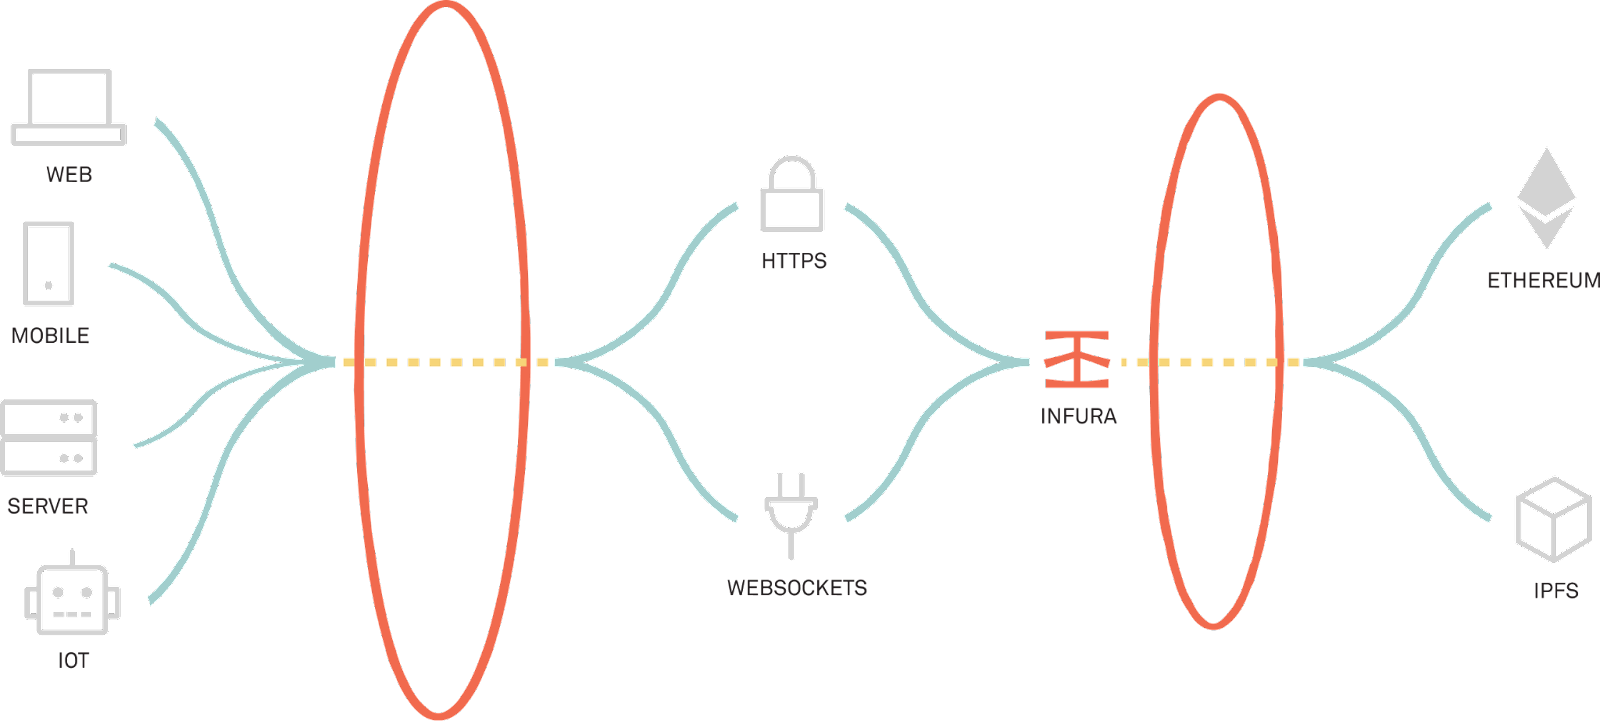
\includegraphics[width=\textwidth]{infura.png}
  \caption{Diagram of information flow through Infura \cite{infura}}
  \label{fig:infura}
\end{figure}

\subsubsection{The Graph}
The Graph\cite{thegraph} is a decentralized protocol for indexing and querying data from blockchains, starting with Ethereum. It makes it possible to query data that is difficult to query directly.

To get this data, every single transfer event issued would have to be processed, read the IPFS\footnote{\url{https://docs.ipfs.tech/concepts/what-is-ipfs/}} metadata using the token ID and IPFS hash, and then aggregated. Even for such relatively simple queries, a \ac{Dapp} running in a browser would take hours or even days to get an answer.

The Graph solves this with a decentralized protocol that indexes and enables the performant and efficient querying of blockchain data. These APIs (indexed "subgraphs") can then be queried with a standard GraphQL API. Today, there is a hosted service as well as a decentralized protocol with the same capabilities. Both are backed by the open source implementation of Graph Node.

\subsubsection{Snapshot}
Snapshot\cite{snapshot} is a decentralized voting system. It provides flexibility on how voting power is calculated for a vote. It supports various voting types to cater to the needs of organizations. Creating proposals and voting on Snapshot is user-friendly and does not cost gas as the process is performed off-chain.
In short, Snapshot is an off-chain gasless multi-governance client with easy to verify and hard to contest results. \\

Its key features are:
\begin{itemize}
  \item Free (gasless) to create proposals and vote on them
  \item Votes are signed messages easily verifiable online
  \item Multiple voting systems - Single choice, Approval voting, Quadratic voting, and more
  \item Flexible voting strategies to calculate voting results - vote with ERC20s, NFTs, other contracts, and more
  \item Fully open-source with MIT license
\end{itemize}

\subsubsection{Covalent}
Covalent\cite{covalent} is a multi-chain unified application programming interface that brings visibility to billions of data points for multiple blockchains. As an indexing querying solution for blockchains, the platform offers a diverse range of actionable insights that enable developers to optimize the allocation of resources, bringing greater utility to decentralized applications using a single, unified API.

Covalent collates millions of data points from different organizations. Rather than searching for data from multiple locations on multiple blockchains, the network provides a one-stop-shop for high-quality multi-chain data.

This is made possible by aggregating various data feeds from nodes on different blockchains. The Covalent API then facilitates the distribution of customized data feeds to suit the individual needs of users. This data can be broad or specific, depending on the application. For example, the API can provide both the historical and current performance of digital assets. This could be for a small handful of assets or to analyze the entire crypto market. Plus, when data is requested, it is returned quickly in a uniform, consistent manner. Regardless of how many blockchains are queried, all relevant data is presented in a single API.

\chapter{Solution\label{solution}}
To begin the implementation of such a tool that meets the requirements outlined in section \ref{methods}, it was decided to first establish a public repository\footnote{\url{https://github.com/Decentraland-DAO/transparency}} within the Decentraland DAO organization where the scripts code and version histories would be stored. In this way, the tool is auditable by anyone who is willing to do so.

Since data must be collected every day and different sources must be consumed, Node.js was chosen for the backend of the project as it is easily configurable to run periodically in a GitHub Action\footnote{\url{https://github.com/actions/setup-node}}. As for the programming language chosen, Typescript was used due to the versatility it offers and, naturally, for the typing, since it is very useful when working with data. The collected information is available in two widely used formats: \textbf{CSV} \& \textbf{JSON}. The first one is very useful for data analysis and the second one can be consumed by other applications.

Finally, Google Data Studio\footnote{\url{https://datastudio.google.com/u/0/reporting/fca13118-c18d-4e68-9582-ad46d2dd5ce9/page/p_nlc90z86rc}} is used to visualize the metrics, which uses as input the information from the CSVs collected with the scripts (previously uploaded to a Google spreadsheet). This allows the community to have a simple way to visualize metrics that can be easily shared with other people.

\section{From data to metrics}
\begin{figure}[H]
  \centering
  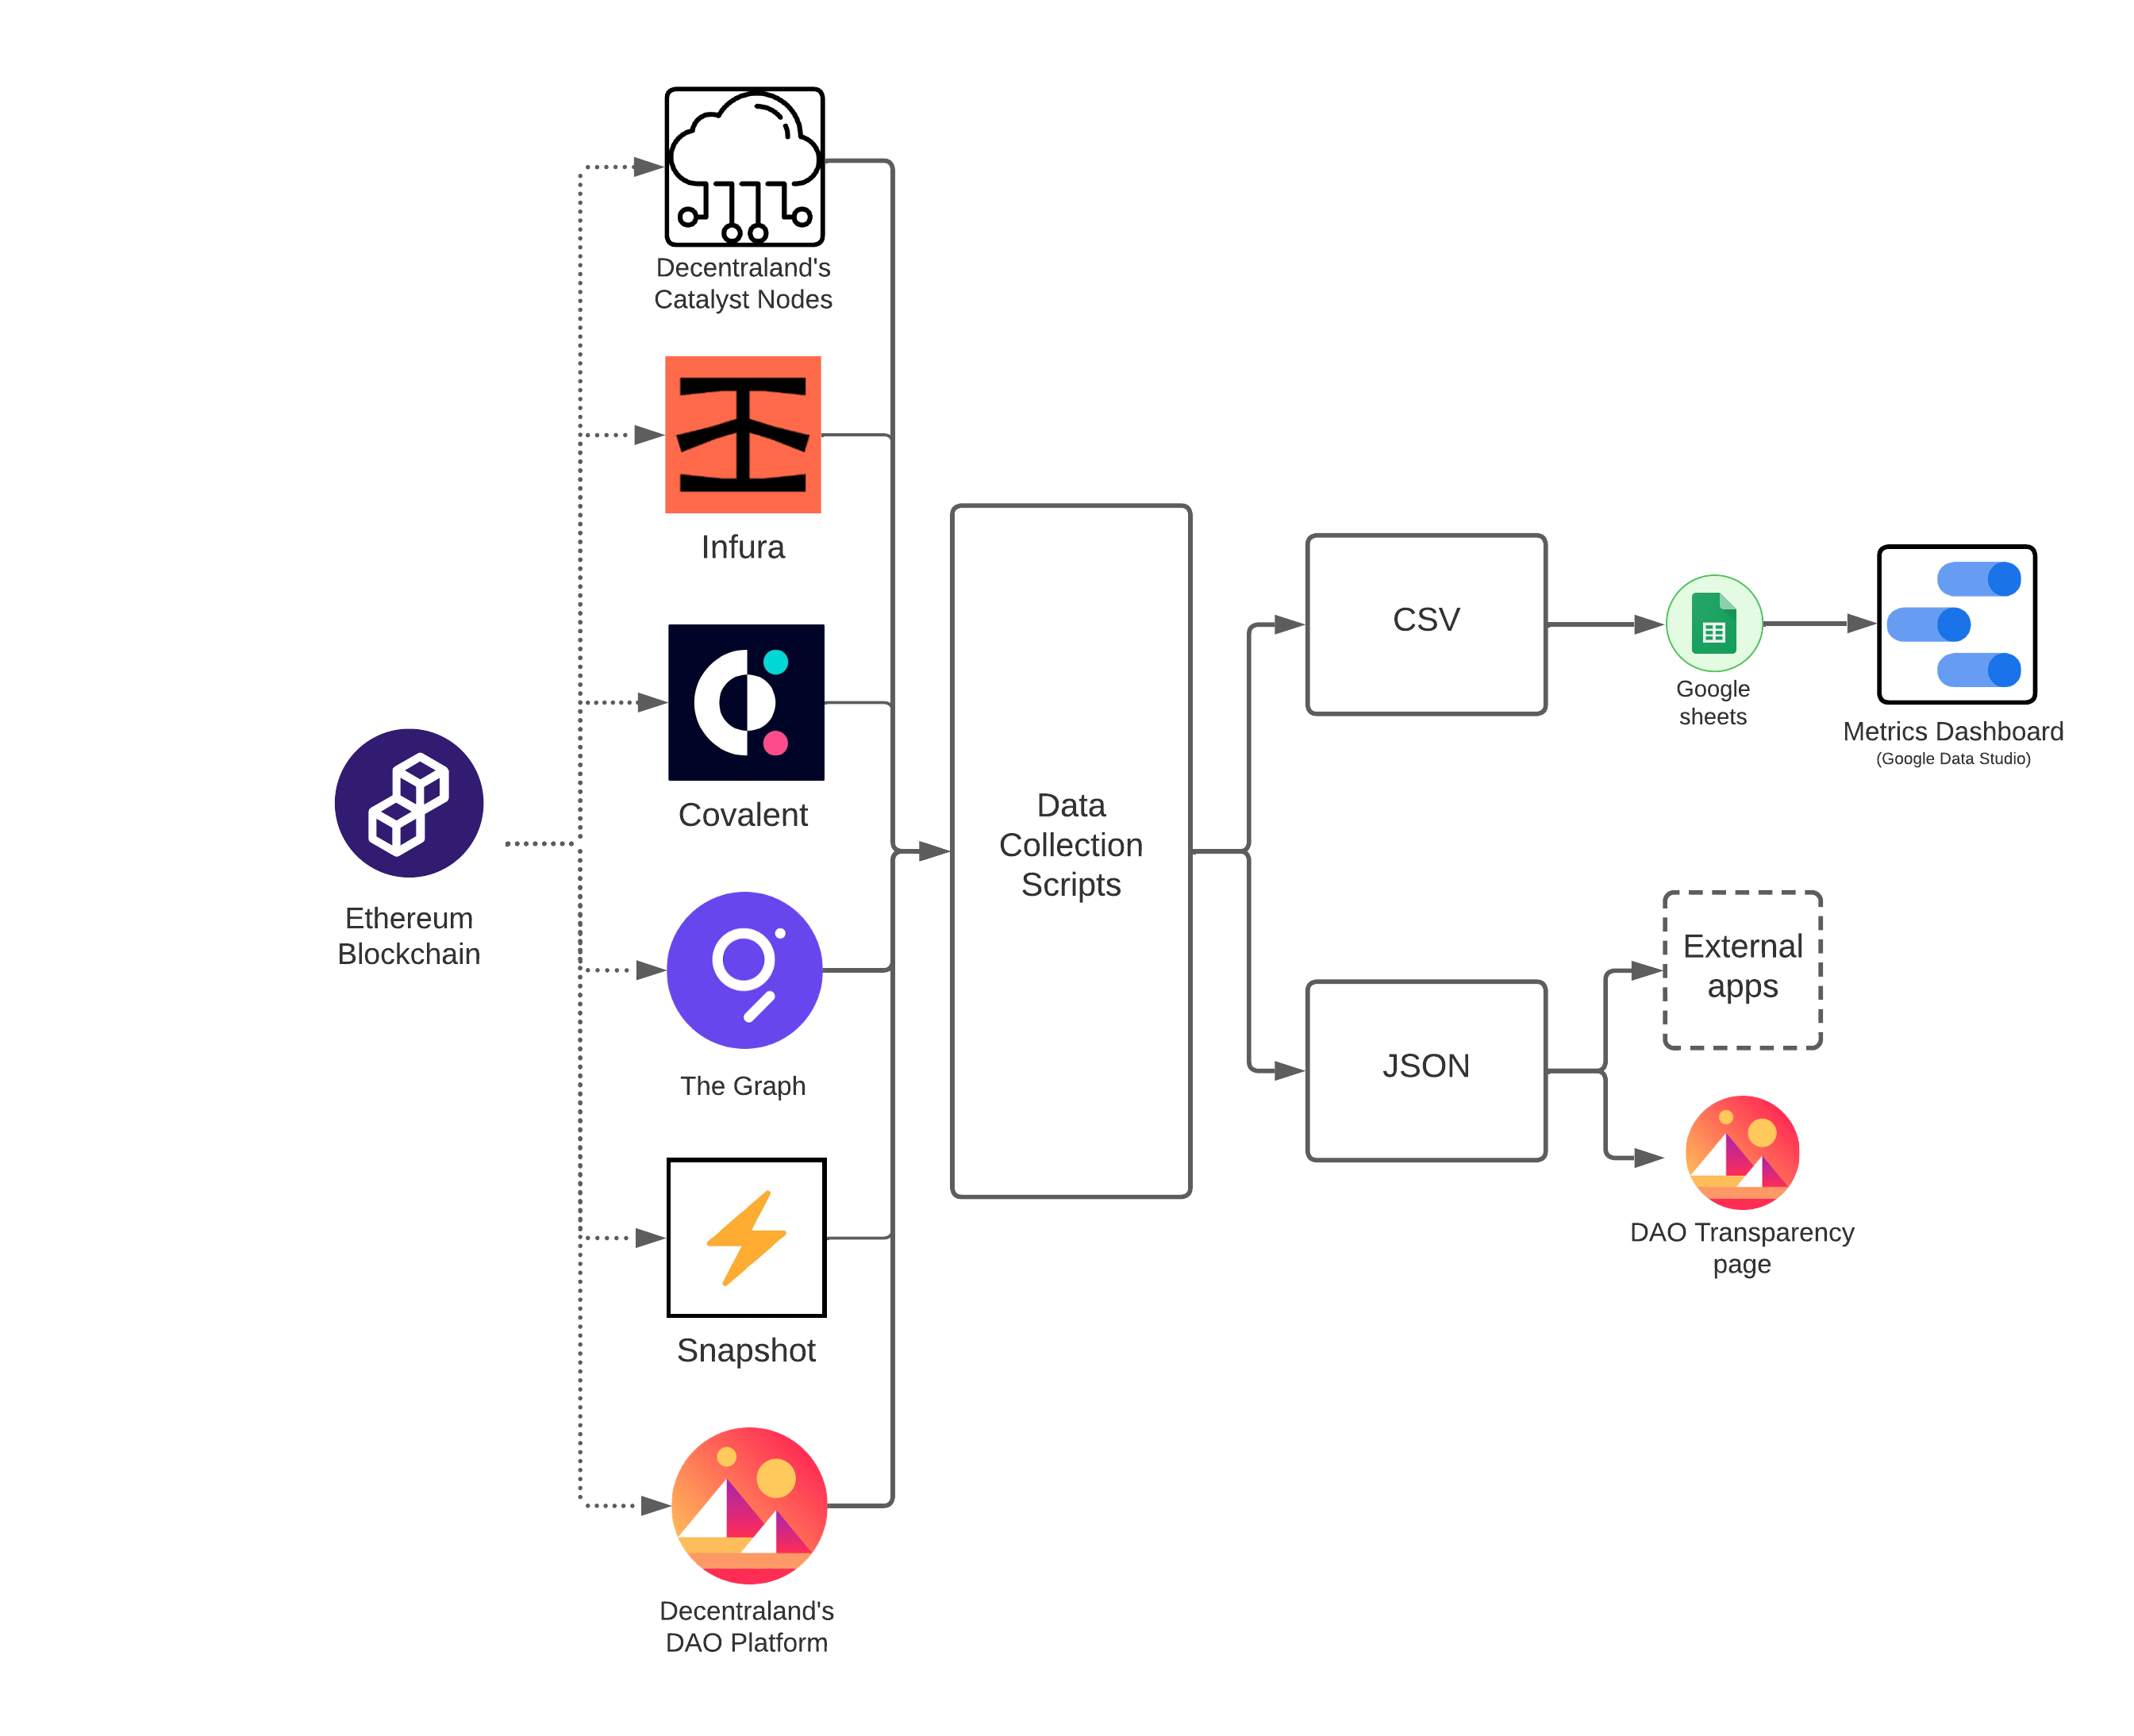
\includegraphics[width=\textwidth]{diagrama.png}
  \caption{Data collection diagram}
  \label{fig:diagram}
\end{figure}

It all starts with the services that index blockchain information such as Infura, Covalent or The Graph and those that add custom information such as Snapshot, Decentraland's catalyst nodes or even the platform's governance Dapp.

In order to collect the data, certain scripts were developed and will be explained below. To check the code of these scripts and their historical changes, it can be done from the GitHub repository\footnote{\url{https://github.com/Decentraland-DAO/transparency}} and the link can be found at the bottom of this page.

\subsection{Data collection scripts}
\subsubsection{Balances}
The first script is very simple and it's responsible for collecting the balances of the DAO's treasury. This is done by making a Covalent API call using the DAO's wallet addresses. The result is a JSON and CSV file with the amount of the different tokens with the values also expressed in US Dollars. \\

The fields included are:
\begin{itemize}
  \item \textbf{Timestamp}: [ISODate] The date on which the balance query was made
  \item \textbf{Wallet}: [String] The name of the wallet
  \item \textbf{Balance}: [Number] The amount of tokens in the wallet
  \item \textbf{Symbol}: [String] The symbol of the token
  \item \textbf{USD Balance}: [Number] The value of tokens expressed in US Dollars
  \item \textbf{USD Rate}: [Number] The current exchange rate of the token
  \item \textbf{Network}: [String] The network on which such wallet is located (either Ethereum or Polygon)
  \item \textbf{Address}: [String] The wallet's address
  \item \textbf{Token}: [String] The smart contract's address of the token
\end{itemize}

\subsubsection{Collections}
The second script is also very simple and it's responsible for collecting the data about all wearable collections that are currently available in Decentraland. This is done by making a GraphQL\footnote{\url{https://graphql.org/}} query to the corresponding subgraph of The Graph. The result is a JSON and CSV file with the information about these collections. \\

The fields included are:
\begin{itemize}
  \item \textbf{Collection ID}: [String] The unique identifier of the collection
  \item \textbf{Name}: [String] The name of the collection
  \item \textbf{Symbol}: [String] The symbol of the collection
  \item \textbf{Items}: [Number] The amount of items in the collection
  \item \textbf{Completed}: [Boolean] Whether the collection is completed or not
  \item \textbf{Approved}: [Boolean] Whether the collection is approved or not
  \item \textbf{Editable}: [Boolean] Whether the collection is editable or not
  \item \textbf{Created}: [ISODate] The date on which the collection was created
  \item \textbf{Updated}: [ISODate] The date on which the collection was last updated
  \item \textbf{Reviewed At}: [ISODate] The date on which the collection was last reviewed
  \item \textbf{Creator}: [String] The address of the creator of the collection
\end{itemize}

\subsubsection{Curations}
This script is responsible for collecting data from all wearable curations made by the curation team. This is done by making a GraphQL query to the corresponding subgraph of The Graph. The result is a JSON and CSV file with the information about these curations. \\

The fields included are:
\begin{itemize}
  \item \textbf{Date}: [ISODate] The date on which the curation was made
  \item \textbf{Tx Hash}: [String] The transaction hash of the curation
  \item \textbf{Curator}: [String] The address of the curator
  \item \textbf{Collection ID}: [String] The unique identifier of the collection curated
  \item \textbf{Collection Name}: [String] The name of the collection curated
  \item \textbf{Collection Items}: [Number] The amount of items in the curated collection
  \item \textbf{Collection Approved}: [Boolean] Whether the curated collection was approved or not
\end{itemize}


\subsubsection{Proposals\label{proposals-script}}
This script is responsible for collecting data from all proposals made by the community in the DAO governance platform. This is done by combining a GraphQL query to the corresponding snapshot subgraph and an API call to the DAO platform. The result is a JSON and CSV file with the information about all the proposals. \\

The fields included are:
\begin{itemize}
  \item \textbf{Proposal ID}: [String] The unique identifier of the proposal of the DAO platform
  \item \textbf{Snapshot ID}: [String] The unique identifier of the proposal of the snapshot platform
  \item \textbf{Author}: [String] The address of the author of the proposal
  \item \textbf{Type}: [String] The type of the proposal (Catalyst, Grant, POI, Name Ban, Linked Wearable or Governance)
  \item \textbf{Title}: [String] The title of the proposal
  \item \textbf{Started}: [ISODate] The date on which the proposal was started
  \item \textbf{Ended}: [ISODate] The date on which the proposal ended
  \item \textbf{Threshold}: [Number] The threshold of the proposal to be approved
  \item \textbf{Status}: [String] The status of the proposal (Active, Enacted, Finished, Passed, Rejected)
  \item \textbf{Forum Topic}: [String] The forum topic of the proposal
  \item \textbf{Total VP}: [Number] The total amount of voting power in votes of the proposal
  \item \textbf{MANA VP}: [Number] The total amount of MANA voting power in votes of the proposal
  \item \textbf{LAND VP}: [Number] The total amount of LAND voting power in votes of the proposal
  \item \textbf{NAMES VP}: [Number] The total amount of NAMES voting power in votes of the proposal
  \item \textbf{DELEGATED VP}: [Number] The total amount of delegated voting power in votes of the proposal
  \item \textbf{Votes}: [Number] The total amount of votes of the proposal
\end{itemize}

\subsubsection{Grants}
This script is responsible for collecting data from all grants made by the DAO. This is done by combining multiple sources such as: the JSON file resulting from the proposals script (\ref{proposals-script}), the Infura API to obtain information about vesting contracts, the Covalent API to obtain information about one-time-payment grant transactions, and the DAO platform to obtain information about updates made by grant beneficiaries. The result is a JSON and CSV file with the information about all the grants. \\

The fields included are:
\begin{itemize}
  \item \textbf{Proposal ID}: [String] The unique identifier of the proposal of the DAO platform
  \item \textbf{Snapshot ID}: [String] The unique identifier of the proposal of the snapshot platform
  \item \textbf{Author}: [String] The address of the author of the proposal
  \item \textbf{Title}: [String] The title of the proposal
  \item \textbf{Status}: [String] The status of the grant (Active, Rejected, Passed or Enacted)
  \item \textbf{Started}: [ISODate] The date on which the grant was started
  \item \textbf{Ended}: [ISODate] The date on which the grant ended
  \item \textbf{Threshold}: [Number] The threshold of the grant to be approved
  \item \textbf{Total VP}: [Number] The total amount of voting power in votes of the grant
  \item \textbf{Category}: [String] The category of the grant (Gaming, Content Creator, Platform Contributor or Community)
  \item \textbf{Tier}: [String] The tier of the grant (Tier 1 to Tier 6)
  \item \textbf{Amount USD}: [Number] The amount of the grant expressed in USD Dollars
  \item \textbf{Beneficiary}: [String] The address of the beneficiary of the grant
  \item \textbf{Token}: [String] The token used in the grant
  \item \textbf{Vesting Contract}: [String] The address of the vesting contract (if applicable)
  \item \textbf{Vesting Released Amount}: [Number] The total amount that has been released from the vesting contract (if applicable)
  \item \textbf{Vesting Releasable Amount}: [Number] The total amount that can be released from the vesting contract (if applicable)
  \item \textbf{Vesting Contract Token Balance}: [Number] The total balance of the token in the vesting contract (if applicable)
  \item \textbf{Vesting Total Amount}: [Number] The total amount of the vesting contract (if applicable)
  \item \textbf{Vesting Start At}: [ISODate] The date on which the vesting starts (if applicable)
  \item \textbf{Vesting Finish At}: [ISODate] The date on which the vesting finishes (if applicable)
  \item \textbf{Enacting Transaction}: [String] The hash of when a one-time-payment grant was paid (if applicable)
  \item \textbf{Transaction Date}: [ISODate] The date on which a one-time-payment grant was paid (if applicable)
  \item \textbf{Transaction Amount}: [Number] The amount in the transaction that was paid in the one-time-payment grant (if applicable)
  \item \textbf{Done Updates}: [Number] The amount of done updates made by the grant beneficiary
  \item \textbf{Late Updates}: [Number] The amount of late updates made by the grant beneficiary
  \item \textbf{Missed Updates}: [Number] The amount of missed updates by the grant beneficiary
  \item \textbf{Update Status}: [String] The status of the current update of the grant beneficiary
  \item \textbf{Project Health}: [String] The health status of the project that is beeing supported by the grant
  \item \textbf{Last Update}: [ISODate] The date on which the last update by the grant beneficiary was made
  \item \textbf{Next Update}: [ISODate] The date on which the next update by the grant beneficiary will have to be made
  \item \textbf{Pending Updates}: [Number] The amount of pending updates by the grant beneficiary
\end{itemize}

\subsubsection{Members}
This script is responsible for collecting data from all members of the DAO who have voted on a proposal at least once. This is done by making a GraphQL query to the corresponding snapshot subgraph. The result is a JSON and CSV file with the information about all the members. \\

The fields included are:
\begin{itemize}
  \item \textbf{Member}: [String] The address of the member
  \item \textbf{Total VP}: [Number] The total amount of voting power of the member
  \item \textbf{MANA VP}: [Number] The total amount of MANA voting power of the member
  \item \textbf{LAND VP}: [Number] The total amount of LAND voting power of the member
  \item \textbf{NAMES VP}: [Number] The total amount of NAMES voting power of the member
  \item \textbf{Delegated VP}: [Number] The total amount of delegated voting power of the member
  \item \textbf{Has Delegated}: [Boolean] Whether the member has delegated their voting power or not
  \item \textbf{Delegate}: [String] The address of the delegate of the member (if applicable)
  \item \textbf{Has Delegators}: [Boolean] Whether the member has delegators or not
  \item \textbf{Delegators Amount}: [Number] The amount of delegators of the member
  \item \textbf{Delegators}: [String] The addresses of the delegators of the member (if applicable)
  \item \textbf{Avatar Preview}: [String] The preview url of the avatar of the member
\end{itemize}

\subsubsection{Transactions}
This script is the most complex of all because of the logic involved in identifying each transaction with a human-readable tag. As for the transaction data, it is collected through calls to the Covalent API.

The strategy used to group transactions with tags basically consists of identifying the receiver or sender address depending on whether it is an OUT or IN transaction of the DAO wallets.

It is interesting to note how these addresses were identified since, on their own, it is not possible to do so. Firstly, they were ranked by the number of times they appeared in different transactions (depending on whether they were IN or OUT), thus making it possible to recognize a frequency pattern. For the most frequent ones, their information was manually checked in Etherscan\footnote{\url{https://etherscan.io/}} or Polygonscan\footnote{\url{https://polygonscan.com/}} (depending on which network the DAO wallet belongs to). In all cases they were smart contract addresses that belonged to marketplaces such as OpenSea\footnote{\url{https://opensea.io/}} or Decentraland's own\footnote{\url{https://market.decentraland.org/}}, which were responsible for paying the DAO the corresponding fee for the sale of, for example, wearables or LAND.

In this way, most of the transactions were identified, but many more remained. The next step was to use the output files from the grants and curations scripts to identify grant fundings and payments to curators.

Finally, by reviewing transactions with large amounts of money and without a tag so far, it was possible to identify the addresses of \ac{DEXs} smart contracts for swapping tokens.

To date there are about 140,570 transactions between all DAO wallets and, discounting internal transfers between them, only 67 transactions remained untagged. In other words, about 99.95\% of the transactions could be classified into categories. \\

The result of this script is a JSON and CSV file with the information about all the transactions. The fields included are:
\begin{itemize}
  \item \textbf{Date}: [ISODate] The date on which the transaction was made
  \item \textbf{Wallet}: [String] The DAO wallet involved in the transaction
  \item \textbf{Network}: [String] The network in which the transaction was made
  \item \textbf{Type}: [String] The type of transaction (IN, OUT or INTERNAL)
  \item \textbf{Tag}: [String] The tag of the transaction
  \item \textbf{Amount}: [Number] The token amount of the transaction
  \item \textbf{Token}: [String] The token of the transaction
  \item \textbf{USD Amount}: [Number] The value of the transaction expressed in USD Dollars
  \item \textbf{USD Fee}: [Number] The fee of the transaction expressed in USD Dollars
  \item \textbf{Sender}: [String] The sender address of the transaction
  \item \textbf{Transfer To}: [String] The receiver address of the transaction
  \item \textbf{Block}: [Number] The block number of the transaction
  \item \textbf{Hash}: [String] The hash of the transaction
  \item \textbf{Contract}: [String] The token contract address used in the transaction
\end{itemize}

\subsubsection{Votes\label{subsec_votes}}
This script is responsible for collecting data from all votes made by members of the DAO. This is done by making a GraphQL query to the corresponding snapshot subgraph. The result is a JSON and CSV file with the information about all the votes. \\

The fields included are:
\begin{itemize}
  \item \textbf{Member}: [String] The address of the member
  \item \textbf{Proposal ID}: [Number] The ID of the proposal
  \item \textbf{Created}: [ISODate] The date on which the vote was made
  \item \textbf{Proposal Title}: [String] The title of the proposal
  \item \textbf{Choice \#}: [Number] The choice number of the vote
  \item \textbf{Choice}: [String] The choice of the vote
  \item \textbf{Vote Weight}: [Number] The ratio between the voting power of the vote and the total VP received by the proposal. It is calculated as $(VOTE\_VP / TOTAL\_PROPOSAL\_VP) * 100$
  \item \textbf{Total VP}: [Number] User's total amount of voting power at the time of the vote
  \item \textbf{MANA VP}: [Number] User's total amount of MANA voting power at the time of the vote
  \item \textbf{Names VP}: [Number] User's total amount of NAMES voting power at the time of the vote
  \item \textbf{LAND VP}: [Number] User's total amount of LAND voting power at the time of the vote
  \item \textbf{Delegated VP}: [Number] User's total amount of delegated voting power at the time of the vote
\end{itemize}

\subsubsection{Wearables}
This script is responsible for collecting data from all circulating wearables in Decentraland. This is done by making a GraphQL query to the corresponding subgraph of The Graph. The result is a JSON and CSV file with the information about all the wearables. \\

The fields included are:
\begin{itemize}
  \item \textbf{Item ID}: [String] The ID of the wearable
  \item \textbf{Name}: [String] The name of the wearable
  \item \textbf{Collection}: [String] The collection to which the wearable belongs
  \item \textbf{Description}: [String] The description of the wearable
  \item \textbf{Category}: [String] The category of the wearable
  \item \textbf{Network}: [String] The network in which the wearable is located
  \item \textbf{Type}: [String] The type of wearable, whether layer 1 or layer 2
  \item \textbf{Total Supply}: [Number] The total supply of the wearable
  \item \textbf{Max Supply}: [Number] The maximum supply of the wearable
  \item \textbf{Rarity}: [String] The rarity of the wearable
  \item \textbf{Creation Fee}: [Number] The creation fee of the wearable
  \item \textbf{Created}: [ISODate] The date on which the wearable was created
  \item \textbf{Updated}: [ISODate] The date on which the wearable was last updated
  \item \textbf{Reviewed}: [ISODate] The date on which the wearable was reviewed
  \item \textbf{Available}: [Number] The number of wearables available for sale
  \item \textbf{Price}: [Number] The price of the wearable
  \item \textbf{Sold}: [ISODate] The last date on which the wearable was sold
  \item \textbf{Sales}: [Number] The number of times the wearable has been sold
  \item \textbf{Volume}: [Number] The total volume of the wearable
  \item \textbf{Creator}: [String] The address of the creator of the wearable
  \item \textbf{Beneficiary}: [String] The address of the beneficiary of the wearable
  \item \textbf{URI}: [String] The URI of the wearable
  \item \textbf{URN}: [String] The URN of the wearable
\end{itemize}

\subsubsection{KPIs}
This script uses all the output files from the previous scripts and generates a JSON file with general DAO KPIs. This is useful to give an overview of the status of the DAO.
\begin{figure}[H]
  \centering
  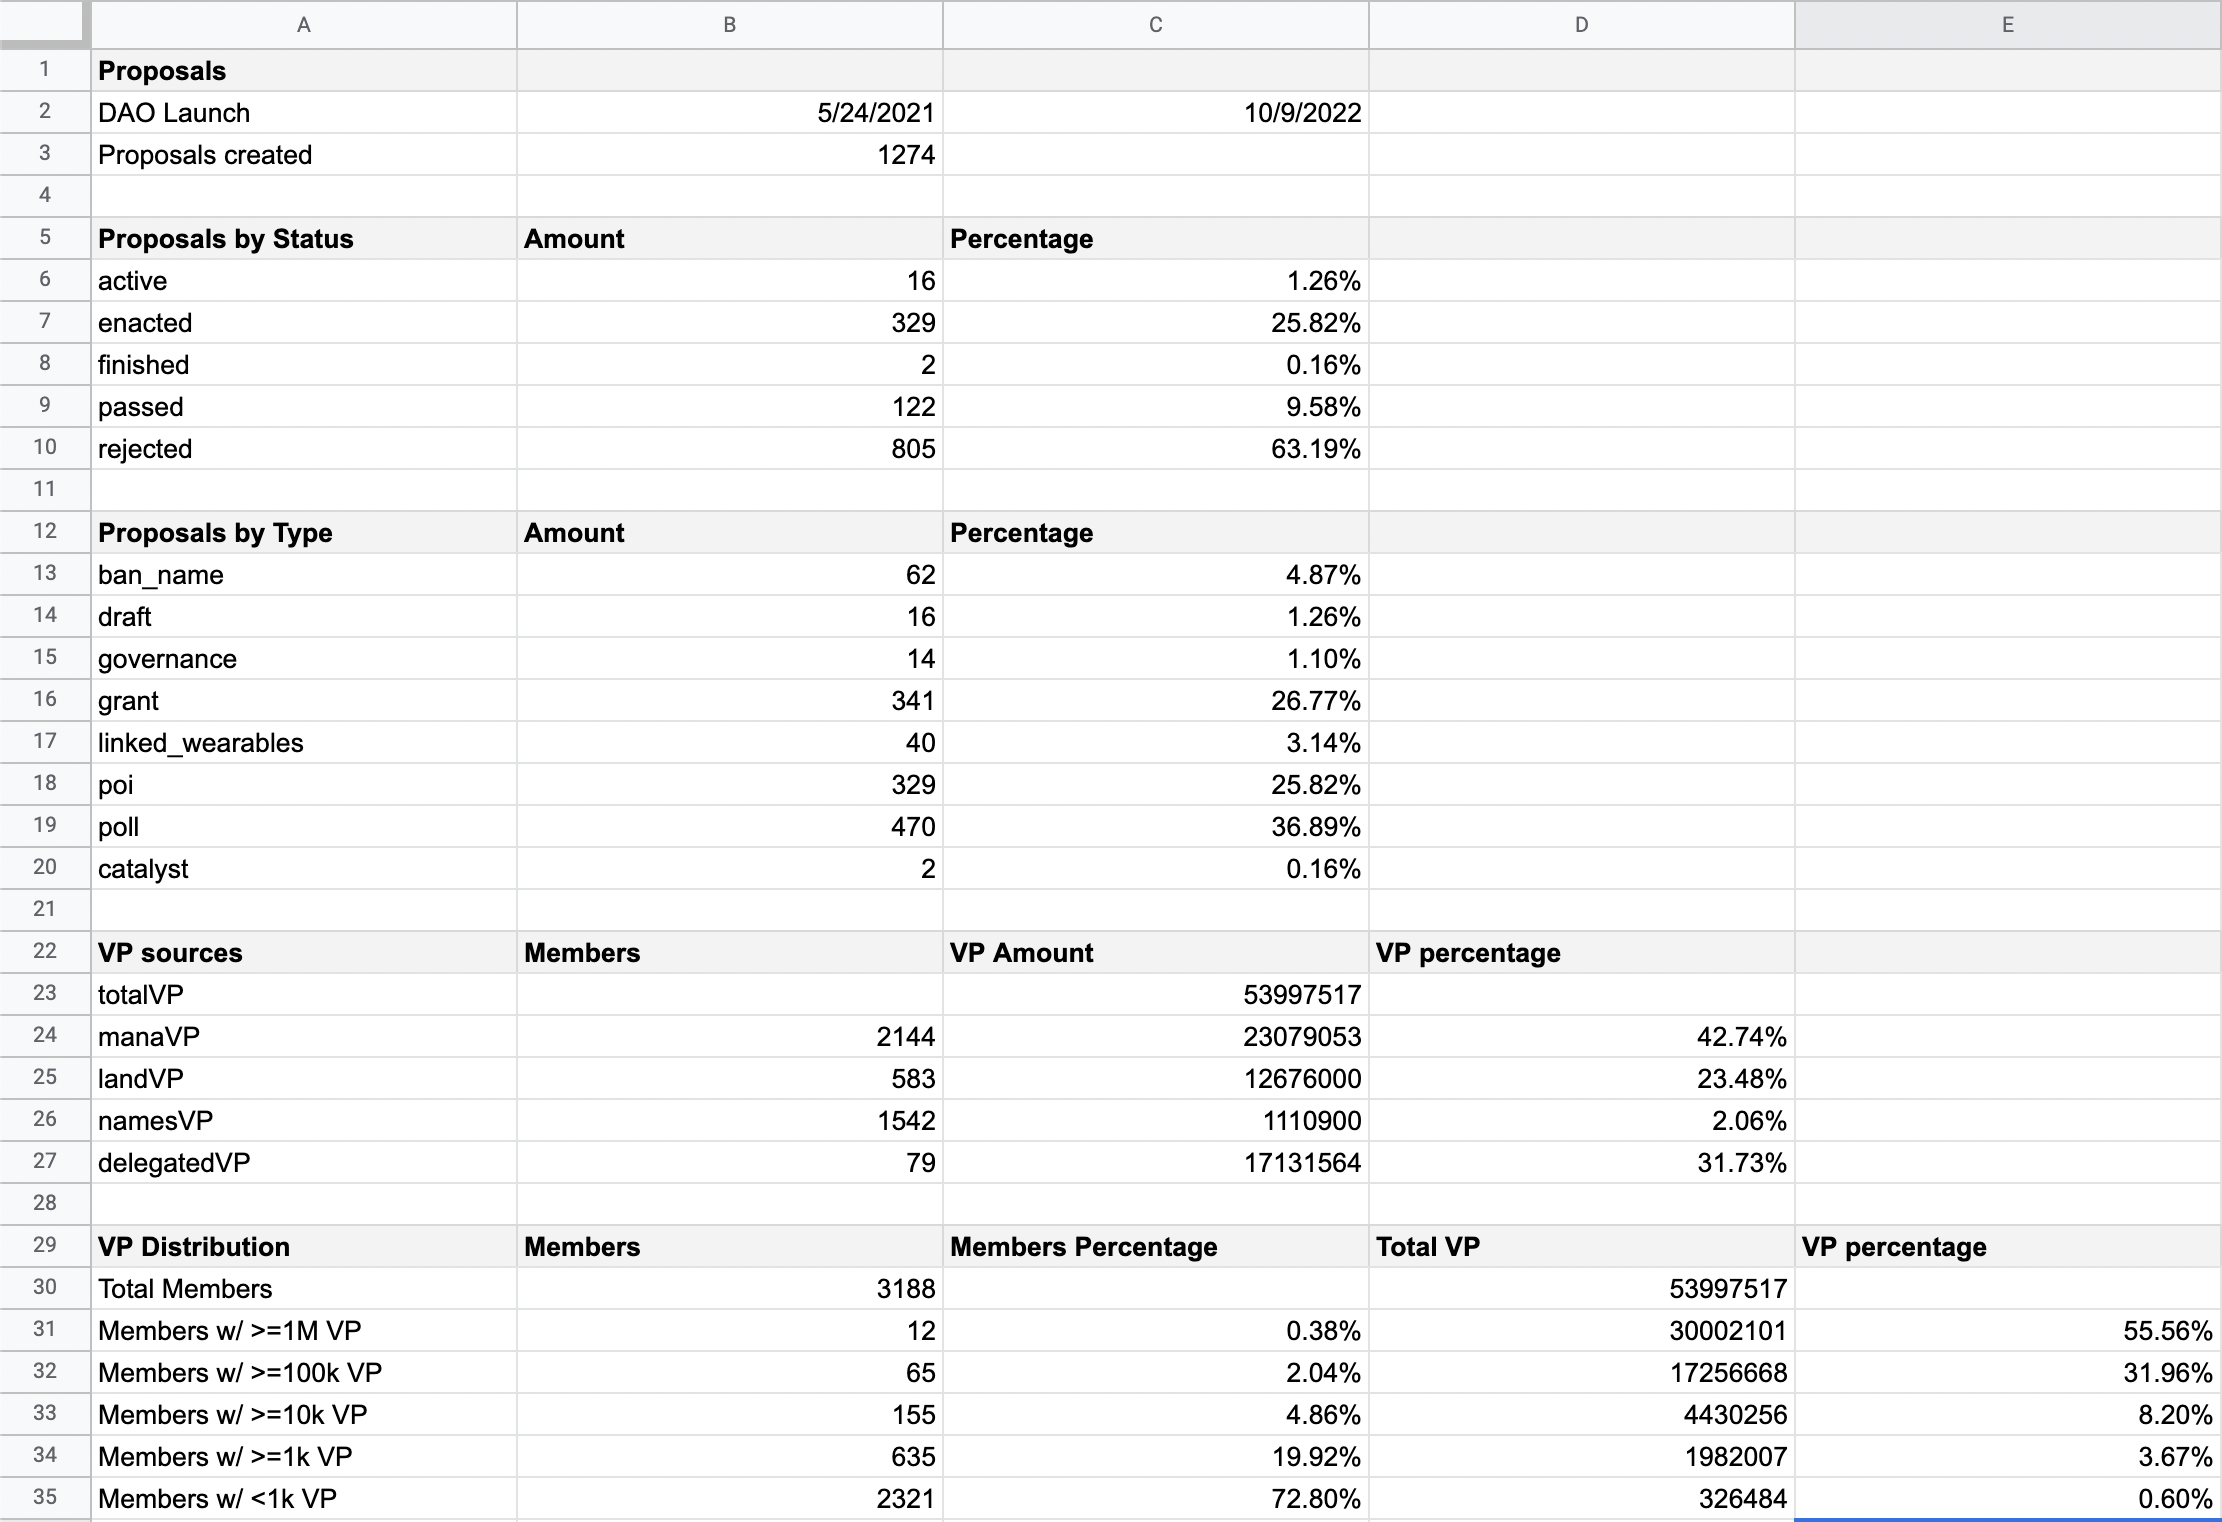
\includegraphics[width=\textwidth]{kpis.png}
  \caption{Screenshot of some KPIs}
  \label{fig:kpis}
\end{figure}

\pagebreak

Continuing with the explanation of the data flow in figure \ref{fig:diagram}, such scripts are periodically executed from a GitHub Action and the configuration file\footnote{\url{https://github.com/Decentraland-DAO/transparency/blob/main/.github/workflows/pull-data.yml}} is as follows: \\

\begin{lstlisting}{Code snippet from the Github Action configuration file}
name: Pull Data

on:
  schedule:
    - cron: "0 10 * * *"
  workflow_dispatch:
    inputs:
      choice:
        type: choice
        description: Select fetch type
        options:
        - reduced
        - full
        default: full

jobs:
  export:
    runs-on: ubuntu-latest
    steps:
      - uses: actions/checkout@v2
      - uses: actions/setup-node@v2
        with:
          node-version: '14'
      - run: npm install && npm link typescript

      - name: Pull Proposals
        env:
          SHEET_ID: ${{ secrets.SHEET_ID }}
          SHEET_CLIENT_EMAIL: ${{ secrets.SHEET_CLIENT_EMAIL }}
          SHEET_PRIVATE_KEY: ${{ secrets.SHEET_PRIVATE_KEY }}
        run: |
          npx ts-node ./src/export-proposals.ts
          npx ts-node ./src/upload.ts Proposals ./public/proposals.csv

                    ************ Other Scripts ************
\end{lstlisting}

The resulting JSON and CSV files, on one hand are uploaded to another branch of the same github repository to make them available for being consumed and also for versioning. On the other hand, the CSV files are uploaded to a Google spreadsheet\footnote{\url{https://docs.google.com/spreadsheets/d/1FoV7TdMTVnqVOZoV4bvVdHWkeu4sMH5JEhp8L0Shjlo}} to offer the possibility to filter the information and to make it available for use in Google Data Studio.

At this point, the data is used to extract metrics and plot them on the Data Studio dashboard, the DAO transparency page\footnote{\url{https://governance.decentraland.org/transparency/}} and other external applications.

\section{Data visualization}
Data visualization\cite{dataviz} is the representation of data through use of common graphics, such as charts, plots, infographics, and even animations. These visual displays of information communicate complex data relationships and data-driven insights in a way that is easy to understand.

It can be utilized for a variety of purposes, and it's important to note that is not only reserved for use by data teams. Management also leverages it to convey organizational structure and hierarchy while data analysts and data scientists use it to discover and explain patterns and trends. Harvard Business Review\cite{hbr} categorizes data visualization into four key purposes: idea generation, idea illustration, visual discovery, and everyday dataviz. These are described in more detail below:

\subsubsection{Idea generation}
Data visualization is commonly used to spur idea generation across teams. They are frequently leveraged during brainstorming or Design Thinking sessions at the start of a project by supporting the collection of different perspectives and highlighting the common concerns of the collective. While these visualizations are usually unpolished and unrefined, they help set the foundation within the project to ensure that the team is aligned on the problem that they're looking to address for key stakeholders.

\subsubsection{Idea illustration}
Data visualization for idea illustration assists in conveying an idea, such as a tactic or process. It is commonly used in learning settings, such as tutorials, certification courses, centers of excellence, but it can also be used to represent organization structures or processes, facilitating communication between the right individuals for specific tasks. Project managers frequently use Gantt charts and waterfall charts to illustrate workflows. Data modeling also uses abstraction to represent and better understand data flow within an enterprise's information system, making it easier for developers, business analysts, data architects, and others to understand the relationships in a database or data warehouse.

\subsubsection{Visual discovery}
Visual discovery and every day data viz are more closely aligned with data teams. While visual discovery helps data analysts, data scientists, and other data professionals identify patterns and trends within a dataset, every day data viz supports the subsequent storytelling after a new insight has been found.

\section{Types of data visualizations}
The earliest form of data visualization can be traced back the Egyptians in the pre-17th century\cite{dataviz}, largely used to assist in navigation. As time progressed, people leveraged data visualizations for broader applications, such as in economic, social, health disciplines. Perhaps most notably, Edward Tufte published The Visual Display of Quantitative Information\cite{tufte1985visual}, which illustrated that individuals could utilize data visualization to present data in a more effective manner. Dashboards are effective data visualization tools for tracking and visualizing data from multiple data sources, providing visibility into the effects of specific behaviors by a team or an adjacent one on performance. Dashboards include common visualization techniques, such as:

\begin{itemize}
  \item \textbf{Tables}: This consists of rows and columns used to compare variables. Tables can show a great deal of information in a structured way, but they can also overwhelm users that are simply looking for high-level trends.
  \item \textbf{Pie charts and stacked bar charts}: These graphs are divided into sections that represent parts of a whole. They provide a simple way to organize data and compare the size of each component to one other.
  \item \textbf{Line charts and area charts}: These visuals show change in one or more quantities by plotting a series of data points over time and are frequently used within predictive analytics. Line graphs utilize lines to demonstrate these changes while area charts connect data points with line segments, stacking variables on top of one another and using color to distinguish between variables.
  \item \textbf{Histograms}: This graph plots a distribution of numbers using a bar chart (with no spaces between the bars), representing the quantity of data that falls within a particular range. This visual makes it easy for an end user to identify outliers within a given dataset.
  \item \textbf{Scatter plots}: These visuals are beneficial in reveling the relationship between two variables, and they are commonly used within regression data analysis. However, these can sometimes be confused with bubble charts, which are used to visualize three variables via the x-axis, the y-axis, and the size of the bubble.
  \item \textbf{Heat maps}: These graphical representation displays are helpful in visualizing behavioral data by location. This can be a location on a map, or even a webpage.
  \item \textbf{Tree maps}: They display hierarchical data as a set of nested shapes, typically rectangles. Treemaps are great for comparing the proportions between categories via their area size.
\end{itemize}

\chapter{Discussion\label{discussion}}
The visualizations of the metrics that resulted from the data collected will be presented below. These are divided into the categories: Proposals, Voting Power, Grants, DAO Balances, Wearable Curations and DAO Members. The analysis period will be 12 months and will run from October 2021 to September 2022, unless otherwise clarified.

\section{Proposals}
Figure \ref{fig:proposal_types} shows the number of proposals created according to their category, being surveys, grants and points of interest the most frequents.
\begin{figure}[H]
  \centering
  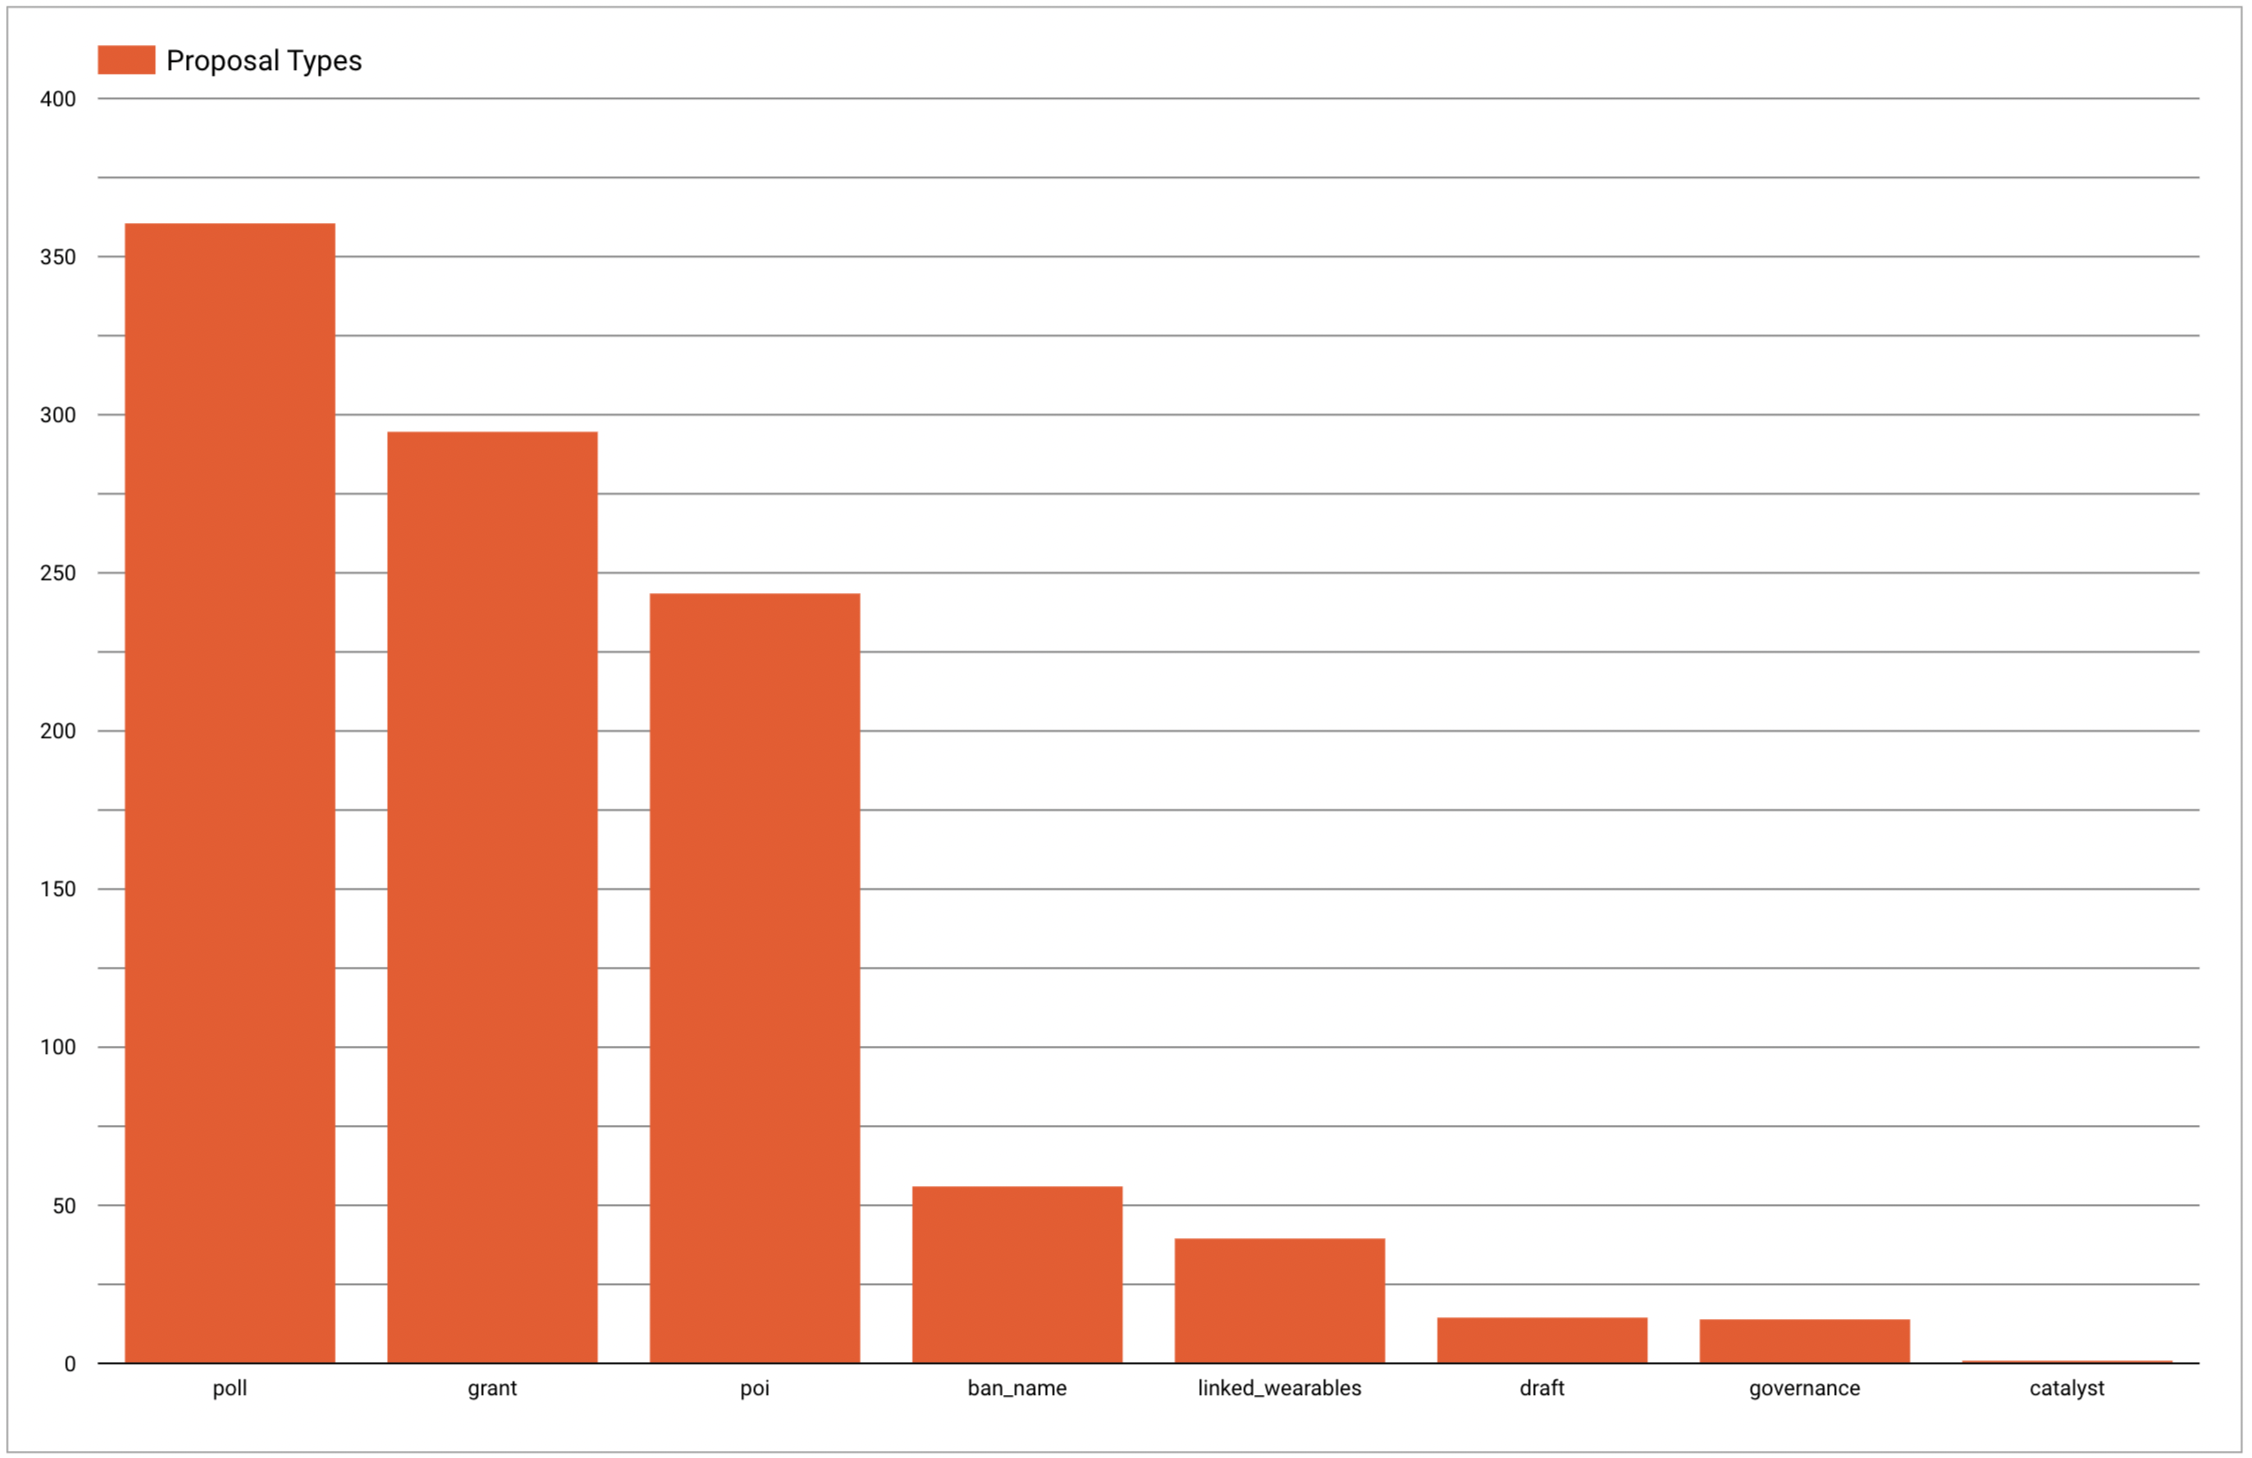
\includegraphics[width=\textwidth]{metrics/proposal_types.png}
  \caption{Amount of proposals created according to their category}
  \label{fig:proposal_types}
\end{figure}

Figure \ref{fig:proposal_status} shows the final result of the proposals once the voting period is over, where 66\% are rejected, 25\% are enacted and 8\% are approved.
\begin{figure}[H]
  \centering
  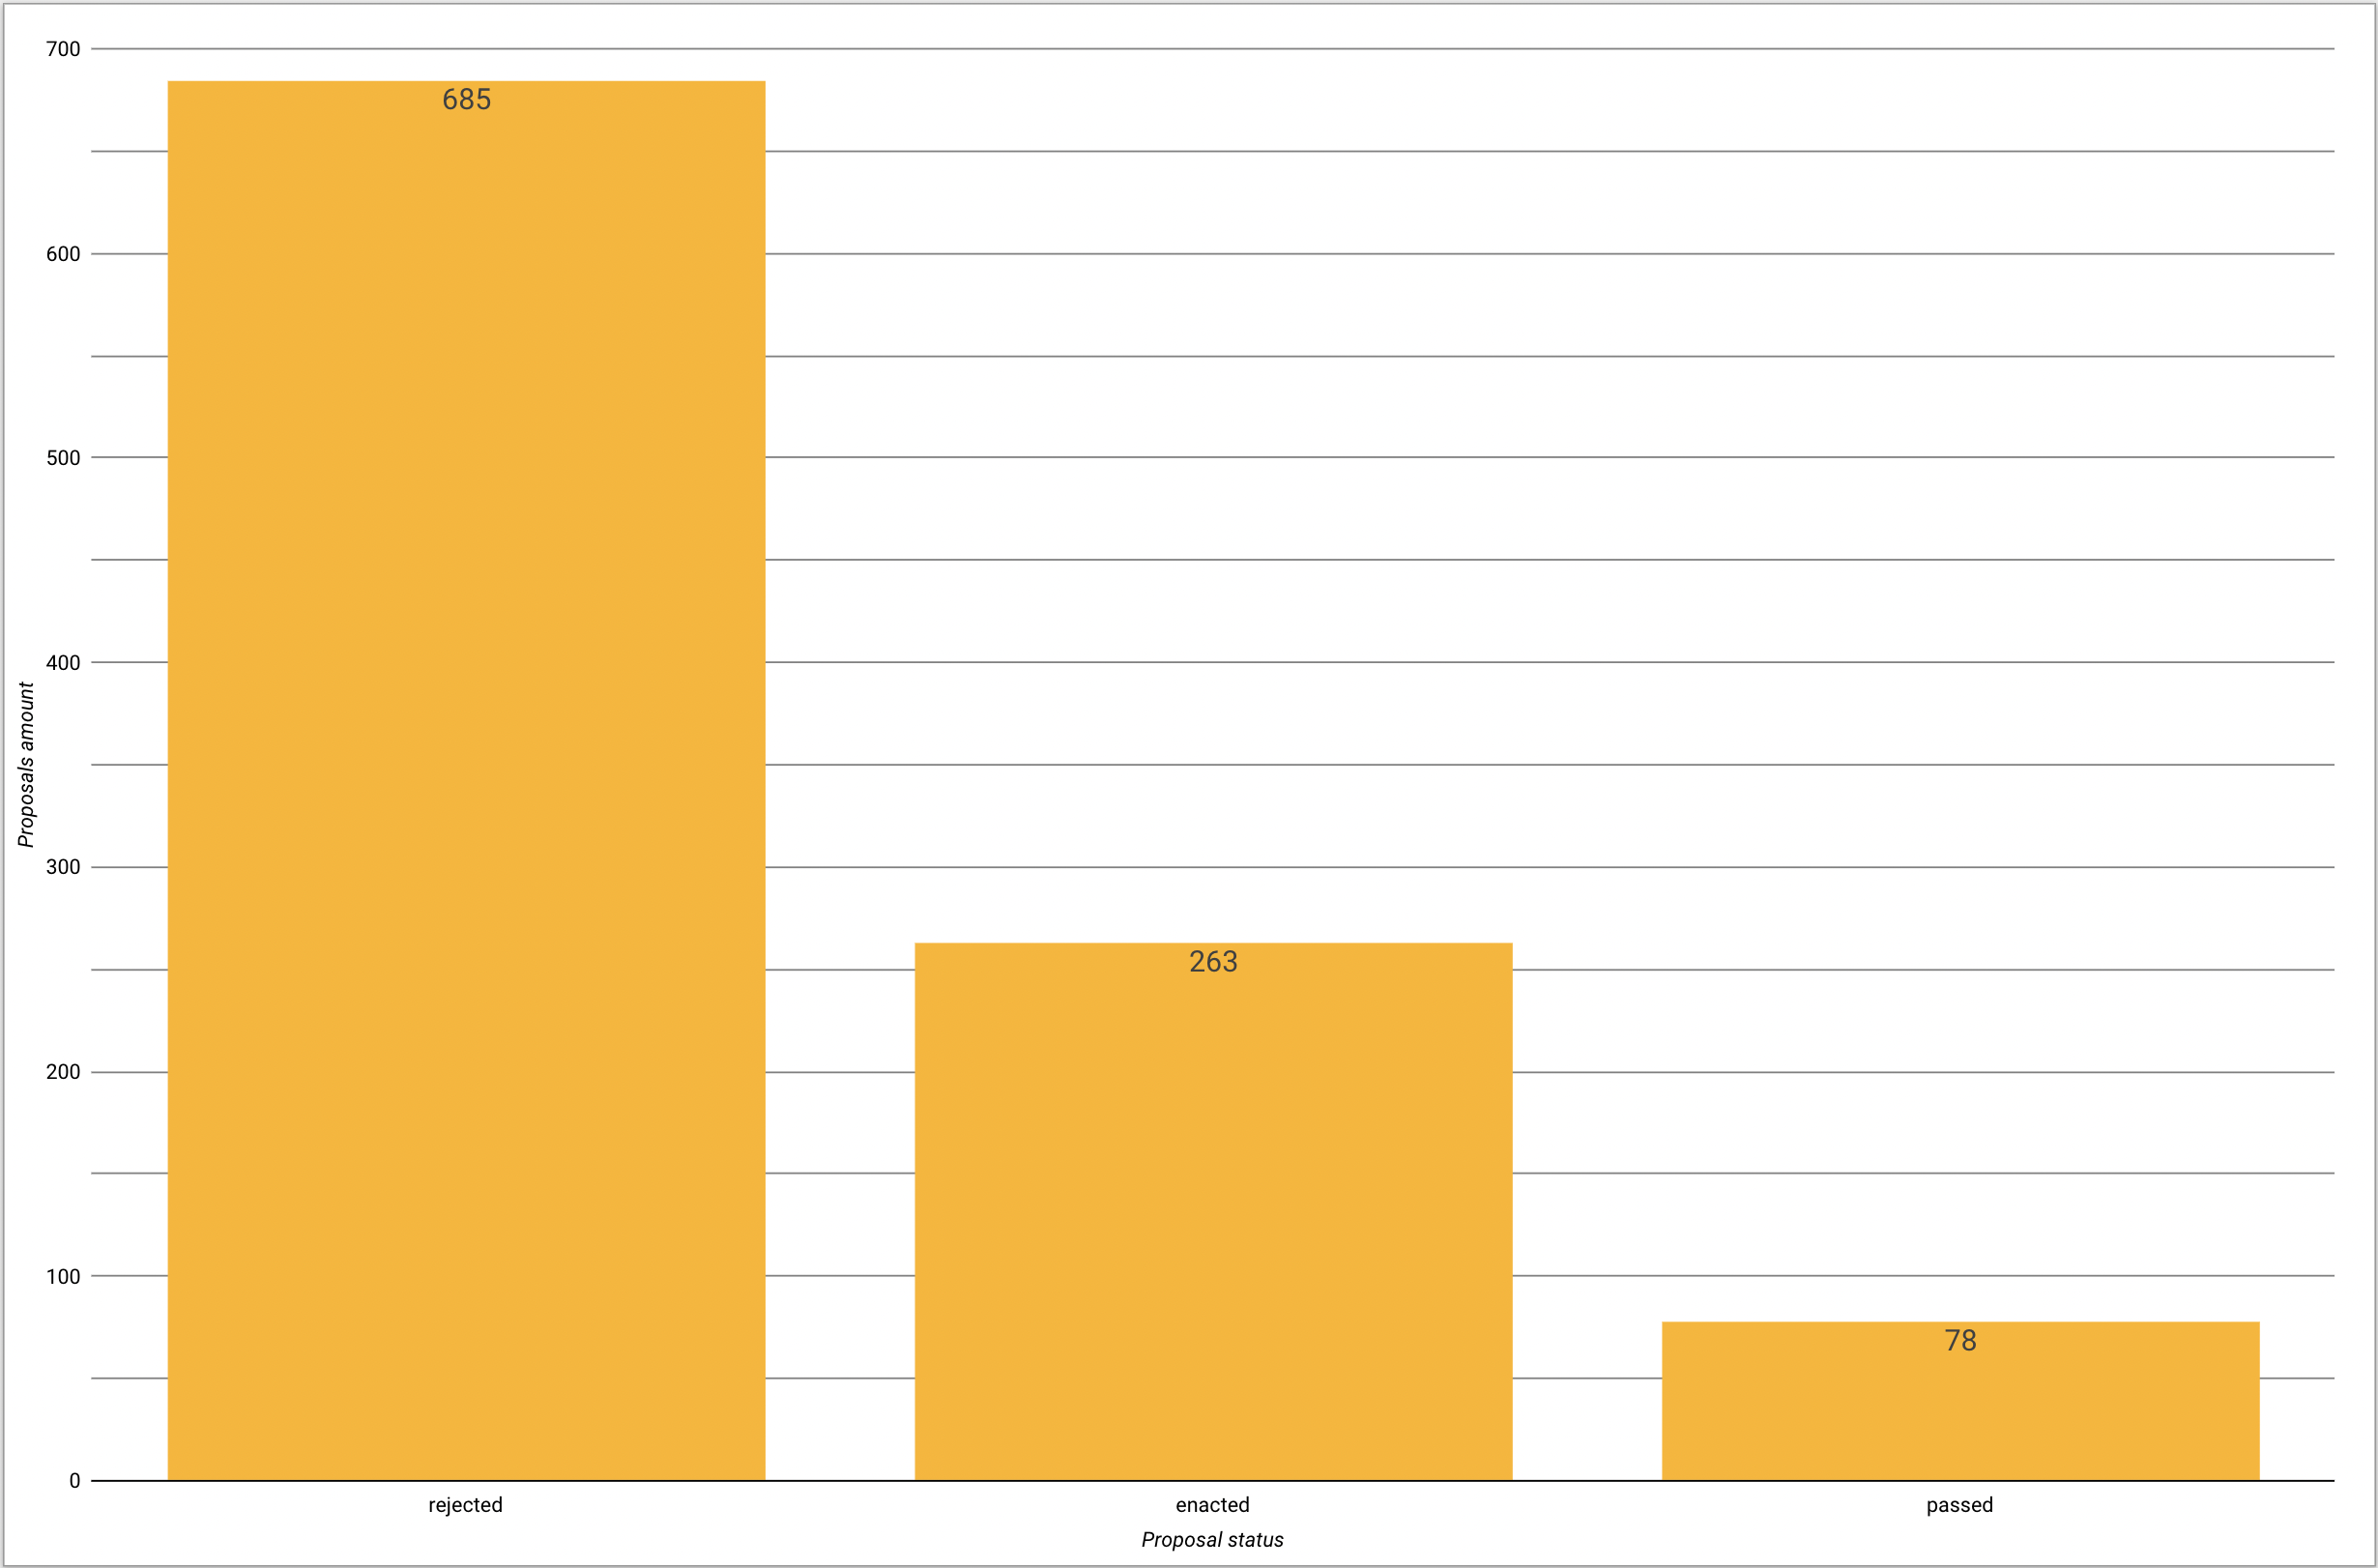
\includegraphics[width=\textwidth]{metrics/proposal_status.png}
  \caption{Status of proposals after the voting period}
  \label{fig:proposal_status}
\end{figure}

Figure \ref{fig:proposals_by_month} shows the proposals created per month by category. It can be observed, on the one hand, that there is a constant number of grant requests and points of interest and, on the other hand, that very few polls become draft and then governance proposals.
\begin{figure}[H]
  \centering
  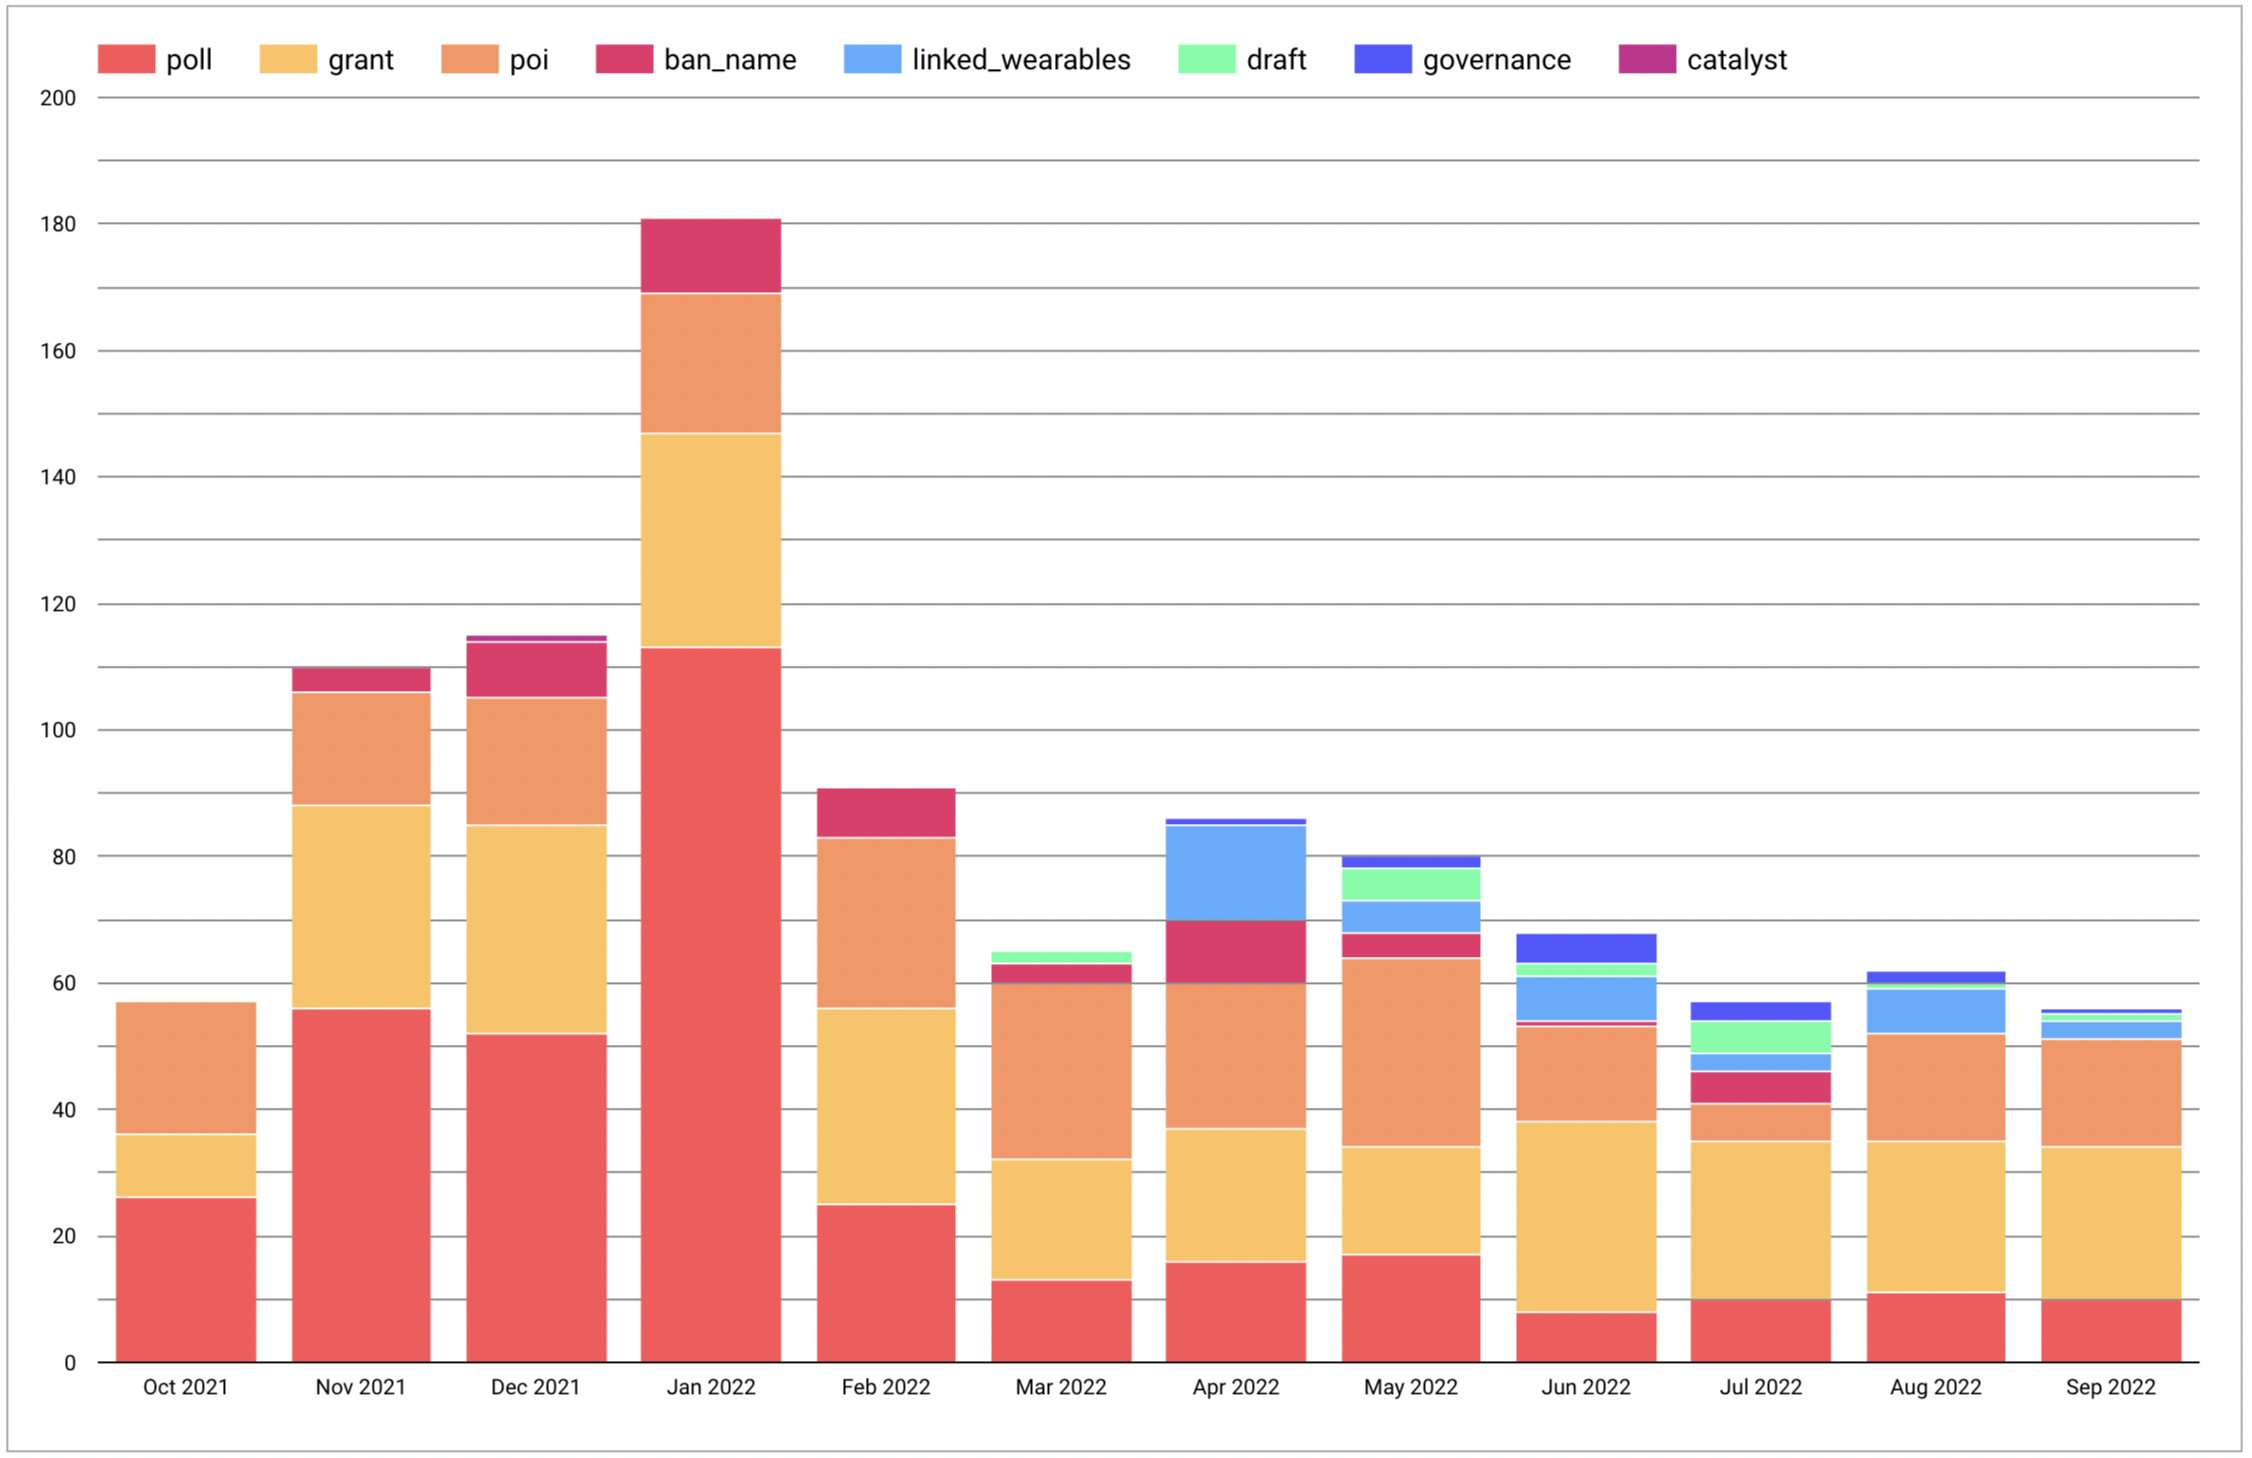
\includegraphics[width=\textwidth]{metrics/proposals_by_month.png}
  \caption{Number of proposals created per month by category}
  \label{fig:proposals_by_month}
\end{figure}

Figure \ref{fig:top_proposals} shows the historical top 25 to date of proposals ordered by total VP received, where the first has almost 15 million and the last just under 10 million.
\begin{figure}[H]
  \centering
  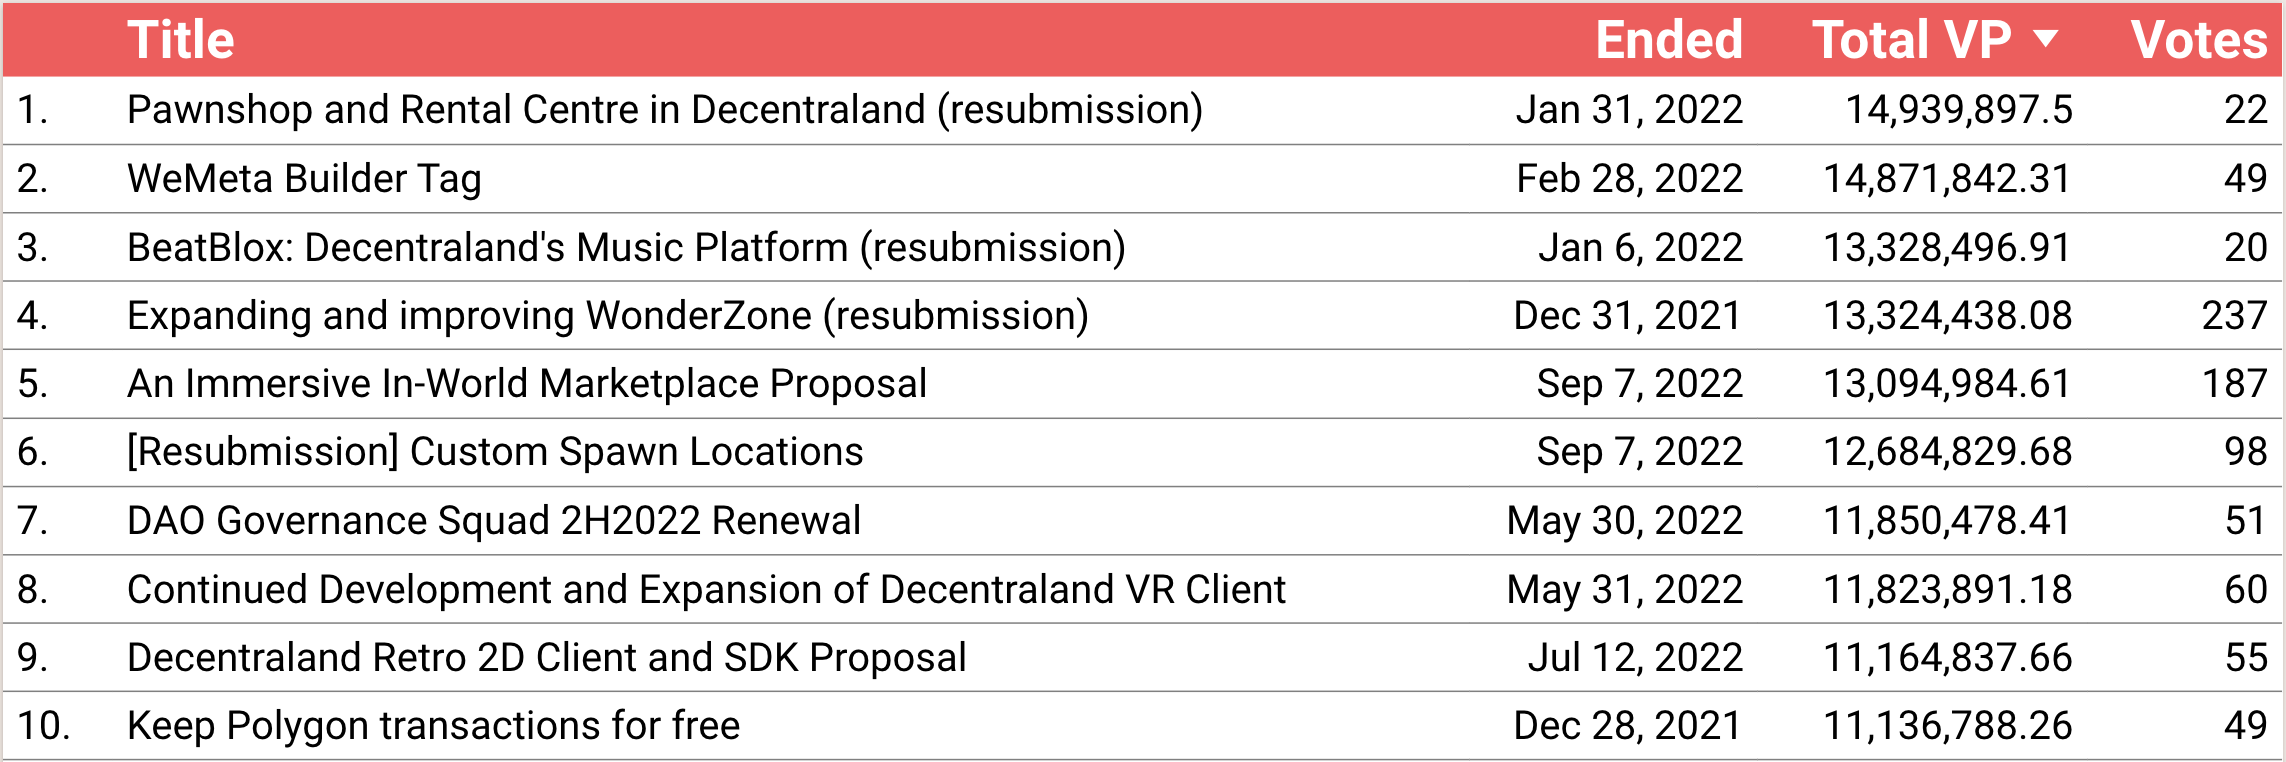
\includegraphics[width=\textwidth]{metrics/top_proposals.png}
  \caption{Top 25 historical proposals ranked by total Voting Power received}
  \label{fig:top_proposals}
\end{figure}

Finally in this section is Figure \ref{fig:median_votes} which shows the median number of votes per proposal per month where an increase in said number month to month is evident.
\begin{figure}[H]
  \centering
  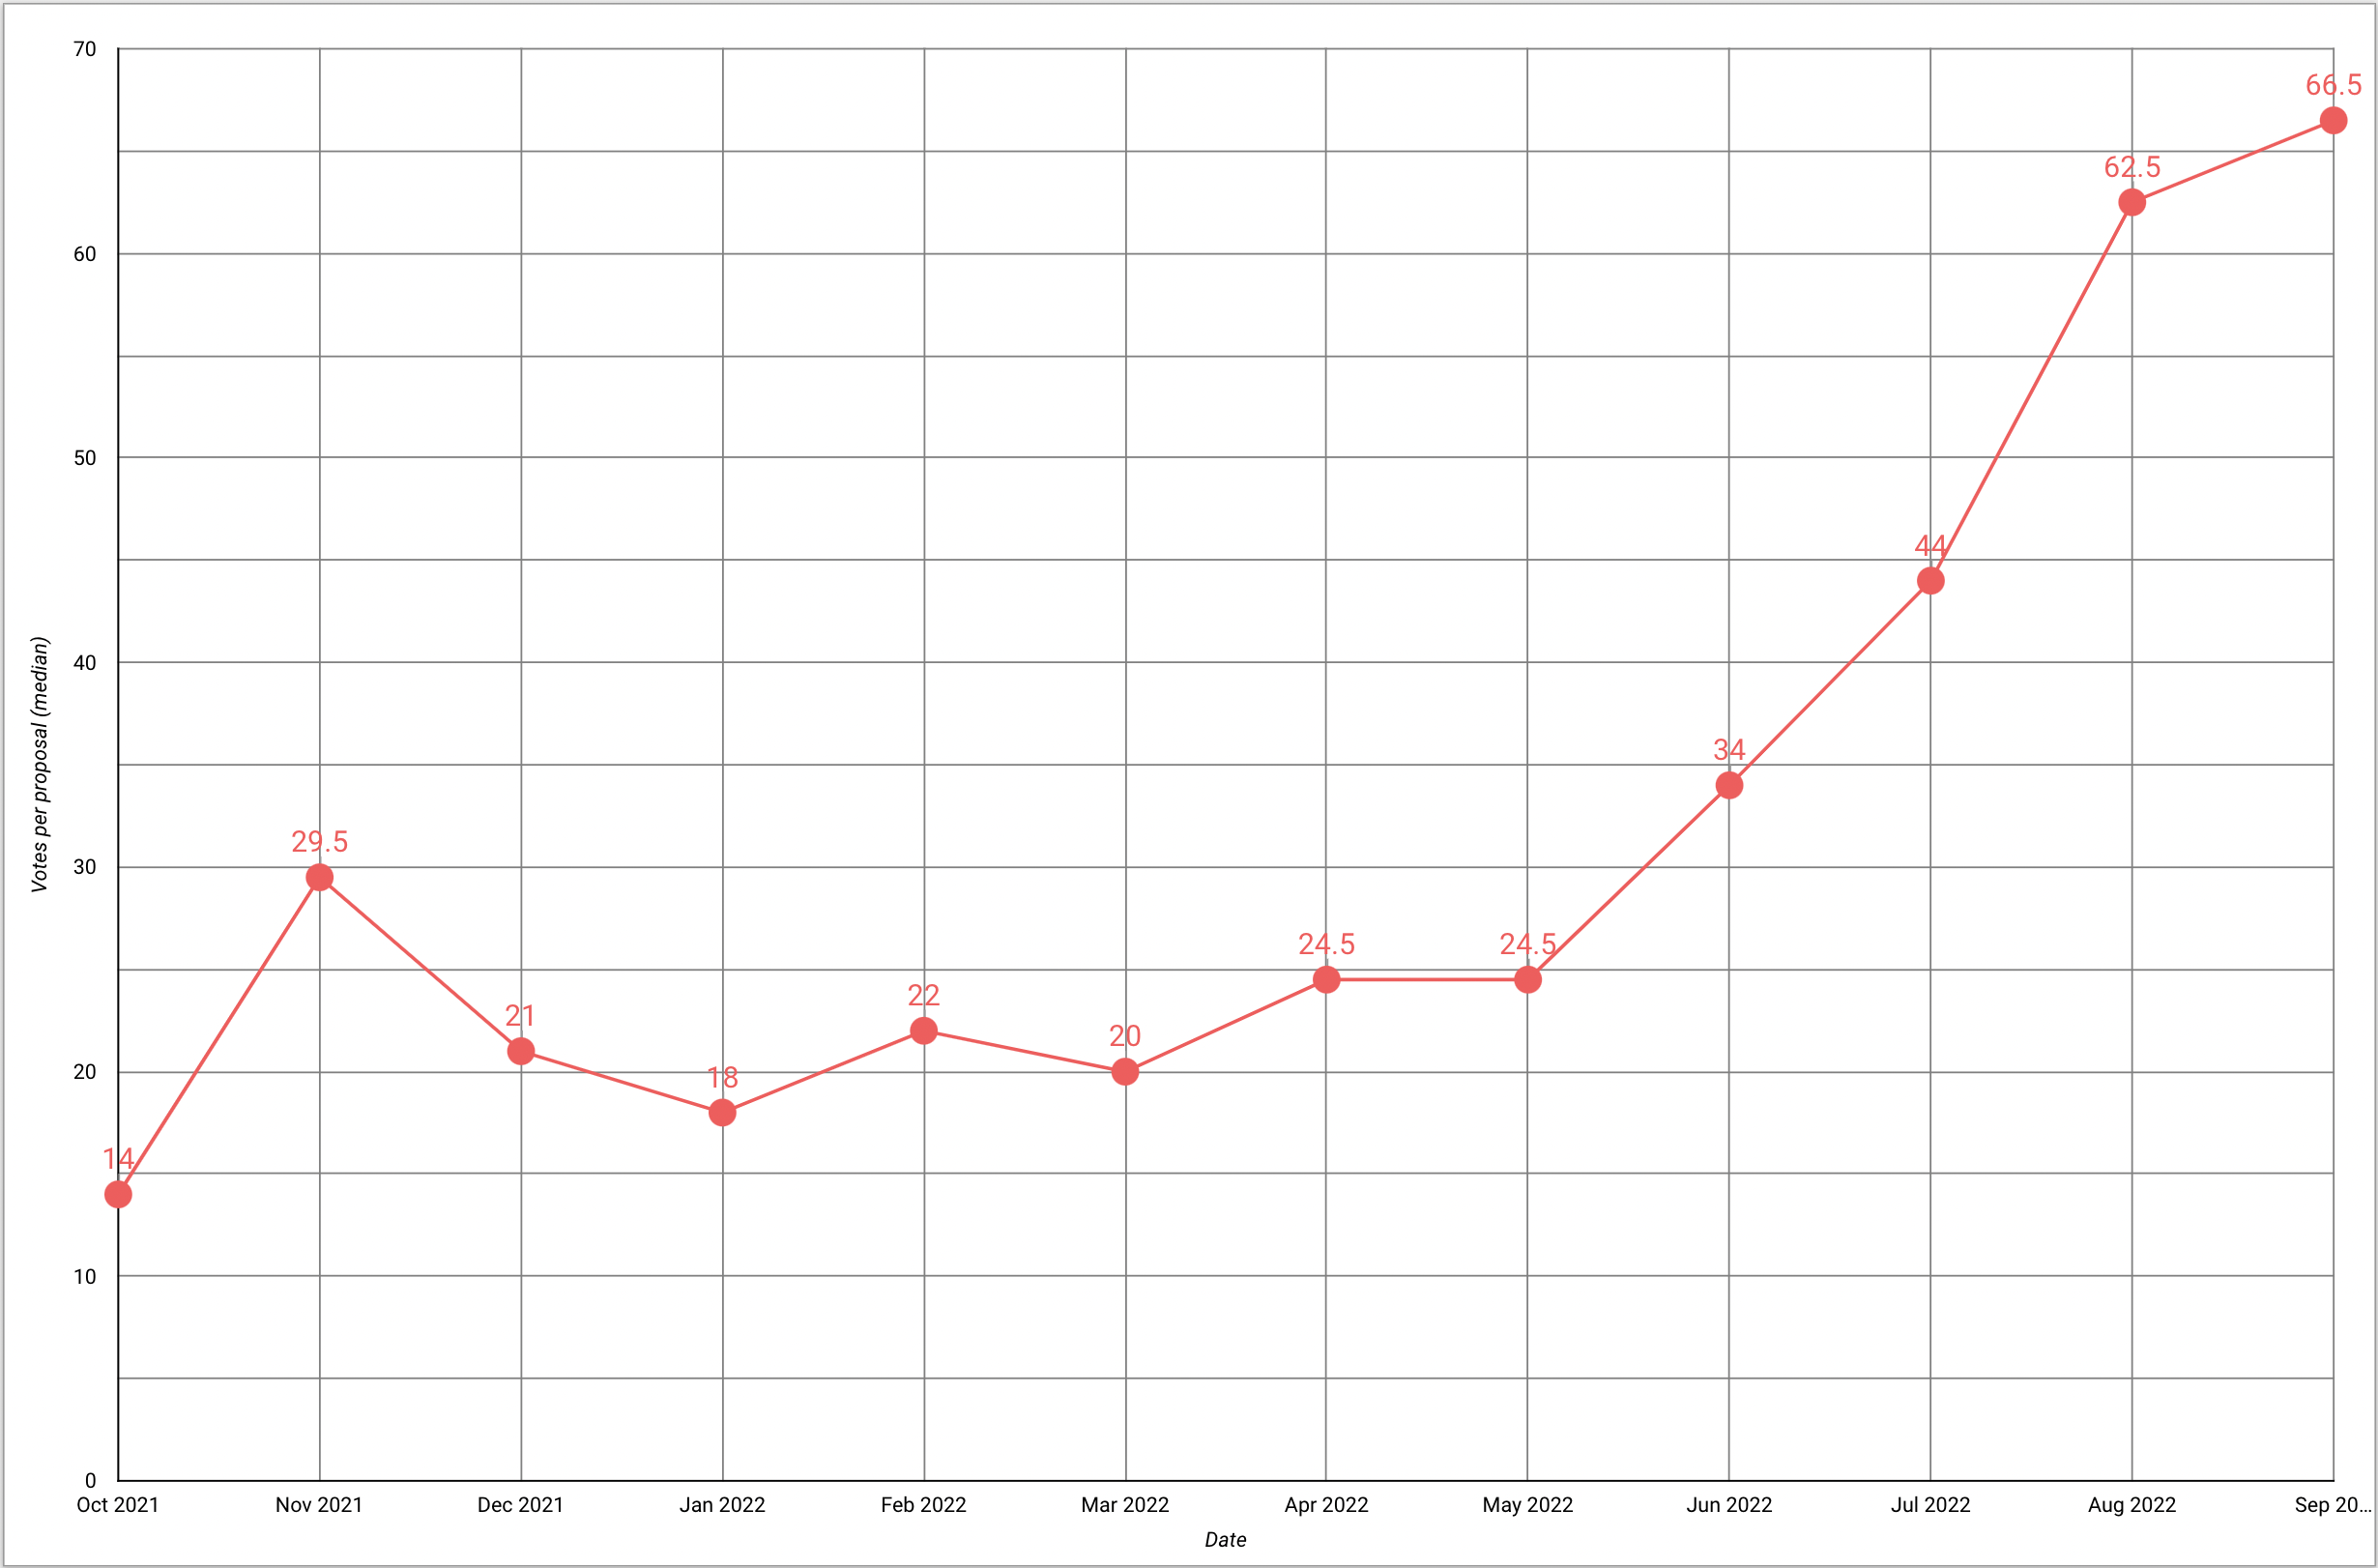
\includegraphics[width=\textwidth]{metrics/median_votes.png}
  \caption{Median votes on proposals per month}
  \label{fig:median_votes}
\end{figure}


\section{Voting Power}
\begin{center}
  \begin{table}[H]
    \begin{tabular}{ | m{20em} | m{20em} | }
      \hline
      \textbf{Total Voting Power} & \textbf{Delegated Voting Power ratio} \\
      \hline
      53.9M & 31.8\% \\
      \hline
    \end{tabular}
    \caption{Total amount of Voting Power and delegated ratio}
    \label{table:VP}
  \end{table}
\end{center}

Figure \ref{fig:vp_distribution} shows how the voting power of DAO members is distributed to date, with MANA, delegated voting power and LAND being the dominant ones.
\begin{figure}[H]
  \centering
  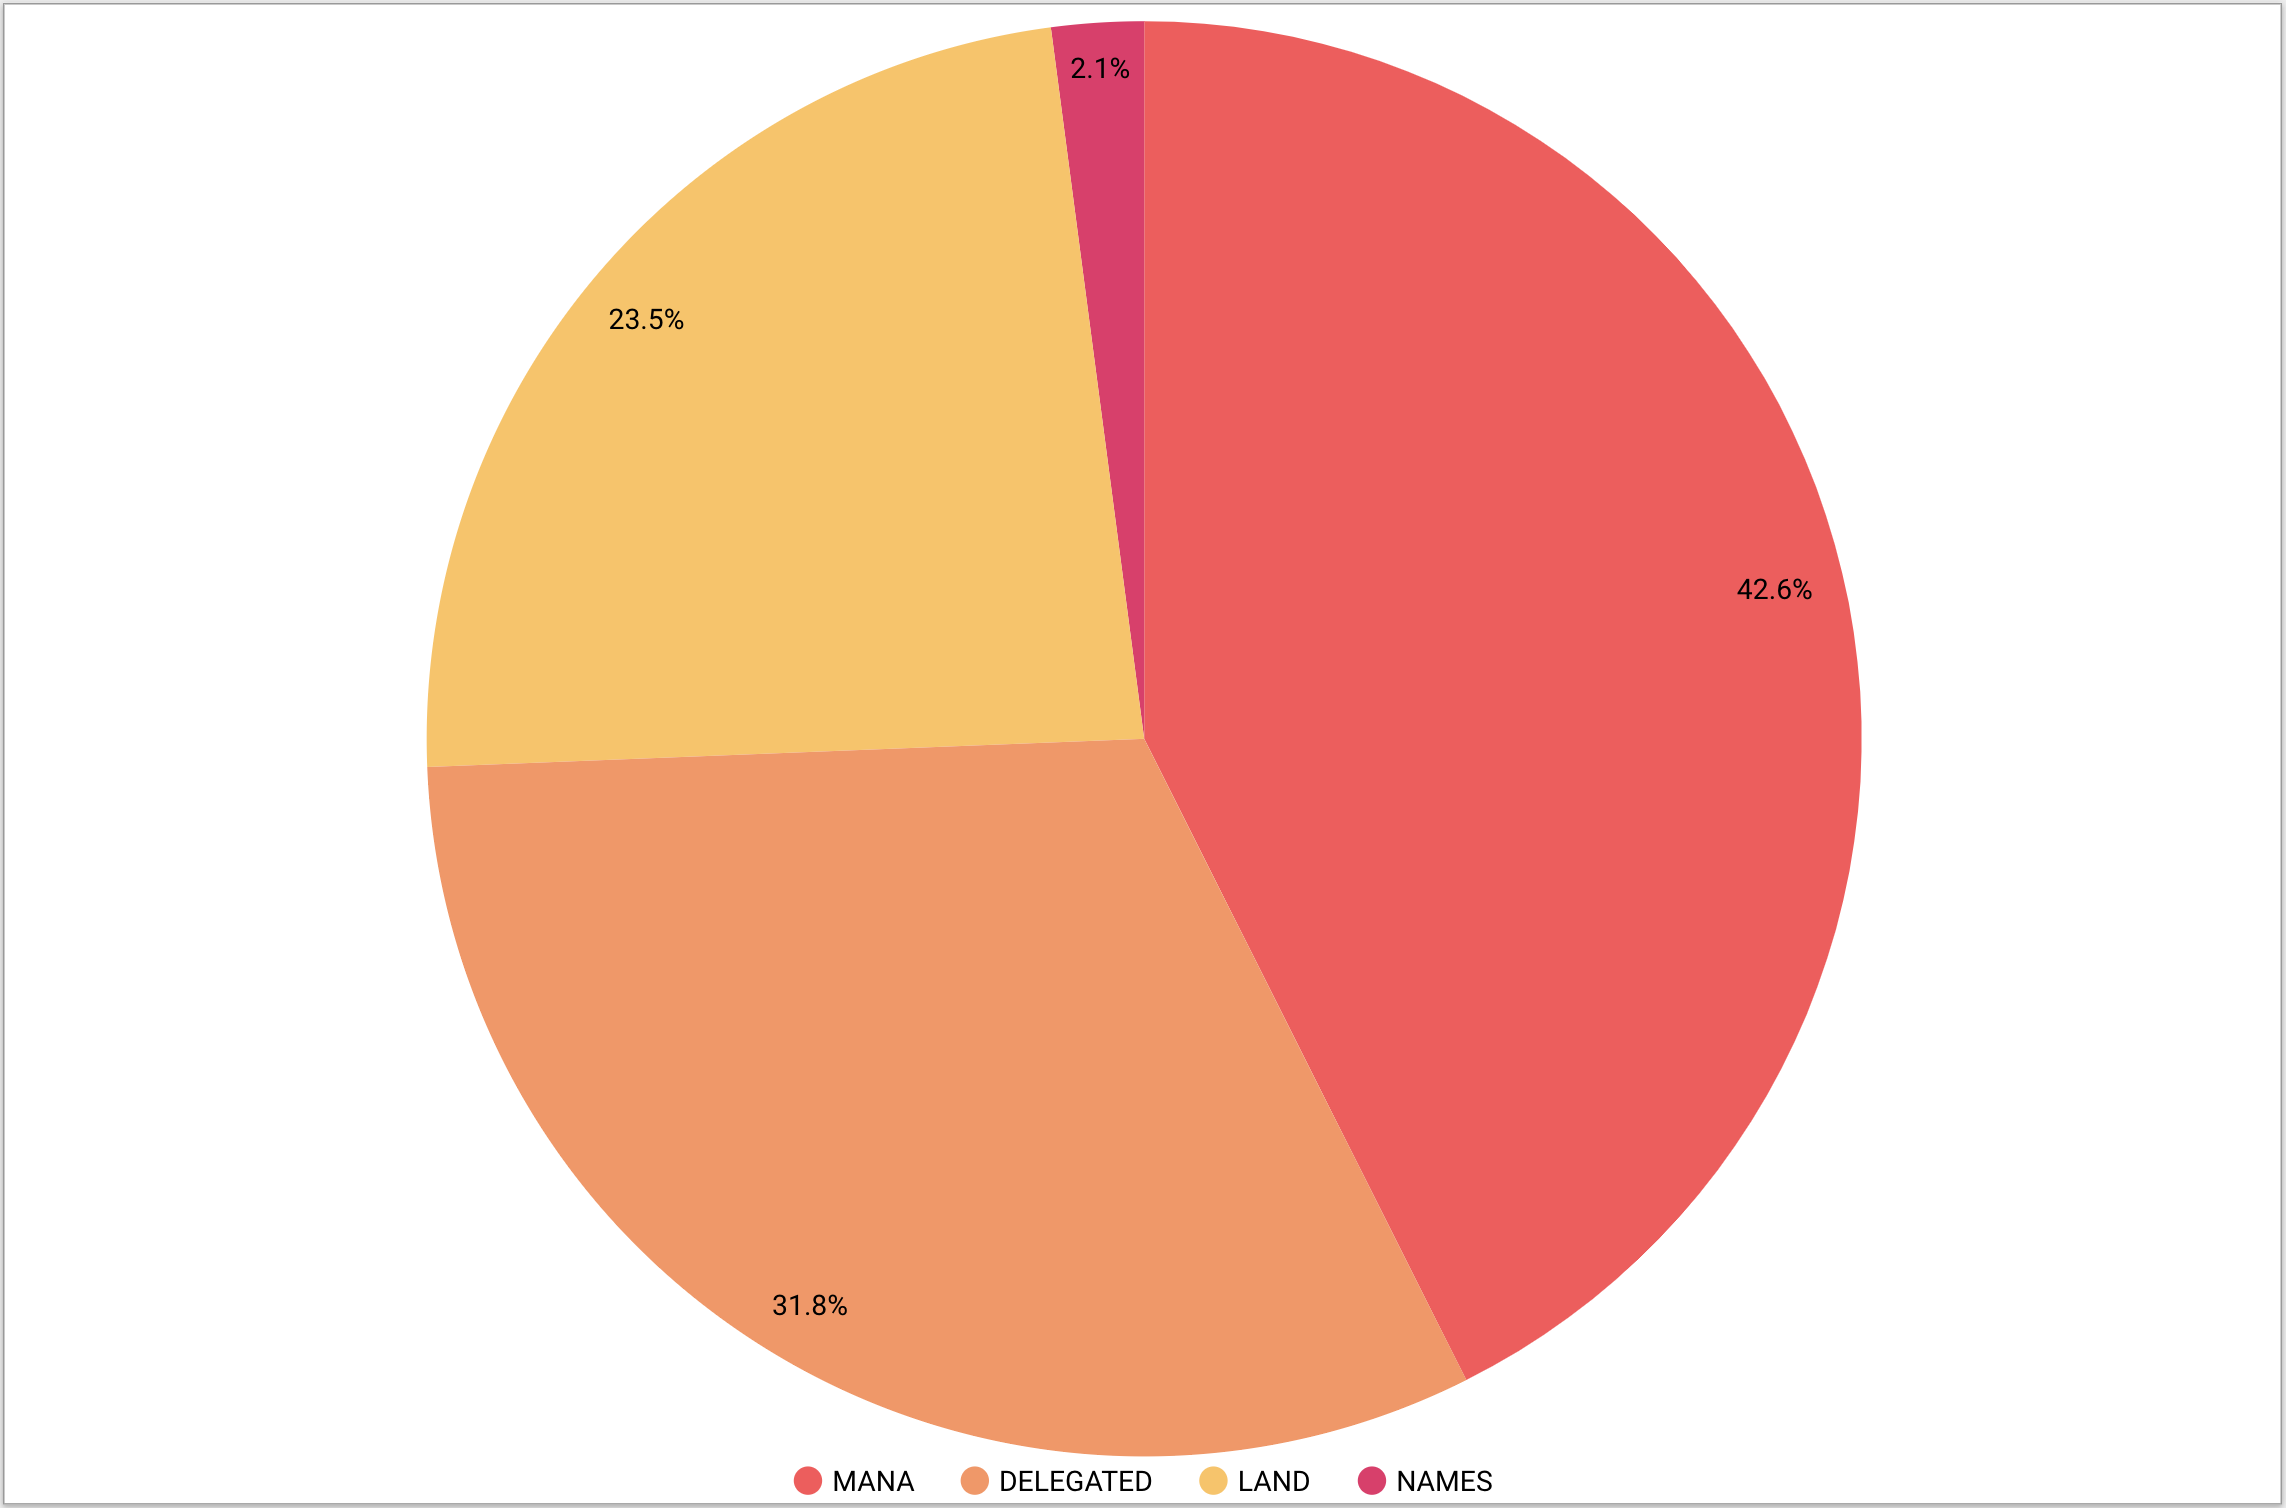
\includegraphics[width=\textwidth]{metrics/vp_distribution.png}
  \caption{Circulating Voting Power distribution to date}
  \label{fig:vp_distribution}
\end{figure}

Figure \ref{fig:votes_vp} shows how voting power breaks down in total votes by month. A rise in delegate VP, a drop in MANA VP and a steady VP of LAND and names can be seen.
\begin{figure}[H]
  \centering
  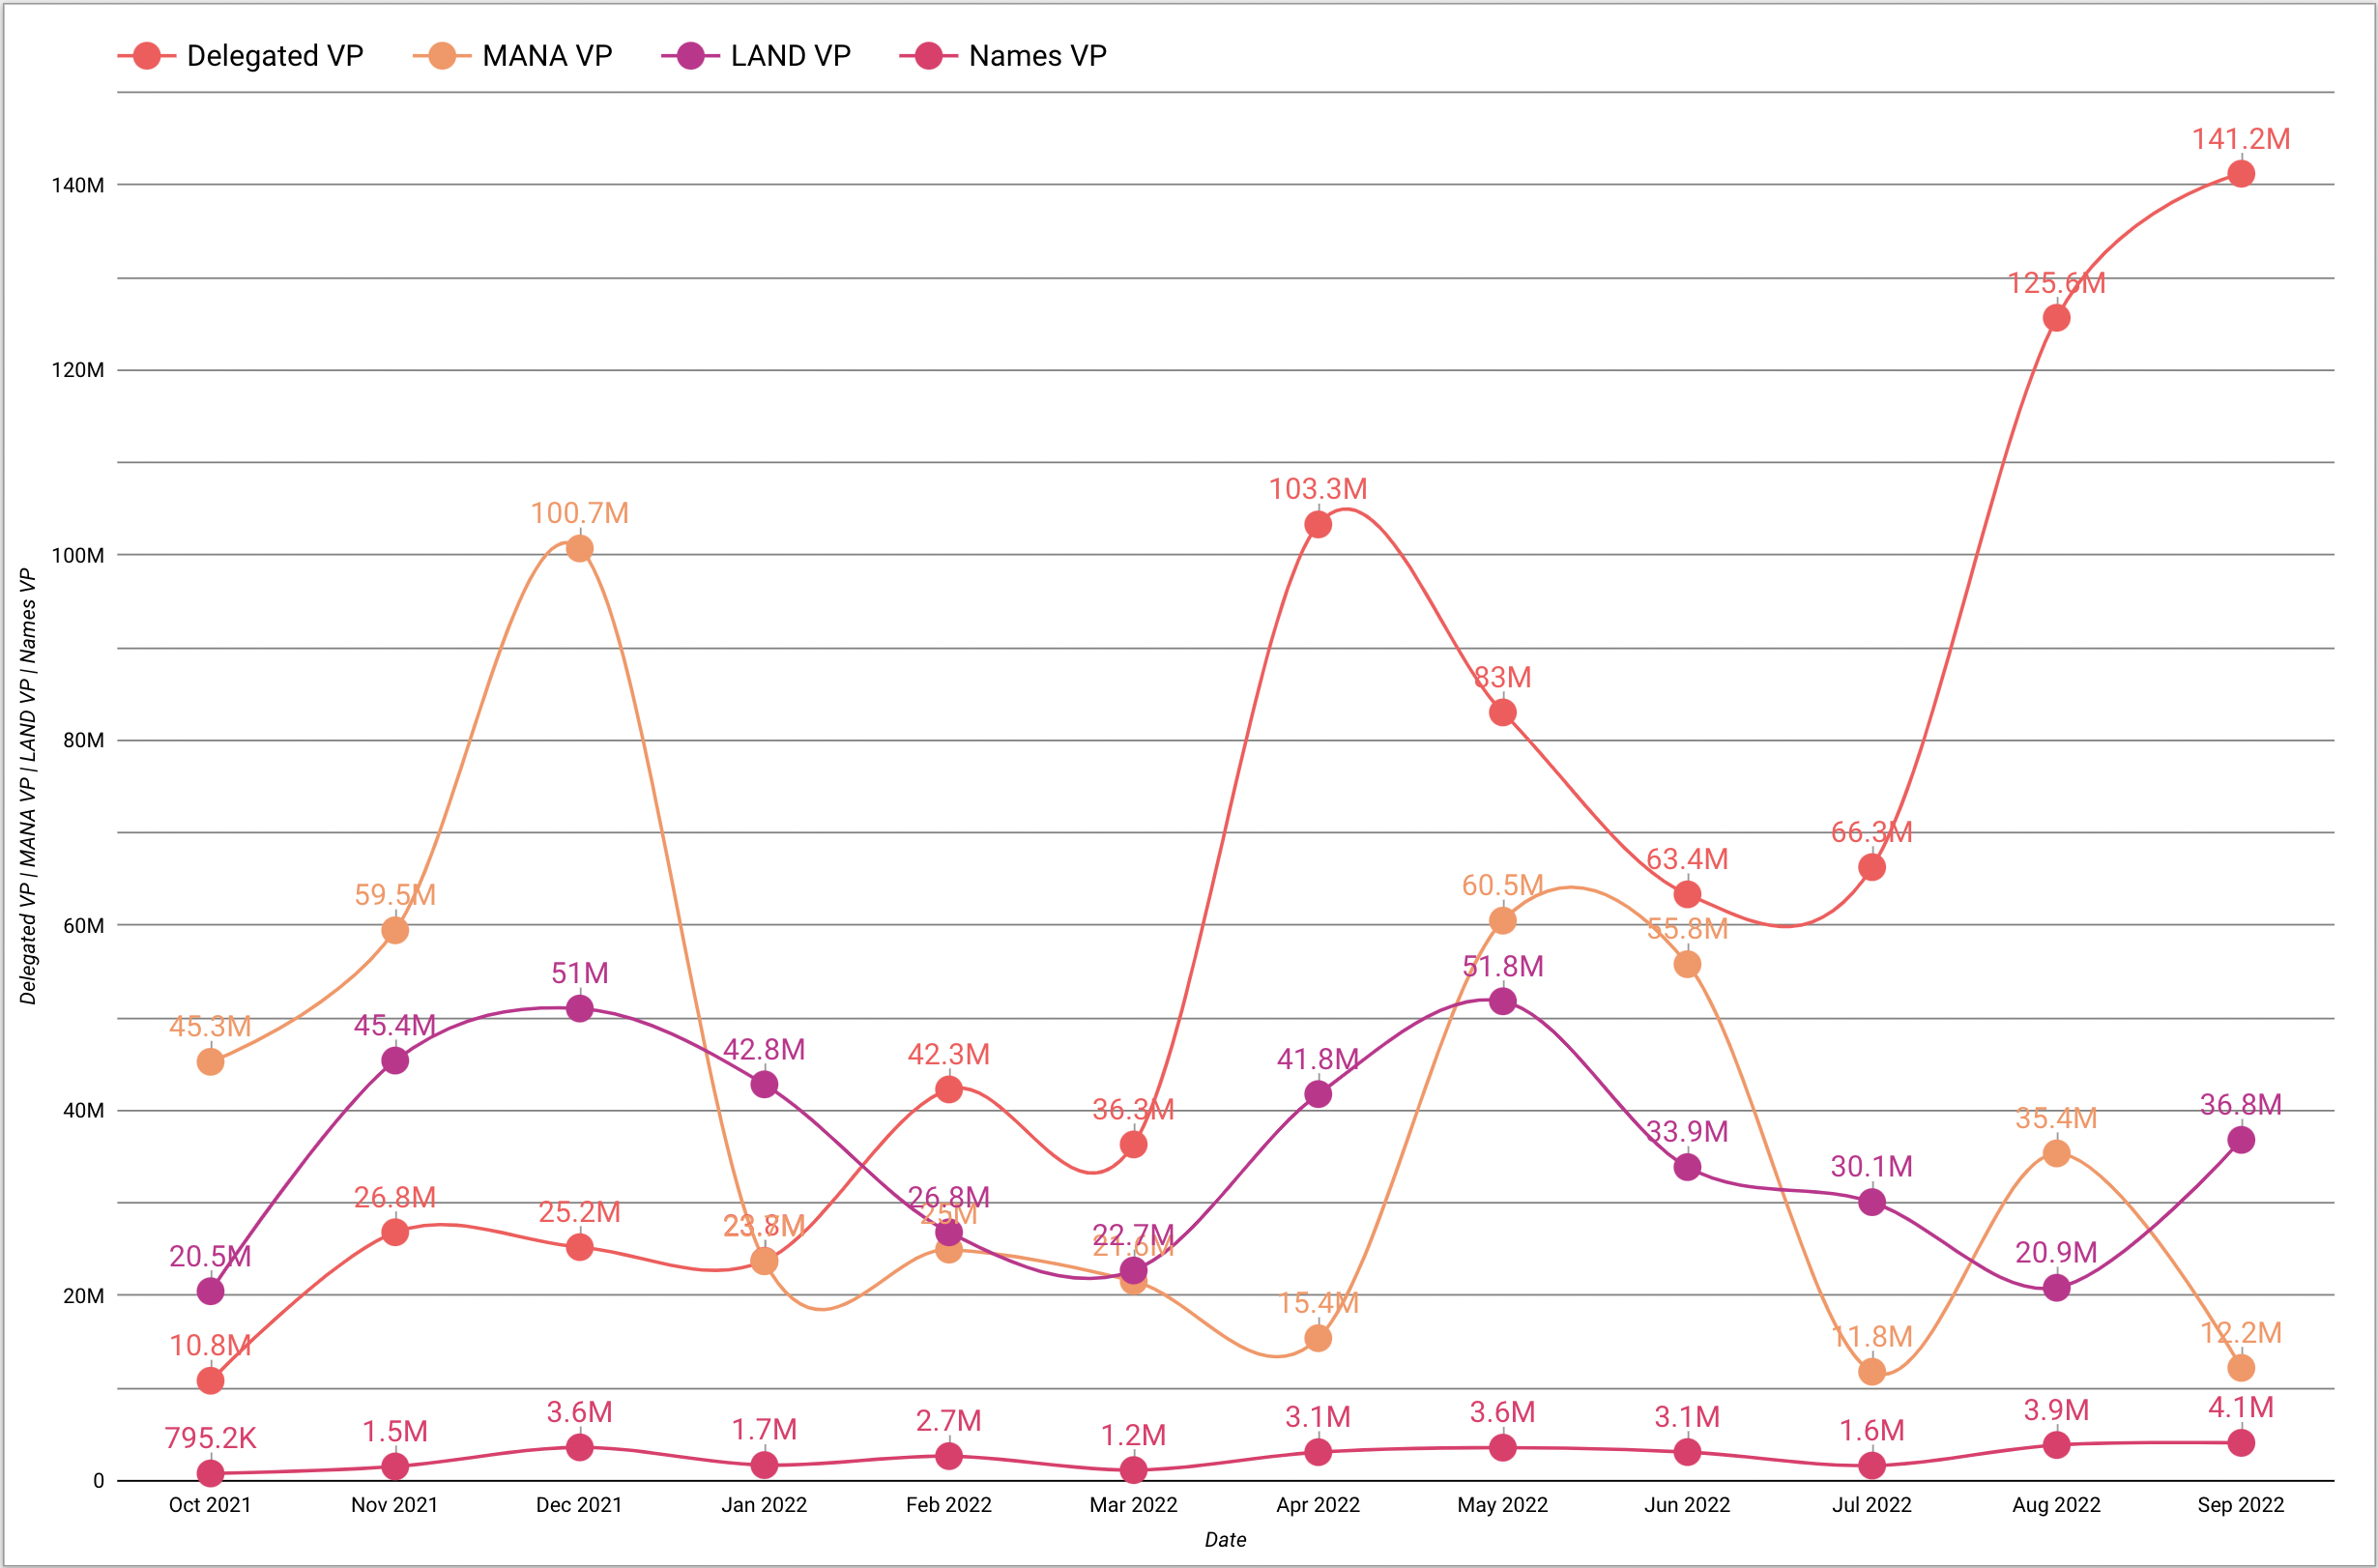
\includegraphics[width=\textwidth]{metrics/votes_breakdown.png}
  \caption{Votes VP breakdown per month}
  \label{fig:votes_vp}
\end{figure}

Figure \ref{fig:vp_distribution_members} shows how voting power is distributed among DAO members. A large concentration of VP can be seen in a few of them.
\begin{figure}[H]
  \centering
  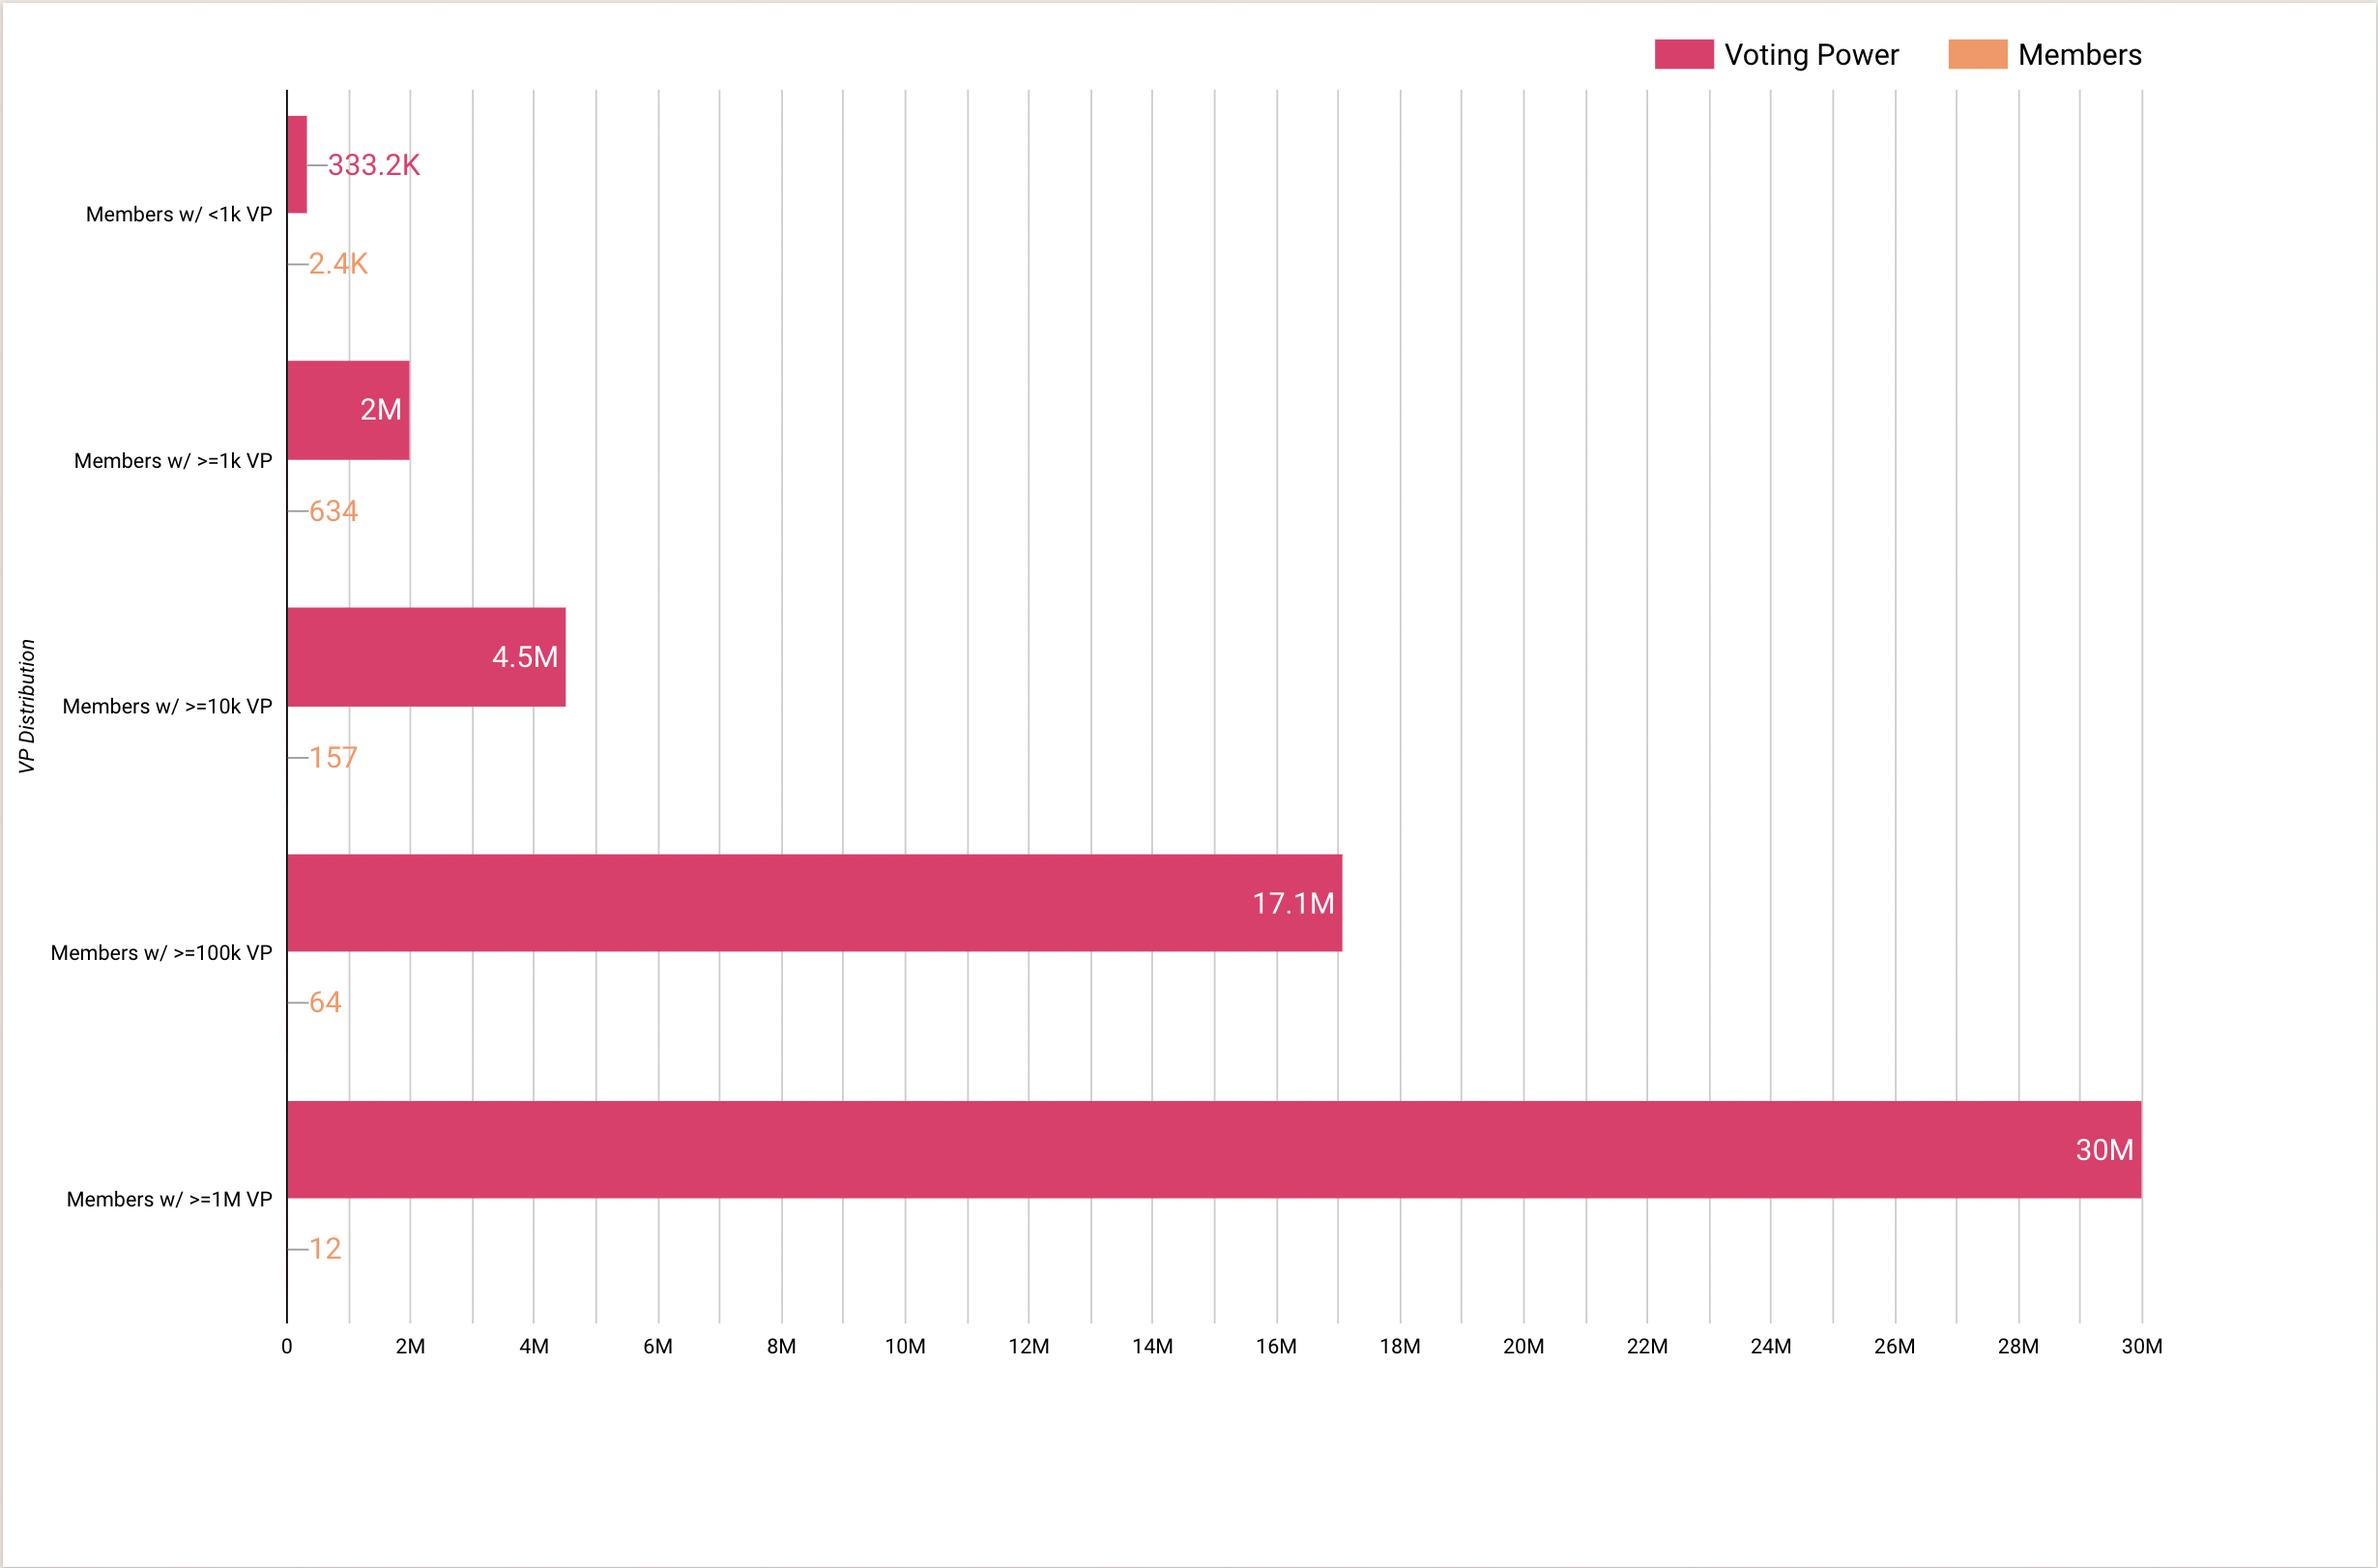
\includegraphics[width=\textwidth]{metrics/vp_distribution_members.png}
  \caption{Voting Power distribution to date}
  \label{fig:vp_distribution_members}
\end{figure}

Figure \ref{fig:vote_weight} shows by month, the average weight of votes in the final outcome of the proposals. The lower the percentage, the more distributed the voting power is. To know how the weight is calculated, see \ref{subsec_votes}.
\begin{figure}[H]
  \centering
  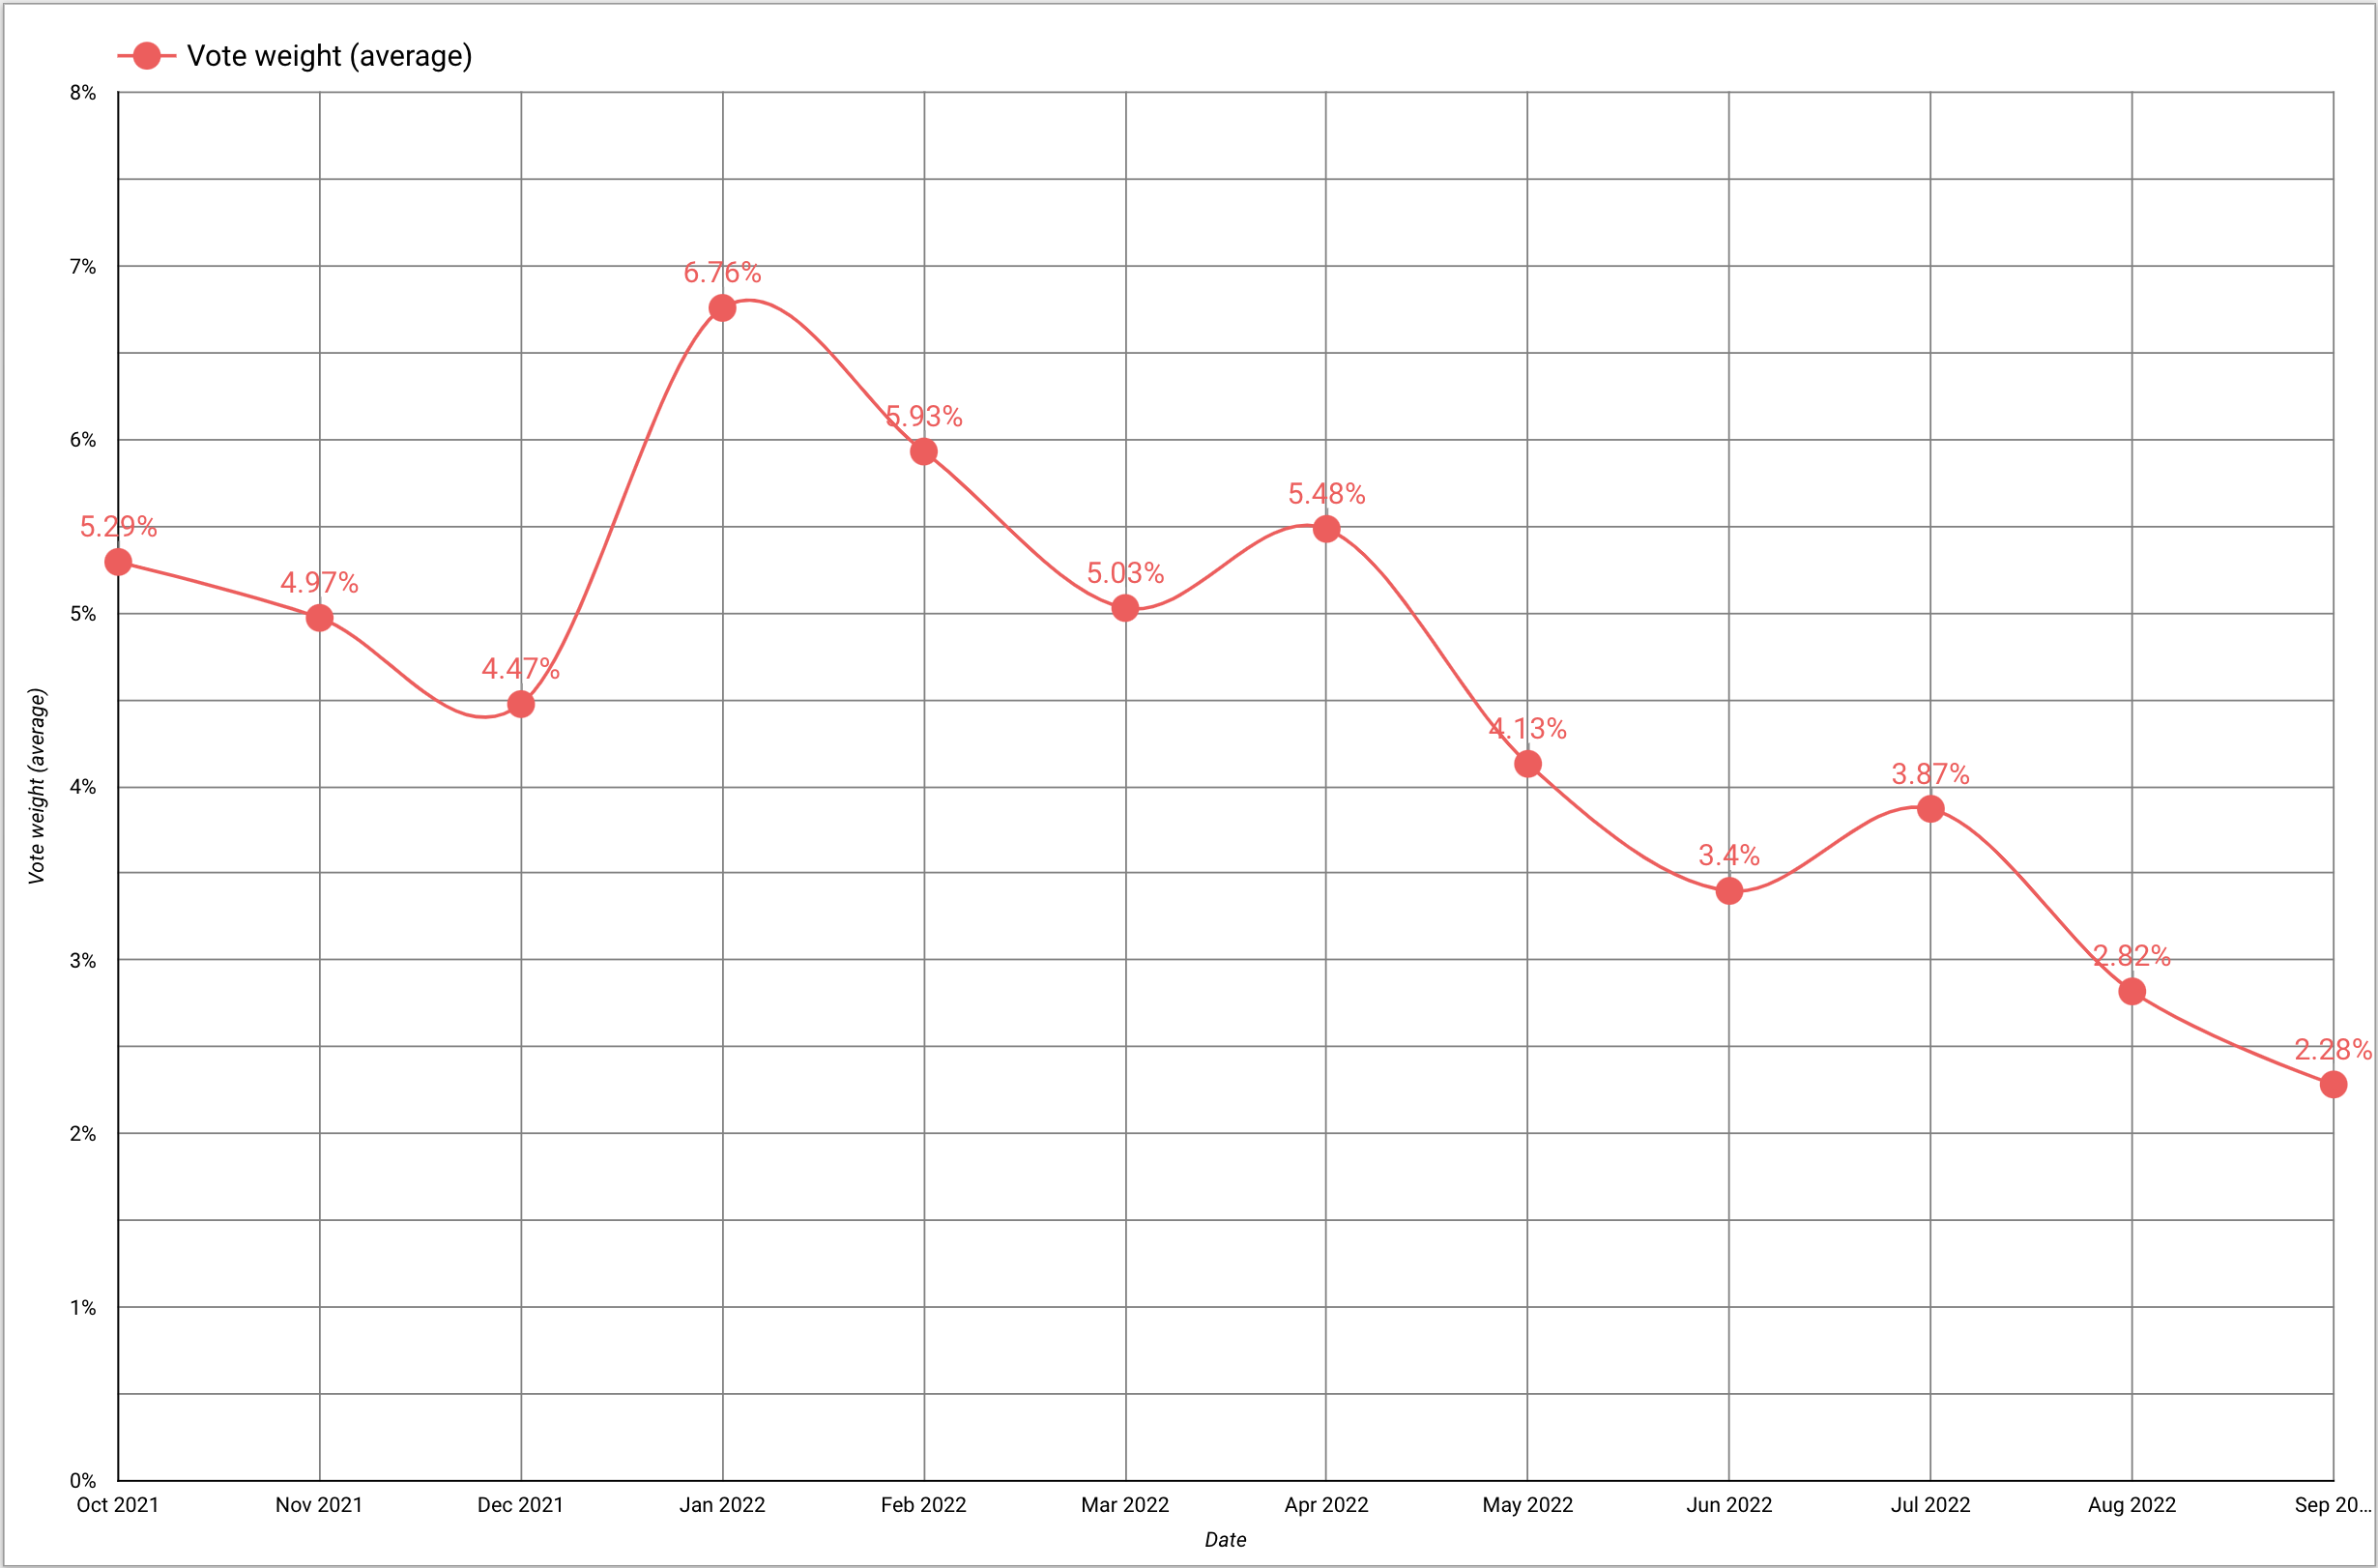
\includegraphics[width=\textwidth]{metrics/vote_weight.png}
  \caption{Average vote weight in the final outcome of the proposal}
  \label{fig:vote_weight}
\end{figure}

\section{Grants}
\begin{center}
  \begin{table}[H]
    \begin{tabular}{ | m{20em} | m{20em} | }
      \hline
      \textbf{Total enacted grants} & \textbf{Total funds granted} \\
      \hline
      100 & \$7.148.869,00 USD \\
      \hline
    \end{tabular}
    \caption{Total approved grants and funds}
    \label{table:grants}
  \end{table}
\end{center}

Figure \ref{fig:grants_amount} shows the number of grants rejected and enacted per month, with an average of 36\% of grant submissions being approved.
\begin{figure}[H]
  \centering
  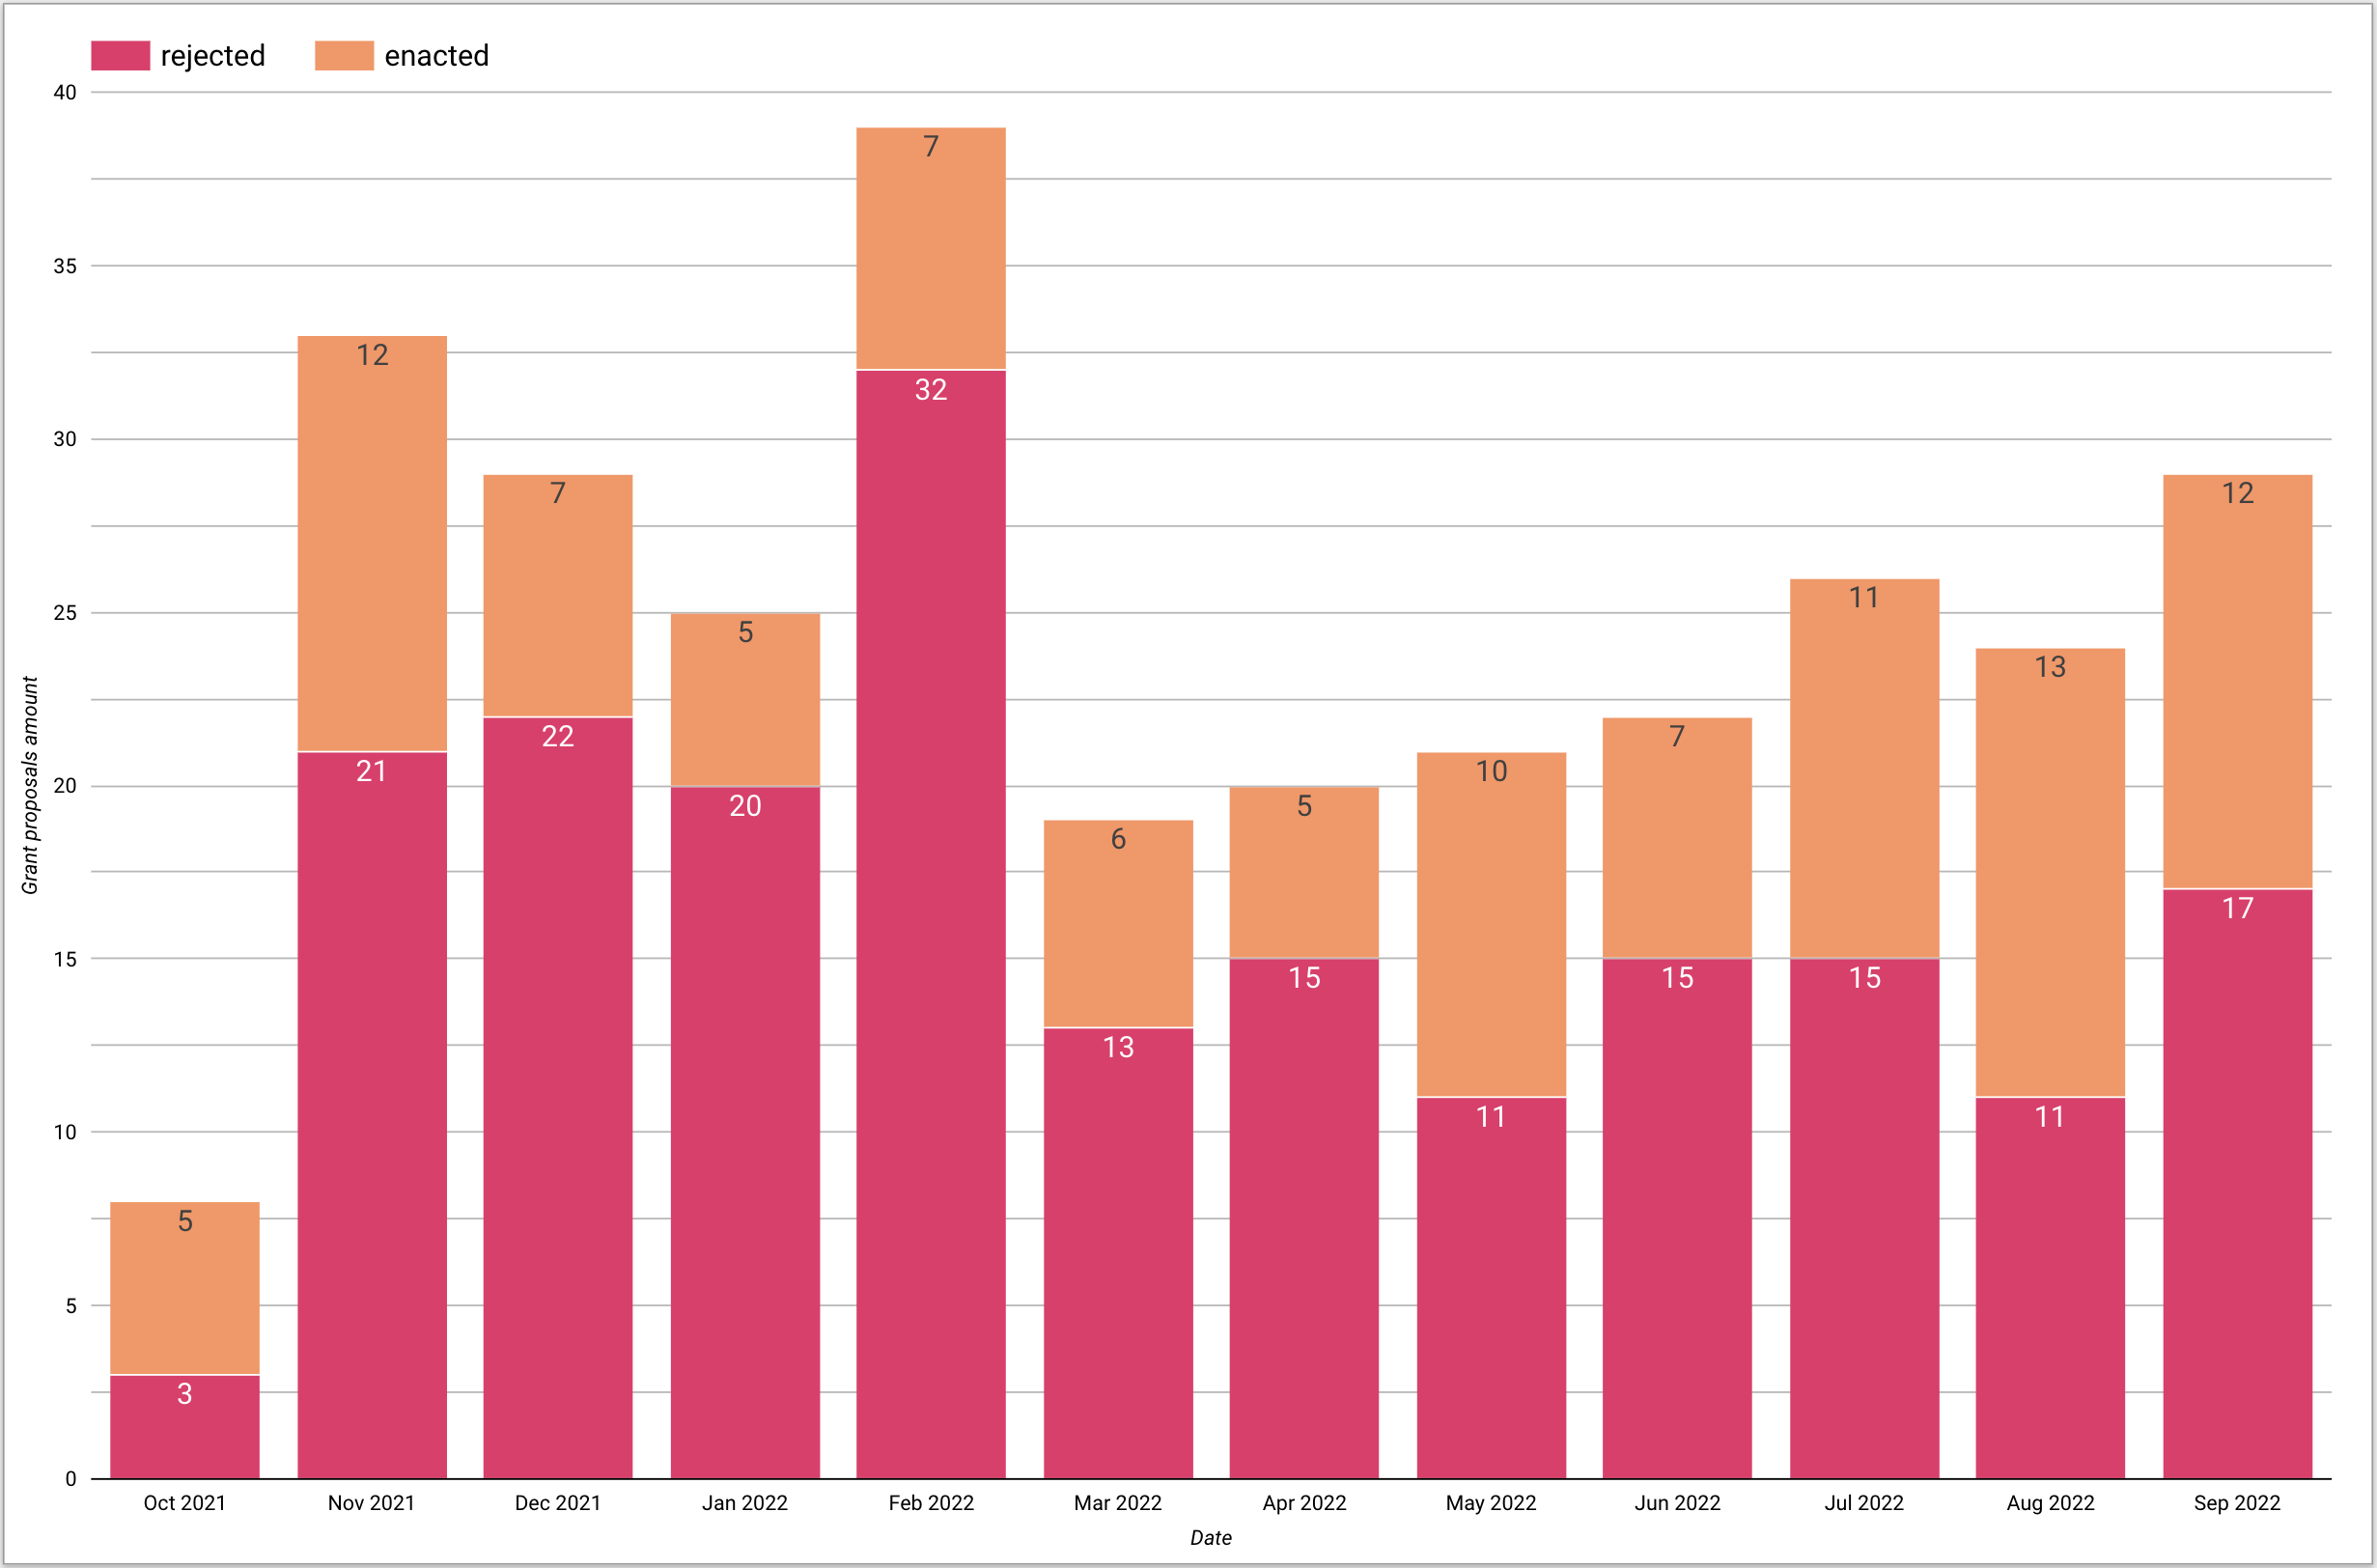
\includegraphics[width=\textwidth]{metrics/grants_amount.png}
  \caption{Enacted and rejected grants amount per month}
  \label{fig:grants_amount}
\end{figure}

Figure \ref{fig:funds_granted} shows the amount of funds allocated to grants per month. If the number o grants enacted per month from Figure \ref{fig:grants_amount} is considered, it gives a median of US\$79,400 per grant.
\begin{figure}[H]
  \centering
  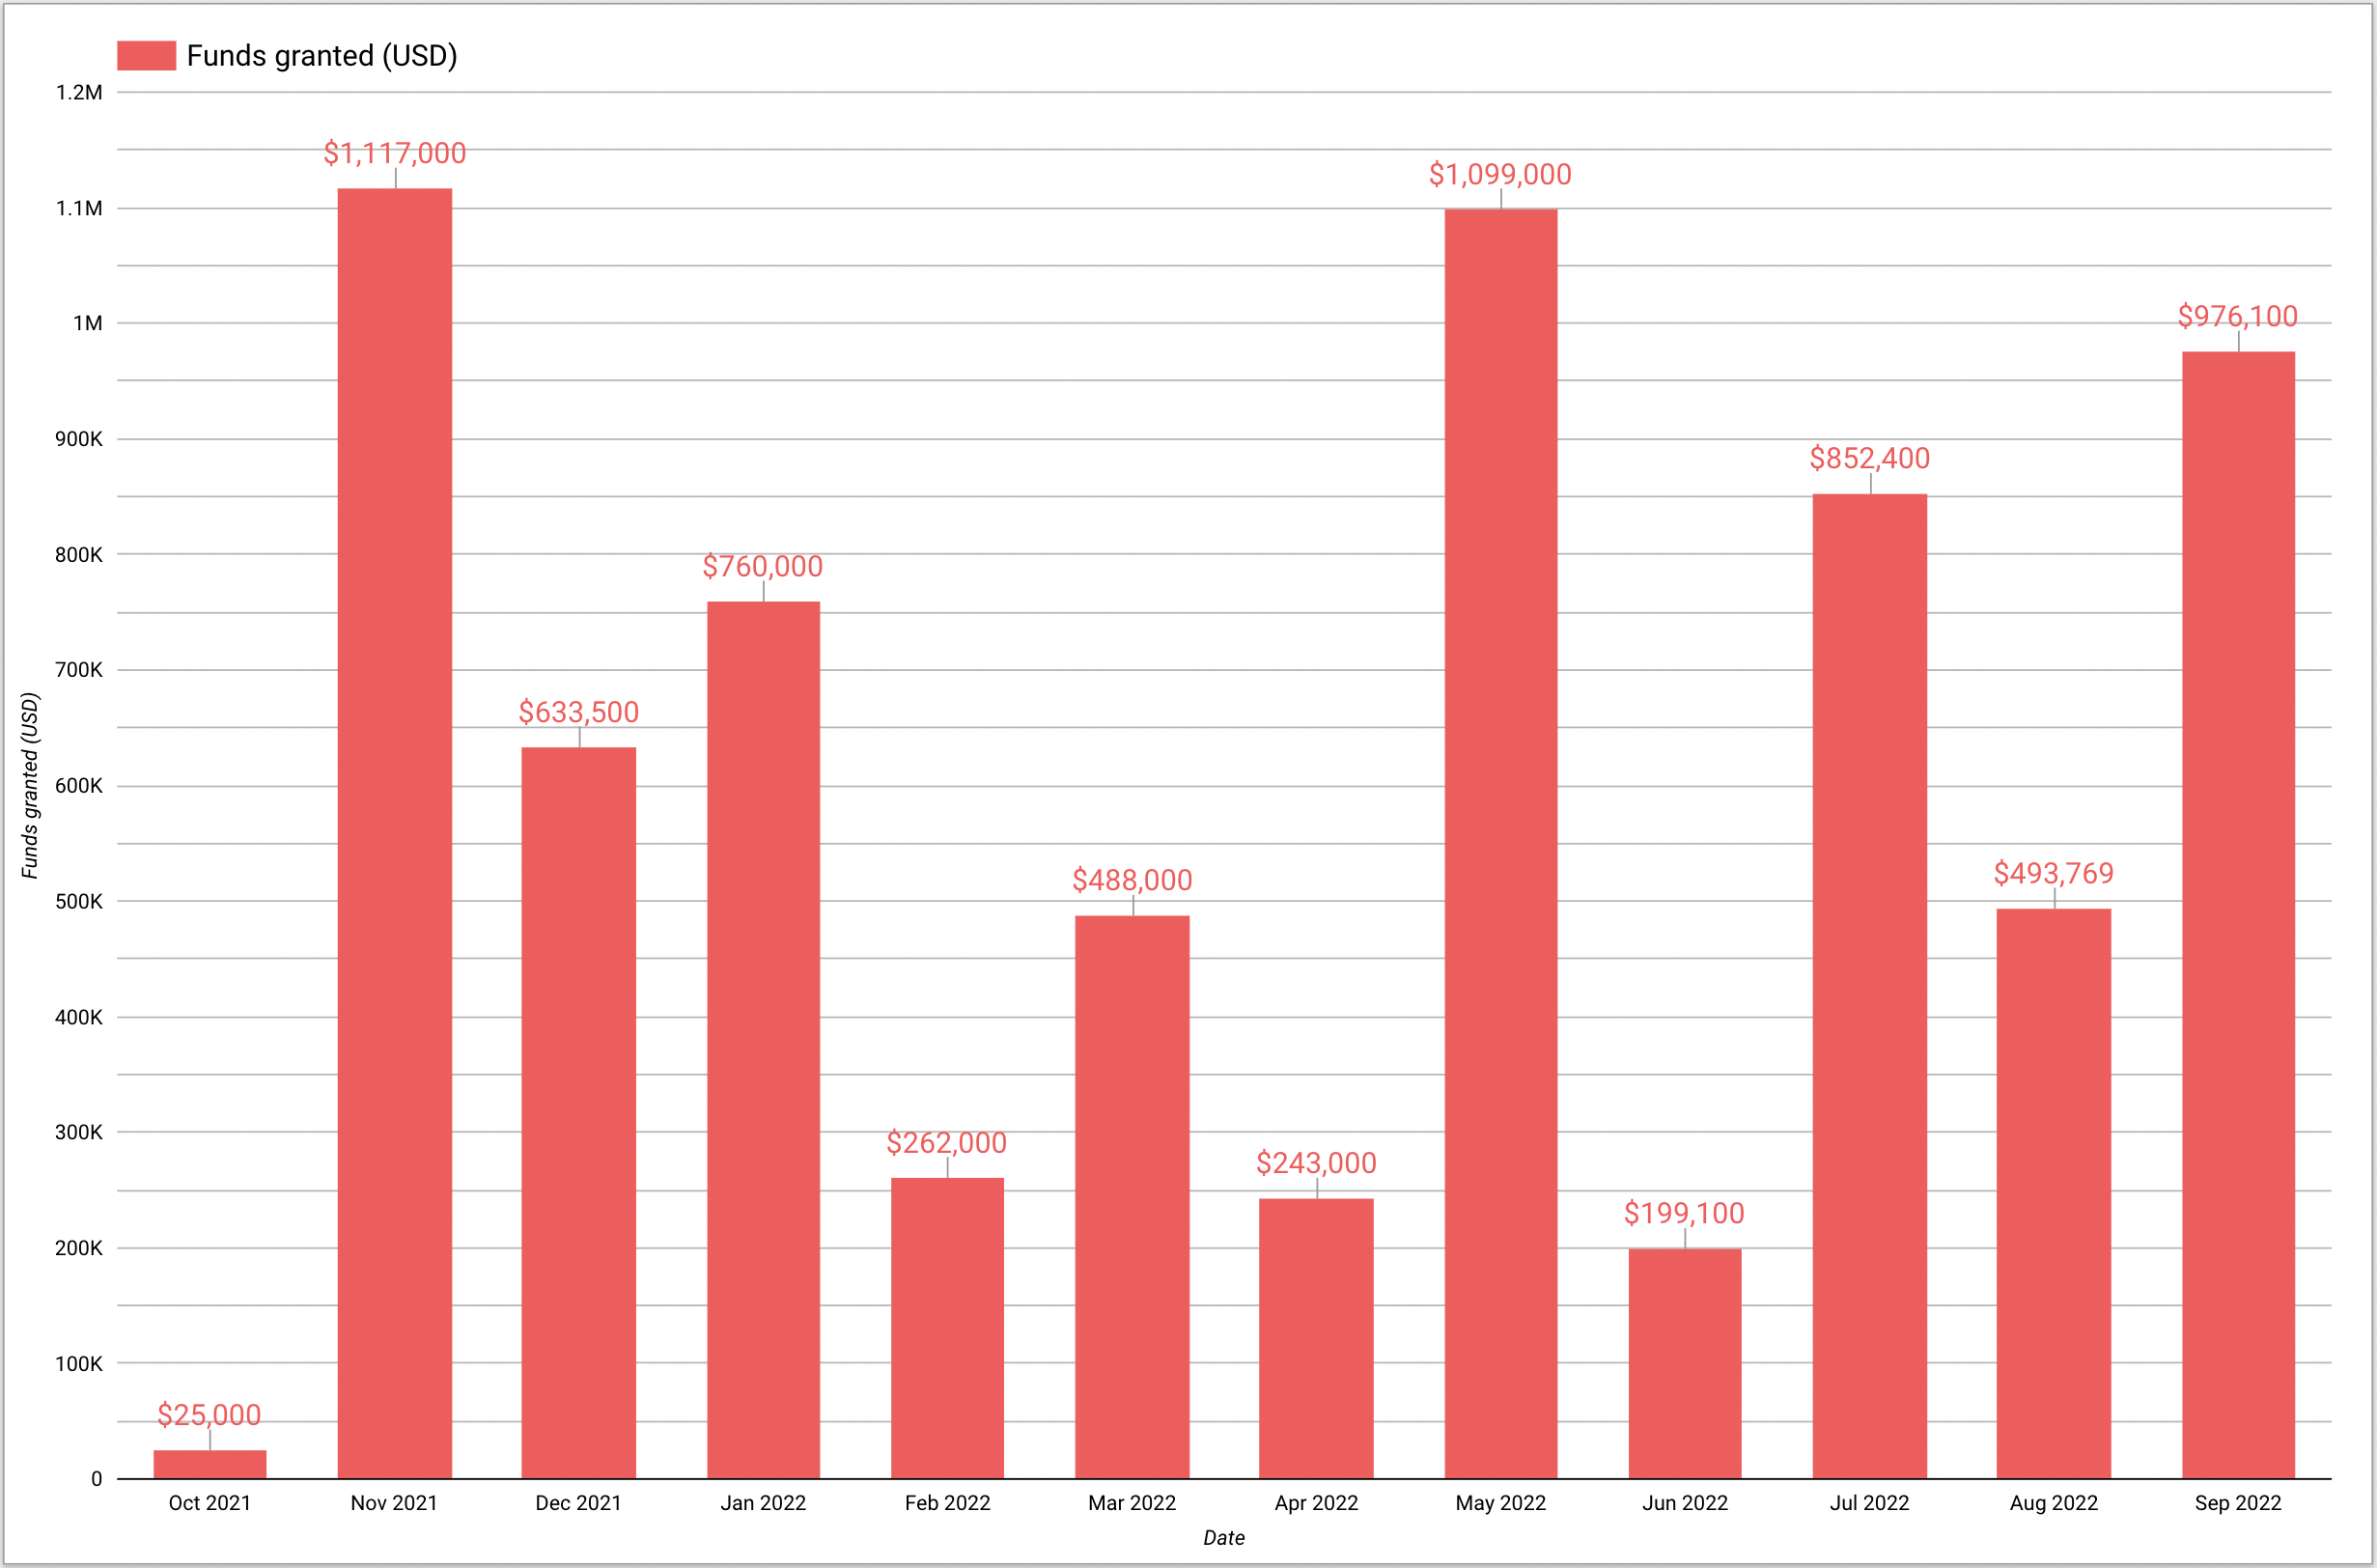
\includegraphics[width=\textwidth]{metrics/funds_granted.png}
  \caption{Funds granted per month}
  \label{fig:funds_granted}
\end{figure}

Figure \ref{fig:funds_recovered} shows the amount of funds that returned to the DAO from unfinished grants.
\begin{figure}[H]
  \centering
  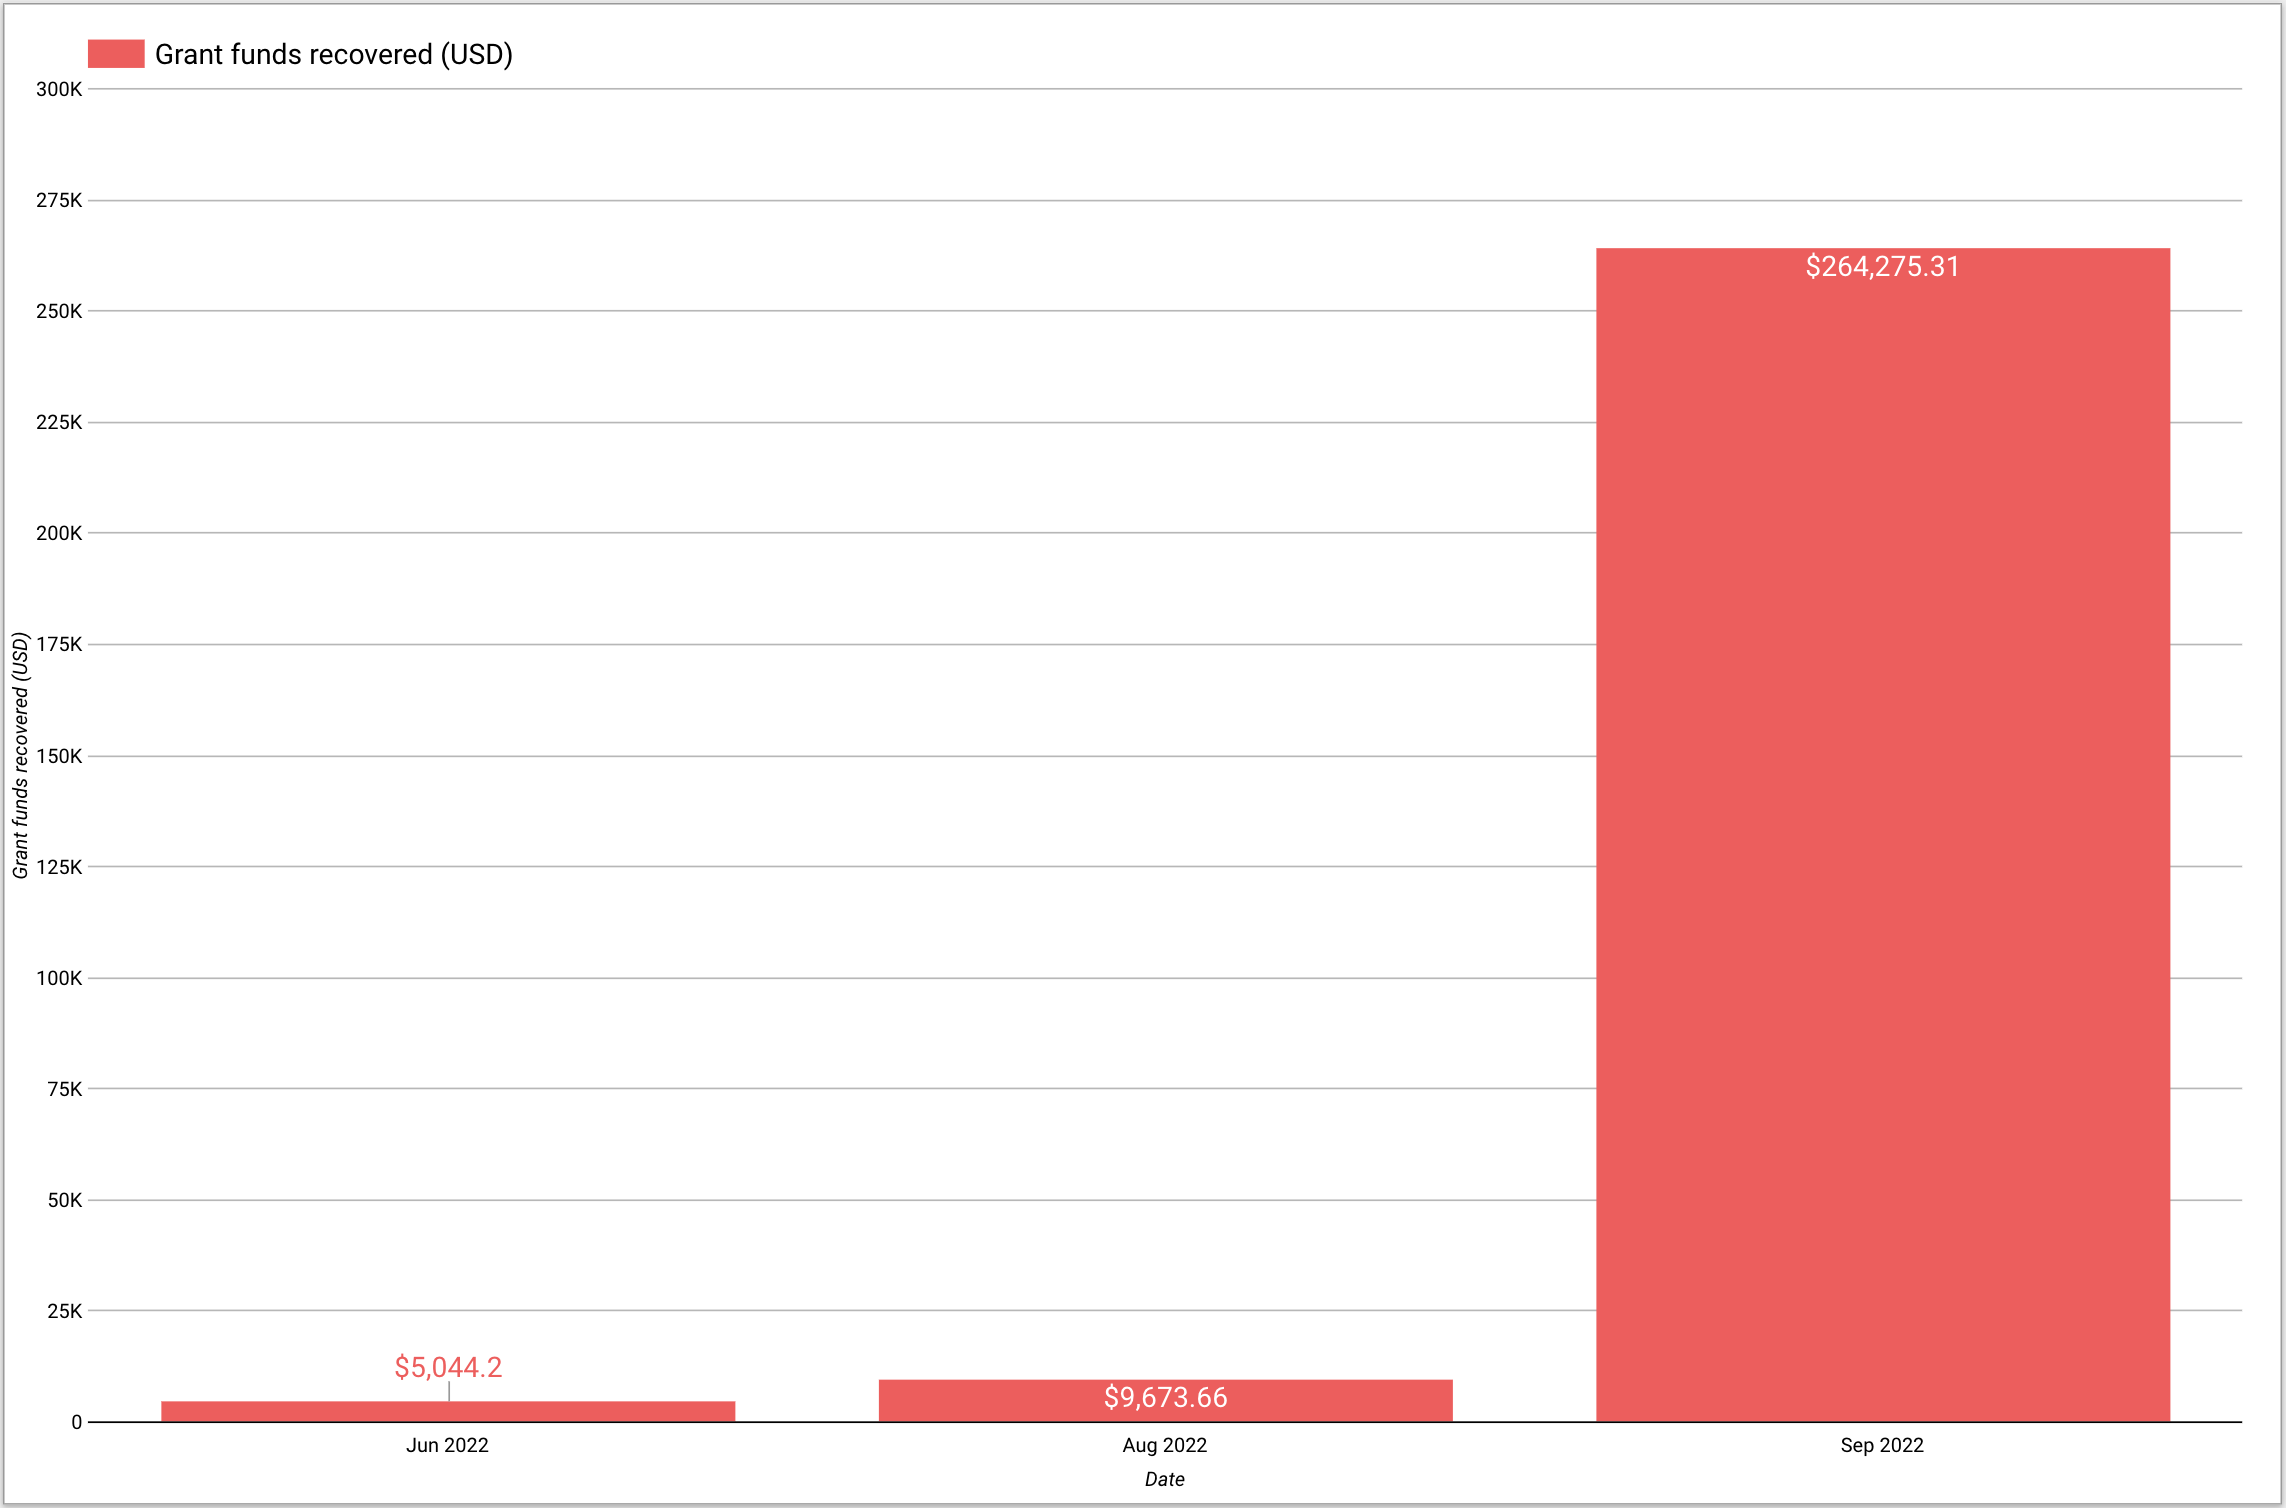
\includegraphics[width=\textwidth]{metrics/funds_recovered.png}
  \caption{Grant funds recovered per month}
  \label{fig:funds_recovered}
\end{figure}

Figure \ref{fig:category_distribution} shows how the categories of grants enacted are distributed, indicating that they are evenly distributed.
\begin{figure}[H]
  \centering
  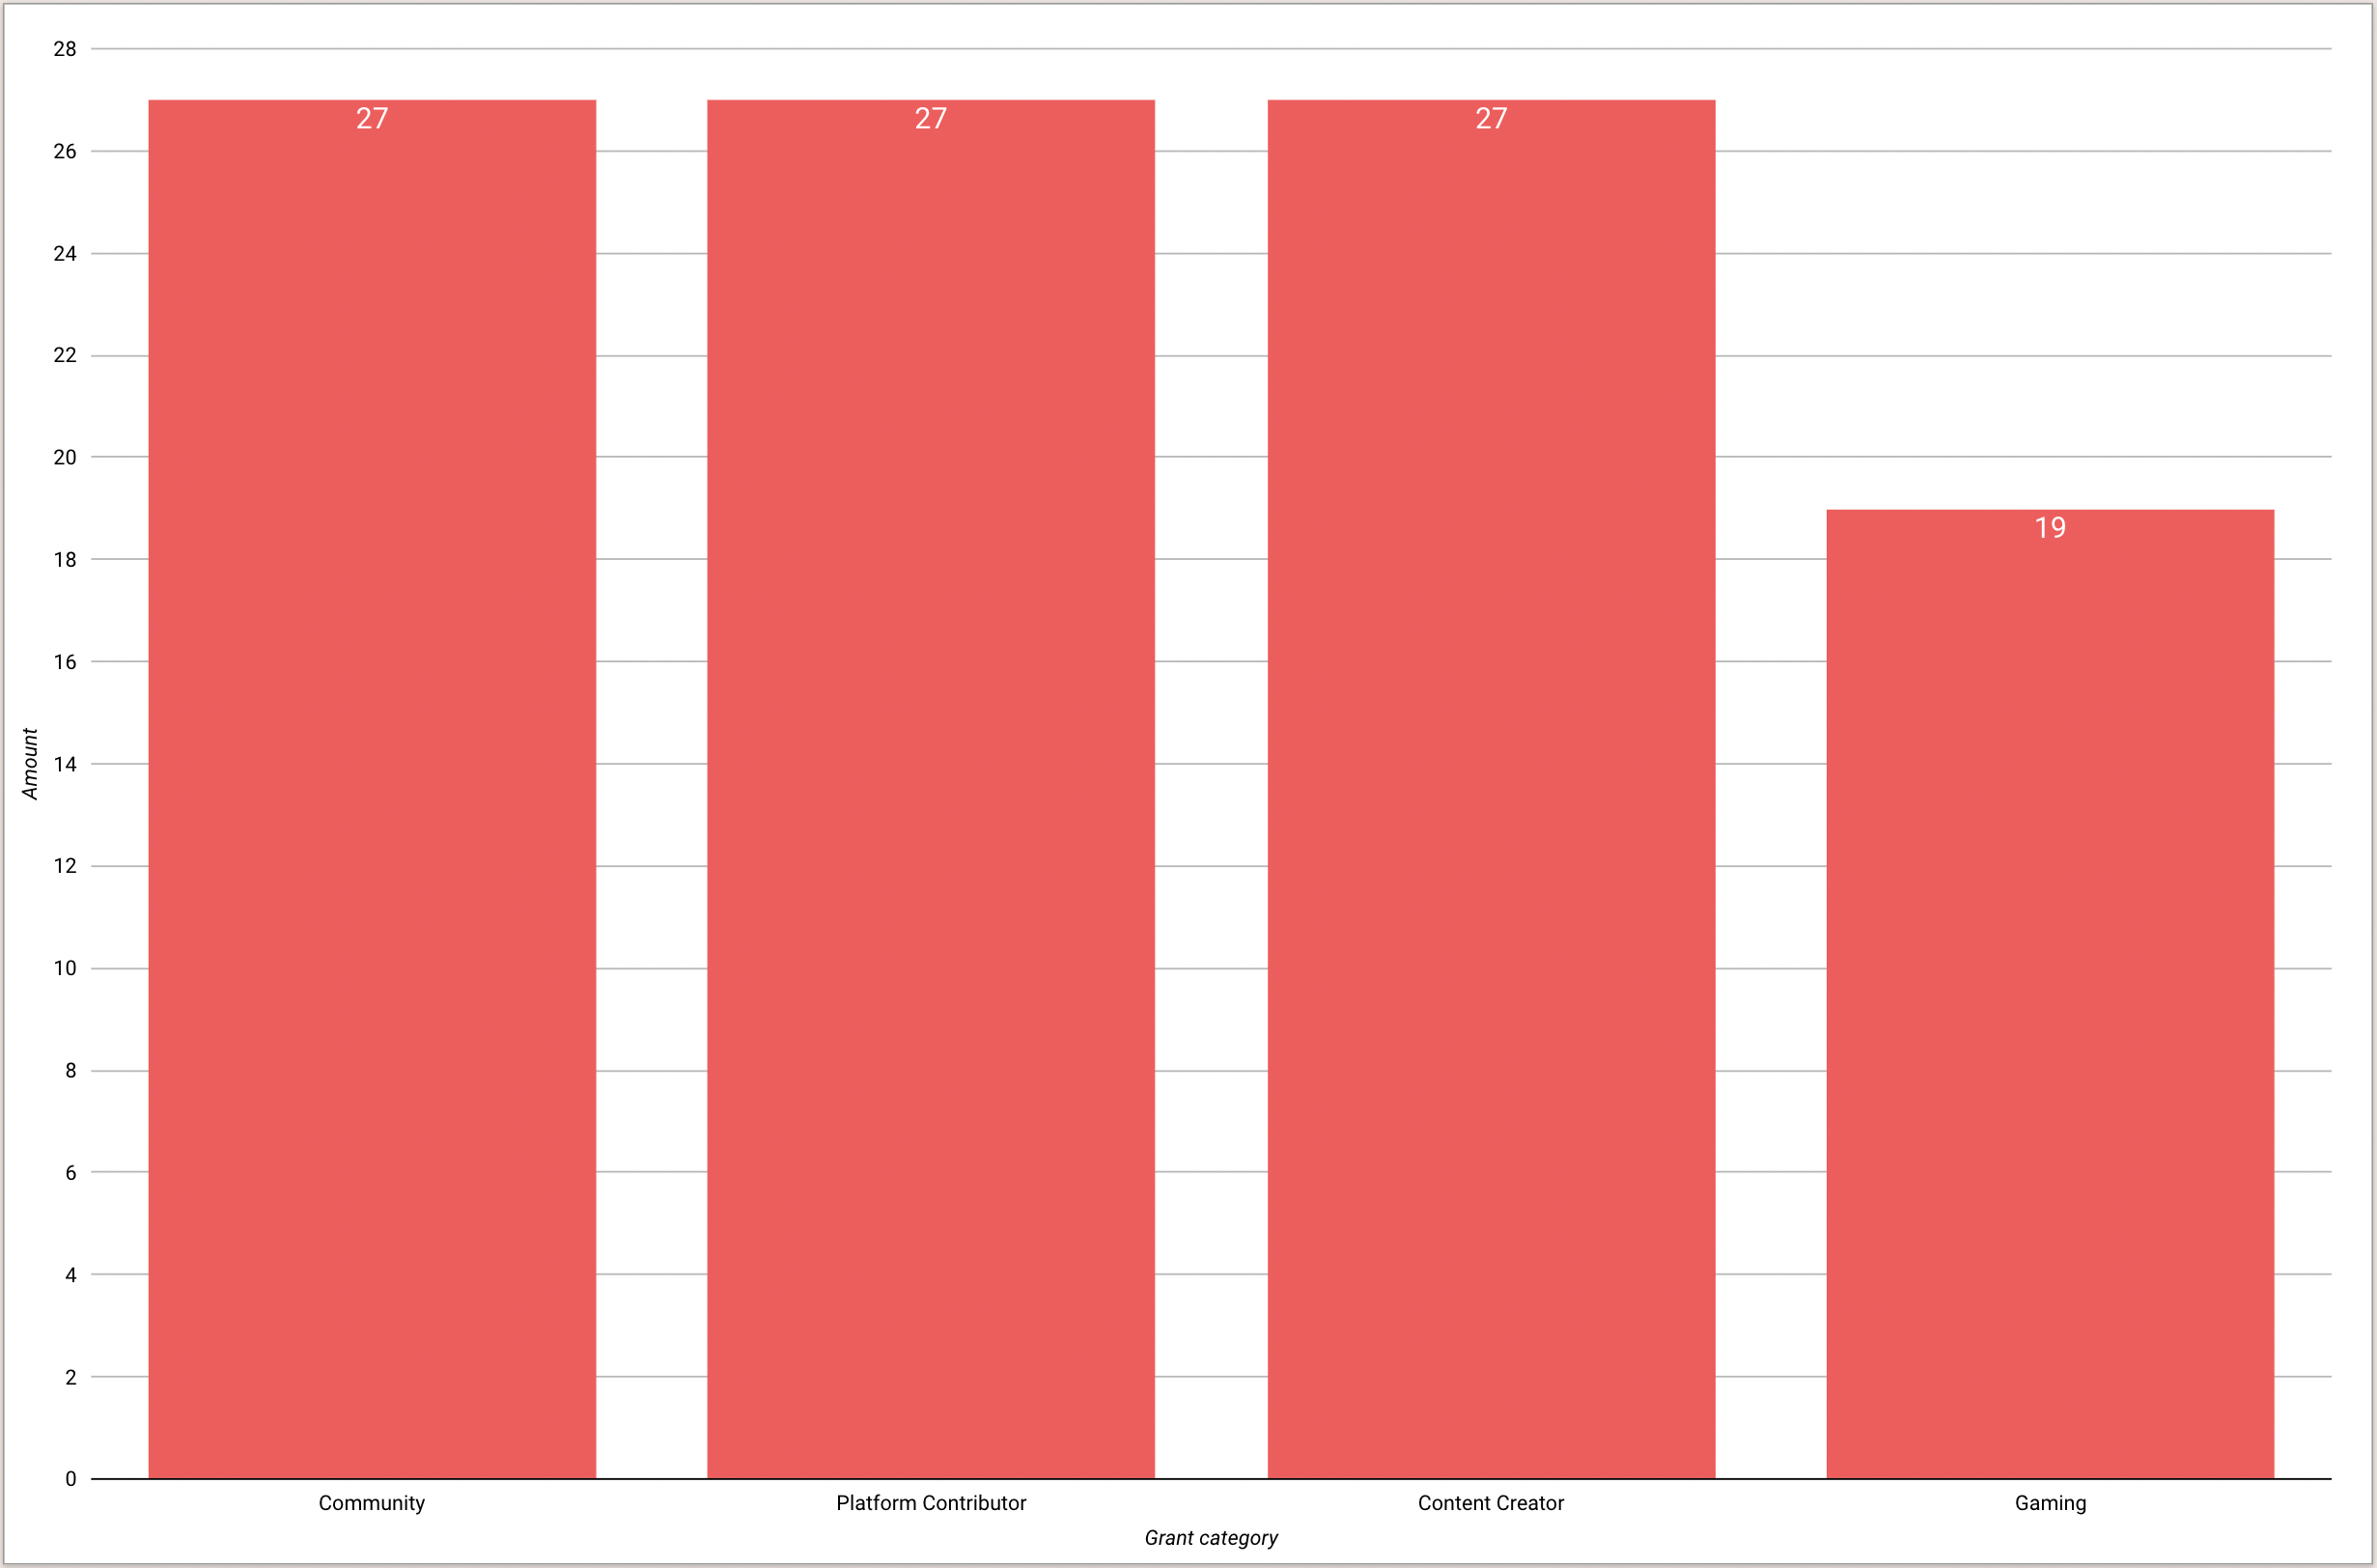
\includegraphics[width=\textwidth]{metrics/category_distribution.png}
  \caption{Enacted grants category distribution (*)}
  \label{fig:category_distribution}
\end{figure}

(*) Detail of grant categories\cite{grants}:
\begin{itemize}
  \item \textbf{Community}: Grants under this category may fund activity such as community education, outreach and event organization or moderation. Projects might also include creating documentation, tutorials, videos, or other forms of content intended to educate and support the community.
  \item \textbf{Content Creator}: Grants in this category help to support artists to create scenes and models for Decentraland.
  \item \textbf{Platform Contributor}: Grants within the Builder category should motivate and reward impactful contributions from developers and engineers in the form of new features, bug fixes, and other improvements to existing code.
  \item \textbf{Gaming}: This category bridges the Creator and Platform Contributor categories by funding individuals and teams committed to building complete games for Decentraland.
\end{itemize}

Figure \ref{fig:tier_distribution} shows the distribution of grant tiers requested, with Tier 4 (between US\$5,000 and US\$60,000) being the most requested.
\begin{figure}[H]
  \centering
  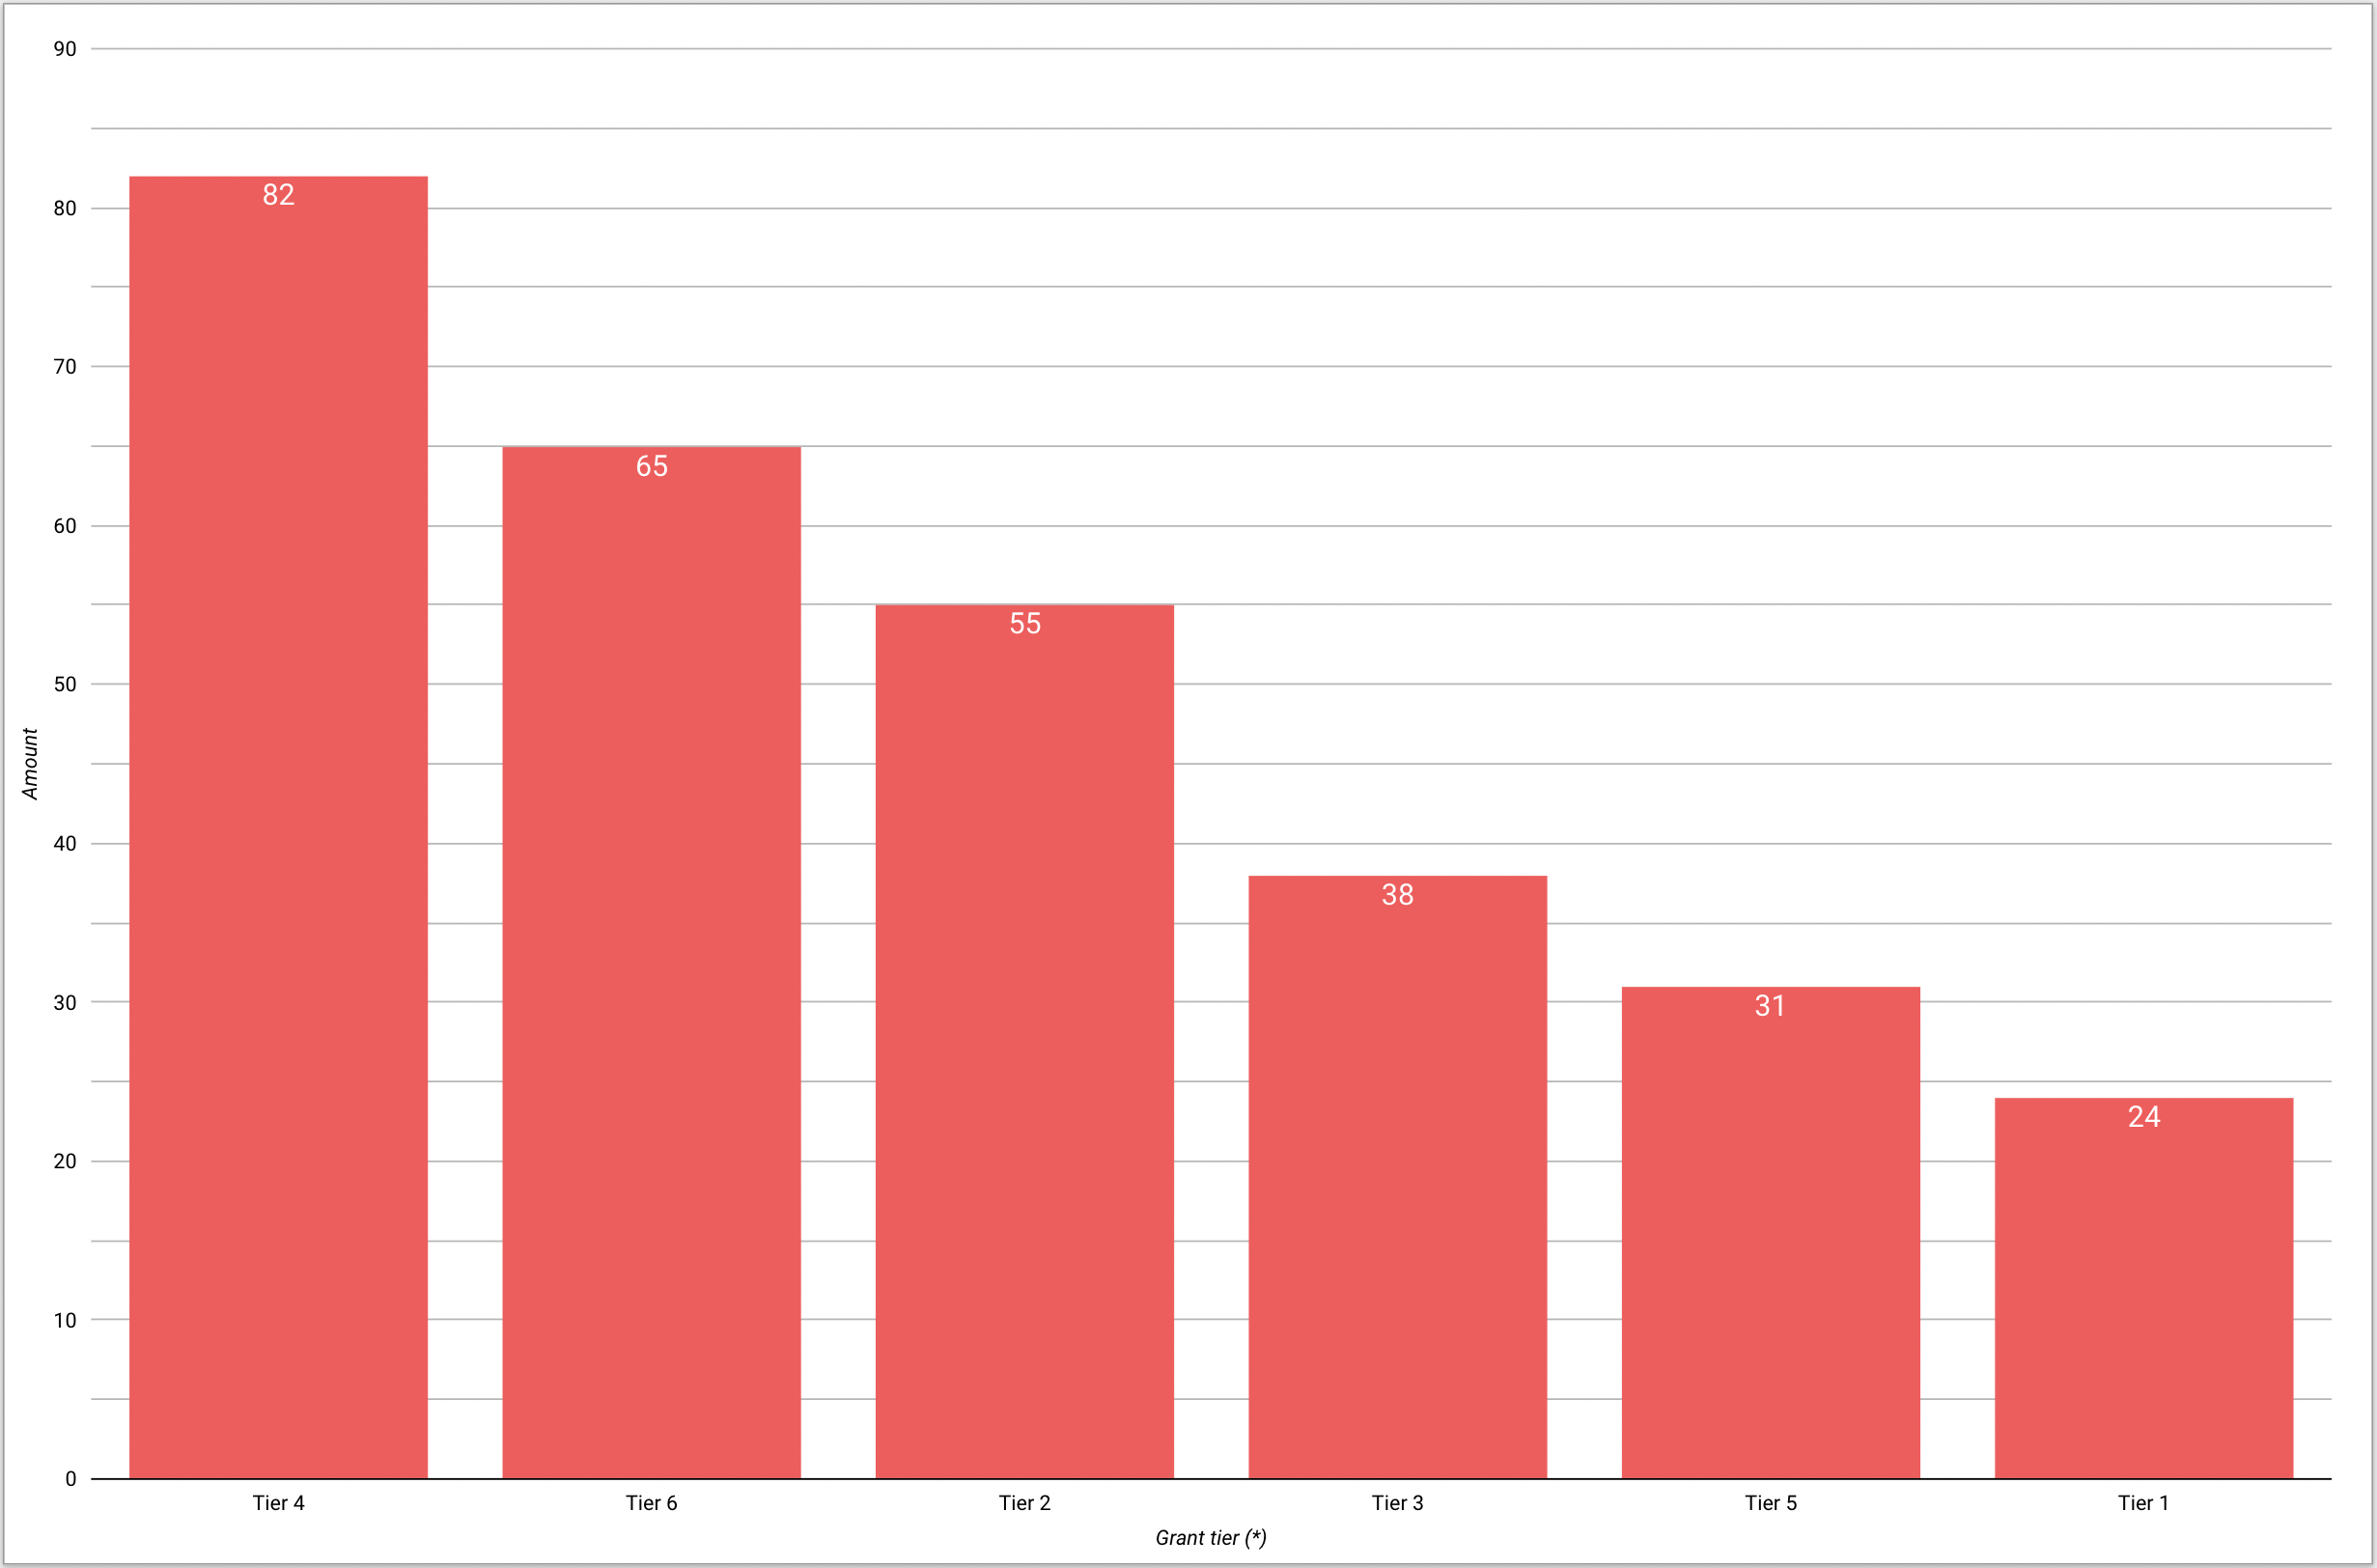
\includegraphics[width=\textwidth]{metrics/tier_distribution.png}
  \caption{Grant tiers distribution}
  \label{fig:tier_distribution}
\end{figure}
(*) Tier 1: up to \$1.500 USD - Tier 2: up to \$3.000 USD - Tier 3: up to \$5.000 USD - Tier 4: up to \$60.000 USD - Tier 5: up to \$120.000 USD - Tier 6: up to \$240.000 USD

\section{DAO Balances}

Figure \ref{fig:dao_balance} and \ref{fig:token_distribution} shows how the tokens in the different DAO wallets are allocated, with MANA being the main one as of the date of this writing. Said token represents 99\% of the holdings.
\begin{figure}[H]
  \centering
  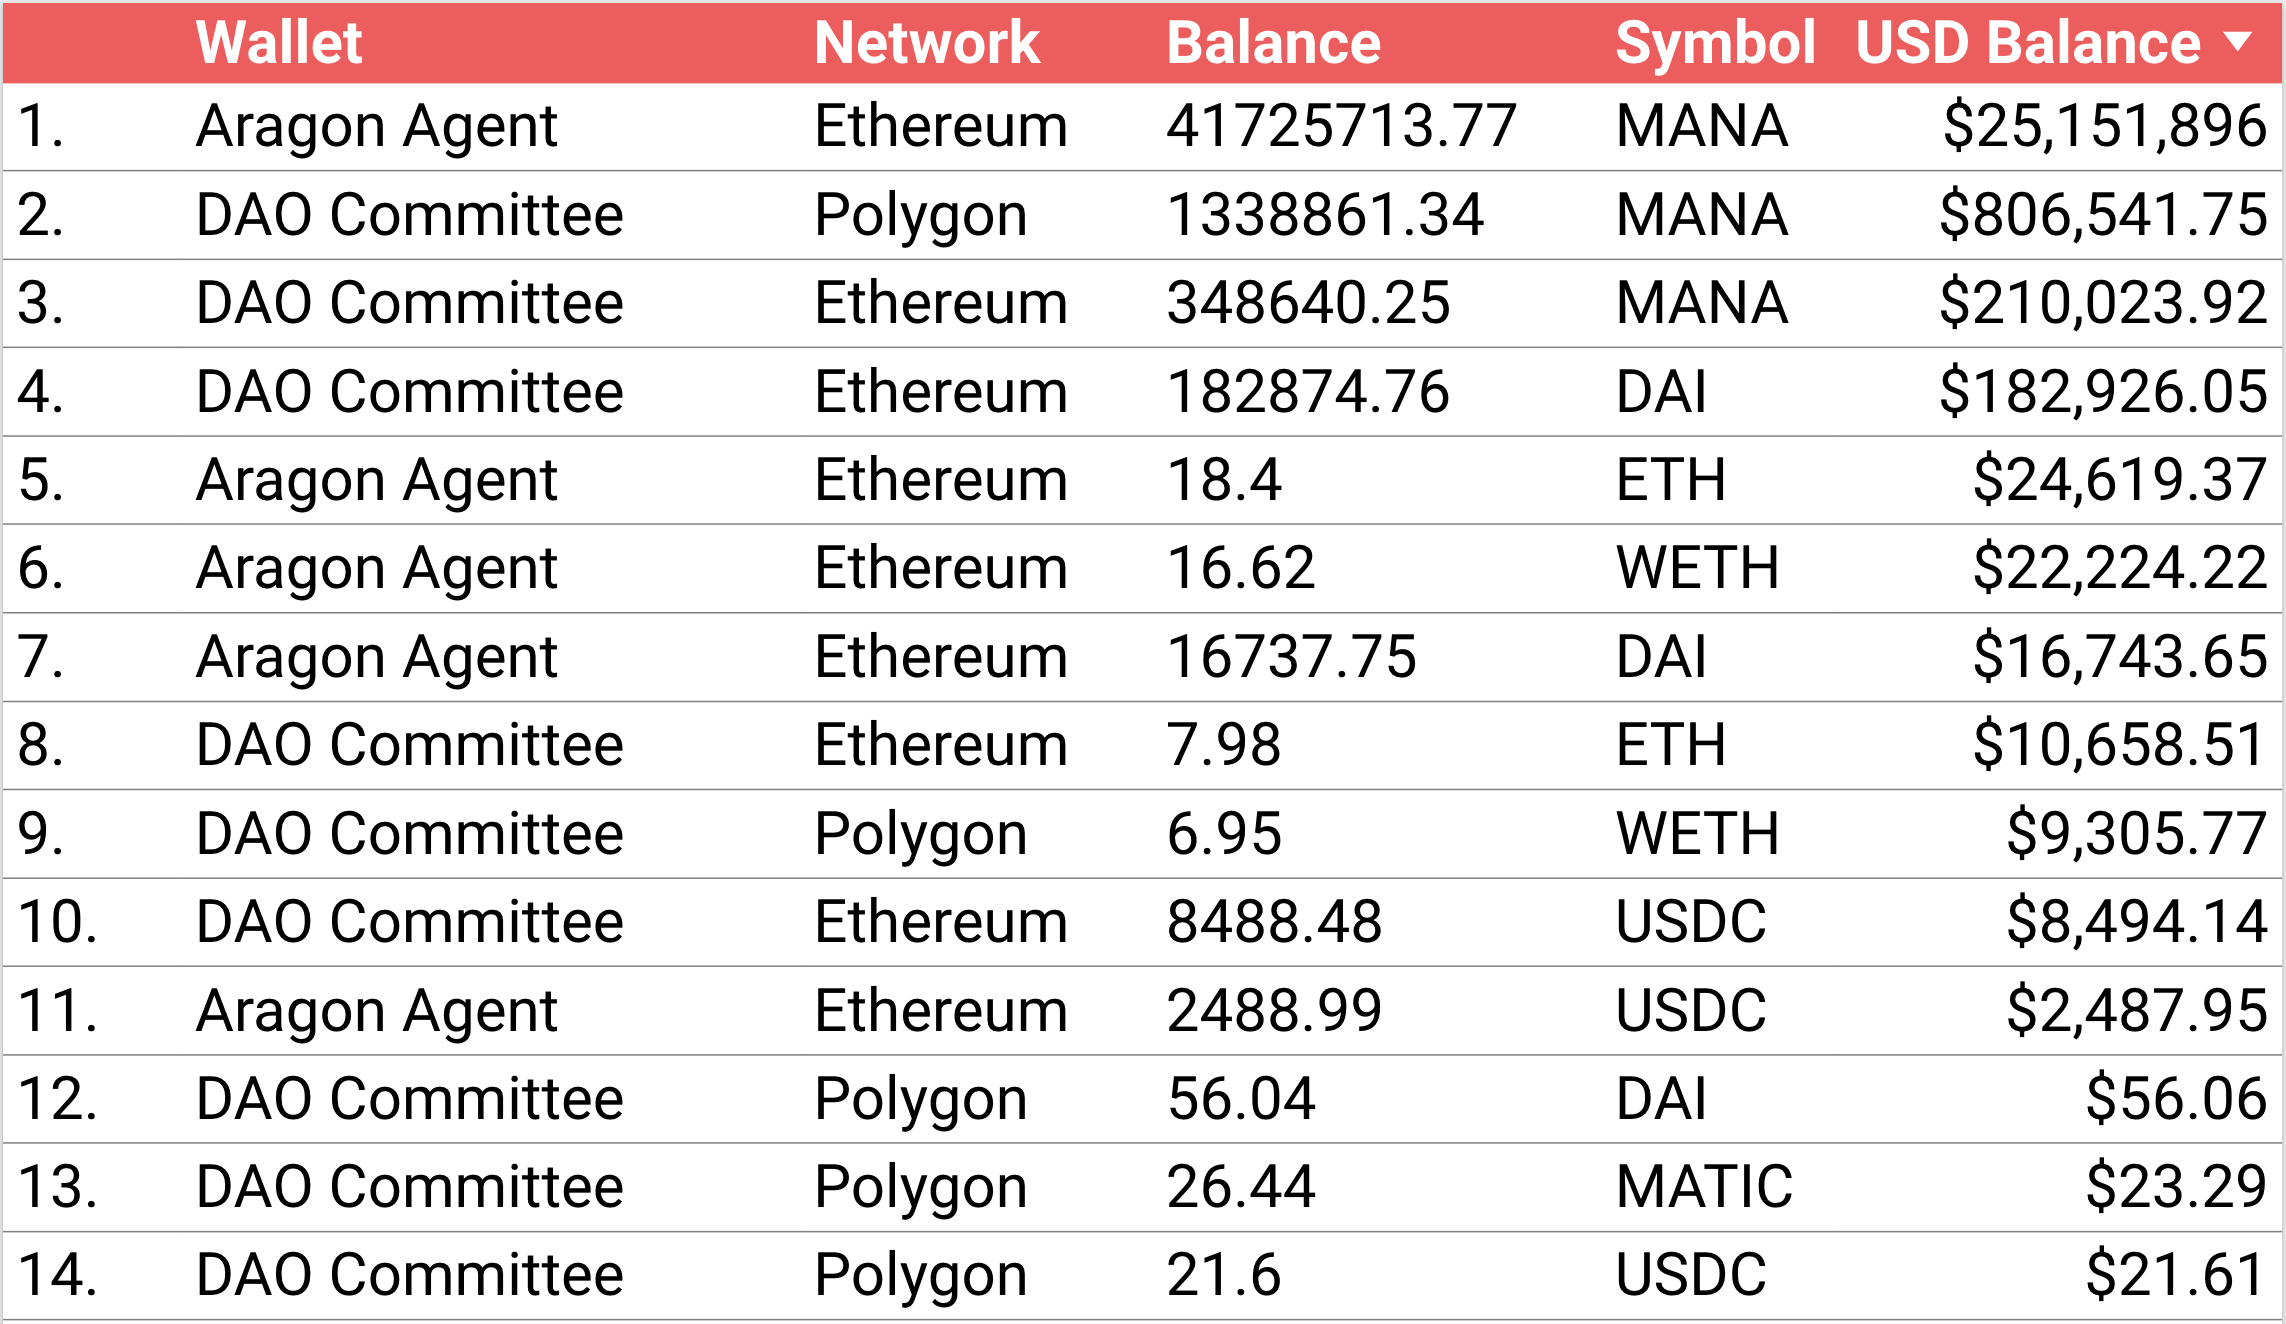
\includegraphics[width=\textwidth]{metrics/dao_balance.png}
  \caption{DAO wallets balance to date}
  \label{fig:dao_balance}
\end{figure}
\begin{figure}[H]
  \centering
  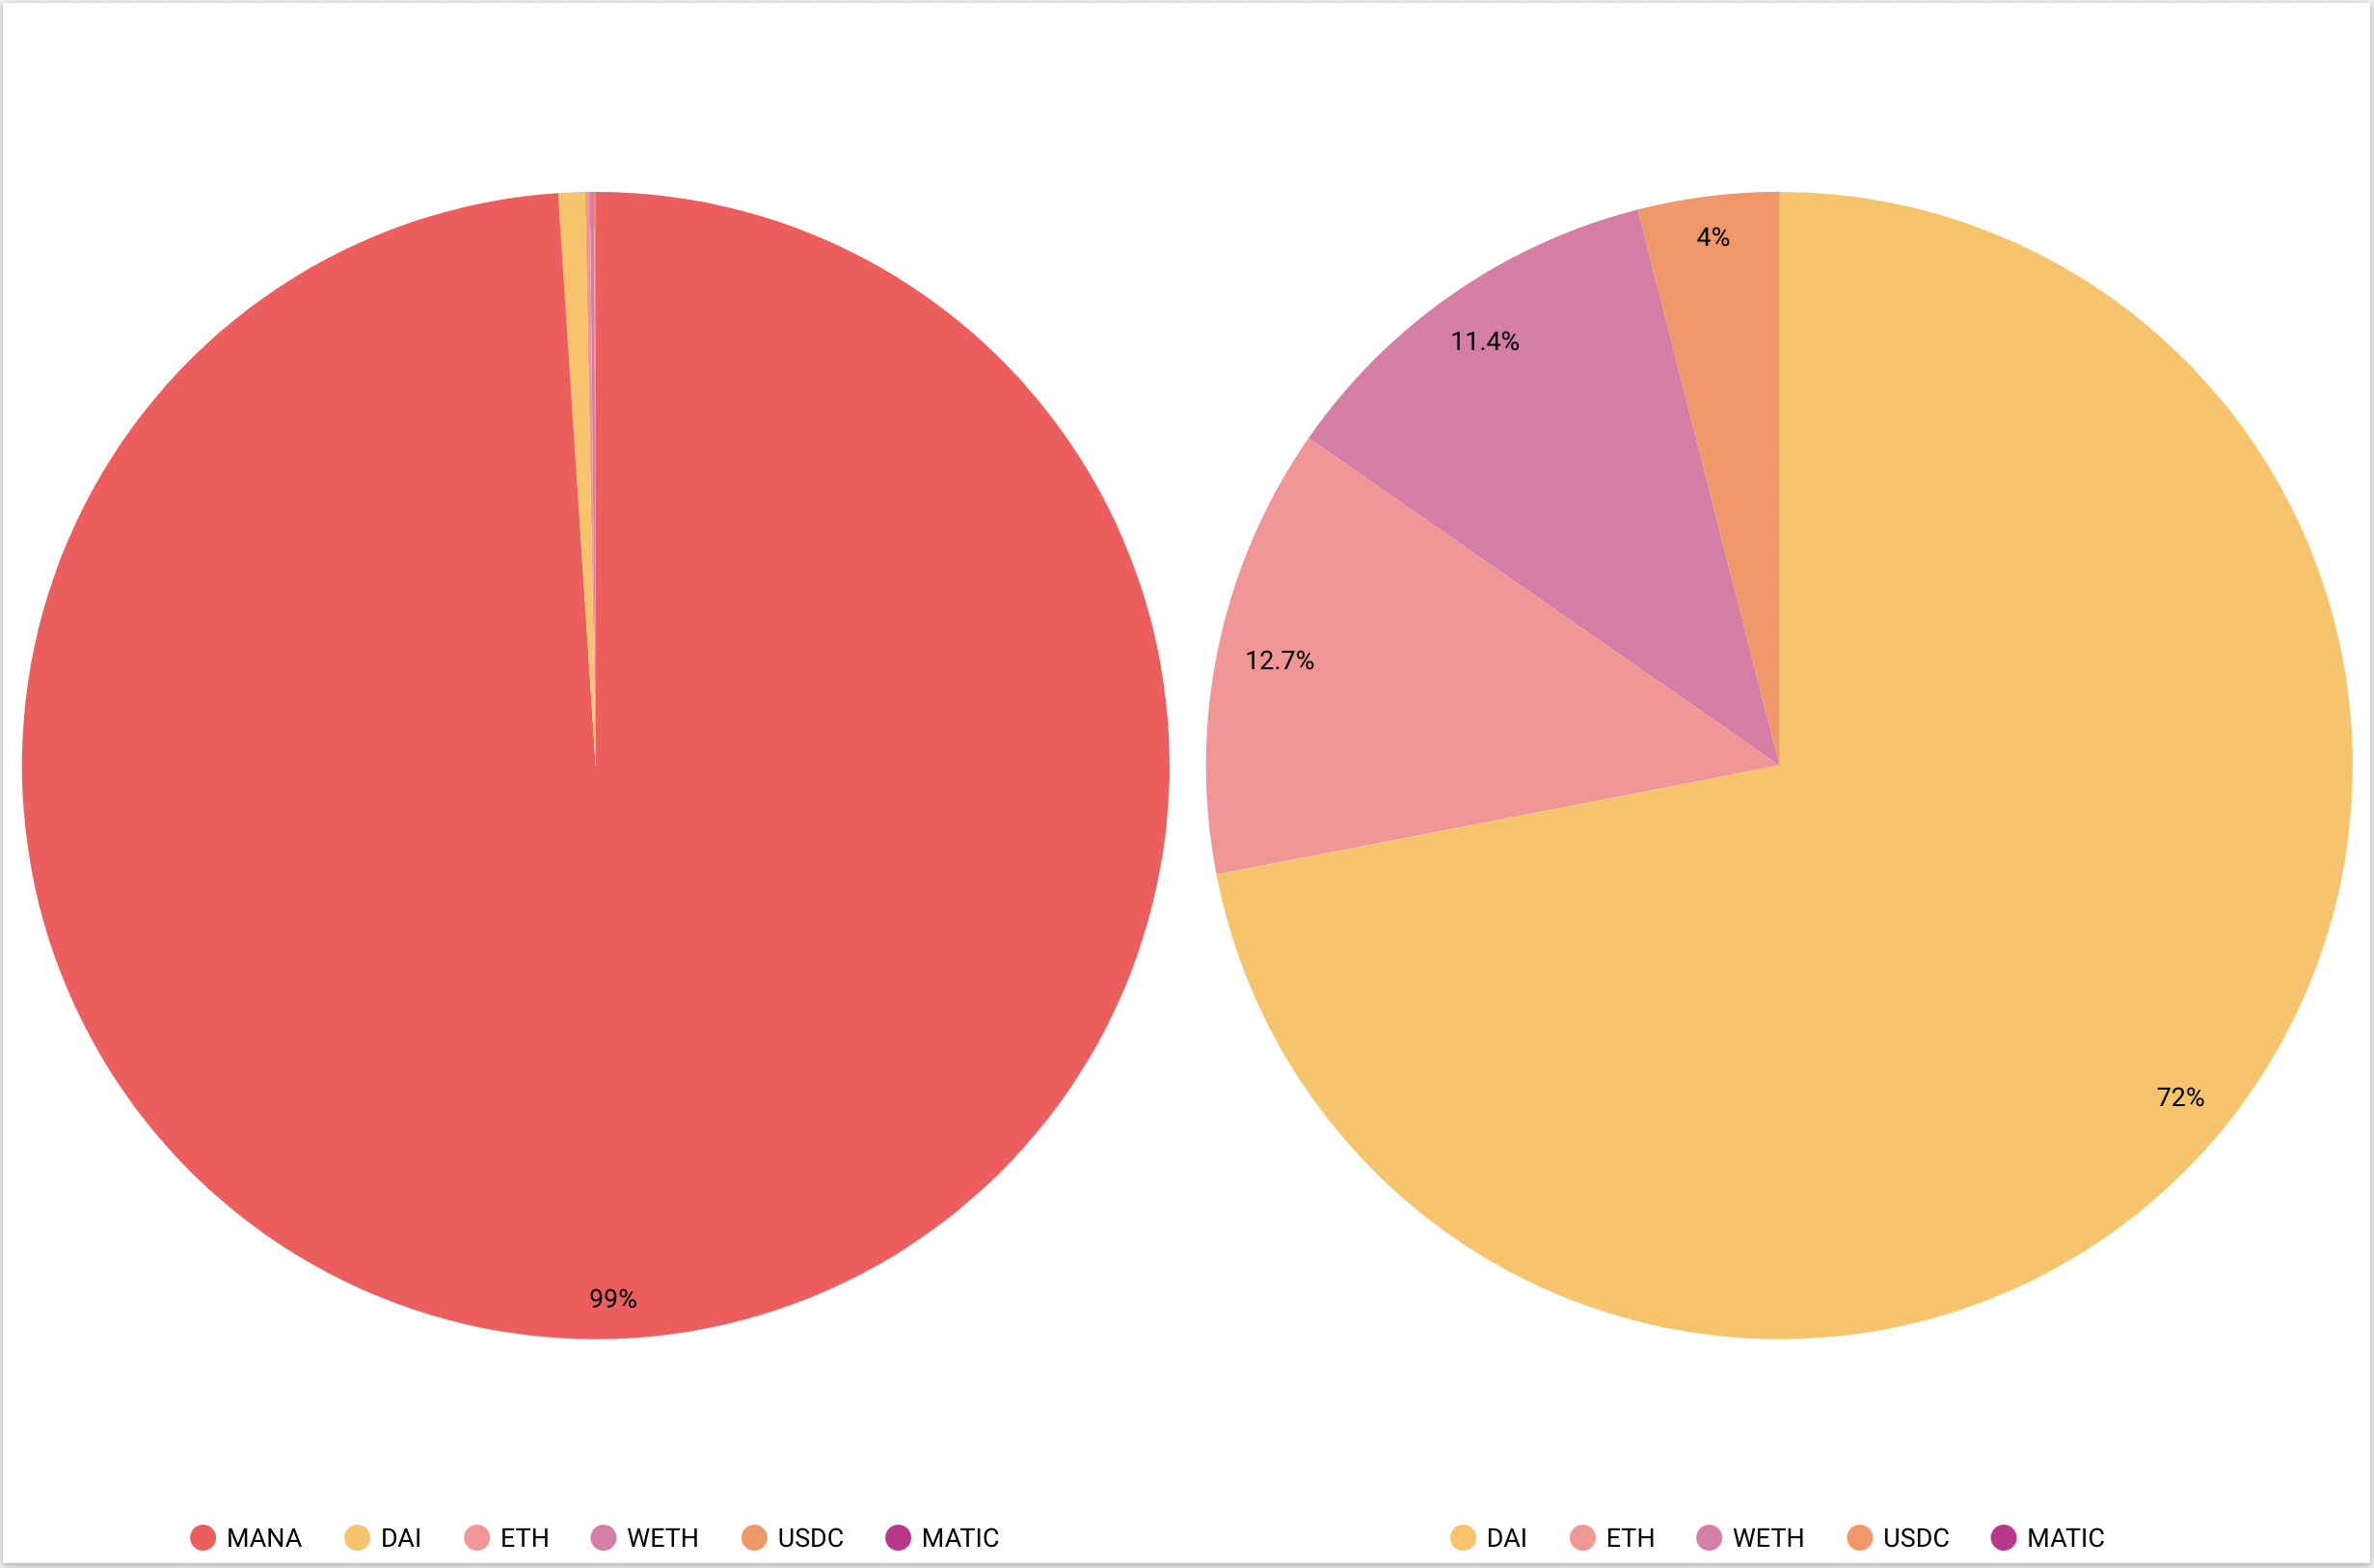
\includegraphics[width=\textwidth]{metrics/token_distribution.png}
  \caption{Distribution of tokens in DAO wallets to date}
  \label{fig:token_distribution}
\end{figure}

Figure \ref{fig:income} shows the DAO revenue sources by month and by category, highlighting cells based on their values.
\begin{figure}[H]
  \centering
  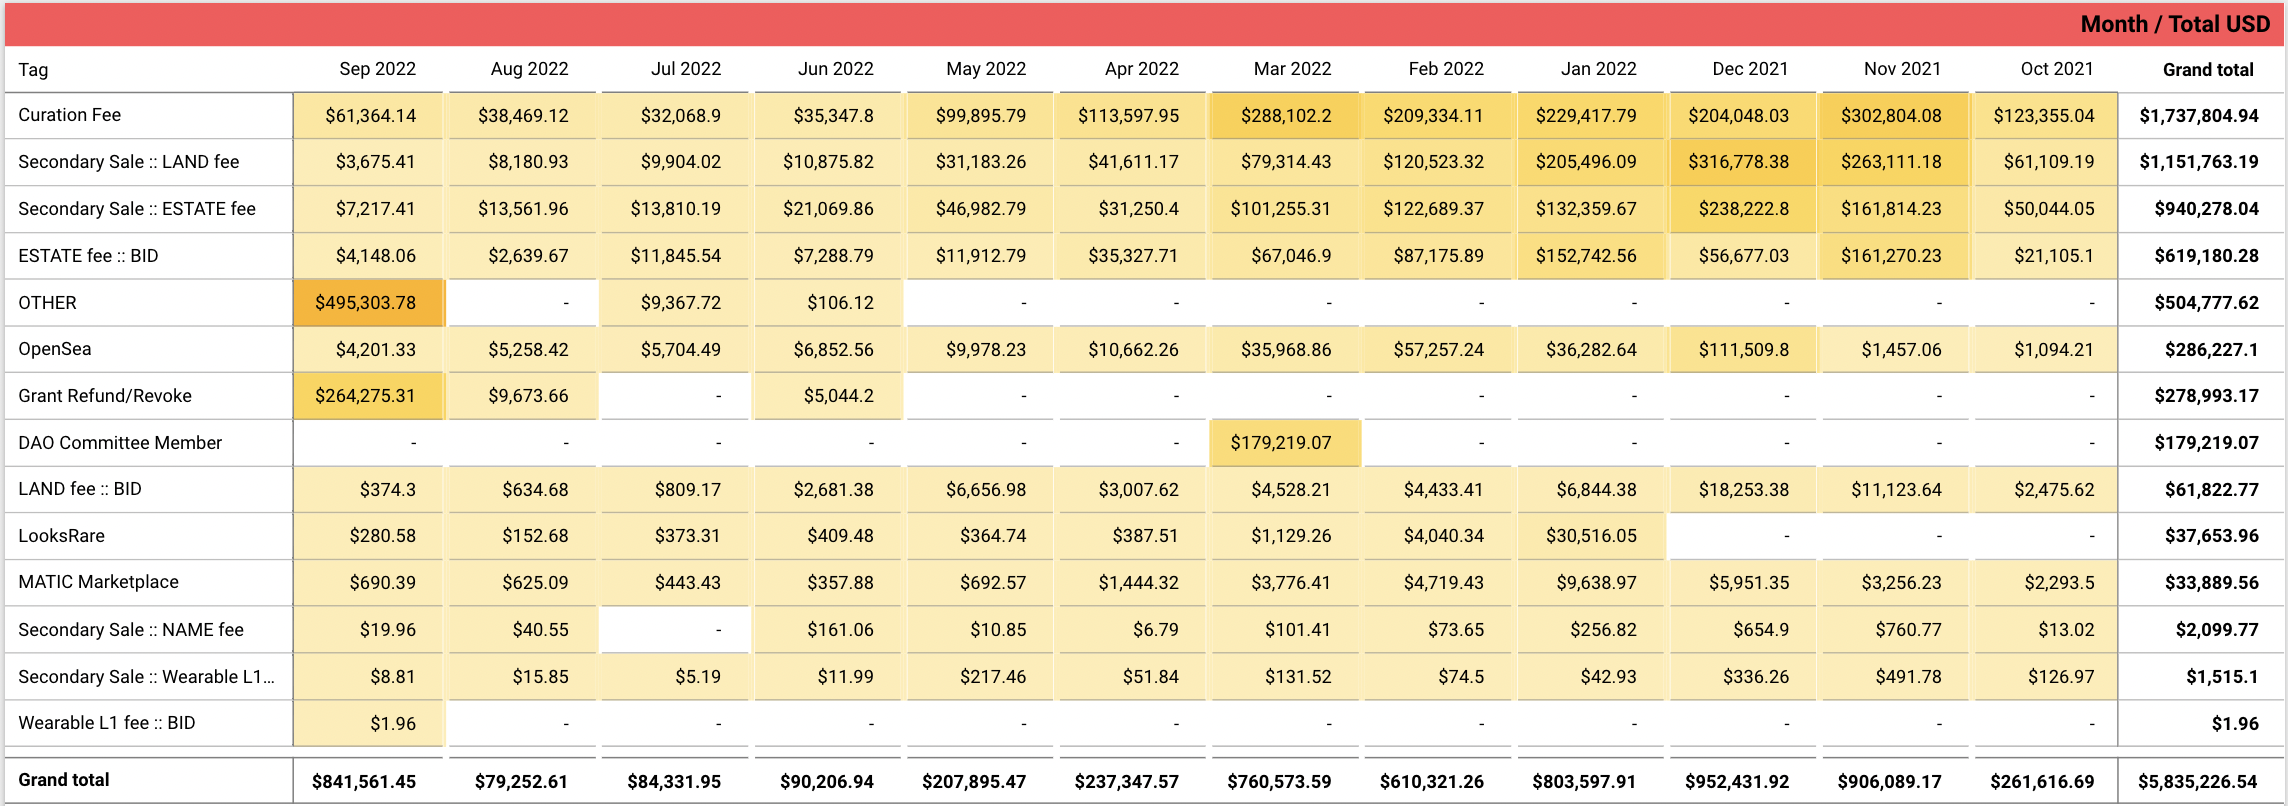
\includegraphics[width=\textwidth]{metrics/income.png}
  \caption{DAO revenue sources per month (*)}
  \label{fig:income}
\end{figure}
(*) Excluding DAO vesting contract\footnote{\url{https://vesting.decentraland.org/\#/0x7a3abf8897f31b56f09c6f69d074a393a905c1ac}}

Figure \ref{fig:expenses} shows the DAO expenses by month and by category, highlighting cells based on their values.
\begin{figure}[H]
  \centering
  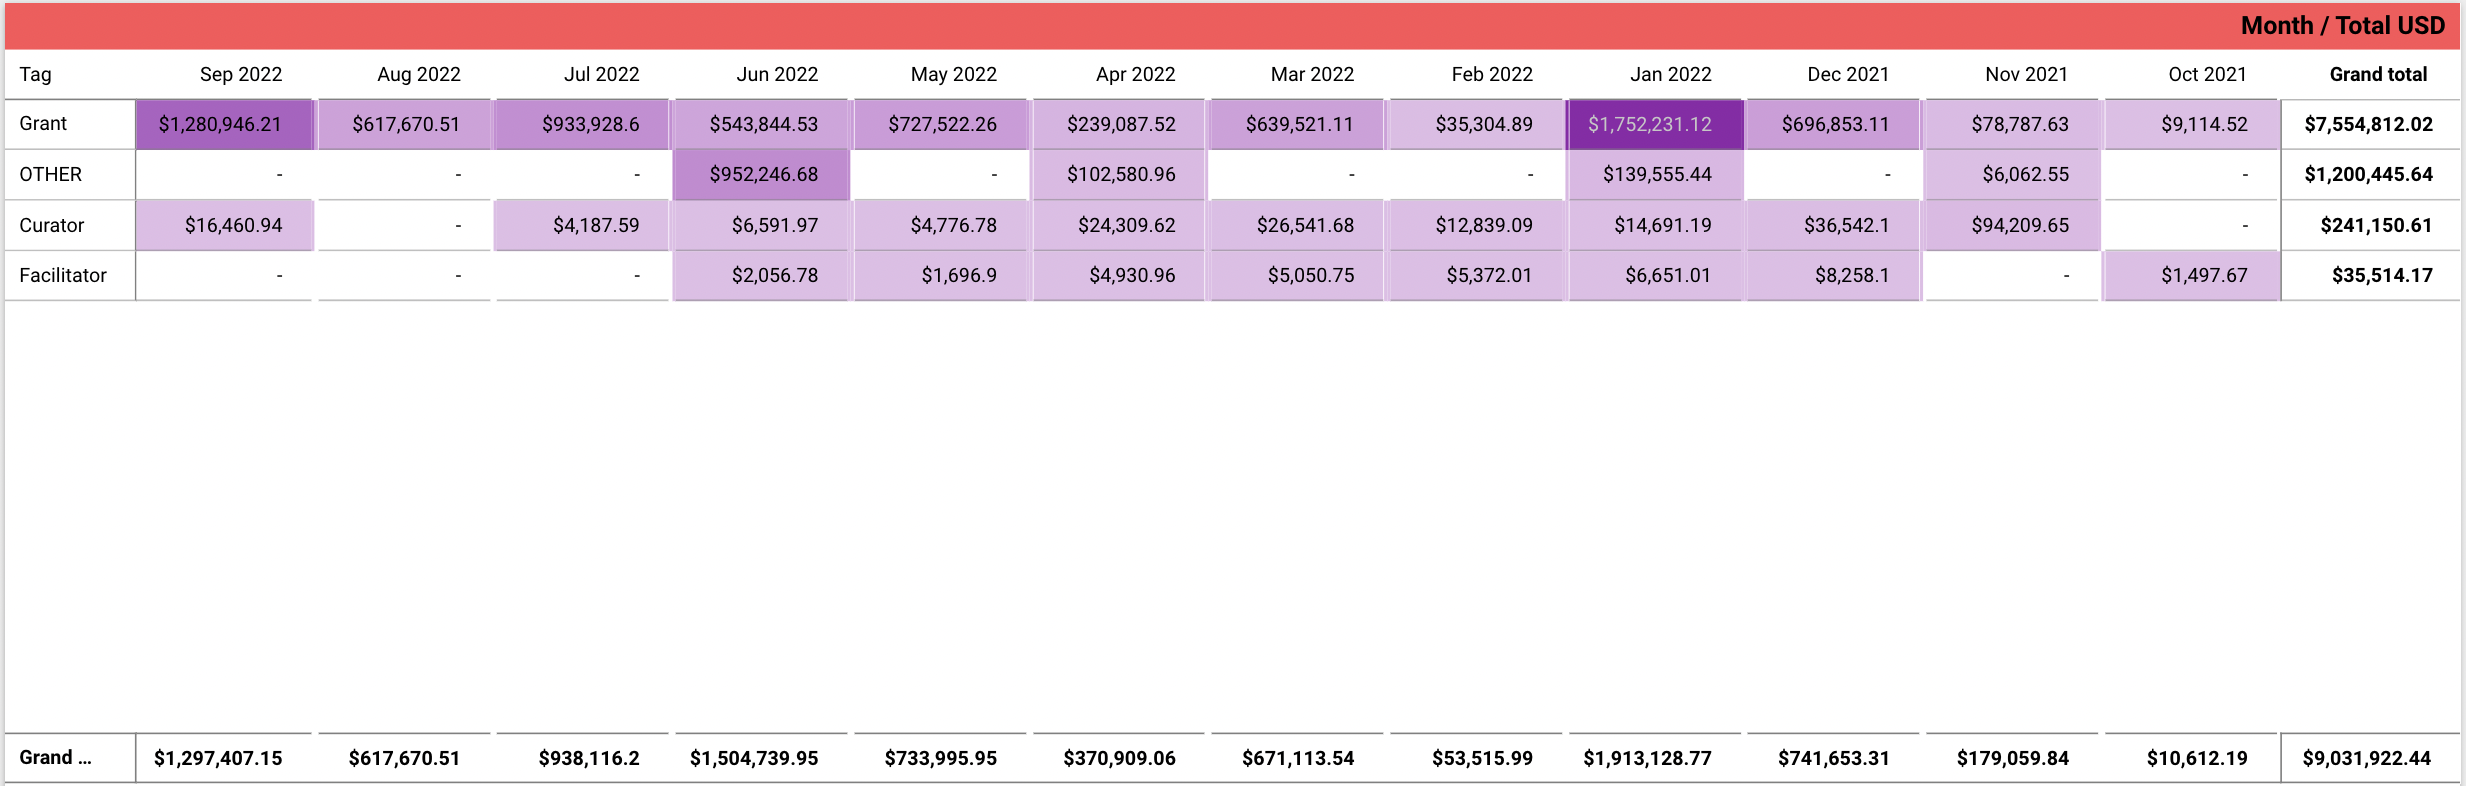
\includegraphics[width=\textwidth]{metrics/expenses.png}
  \caption{DAO expenses sources per month}
  \label{fig:expenses}
\end{figure}

Table \ref{table:fees} shows to date, the number of transactions made by the DAO wallets in different periods, how much was paid in total in gas fees (expressed in US dollars) and also the average of said values.
\begin{center}
  \begin{table}[H]
    \begin{tabular}{ | m{8em} | m{10em} | m{6em} | m{15em} | }
      \hline
      \textbf{Time period} & \textbf{Transactions amount} & \textbf{Total USD} & \textbf{Average USD per transaction} \\ 
      \hline
      Last 30 days &	10 &	\$180.03 &	\$18 \\
      \hline
      Last 60 days &	18 &	\$333.73 &	\$18.54 \\
      \hline
      Last 6 months &	51 &	\$1,081.57 &	\$21.21 \\
      \hline
      Last year &	86 &	\$6,164.27 &	\$71.68 \\
      \hline
    \end{tabular}
    \caption{Transaction fees paid by DAO wallets}
    \label{table:fees}
  \end{table}
\end{center}

\section{Wearable curations}

Figure \ref{fig:curations} shows how many wearable curations each curator made per month. Each color represents the curator's wallet address.
\begin{figure}[H]
  \centering
  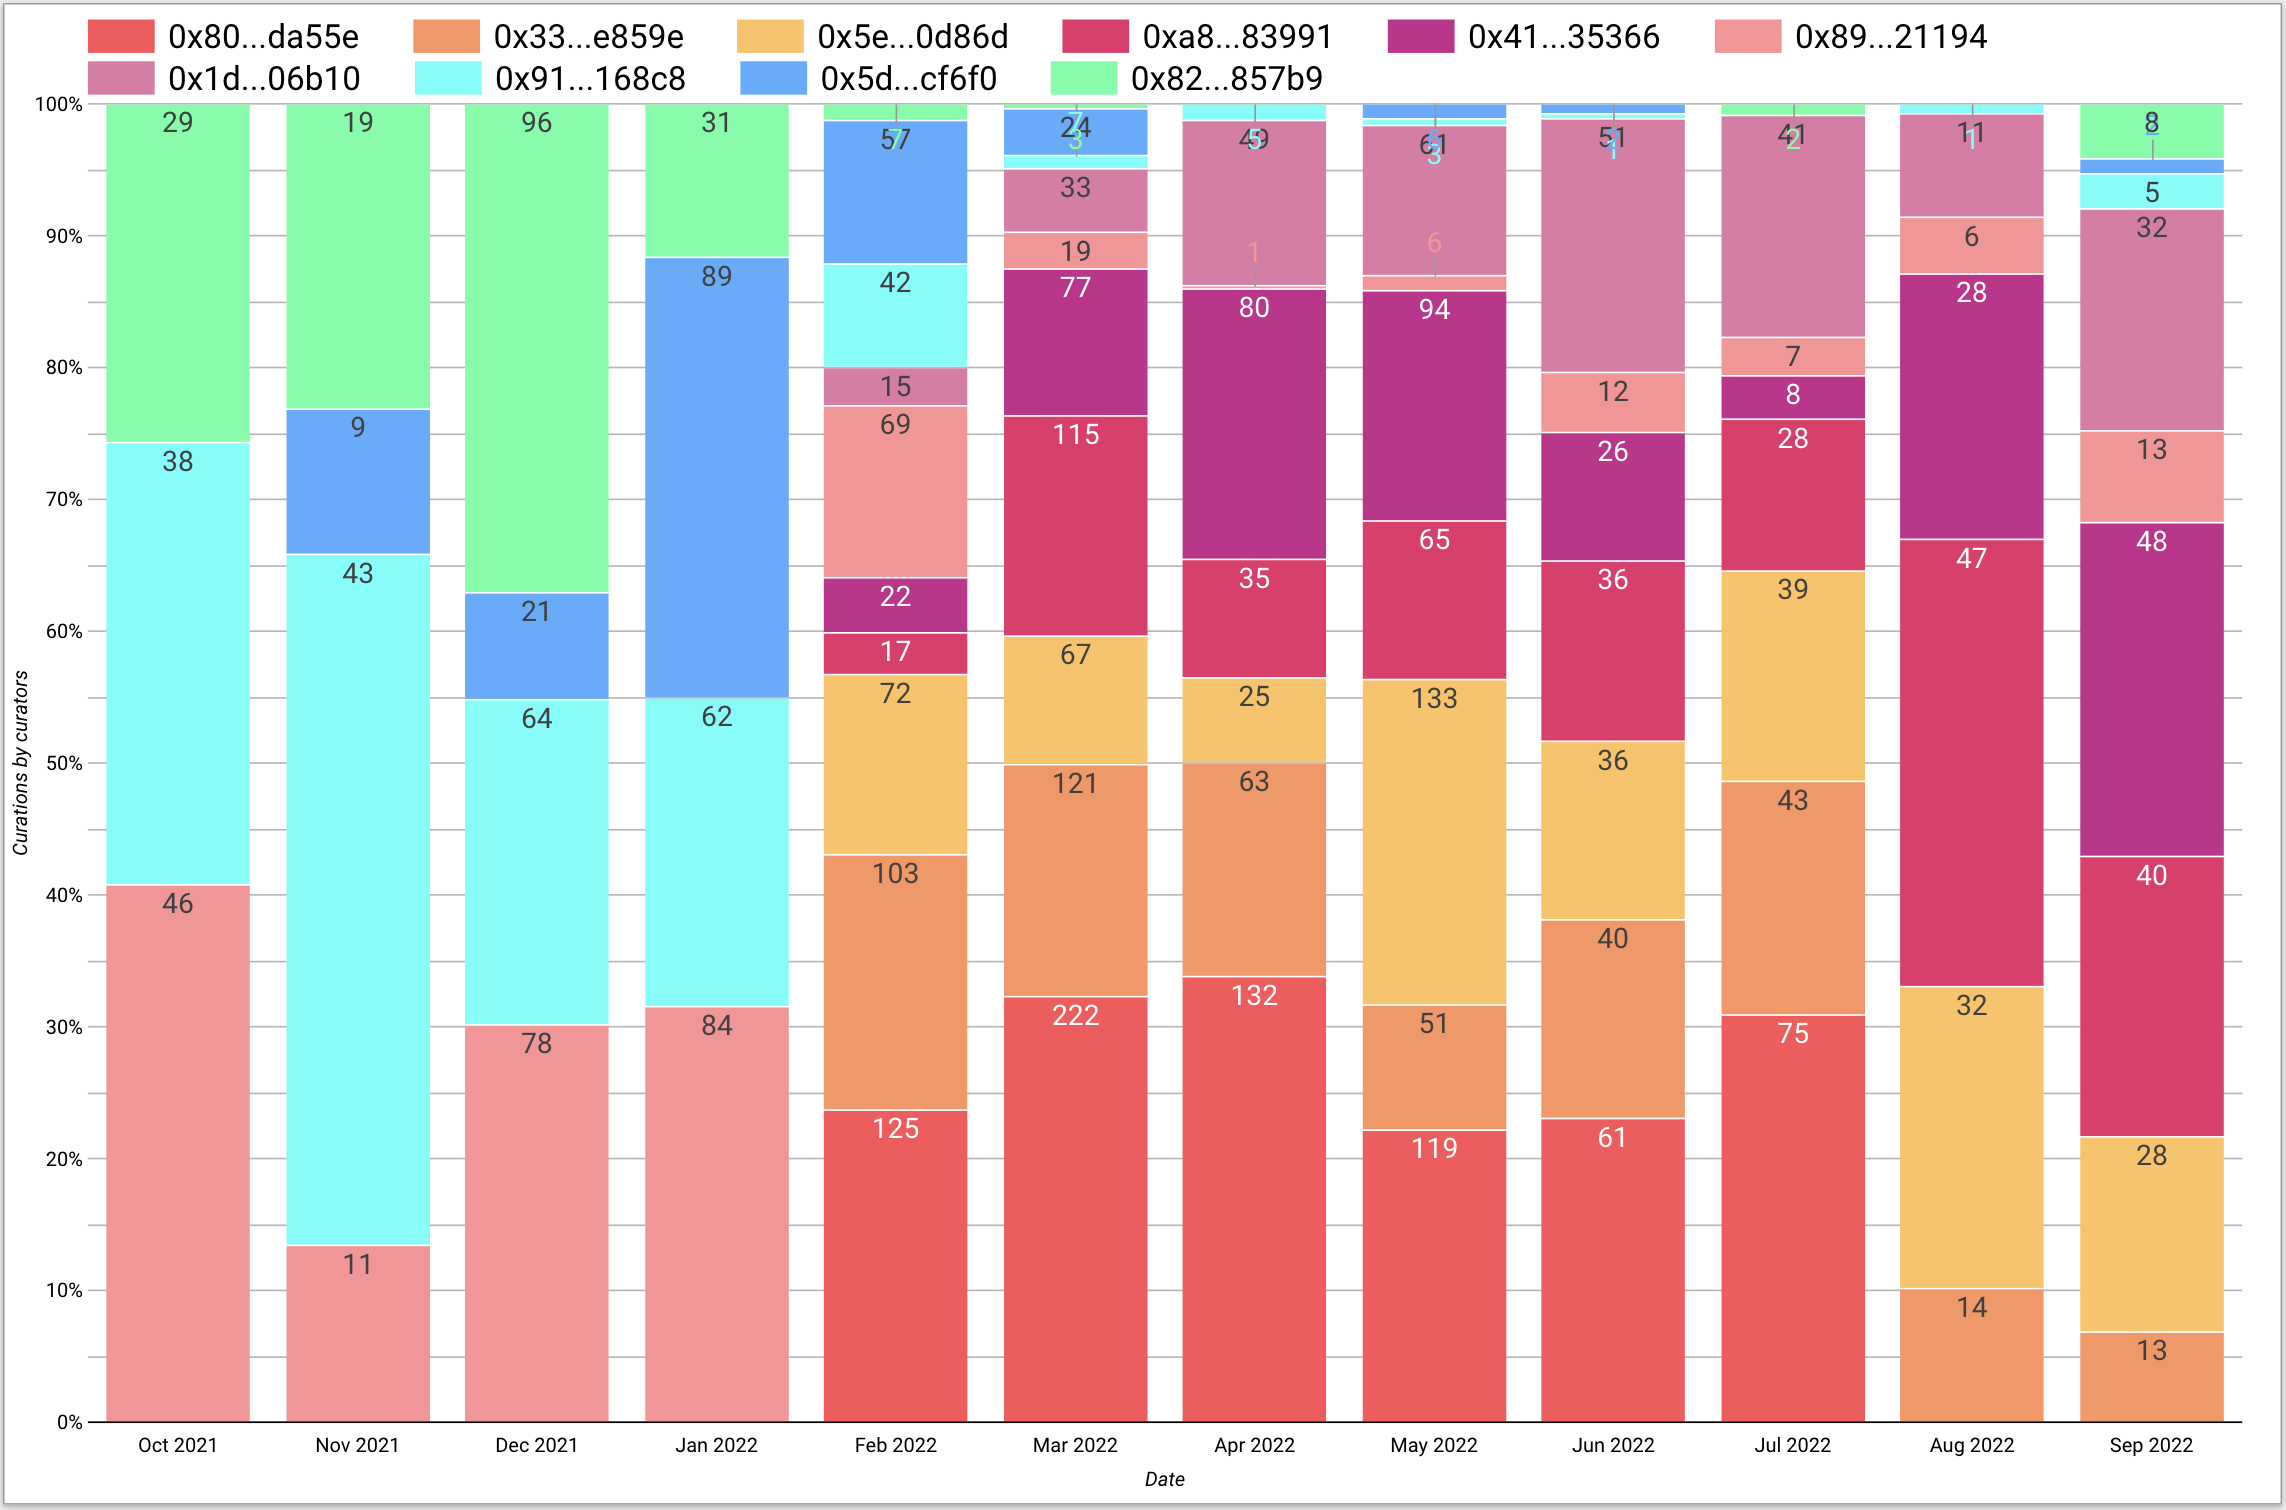
\includegraphics[width=\textwidth]{metrics/curations.png}
  \caption{Curations made by curators per month}
  \label{fig:curations}
\end{figure}

Figure \ref{fig:submission_fees} shows how much money the DAO received per month (expressed in U.S. dollars at the then current value) from users for wearable curations.
\begin{figure}[H]
  \centering
  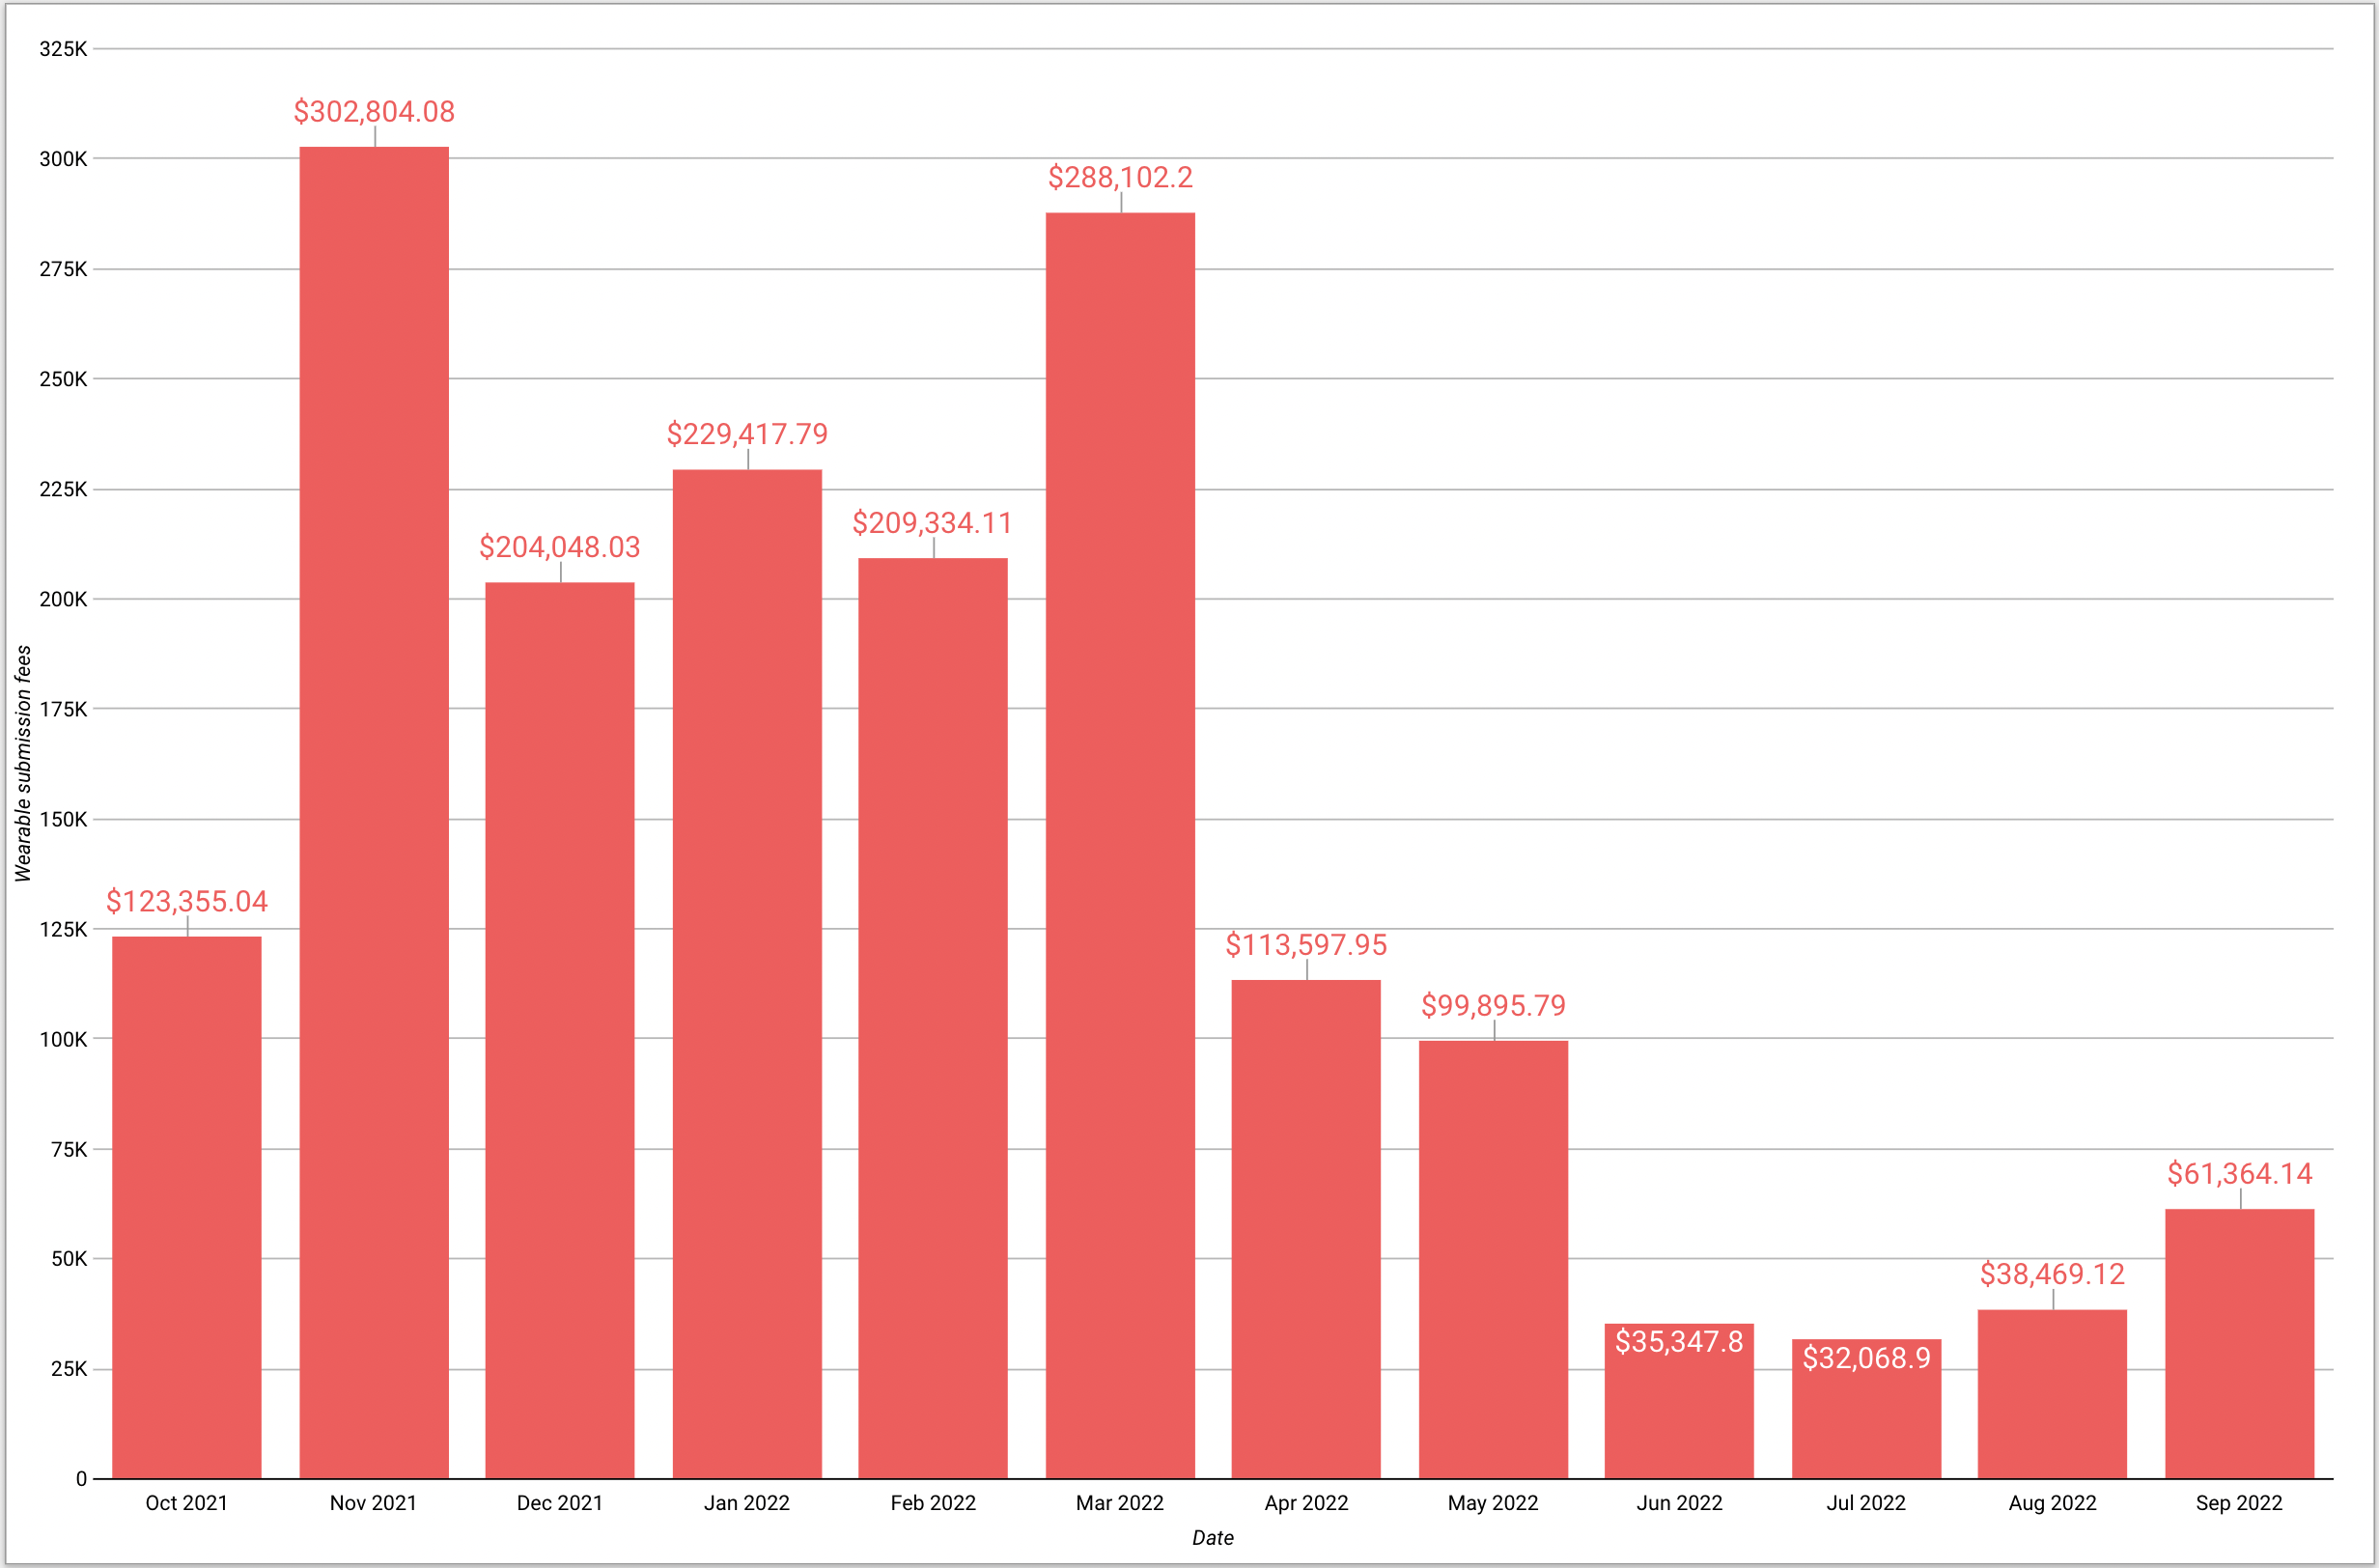
\includegraphics[width=\textwidth]{metrics/submission_fees.png}
  \caption{Wearable submission fees per month}
  \label{fig:submission_fees}
\end{figure}

Figure \ref{fig:curators_pay} shows the amount of money paid to the curators per month (expressed in U.S. dollars at the then current value) for curations performed.
\begin{figure}[H]
  \centering
  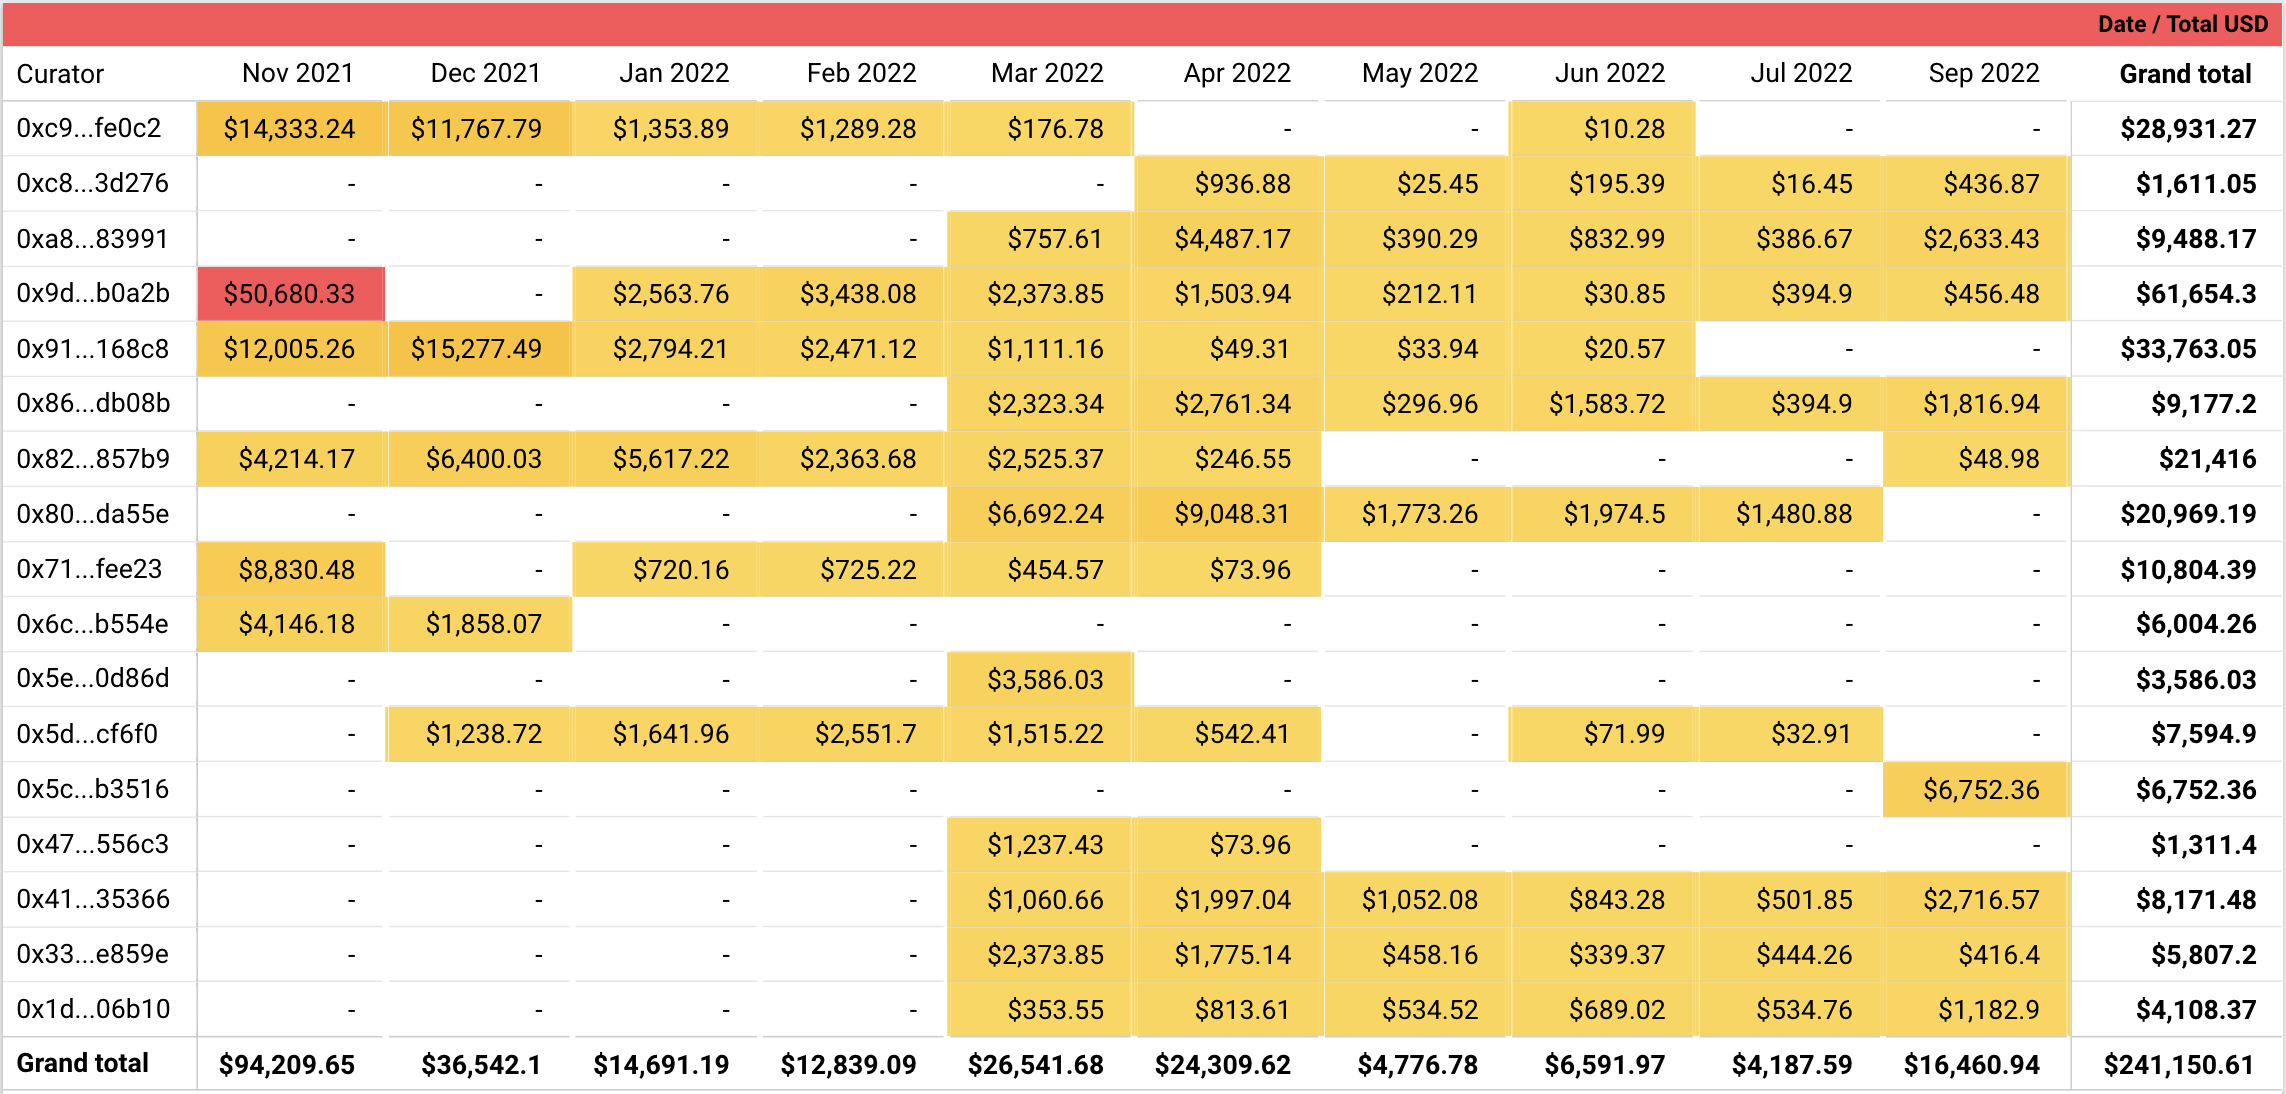
\includegraphics[width=\textwidth]{metrics/curators_pay.png}
  \caption{Curators pay per month}
  \label{fig:curators_pay}
\end{figure}

Figure \ref{fig:day_difference} shows by month, the average number of days difference between the submission of wearables for curation and the curation by the curators. The lower the number, the faster the curation happens.
\begin{figure}[H]
  \centering
  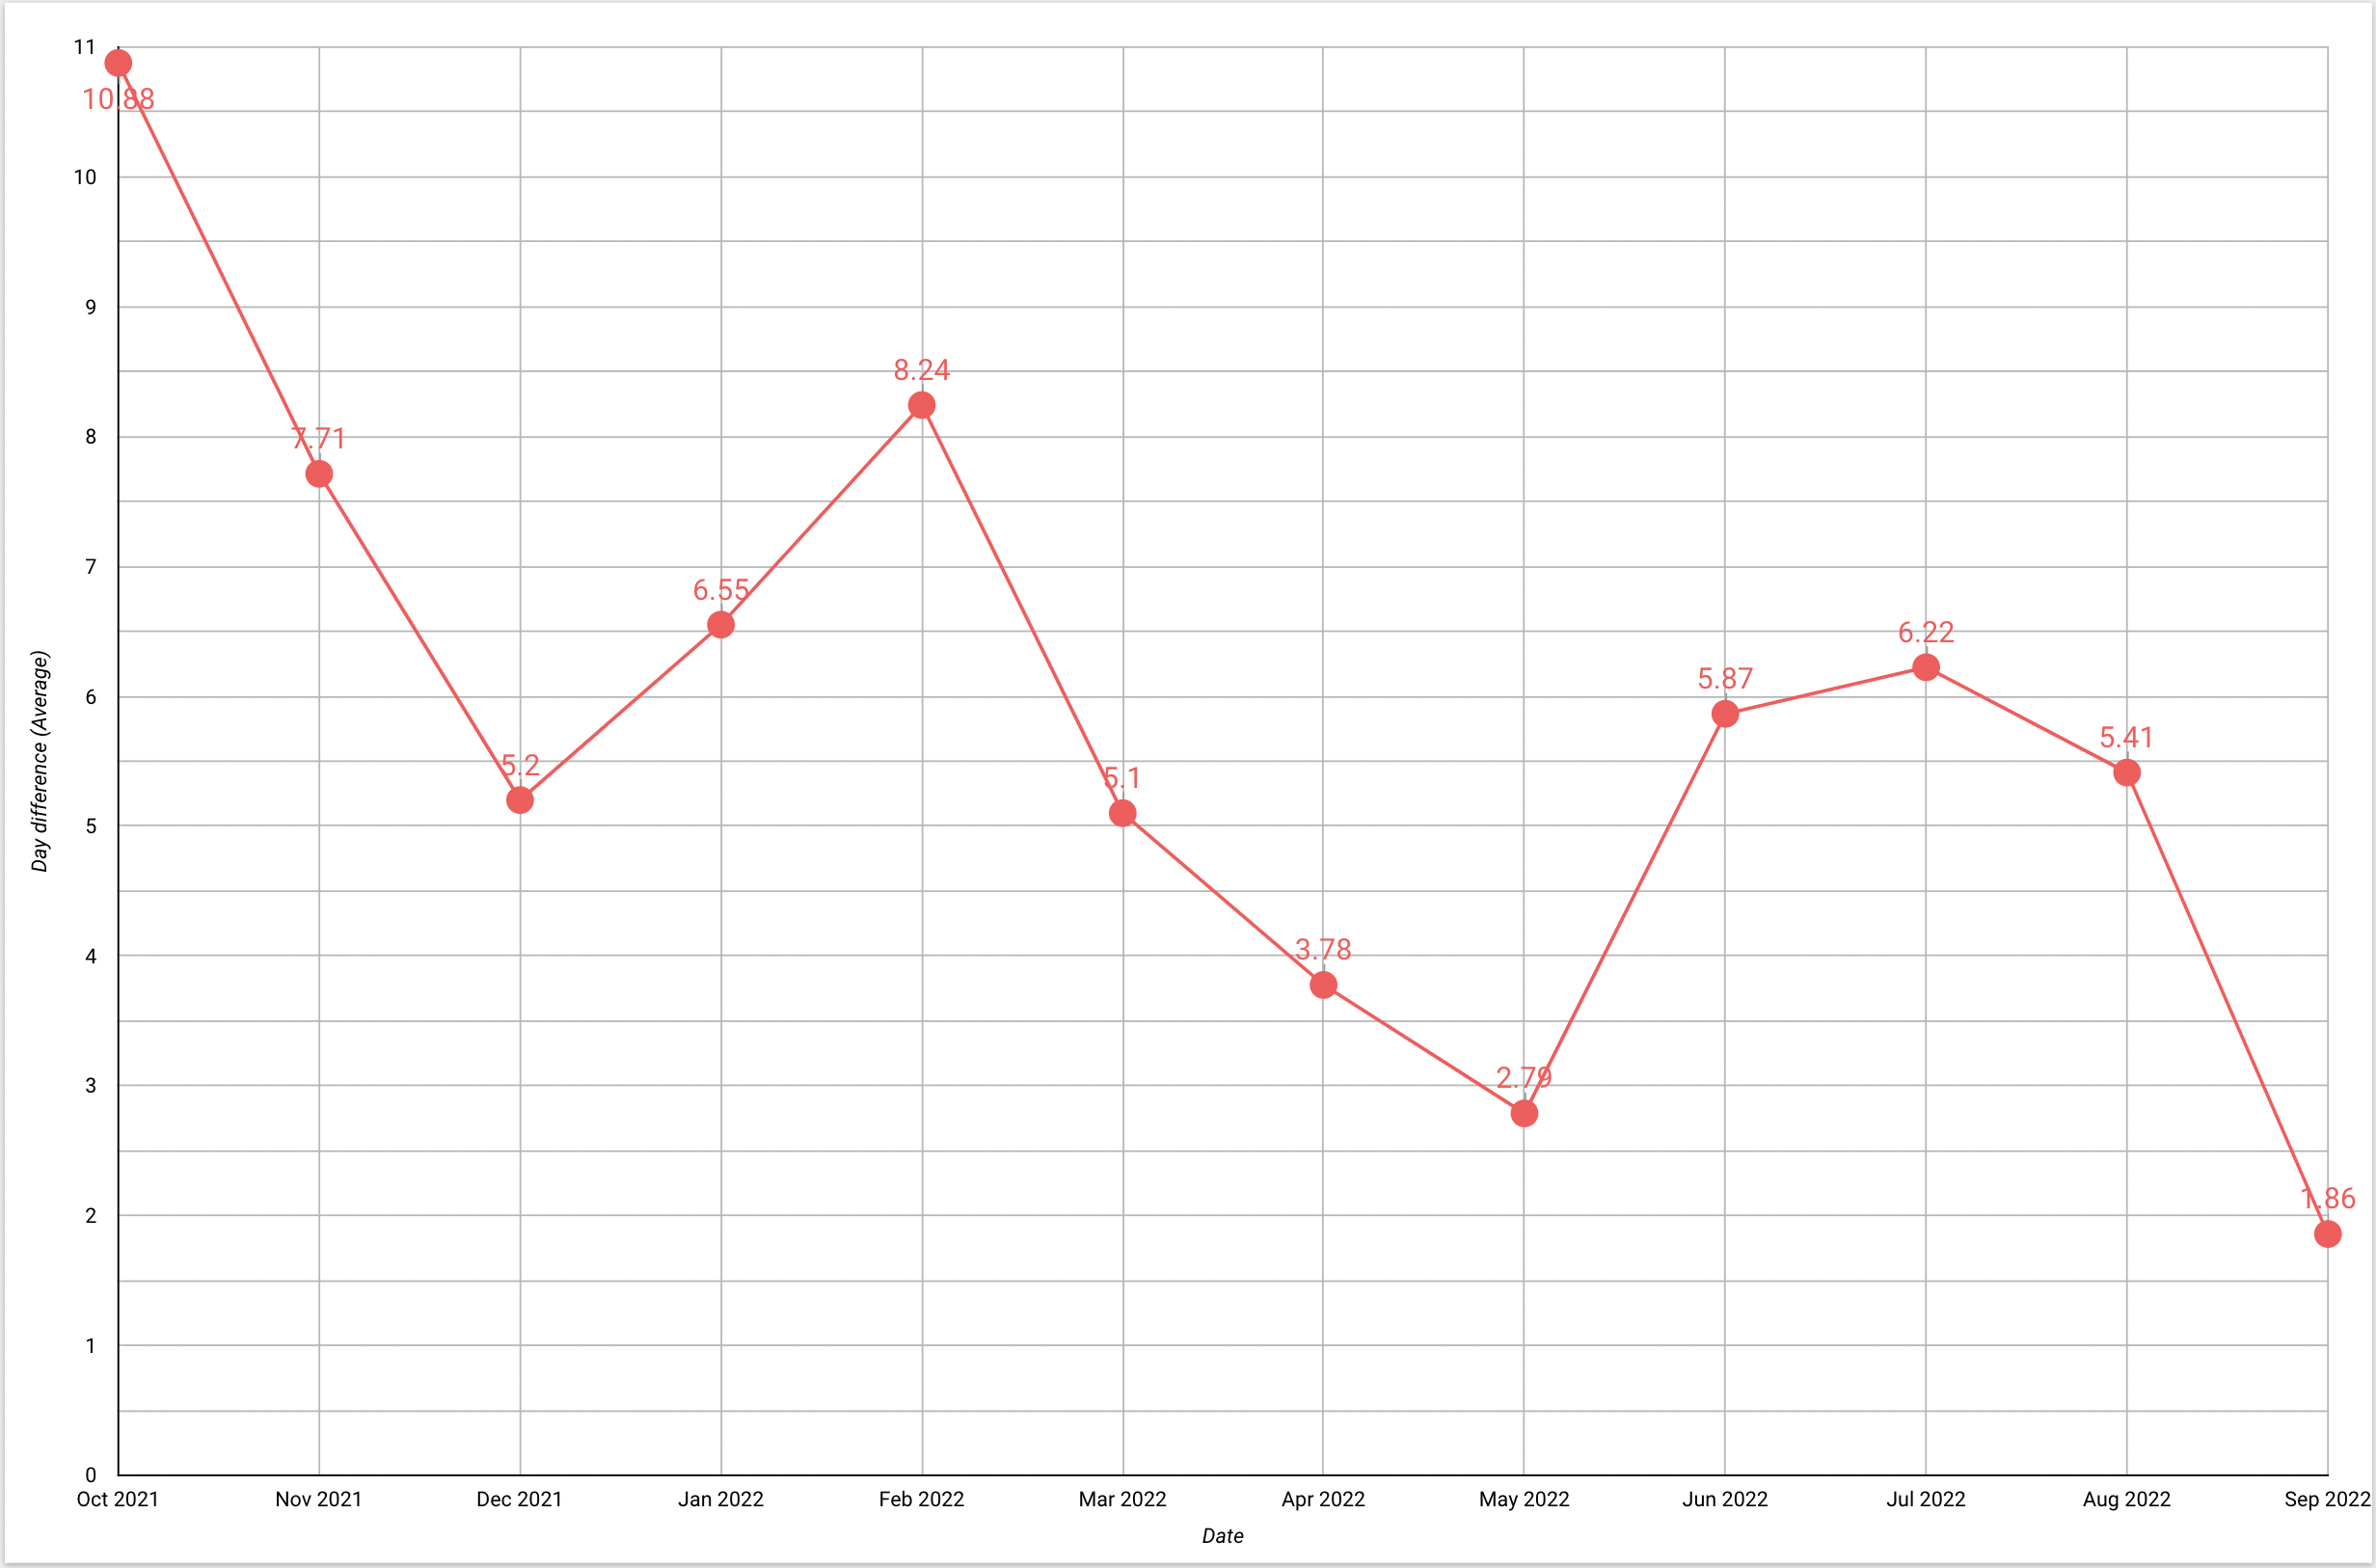
\includegraphics[width=\textwidth]{metrics/day_difference.png}
  \caption{Average day difference between collection submission and curator review}
  \label{fig:day_difference}
\end{figure}

Figure \ref{fig:rarity_distribution} shows how the rarity of wearables in circulation to date is distributed.
\begin{figure}[H]
  \centering
  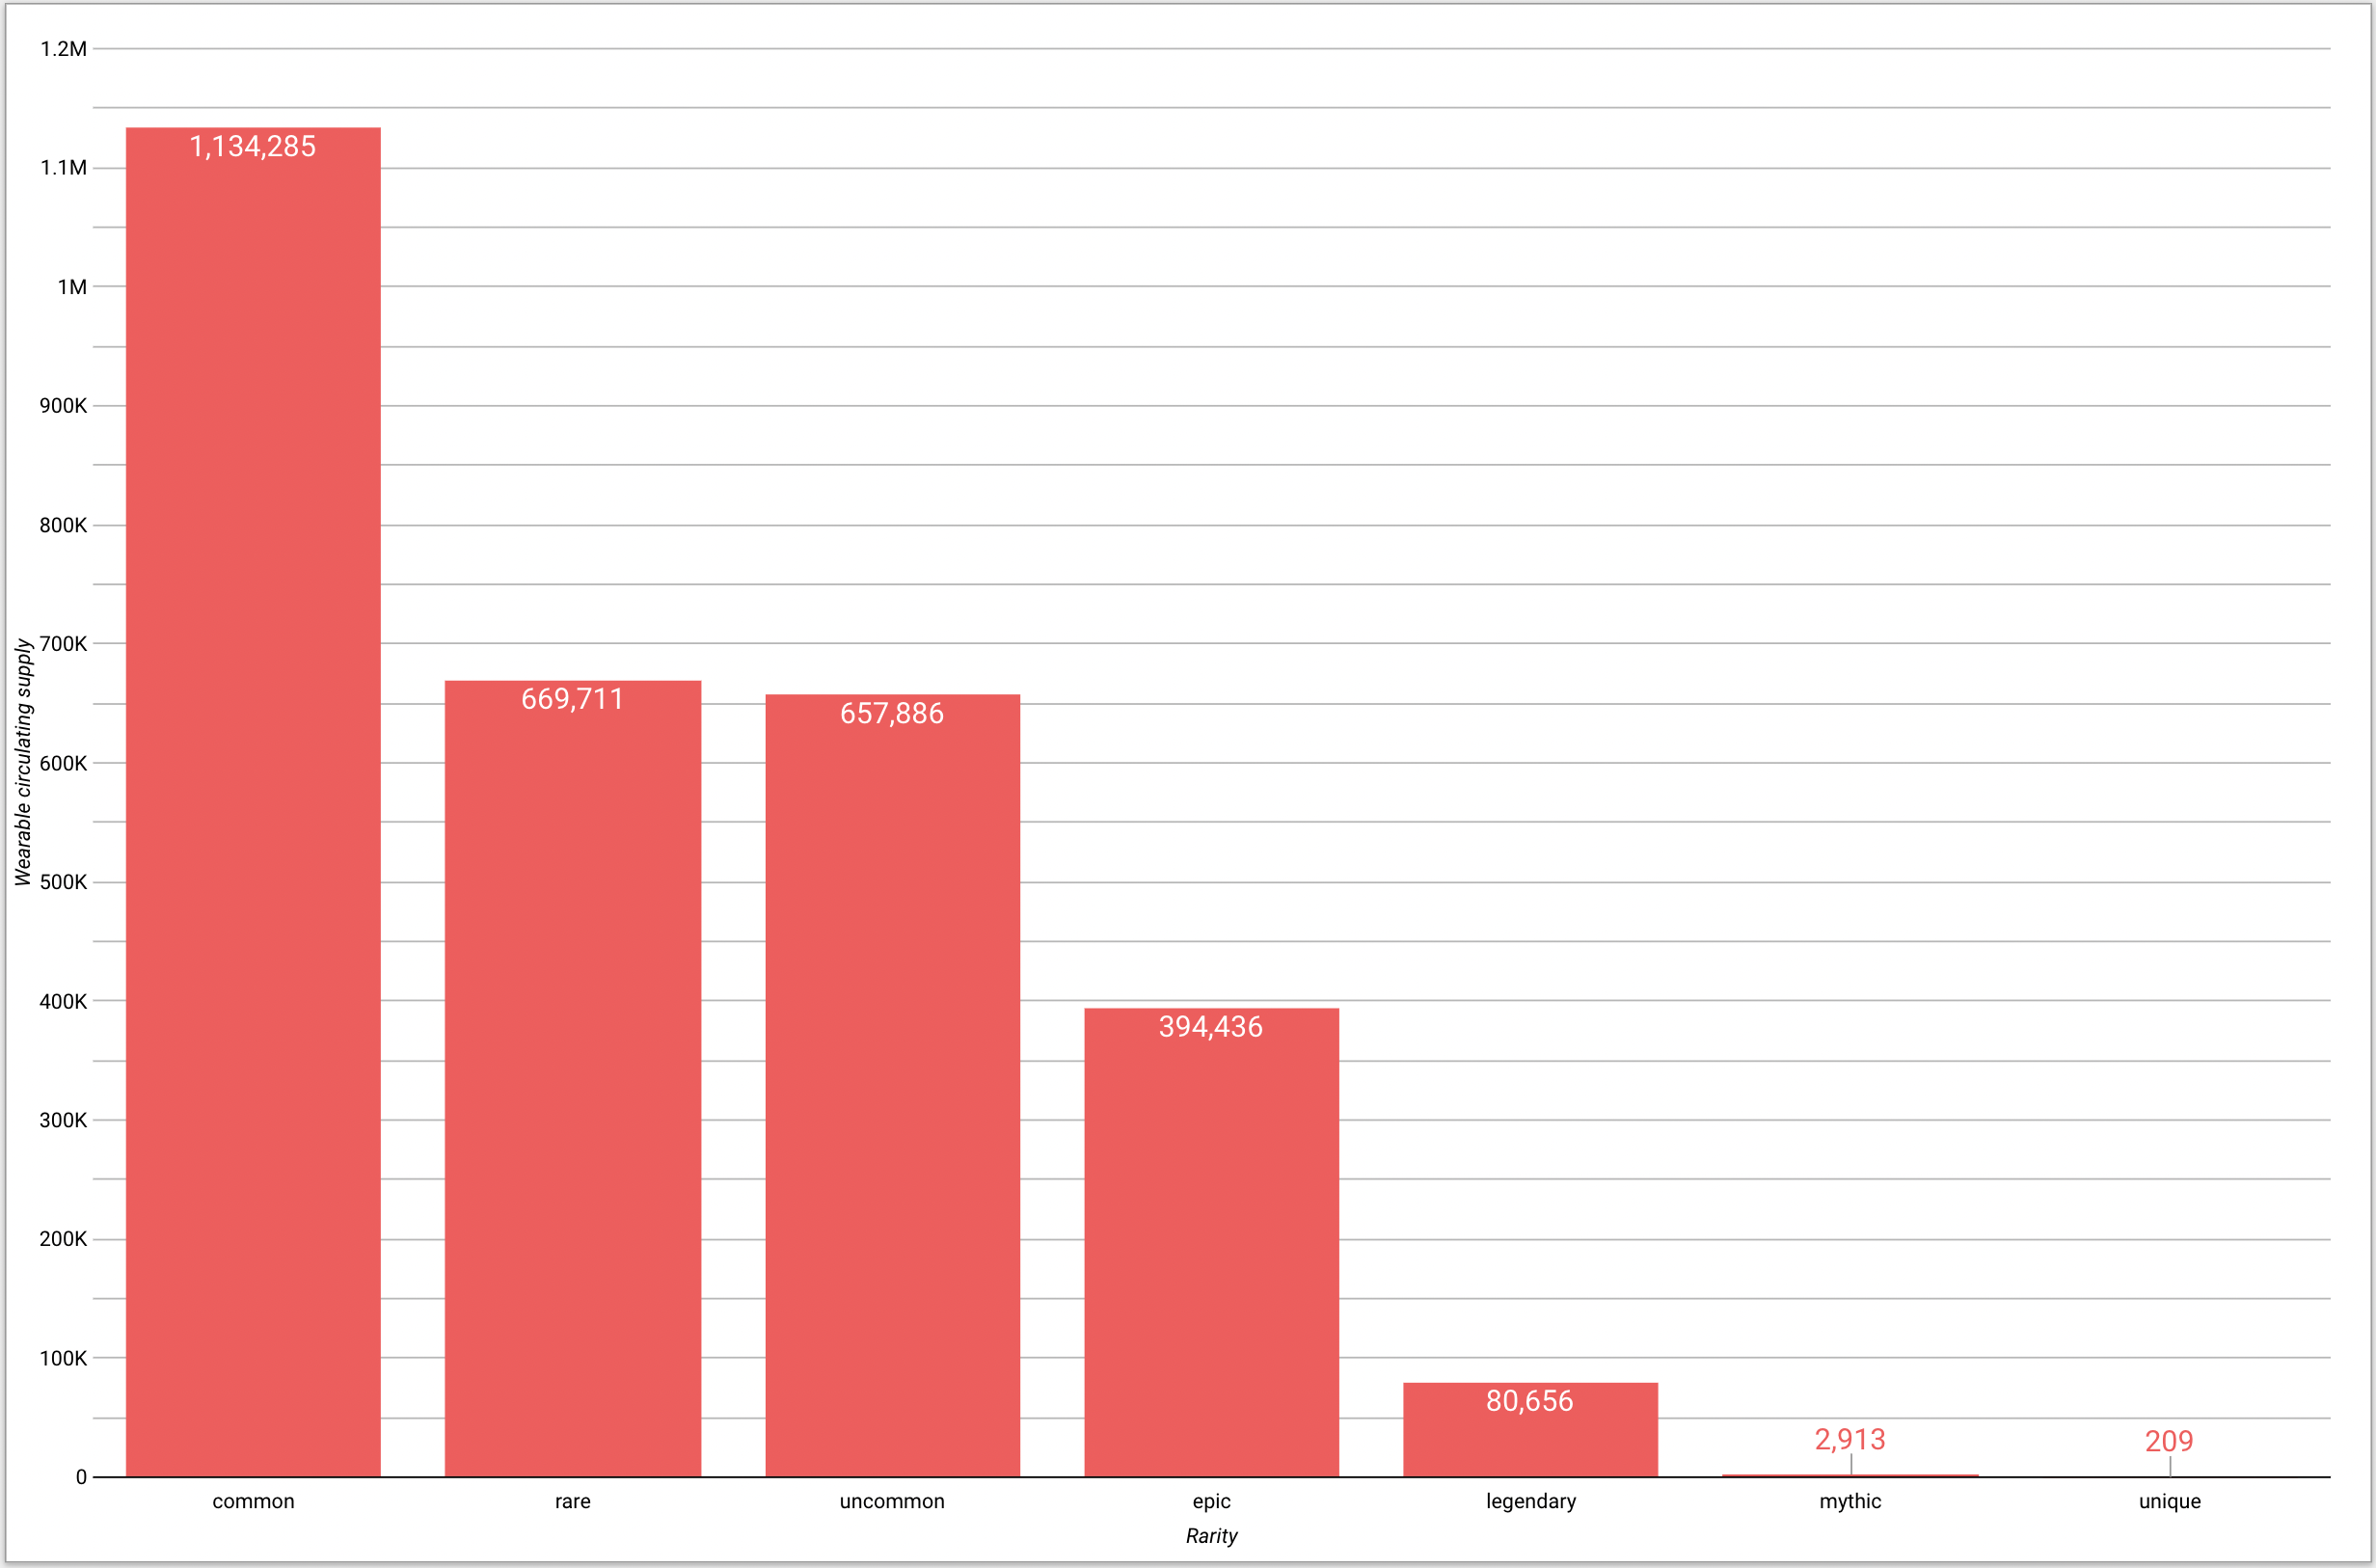
\includegraphics[width=\textwidth]{metrics/rarity_distribution.png}
  \caption{Distribution of the rarity of circulating wearables}
  \label{fig:rarity_distribution}
\end{figure}

Figure \ref{fig:sales_fees} shows the total fees received by the DAO per month for Decentraland assets transactions (wearables, LANDs and NAMES).
\begin{figure}[H]
  \centering
  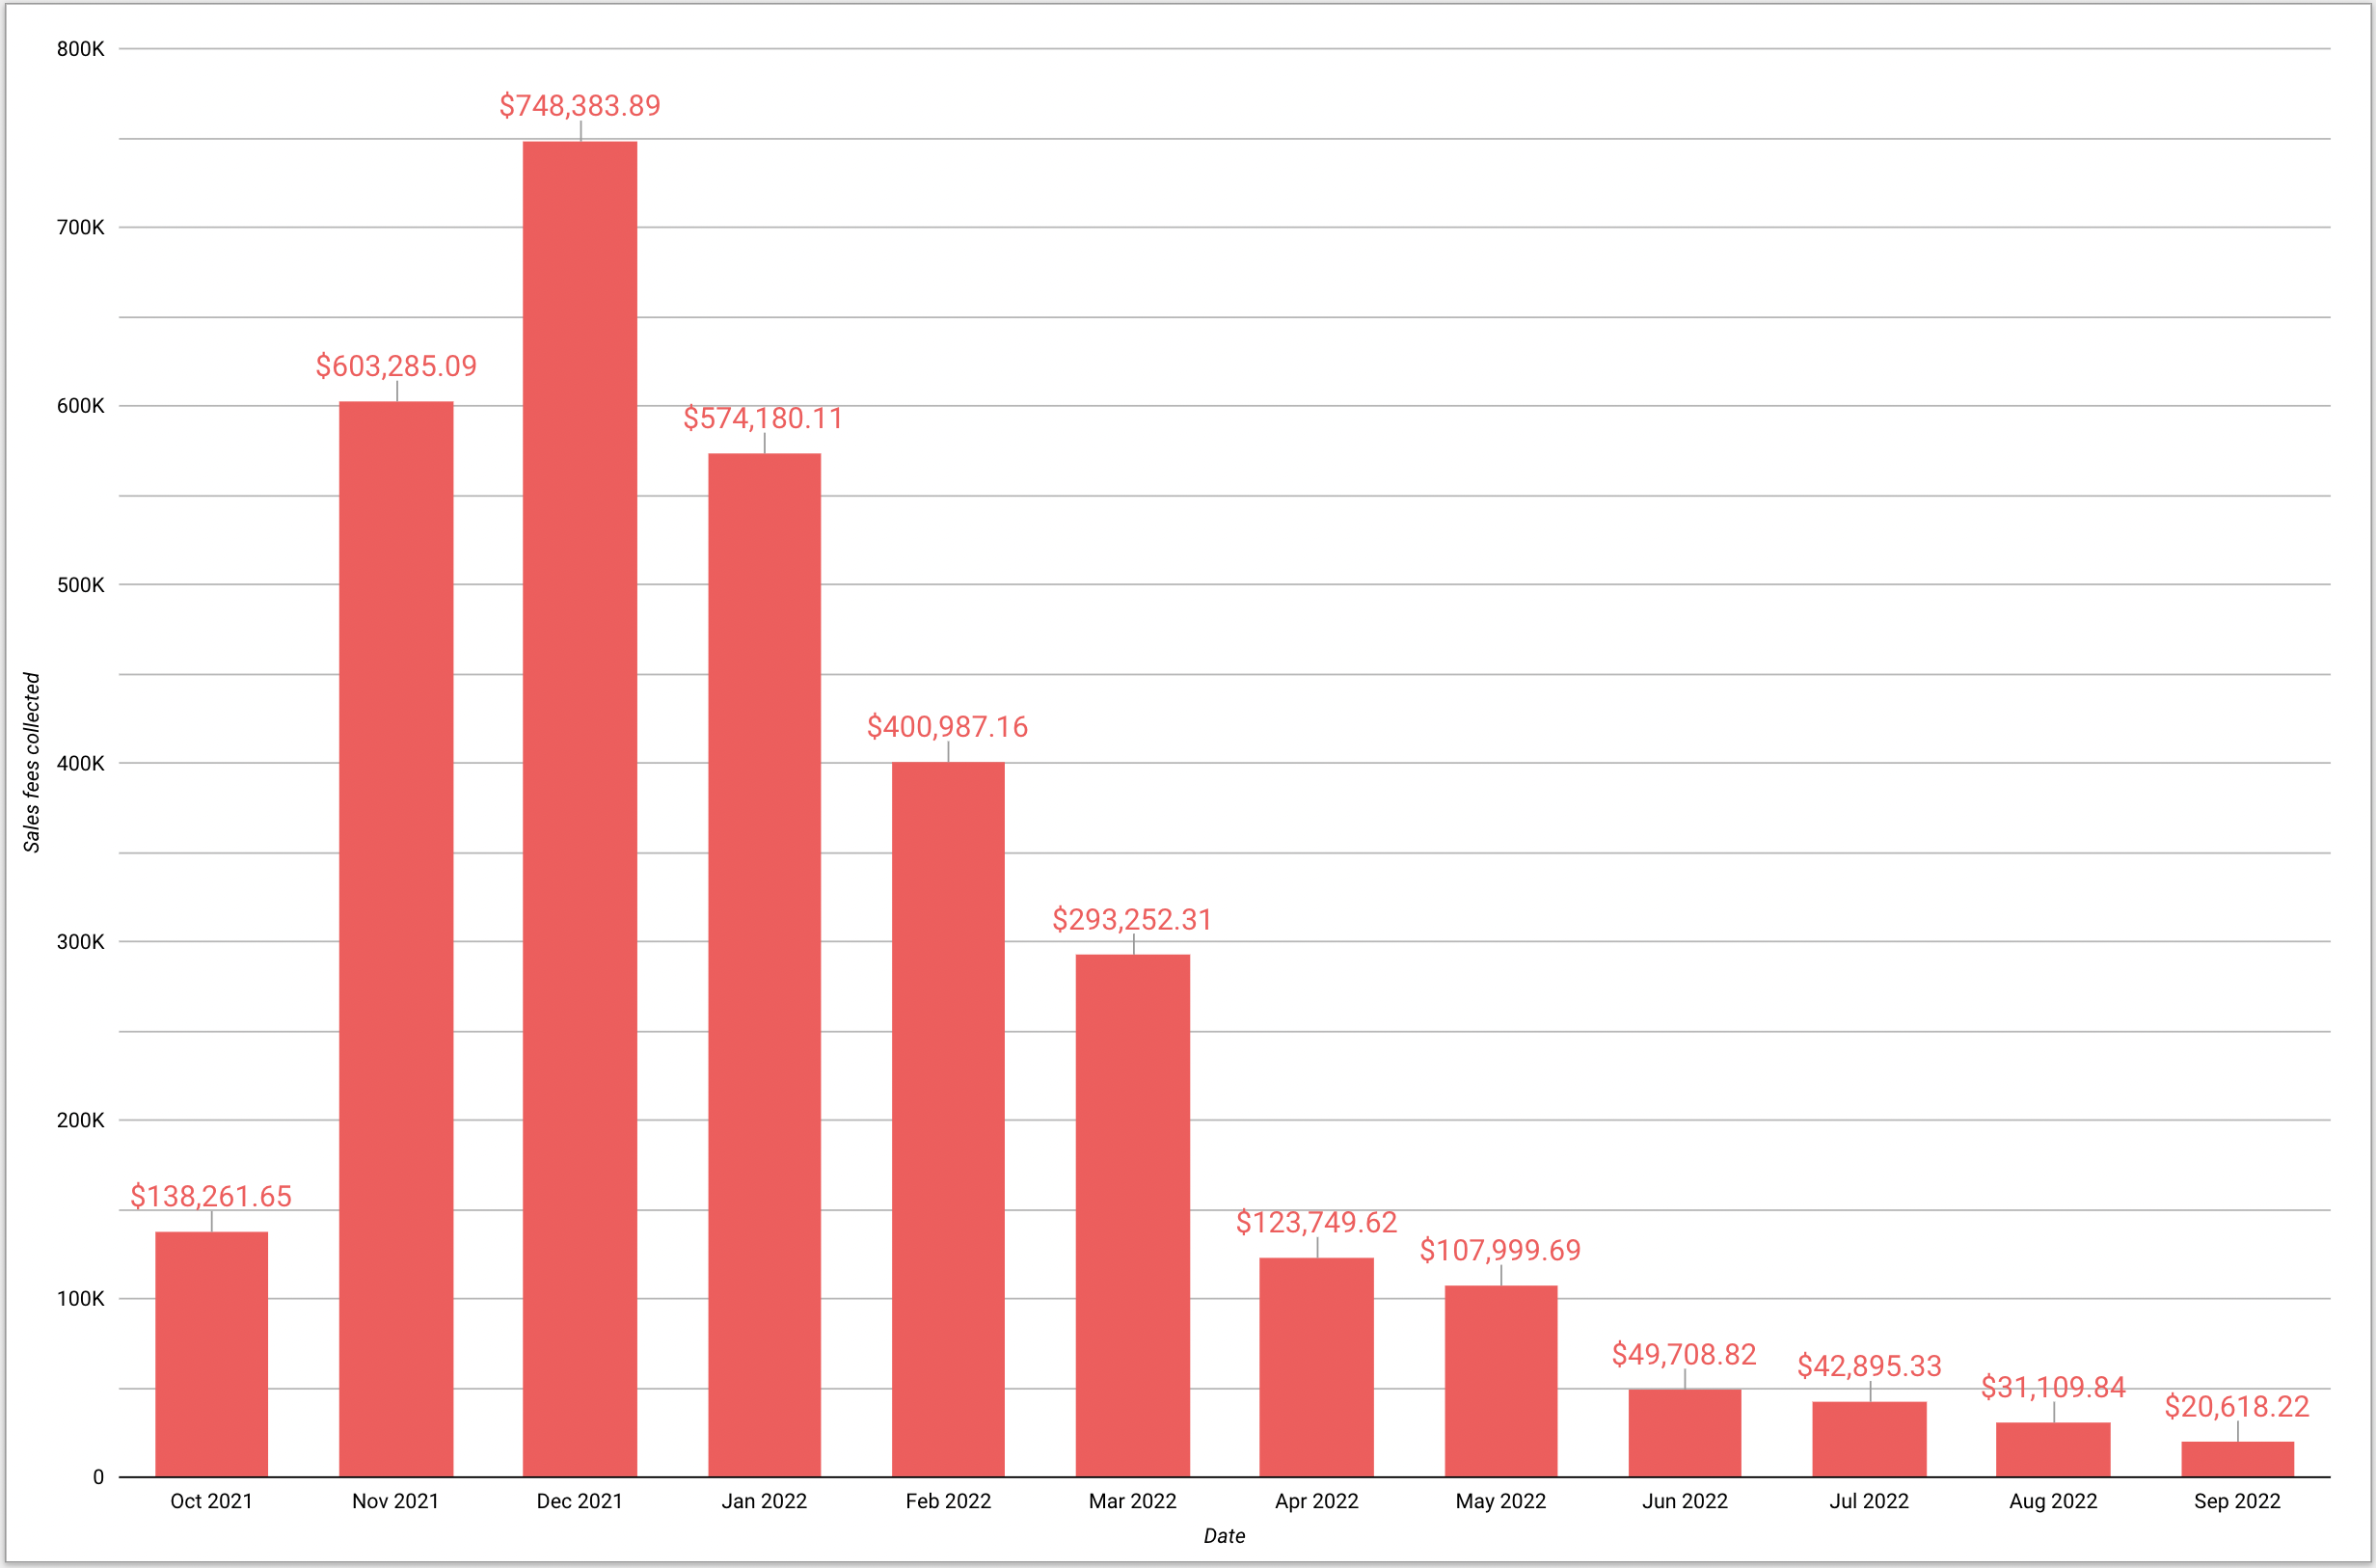
\includegraphics[width=\textwidth]{metrics/sales_fees.png}
  \caption{Sales fees collected per month (including LAND and NAMES)}
  \label{fig:sales_fees}
\end{figure}

\section{DAO Members}
Total unique DAO members (to date): \textbf{3.226} \\

Figure \ref{fig:active_members} shows the total number of active DAO members by month. This count is done by considering unique votes per month from the different addresses participating in the DAO.
\begin{figure}[H]
  \centering
  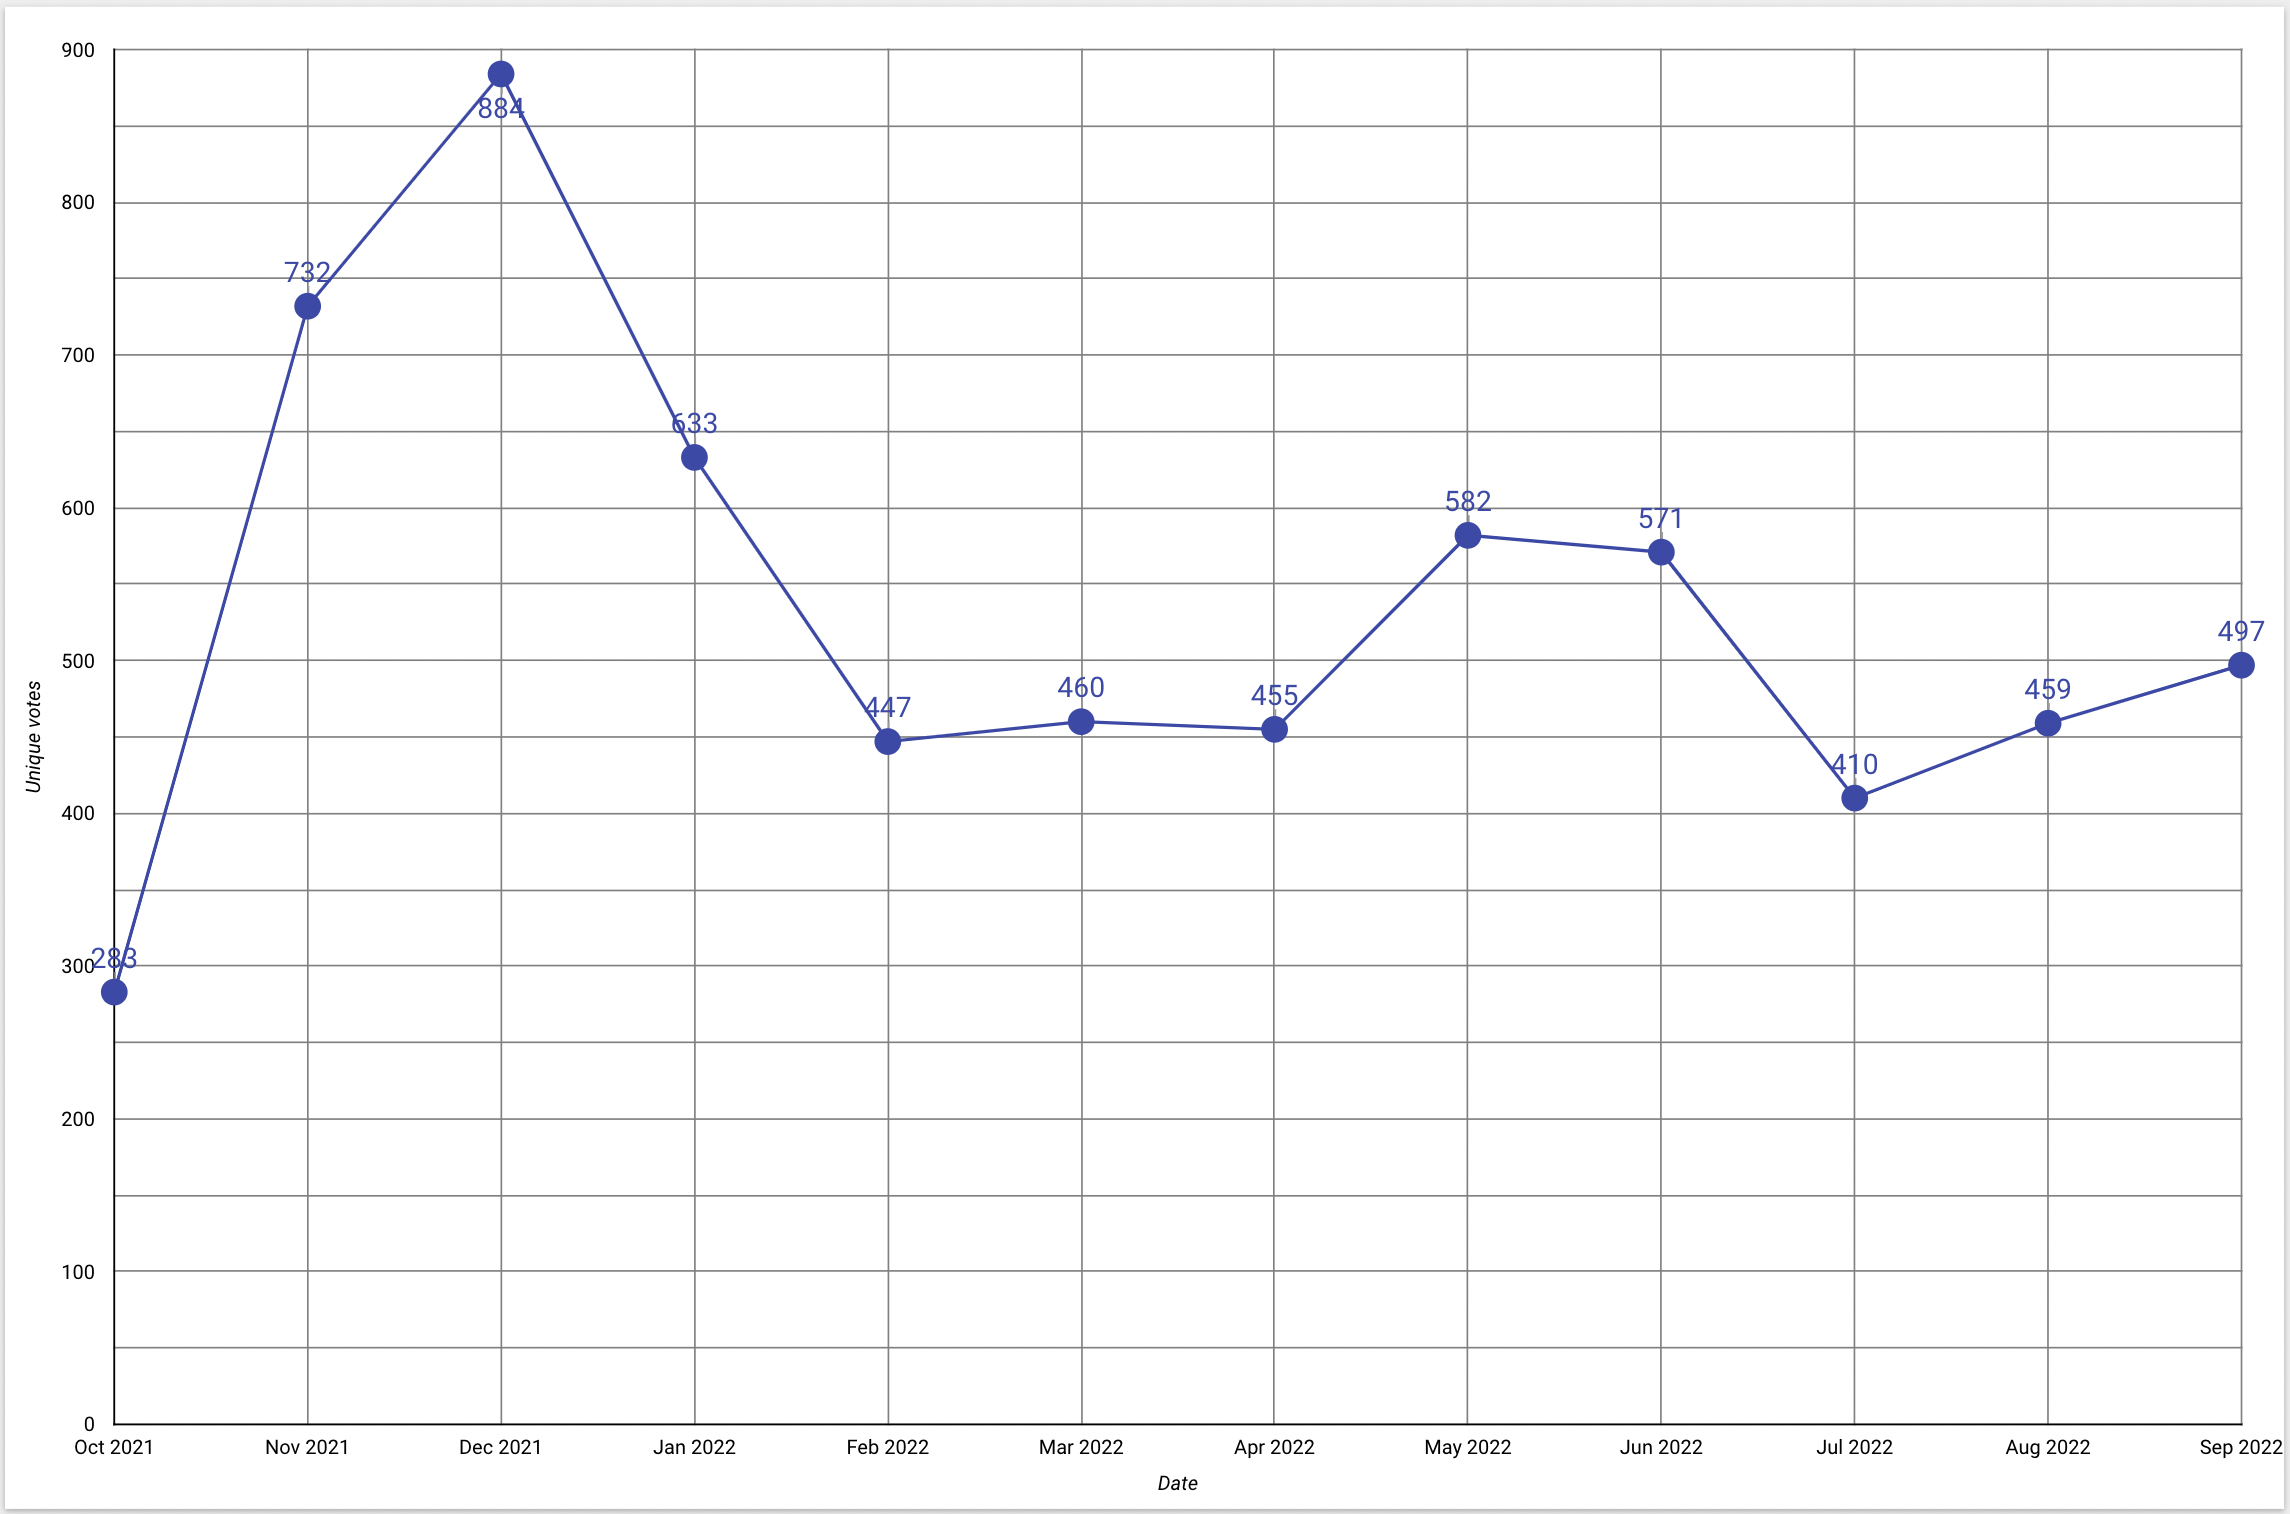
\includegraphics[width=\textwidth]{metrics/active_members.png}
  \caption{Active DAO members per month}
  \label{fig:active_members}
\end{figure}

Figure \ref{fig:delegation_ratio} shows the distribution of members participating in the DAO who have or have not delegated their voting power to date.
\begin{figure}[H]
  \centering
  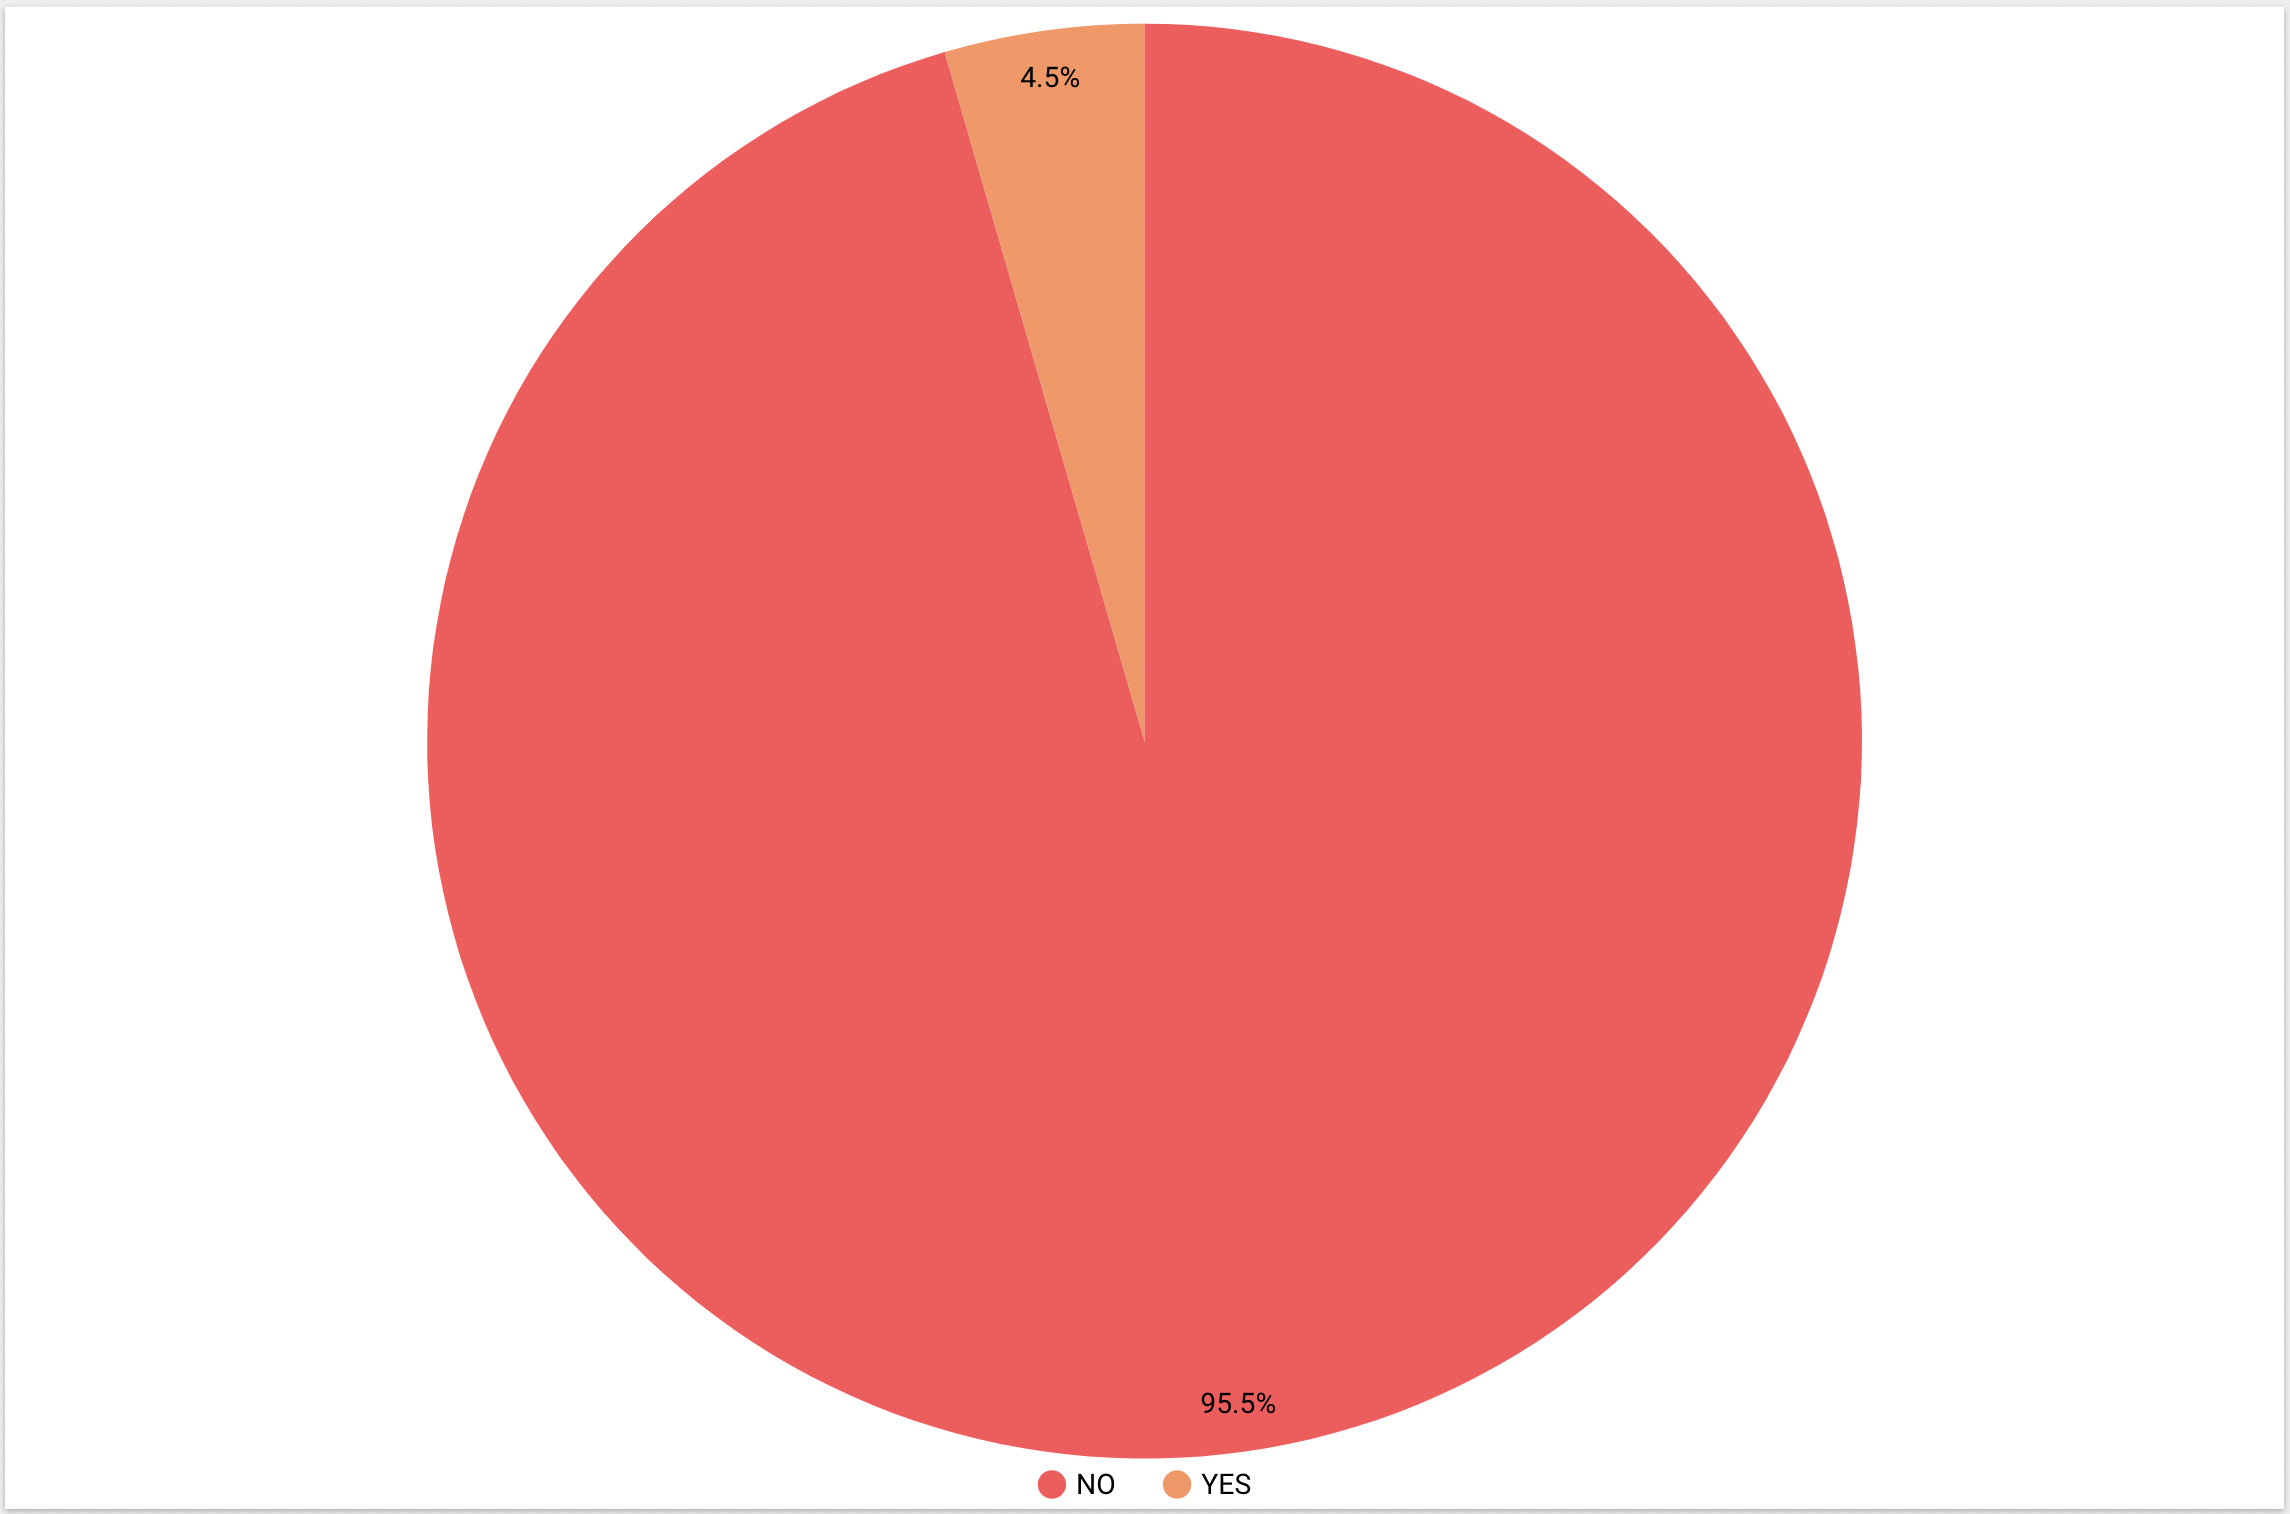
\includegraphics[width=\textwidth]{metrics/delegation_ratio.png}
  \caption{Distribution of members who have or have not delegated their voting power}
  \label{fig:delegation_ratio}
\end{figure}

Figure \ref{fig:top_voters} shows the historical top 25 addresses that voted the most on DAO proposals.
\begin{figure}[H]
  \centering
  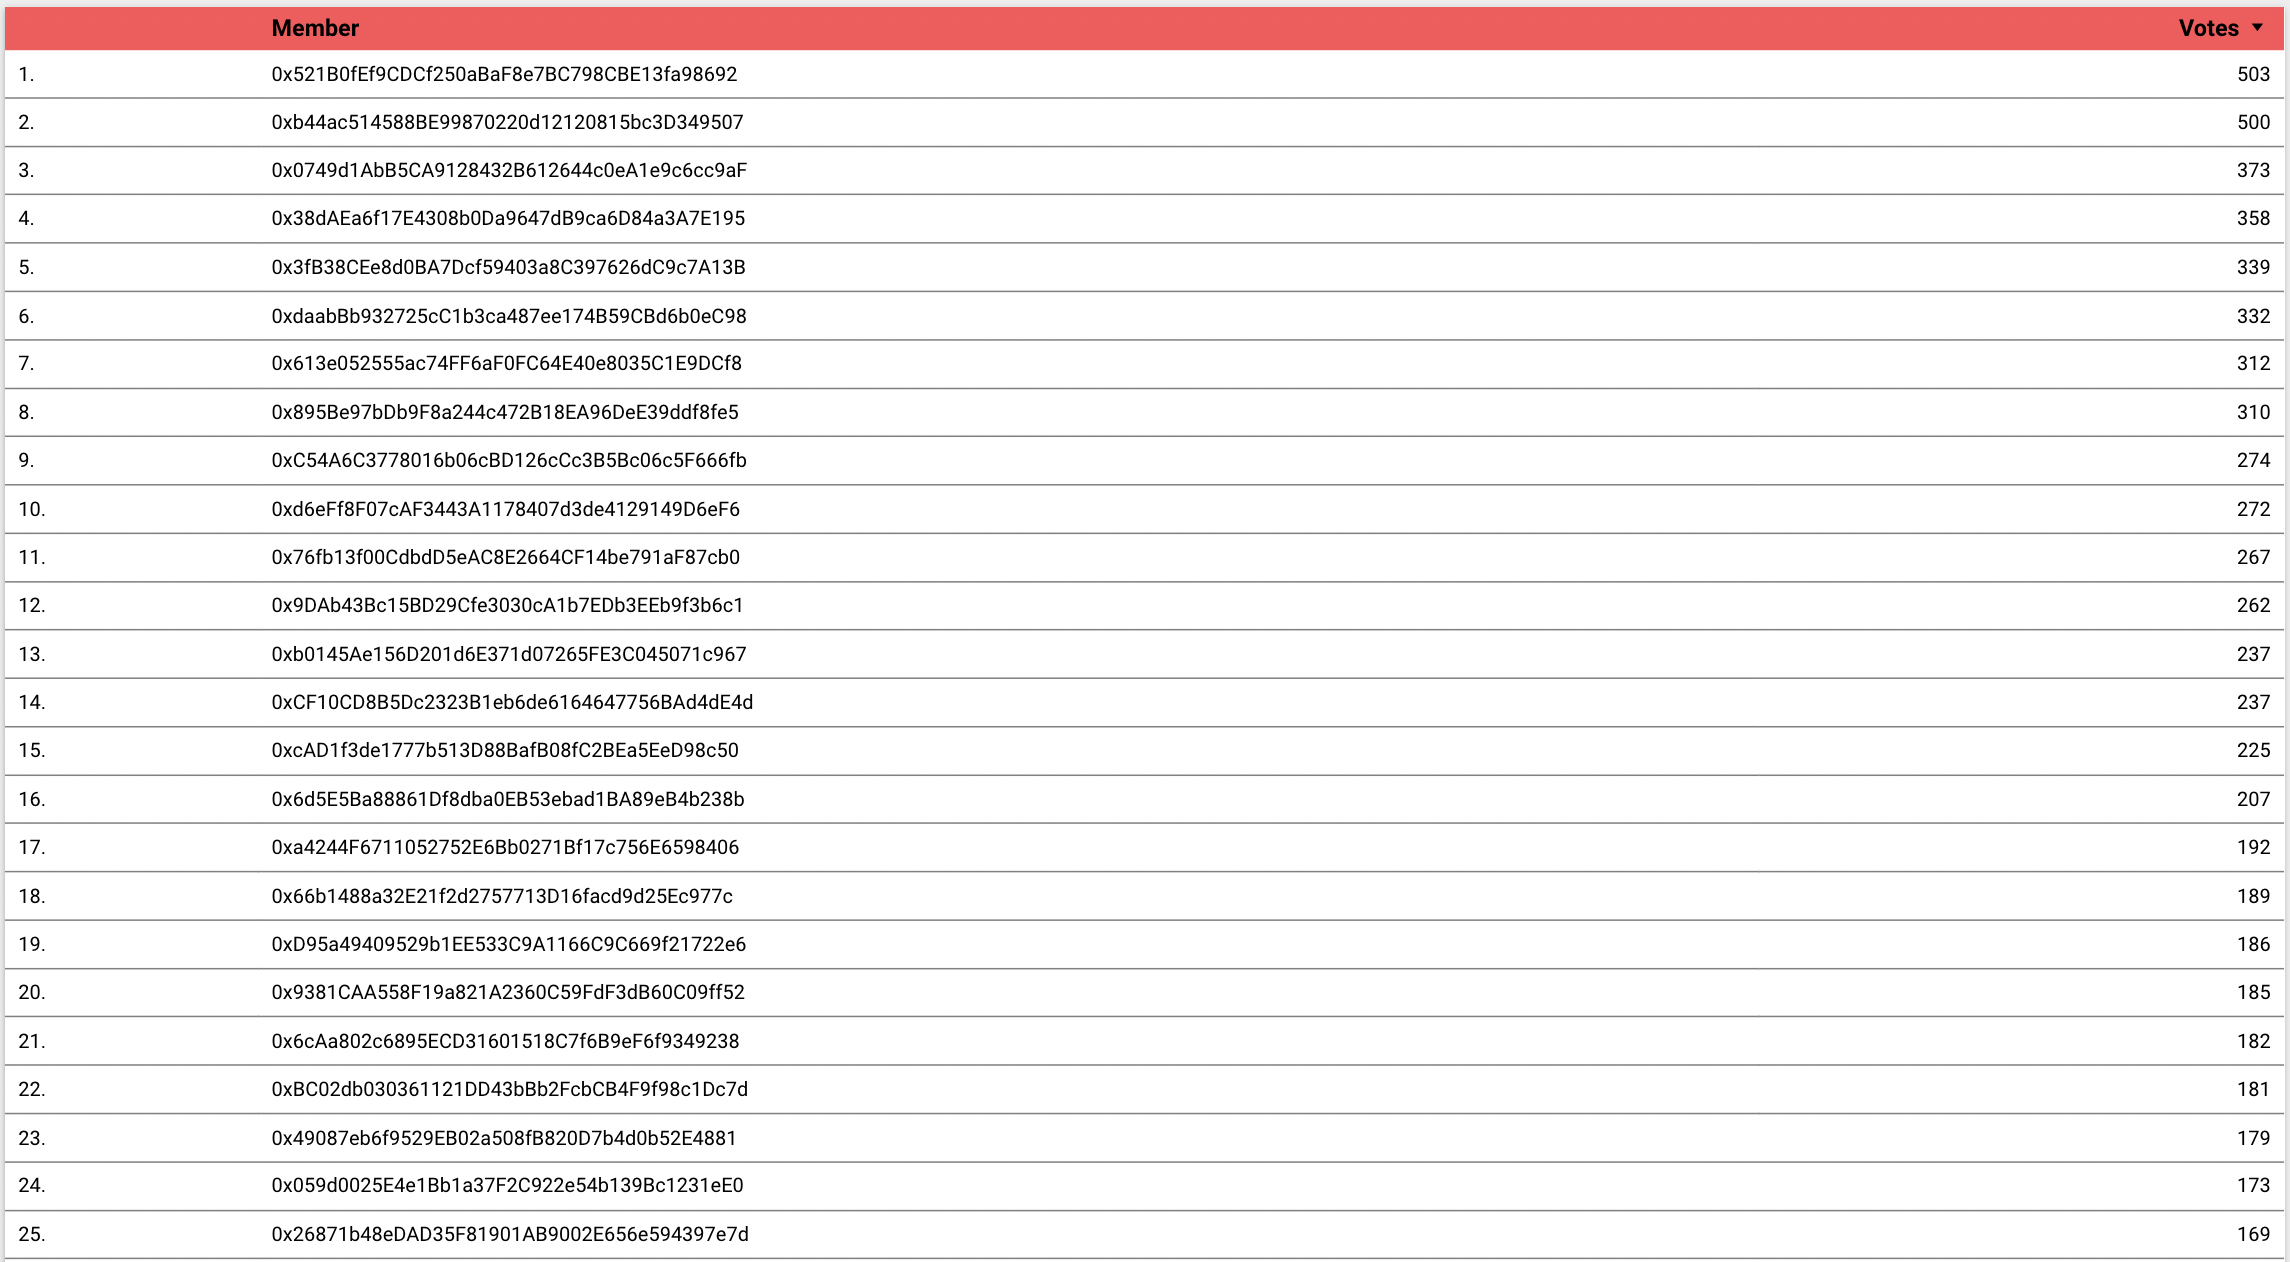
\includegraphics[width=\textwidth]{metrics/top_voters.png}
  \caption{Top 25 historical voters}
  \label{fig:top_voters}
\end{figure}

Figure \ref{fig:top_delegates} shows the top 25 to date of the addresses that received the most delegations of voting power.
\begin{figure}[H]
  \centering
  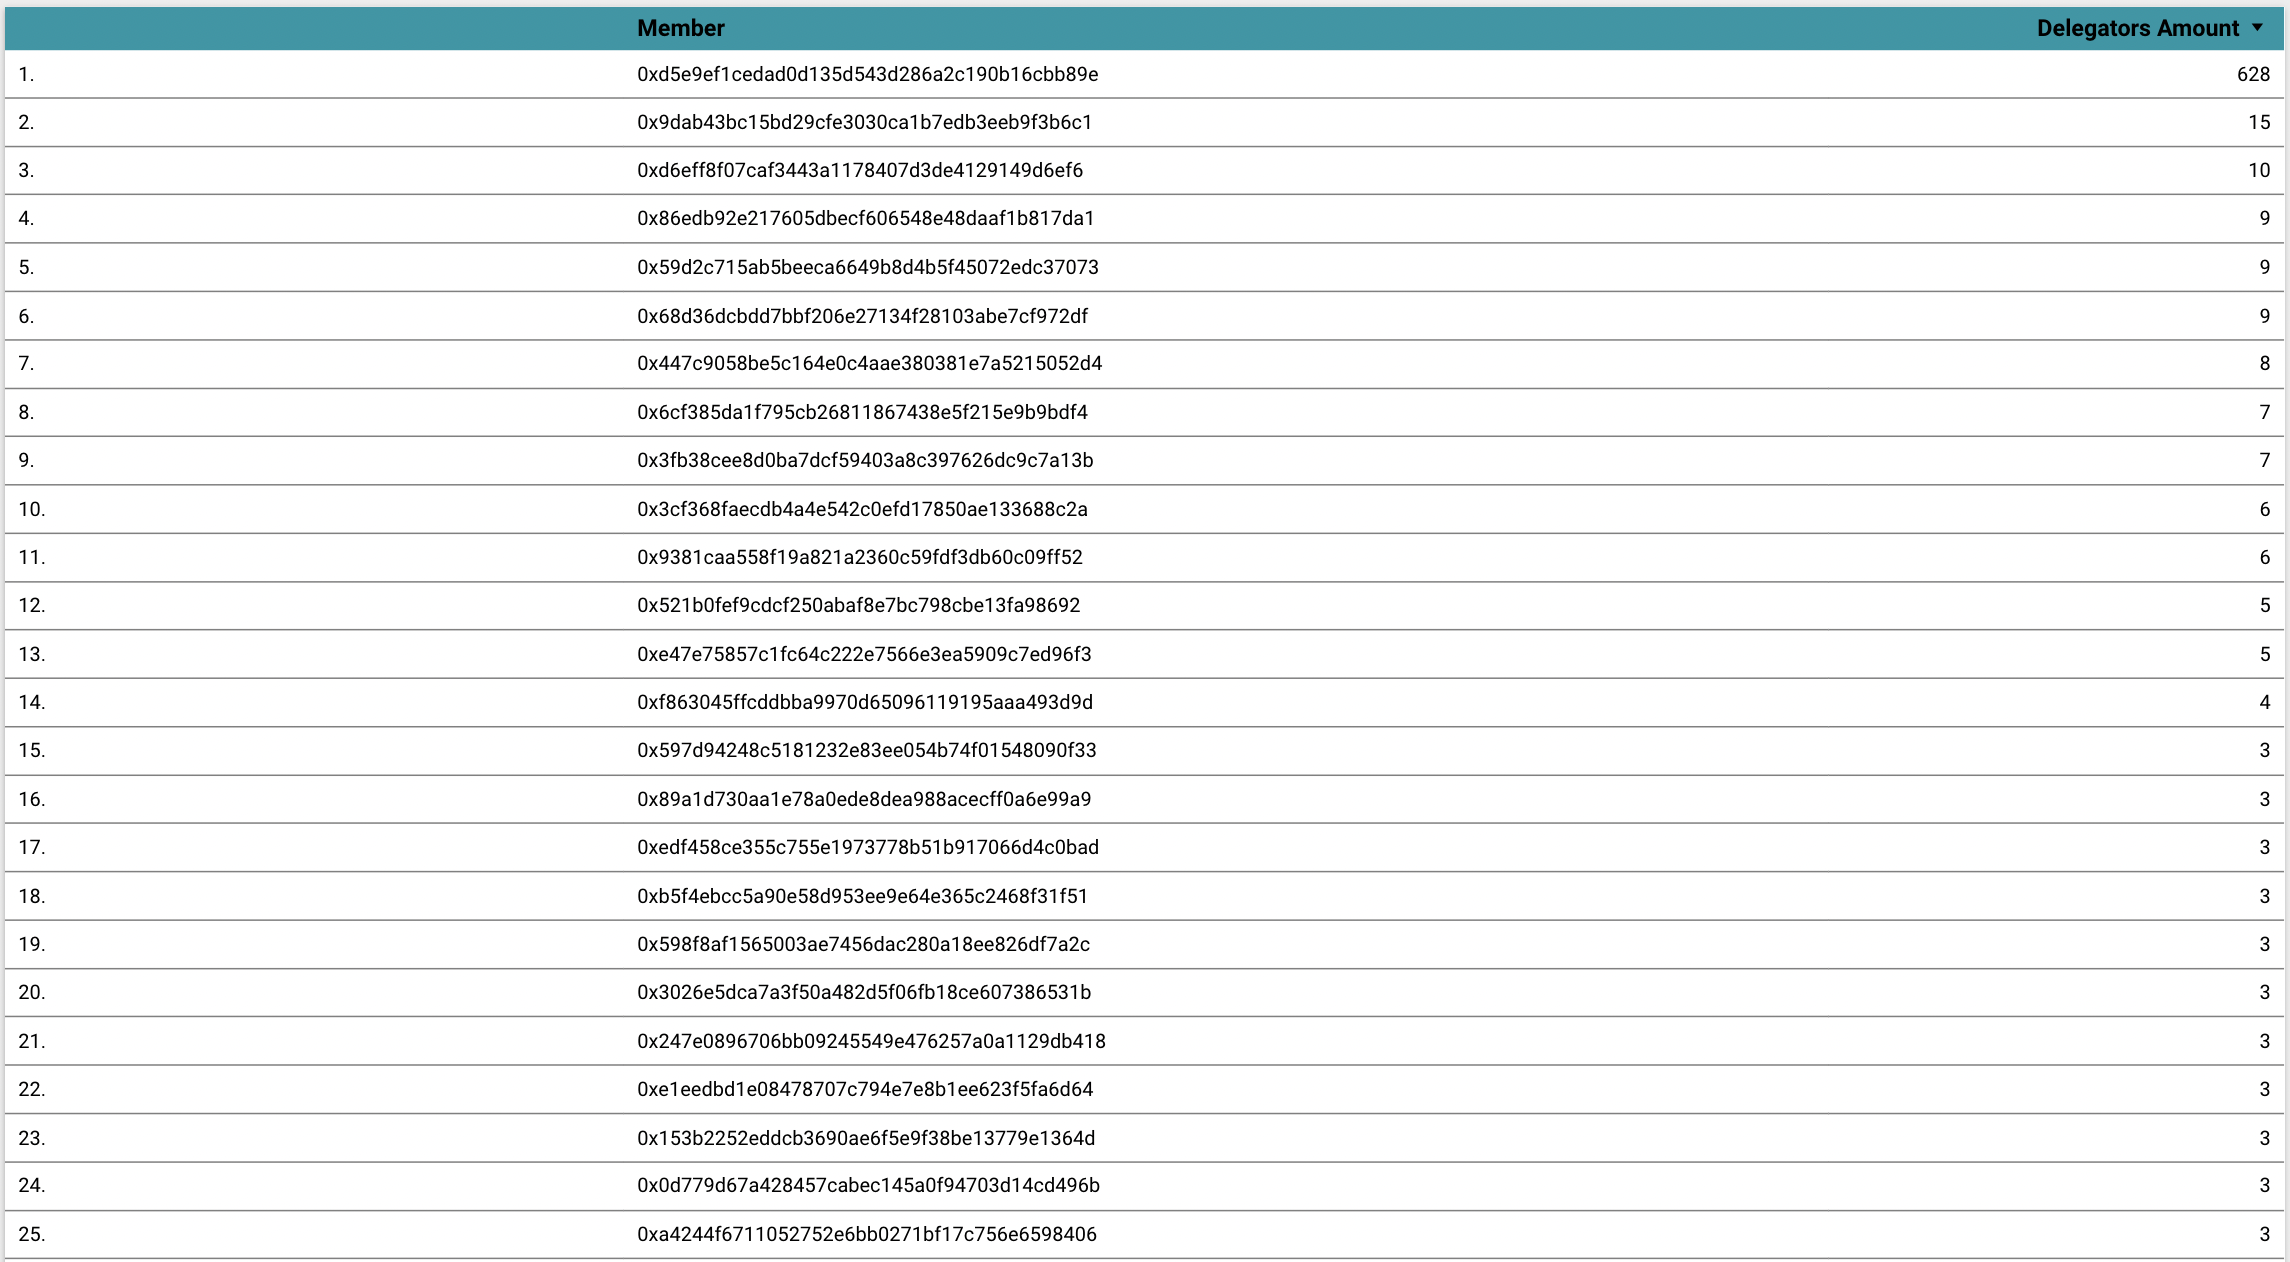
\includegraphics[width=\textwidth]{metrics/top_delegates.png}
  \caption{Top 25 delegation receivers (to date)}
  \label{fig:top_delegates}
\end{figure}

Figure \ref{fig:top_authors} shows the historical top 25 of the addresses that created the most proposals in the DAO
\begin{figure}[H]
  \centering
  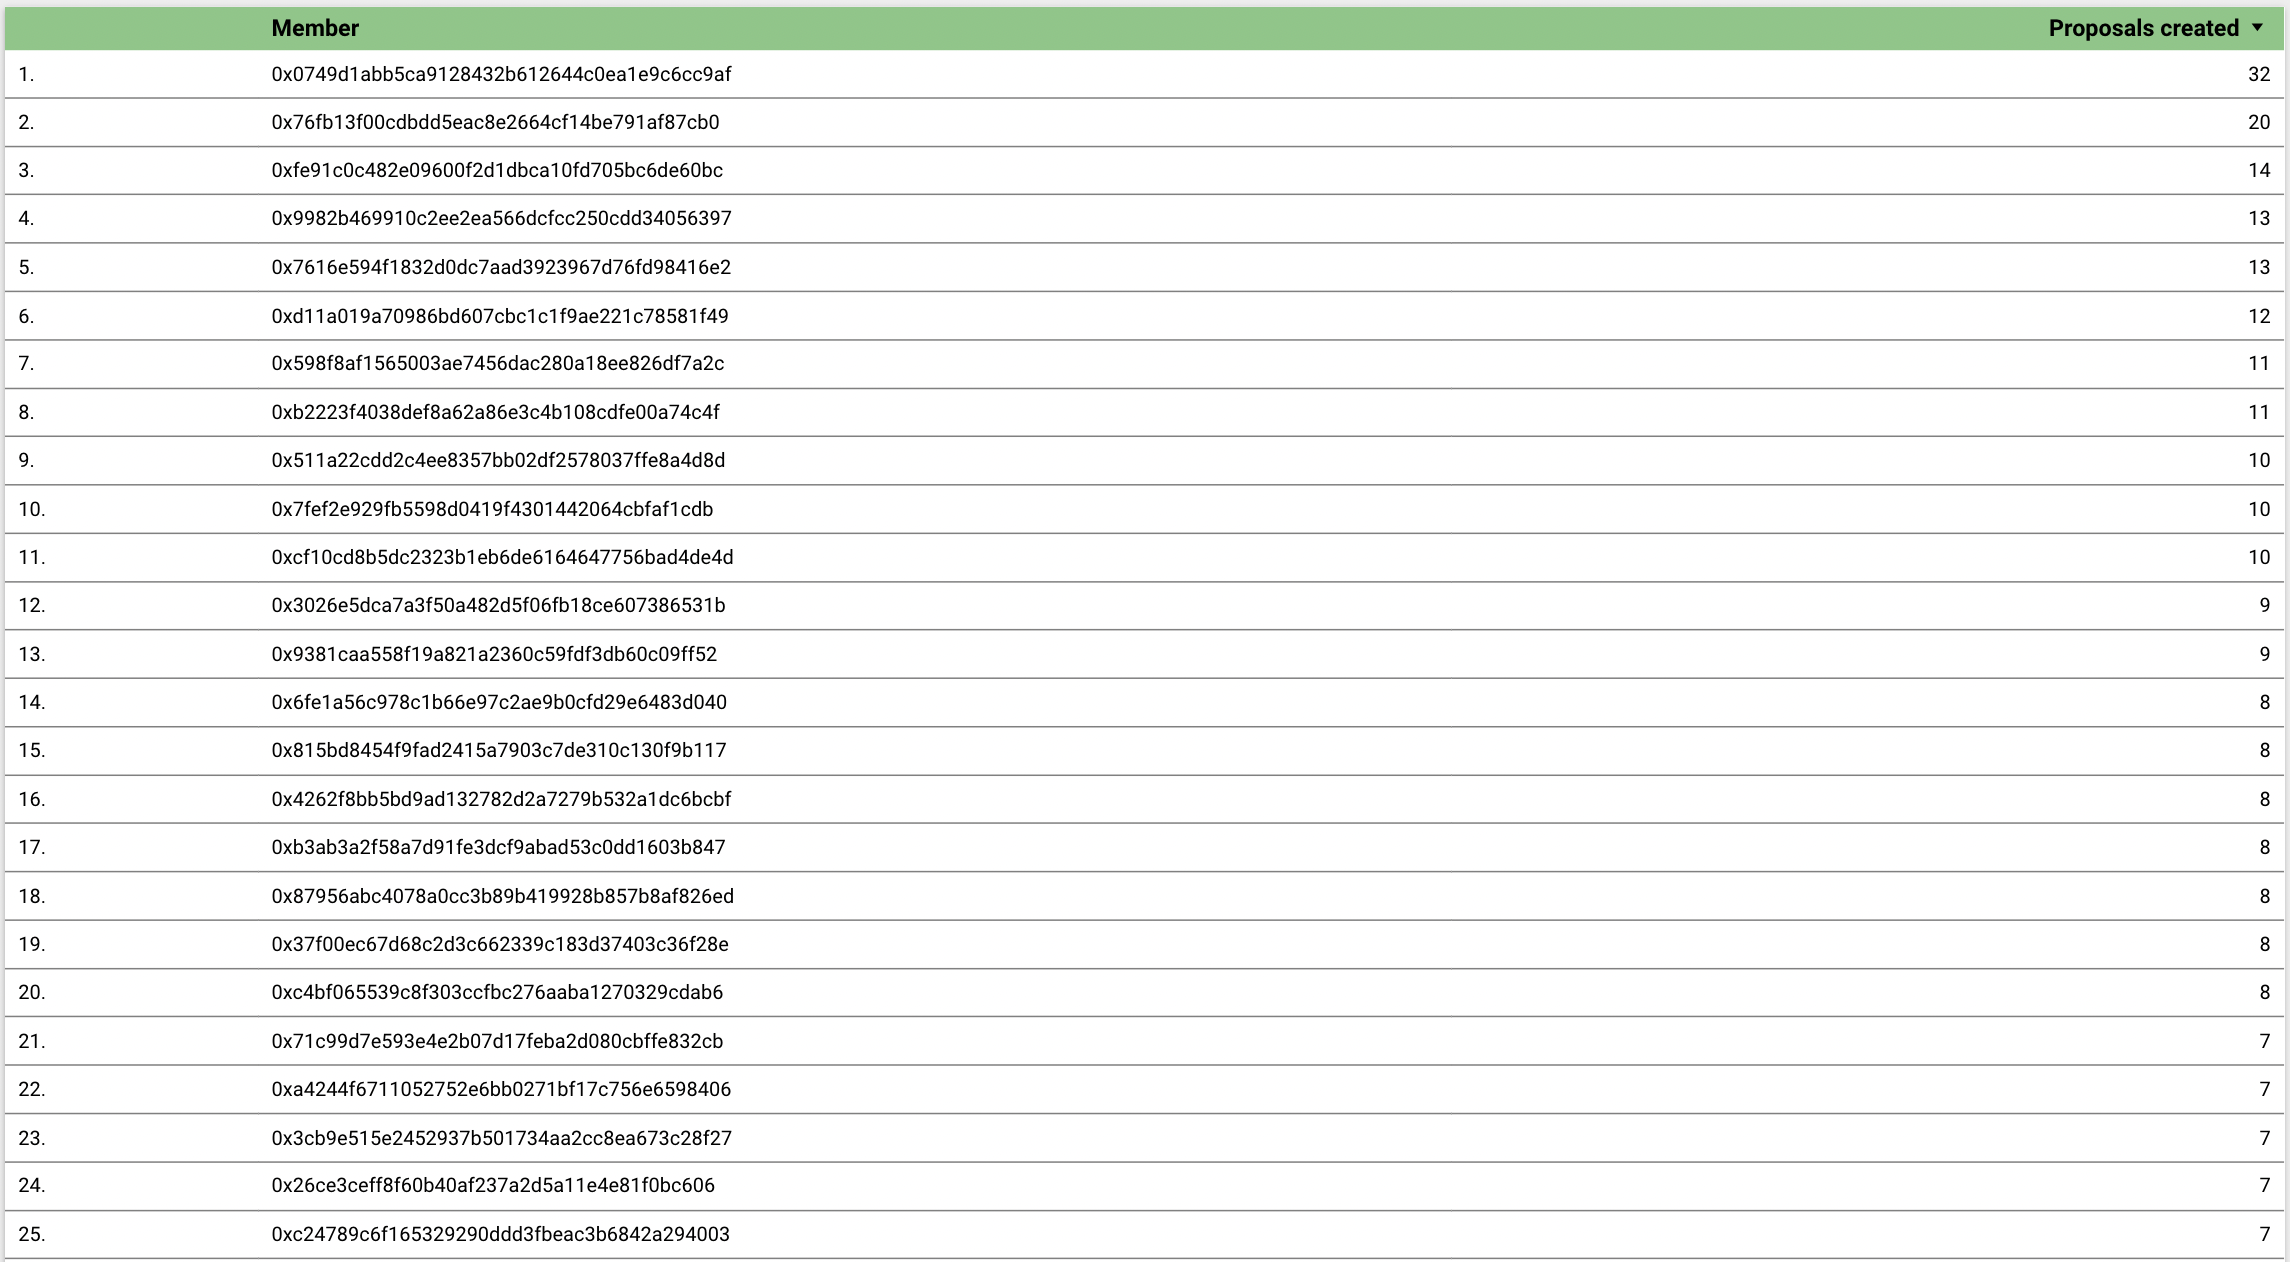
\includegraphics[width=\textwidth]{metrics/top_authors.png}
  \caption{Top 25 proposal authors (to date)}
  \label{fig:top_authors}
\end{figure}

\chapter{Conclussion\label{conclussion}}
First of all, it can be noted that extracting data from the blockchain for analysis is still not a simple task. It requires technical knowledge and programming skills to be done, so it could be said about the first research question section (see section \ref{research}) about how simple it is for an average user to access such information is that not so much.

The tools currently available to extract data are still not user-friendly enough, so an inexperienced person cannot easily access the information even if it is public. \\

Regarding the conclusions that can be drawn from the data obtained, in the first place it can be said that the DAO is still at an early stage of life, the launch date was 05/24/2021 which as of today is just over a year and a half. However, it can be seen that it is growing and that the number of members and interactions is increasing, which is a good sign. For example, Figure \ref{fig:median_votes} shows how the median number of votes per proposal is increasing month by month.

Although Figure \ref{fig:vote_weight} shows that the average voting weight in the outcome of the proposals has a decreasing trend, which gives signs of a distribution of voting power (more than 30\% is delegated as shown in Table \ref{table:VP}), Figure \ref{fig:vp_distribution_members} shows that 12 addresses concentrate more than 50\% of the voting power. While this is due to the young age of the DAO and does not necessarily represent a problem at the moment, it should not be overlooked and mechanisms should be implemented to prevent, for example, 51\% attacks\footnote{\url{https://www.coindesk.com/learn/what-is-a-51-attack/}}. 

A possible solution to this problem could be to adopt the Quadratic voting model with Sybil attack resistance used by the Gitcoin platform\footnote{\url{https://docs.passport.gitcoin.co/}}, which reduces the voting impact of addresses with a large amount of VP and, at the same time, increases the cost of splitting such VP into different addresses. \\

As for grants, the community's interest in continuing to add value to the platform is clear.  To date, 100 projects have been funded with a grand total of over US\$7 million (see Table \ref{table:grants}) - with US\$240,000 being the maximum amount allowed per grant. Figure \ref{fig:category_distribution} also shows that the distribution of categories is even.

In terms of the DAO balance sheet, the dependence on MANA (the Decentraland token) is clearly seen. As of the date of this writing, 99\% of the DAO's treasury liquidity was denominated in that token (see Figure \ref{fig:token_distribution}). Analyzing also the inflows and outflows of the DAO's wallets (Figures \ref{fig:income} and \ref{fig:expenses}), it is clear that expenses exceed income and that the only way this works is by converting the MANA from the DAO's vesting contract into stablecoins to meet expenses, which directly impacts the price of MANA. It would be interesting to find mechanisms that would allow the DAO to receive more revenue to decrease the dependence on its own token and, therefore, to avoid affecting its price when selling it. \\

Finally, a mention about the members participating in the DAO. While all the addresses that voted on at least one proposal are more than 3000, Figure \ref{fig:active_members} indicates the number of unique votes from the different addresses and shows that, on average, there are approximately 500 participants per month. This is another clear sign of the DAO's early age. As for the distribution of voting power, of the total number of DAO participants only 4.5\% delegated their voting power (see Figure \ref{fig:delegation_ratio}).

\chapter{Summary\label{summary}}
This final chapter presents a section-by-section summary of the present work.

\section{Basics}
\subsubsection{Blockchain}
The blockchain provides an immutable distributed database based on a growing sequence of blocks. These blocks, being public, form an open system that enhances trust based on the transparency and robustness of the blockchain construction technique. This database can be shared by a large number of users on a peer-to-peer basis and allows information to be stored in an immutable and orderly manner. The information added to the blockchain is public, can be accessed at any time by any user of the network and a block can only be added to the blockchain if there is an agreement between the majority of the parties.

After a certain period of time, it can be assumed that the information added to a block can no longer be modified. By design, this system intrinsically provides tolerance to node failures and robustness against manipulation and transparency, since it is public.

The removal of central authority from database structure is one of the most important and powerful aspects of blockchains. The permanence of the record is based on the permanence of the network. In the context of blockchains, this means that a large portion of a blockchain community would all have to agree to change the information and they are incentivized not to change the data.

\subsubsection{Digital Assets}
A digital asset is generally anything that is created and stored digitally, is identifiable and discoverable, and has or provides value. Digital assets have become more popular and valuable as technological advances become integrated into our personal and professional lives. Data, images, video, written content, and more have long been considered digital assets with ownership rights. Most digital items, like a company's brand, can be assigned a value, monetary or intangible.

Some digital items might only be valuable to the creator or one person, such as a family picture on your phone taken at a gathering. In the past, digital assets such as data or scanned documents were owned and used by organizations to realize value. However, when blockchain and cryptocurrency were introduced in 2009, digital assets were again redefined. Anything in digital form became something that could be used to create value via tokenization on a blockchain.

Crypto is essentially a digital currency that use blockchain technology and cryptography to facilitate secure and anonymous transactions.

\subsubsection{Smart Contracts}
A smart contract is a computerized transaction protocol that executes the terms of a contract. The general objectives of smart contract design are to satisfy common contractual conditions, minimize exceptions both malicious and accidental, and minimize the need for trusted intermediaries.

Smart contracts live on the Ethereum blockchain. They only execute when triggered by a transaction from a user. Once a smart contract is published to Ethereum, it will be online and operational for as long as Ethereum exists.

\subsubsection{Ethereum}
Ethereum is a technology for building apps and organizations, holding assets, transacting and communicating without being controlled by a central authority. There is no need to hand over personal details to use it - the user remains in control of their own data and what is being shared. Ethereum has its own cryptocurrency, Ether, which is used to pay for certain activities on the Ethereum network.

Also it is programmable using smart contracts, so that means that people can build apps that use the blockchain to store data or control what apps can do. This results in a general purpose blockchain that can be programmed to do anything.

It uses proof-of-stake, where validators explicitly stake capital in the form of ETH into a smart contract on Ethereum. This staked ETH then acts as collateral that can be destroyed if the validator behaves dishonestly or lazily. The validator is then responsible for checking that new blocks propagated over the network are valid and occasionally creating and propagating new blocks themselves.

\subsubsection{Decentralized Autonomous Organization (DAO)}
A DAO is a collectively-owned, blockchain-governed organization working towards a shared mission. It allows people to work with like-minded individuals around the globe without trusting a benevolent leader to manage the funds or operations.

Decisions are governed by proposals and voting to ensure everyone in the organization has a voice, and everything happens transparently on-chain.

\subsubsection{Metaverse}
The Metaverse is the post-reality universe, a perpetual and persistent multiuser environment merging physical reality with digital virtuality. It is based on the convergence of technologies that enable multisensory interactions with virtual environments, digital objects and people such as VR and AR. Hence, the Metaverse is an interconnected web of social, networked immersive environments in persistent multiuser platforms. It enables seamless embodied user communication in real-time and dynamic interactions with digital artifacts.

Decentraland is a decentralized virtual reality platform, better known as a metaverse, powered by the Ethereum blockchain. The finite, traversable, 3D virtual space within Decentraland is called LAND, a non-fungible digital asset or more commonly known as a NFT, maintained in an Ethereum smart contract. These parcels are permanently owned by members of the community and are purchased using MANA, Decentraland's cryptocurrency token.

The Decentraland DAO is the decision-making tool for digital assets holders in Decentraland's virtual world. Through votes in the DAO, the community can issue grants and make changes to the lists of banned names, POIs, and catalyst nodes.

\section{Methodology}
\subsubsection{Problem}
Decentraland is an open source and community driven project. Based on this, where many actors are involved in decision making, it is vital to have as much information as possible about the status of the project. Until now there was no tool or solution that could publicly provide information to everyone about the status of the DAO treasury and the different assets of the community, that is why it was essential to develop such a tool.

\subsubsection{Research Questions}
1. How easy is it for an average user to access public information on the blockchain? \\
2. What kind of analysis and conclusions can be drawn with the data obtained from the blockchain?

\subsubsection{Data collection sources}
\textbf{Decentraland's Catalyst Nodes:} A Catalyst is a Server that bundles different Services required by the Decentraland World. Each Catalyst node exposes a set of services that work as the backbone for the platform and also exposes a public API. \\

\textbf{Infura:} Is a blockchain development suite that provides application programming interfaces and developer tools. It provides fast and reliable access to the Ethereum network to enable developers to build software and Web3 applications that scale to meet user demand. \\

\textbf{The Graph:} Is a decentralized protocol for indexing and querying data from blockchains, starting with Ethereum. It makes it possible to query data that is difficult to query directly. These APIs can then be queried with a standard GraphQL API. \\

\textbf{Snapshot:} Is an off-chain gasless multi-governance client with easy to verify and hard to contest results. \\

\textbf{Covalent:} Is an indexing querying solution for blockchains that offers a diverse range of actionable insights, enabling developers to optimize the allocation of resources, bringing greater utility to decentralized applications using a single, unified API.

\section{Solution}

First, a public repository was created within the Decentraland DAO organization where the code of the scripts with their respective version history is stored. Since data must be collected every day and different sources must be consumed, Node.js was chosen for the backend of the project as it is easily configurable to run periodically in a GitHub Action. As for the programming language chosen, Typescript was used due to the versatility it offers and, naturally, for the typing - since it is very useful when working with data.

Finally, Google Data Studio is used to visualize the metrics, which uses as input the information from the CSVs collected with the scripts.

\subsubsection{Data collection scripts}

\begin{itemize}
  \item \textbf{Balances:} It's responsible for collecting the balances of the DAO's treasury. This is done by making a Covalent API call using the DAO's wallet addresses.
  \item \textbf{Collections:} It's responsible for collecting the data about all wearable collections that are currently available in Decentraland. This is done by making a GraphQL query to the corresponding subgraph of The Graph.
  \item \textbf{Curations:} It's responsible for collecting data from all wearable curations made by the curation team. This is done by making a GraphQL query to the corresponding subgraph of The Graph.
  \item \textbf{Proposals:} It's responsible for collecting data from all proposals made by the community in the DAO governance platform. This is done by combining a GraphQL query to the corresponding snapshot subgraph and an API call to the DAO platform.
  \item \textbf{Grants:} It's responsible for collecting data from all grants made by the DAO. This is done by combining multiple sources such as: the JSON file resulting from the proposals script, the Infura API to obtain information about vesting contracts, the Covalent API to obtain information about one-time-payment grant transactions, and the DAO platform to obtain information about updates made by grant beneficiaries.
  \item \textbf{Members:} It's responsible for collecting data from all members of the DAO who have voted on a proposal at least once. This is done by making a GraphQL query to the corresponding snapshot subgraph.
  \item \textbf{Transactions:} This script is the most complex of all because of the logic involved in identifying each transaction with a human-readable tag. As for the transaction data, it is collected through calls to the Covalent API.

  The strategy used to group transactions with tags basically consists of identifying the receiver or sender address depending on whether it is an OUT or IN transaction of the DAO wallets.
  
  Firstly, they were ranked by the number of times they appeared in different transactions , thus making it possible to recognize a frequency pattern. In this way, most of the transactions were identified, but many more remained. The next step was to use the output files from the grants and curations scripts to identify grant fundings and payments to curators. Finally, by reviewing transactions with large amounts of money and without a tag so far, it was possible to identify the addresses of \ac{DEXs} smart contracts for swapping tokens.
  
  About 99.95\% of the transactions could be classified into categories.
  \item \textbf{Votes:} It's responsible for collecting data from all votes made by members of the DAO. This is done by making a GraphQL query to the corresponding snapshot subgraph.
  \item \textbf{Wearables:} It's responsible for collecting data from all circulating wearables in Decentraland. This is done by making a GraphQL query to the corresponding subgraph of The Graph.
  \item \textbf{KPIs:} This script uses all the output files from the previous scripts and generates a JSON file with general DAO KPIs. This is useful to give an overview of the status of the DAO.
\end{itemize}

\subsubsection{Data visualization}
Data visualization is the representation of data through use of common graphics, such as charts, plots, infographics, and even animations. It can be utilized for a variety of purposes, and it's important to note that is not only reserved for use by data teams. Some of the types of data visualization are:

\begin{multicols}{2}
  \begin{itemize}
    \item Tables
    \item Pie charts and stacked bar charts
    \item Line charts and area charts
    \item Histograms
    \item Scatter plots
    \item Heat maps
    \item Tree maps
  \end{itemize}
\end{multicols}

\section{Conclusion}
First of all, it can be noted that extracting data from the blockchain for analysis is still not a simple task. The tools currently available to extract data are still not user-friendly enough, so an inexperienced person cannot easily access the information even if it is public.

Regarding the conclusions that can be drawn from the data obtained, in the first place it can be said that the DAO is still at an early stage of life, the launch date was 05/24/2021 which as of today is just over a year and a half. However, it can be seen that it is growing and that the number of members and interactions is increasing, which is a good sign.

As for grants, the community's interest in continuing to add value to the platform is clear. To date, 100 projects have been funded with a grand total of over US\$7 million - with US\$240,000 being the maximum amount allowed per grant.

In terms of the DAO balance sheet, the dependence on MANA is clearly seen. Analyzing the inflows and outflows of the DAO's wallets, it is clear that expenses exceed income and that the only way this works is by converting the MANA from the DAO's vesting contract into stablecoins to meet expenses, which directly impacts the price of MANA.

As for the distribution of voting power, of the total number of DAO participants only 4.5\% delegated their voting power.

\section{What's next?}
The next steps of this project are to continue collecting data and analyzing it to obtain more insights, given that there is still just over a year's worth of data. In addition, it is planned to add new charts that will continue to add details on the status of the DAO. 

It is also intended to be able to collect this information in real time, since at the moment these scripts run once a day.

\toComplete

\chapter{Glossary}
\printnoidxglossaries
\clearpage

\printbibliography
\clearpage

\listoffigures
\clearpage

\listoftables
\clearpage

\listofcode
\clearpage

\phantomsection
\addcontentsline{toc}{chapter}{\listacroname}
\chapter*{\listacroname}
\begin{acronym}
    \acro{Crypto}{Cryptocurrency}
    \acro{Dapp}{Decentralized App}
    \acro{DAO}{Decentralized Autonomous Organization}
    \acro{NFT}{Non-Fungible Token}
    \acro{PoW}{Proof-of-Work}
    \acro{PoS}{Proof-of-Stake}
    \acro{VR}{Virtual Reality}
    \acro{AR}{Augmented Reality}
    \acro{L2}{Layer 2}
    \acro{DEXs}{Decentralized Exchanges}
\end{acronym}

\clearpage
\appendix
\end{document}
